\chapter{Analyse} % Main chapter title

\label{K6} % Change X to a consecutive number; for referencing this chapter elsewhere, use \ref{ChapterX}
\begin{sloppypar}
Dieses Kapitel ist der Analyse der einzelnen Studienelemente gewidmet. Zu Anfang werden die Ergebnisse der Online-Umfrage\is{Umfrage!online} zum Nutzungsverhalten von Skype\is{Skype} dargestellt und situiert (Abschnitt \ref{K6:sec:UmfrageAllg}). Danach werden die Angaben im Ein- und Ausgangsfragebogen\is{Fragebogen!Eingangs-}\is{Fragebogen!Ausgangs-} der Proband{\textperiodcentered}innen im katalanisch-deutschen Versuchsaufbau betrachtet (Abschnitt \ref{K6:sec:Probandinnen-CatDe}, S.\,\pageref{K6:sec:Probandinnen-CatDe}), bevor sich die Analyse den Eye-Tracking-Daten dieses Versuchsteils zuwendet (Abschnitt \ref{K6:sec:DatenCatDe}, S.\,\pageref{K6:sec:DatenCatDe}). Zuletzt werden in gleicher Abfolge die Angaben und Daten aus dem Setting Deutsch-Deutsch betrachtet (Abschnitte \ref{K6:sec:Probandinnen-DeDe}, S.\,\pageref{K6:sec:Probandinnen-DeDe} und \ref{K6:sec:DatenDeDe}, S.\,\pageref{K6:sec:DatenDeDe}).
\end{sloppypar}
%------------------------------------------------------

\section{Online-Umfrage zur allgemeinen Nutzung von Skype}

\label{K6:sec:UmfrageAllg}

%------------------------------------------------------

Die Umfrage\is{Umfrage} zum Nutzungsverhalten von Skype\is{Skype} wurde im Zeitraum von Mai bis Juli 2018 durchgeführt. In diesem Zeitraum nahmen 329 Personen teil, von denen 290 den Fragebogen komplett ausfüllten. Verglichen mit den Angaben des Statistischen Bundesamtes\is{Statistisches Bundesamt}, nach denen im Zeitraum des Wintersemesters des betreffenden Zeitraums (2017/18) 2.847.000 Student{\textperiodcentered}innen an deutschen Hochschulen eingeschrieben waren, stellt diese Erhebung keine repräsentative Stichprobe dar\footnote{Vgl. \url{https://www.destatis.de/DE/Presse/Pressemitteilungen/2017/11/PD17_427_213.html}, letzter Abruf am \datum{}.}. Die folgenden Angaben stützen sich außerdem -- sofern nicht anders angegeben~-- ausschließlich auf diese 290 vollständigen Datensätze.

%------------------------------------------------------

\subsection{Ergebnisse der Umfrage}

\label{K6:subsec:Ergebnisse-Umfrage}

%------------------------------------------------------
%------------------------------------------------------

%\subsubsection{Grundlegendes} % SubSubSection auskommentiert, weil einzige Überschrift in dieser Hierarchie.

\label{K6:subsub:Grundlegendes-Umfrageergebnisse}

% https://astt.fb06.uni-mainz.de/files/2019/12/Band25_VerbleibsstudieDesFTSKGermersheim2.pdf
% https://www.forschung-und-lehre.de/lehre/studierende-im-schnitt-23-4-jahre-alt-3163/

%------------------------------------------------------

Von den Teilnehmer{\textperiodcentered}innen gaben 222 an, weiblich und 64 männlich zu sein. 4 enthielten sich der Angabe. Das entspricht einer Geschlechterverteilung von 77\,\% zu 22\,\% zu 1\,\%.\footnote{Die Abfrage des Geschlechts erfolgte zu einem Zeitpunkt, als es in Deutschland noch nicht absehbar war, dass ein sog. \emph{drittes Geschlecht} mit der Bezeichnung \emph{divers} eingeführt würde. Daher konnten die teilnehmenden Personen nur zwischen \emph{männlich}, \emph{weiblich} und \emph{sonstiges} wählen, oder sich der Antwort enthalten (s.\,a.\ Anhang\,\ref{App1:SectionDemographie}, Frage 36).}

Teilt man die Datensätze nach Alter in Dekaden ein, so erhält man eine Verteilung wie in der Alterspyramide in \figref{K6:fig:alterspyramide} dargestellt. Der Altersdurchschnitt liegt bei 25,72, der Median bei 24,00 Jahren. Damit liegt der Altersschnitt über dem der im Wintersemester 2019/20 regulär in Deutschland eingeschriebenen Studierenden. Dieser beträgt 23,4 Jahre\footnote{S. \url{https://www.forschung-und-lehre.de/lehre/studierende-im-schnitt-23-4-jahre-alt-3163/}, letzter Abruf am \datum{}.} Das erste und dritte Quartil liegt bei jeweils 22,00 und 27,00 Jahren. Eine Person gab ein Alter von 2 Jahren an. Hier lässt sich eine Falscheingabe oder ein Anonymisierungsversuch vermuten. Am oberen Ende der Alterspyramide liegt eine Person mit 71 Jahren. Ein Erklärungsansatz könnte hier zum emeritierten Lehrpersonal oder zu den Angeboten der sog. Senioren-Universität führen. Auch wenn die überwiegende Mehrheit der Teilnehmer{\textperiodcentered}innen im für Student{\textperiodcentered}innen typischen Alter liegt, zeigt die demographische Angabe ebenfalls, dass eine ausschließliche Adressierung der Online-Umfrage an Student{\textperiodcentered}innen kaum bis unmöglich ist.

%------------------------------------------------------
% Alterspyramide

\begin{figure}
    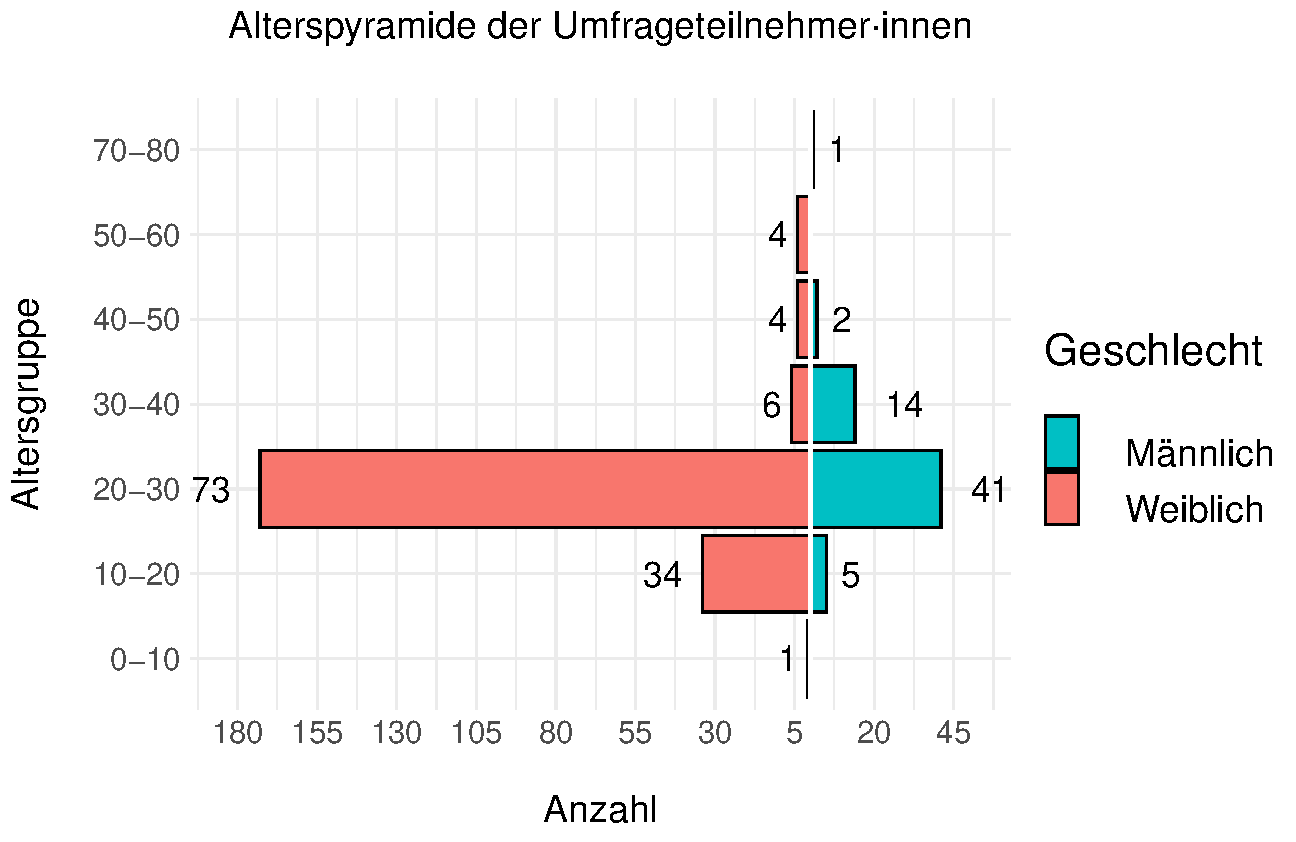
\includegraphics[width=.85\textwidth]{Figures/Umfrage/GGplot/ggplot_alterspyramide}
    \caption{Alterspyramide der Teilnehmer\label{K6:fig:alterspyramide}}
\end{figure}

%------------------------------------------------------

Dies lässt sich auch anhand der Angaben zum höchsten Abschluss erkennen. Die Abkürzungen entlang der X-Achse stehen der Reihenfolge nach für eine abgeschlossene Ausbildung (\emph{Abg.A.}), die mittlere Reife (\emph{mit.R.}), einen höheren Berufsabschluss (\emph{höh.B.}), die Hochschulzugangsberechtigung (\emph{HZB}) und einen Hochschulabschluss (\emph{HSA}). In Bezug auf die Frage gaben 270 Personen an, entweder die Hochschulzugangsberechtigung erlangt oder bereits ein Studium (i.\,S.\,v.\ Bachelor, Master, Diplom o.\,ä.) abgeschlossen zu haben. Weitere 12 der verbleibenden 20 Teilnehmer{\textperiodcentered}innen gaben an, eine Ausbildung abgeschlossen zu haben. Somit ist auch hier erkennbar, dass zwar einerseits überwiegend die Zielgruppe angesprochen, zugleich jedoch auch vereinzelt Personen teilgenommen haben, die nachweislich nicht zur intendierten Gruppe gehören (s. \figref{K6:fig:Abschluss-nw}).

%------------------------------------------------------------------------
% Abschluss und Geschlecht

\begin{figure}
		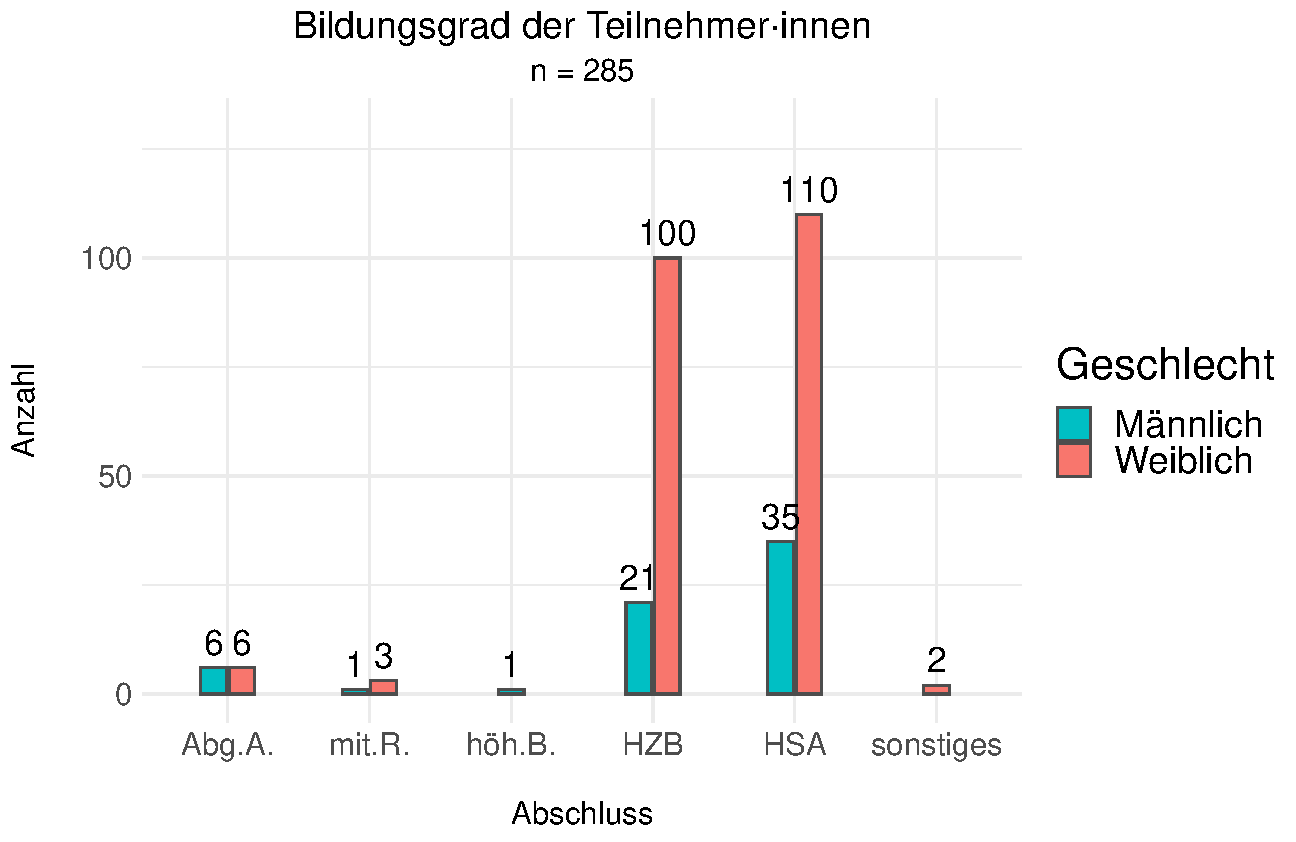
\includegraphics[width=.85\textwidth]{Figures/Umfrage/GGplot/ggplot_Geschlecht-Abschluss}
	\caption{Höchster Abschluss nach Geschlecht\label{K6:fig:Abschluss-nw}}
\end{figure}

%------------------------------------------------------------------------

Die Mehrheit der Teilnehmer{\textperiodcentered}innen (254/290) gab Deutsch als die Sprache an, mit der sie primär aufgewachsen seien. Diese Werte sind nicht deckungsgleich mit der im Alltag hauptsächlich verwendeten Sprache. Hier gaben 238 Personen an, hauptsächlich Deutsch zu verwenden, weitere zehn setzten Deutsch und Englisch gleich. Die verbleibenden Umfrageteilnehmer{\textperiodcentered}innen gaben ausschließlich Englisch oder eine gänzlich andere Sprache an. Ebenso verhielt es sich bei der im Beruf hauptsächlich verwendeten Sprache, als welche 208 Personen Deutsch angaben, sechs sowohl Deutsch und Englisch und 19 ausschließlich Englisch. Die verbleibenden Personen gaben auch hier eine andere Sprache an. Eine dritte Frage konzentrierte sich auf weitere Fremdsprachen, sofern die Umfrageteilnehmer{\textperiodcentered}innen einen offiziellen Nachweis über das Niveau besaßen. Hierbei wurden 36 verschiedene Sprachen angegeben, die in \figref{K6:fig:Fremdsprachen-Umfrage} aufgeschlüsselt sind. Bereits während der Auswertung wurden die Angaben bereinigt: Anmerkungen zur eigenen Einschätzung des Kompetenzniveaus der Proband{\textperiodcentered}innen und Angaben zum offiziellen Nachweis wurden ebenso wie Orthographiefehler entfernt.

%------------------------------------------------------------------------
% Weitere Fremdsprachen

\begin{figure}
		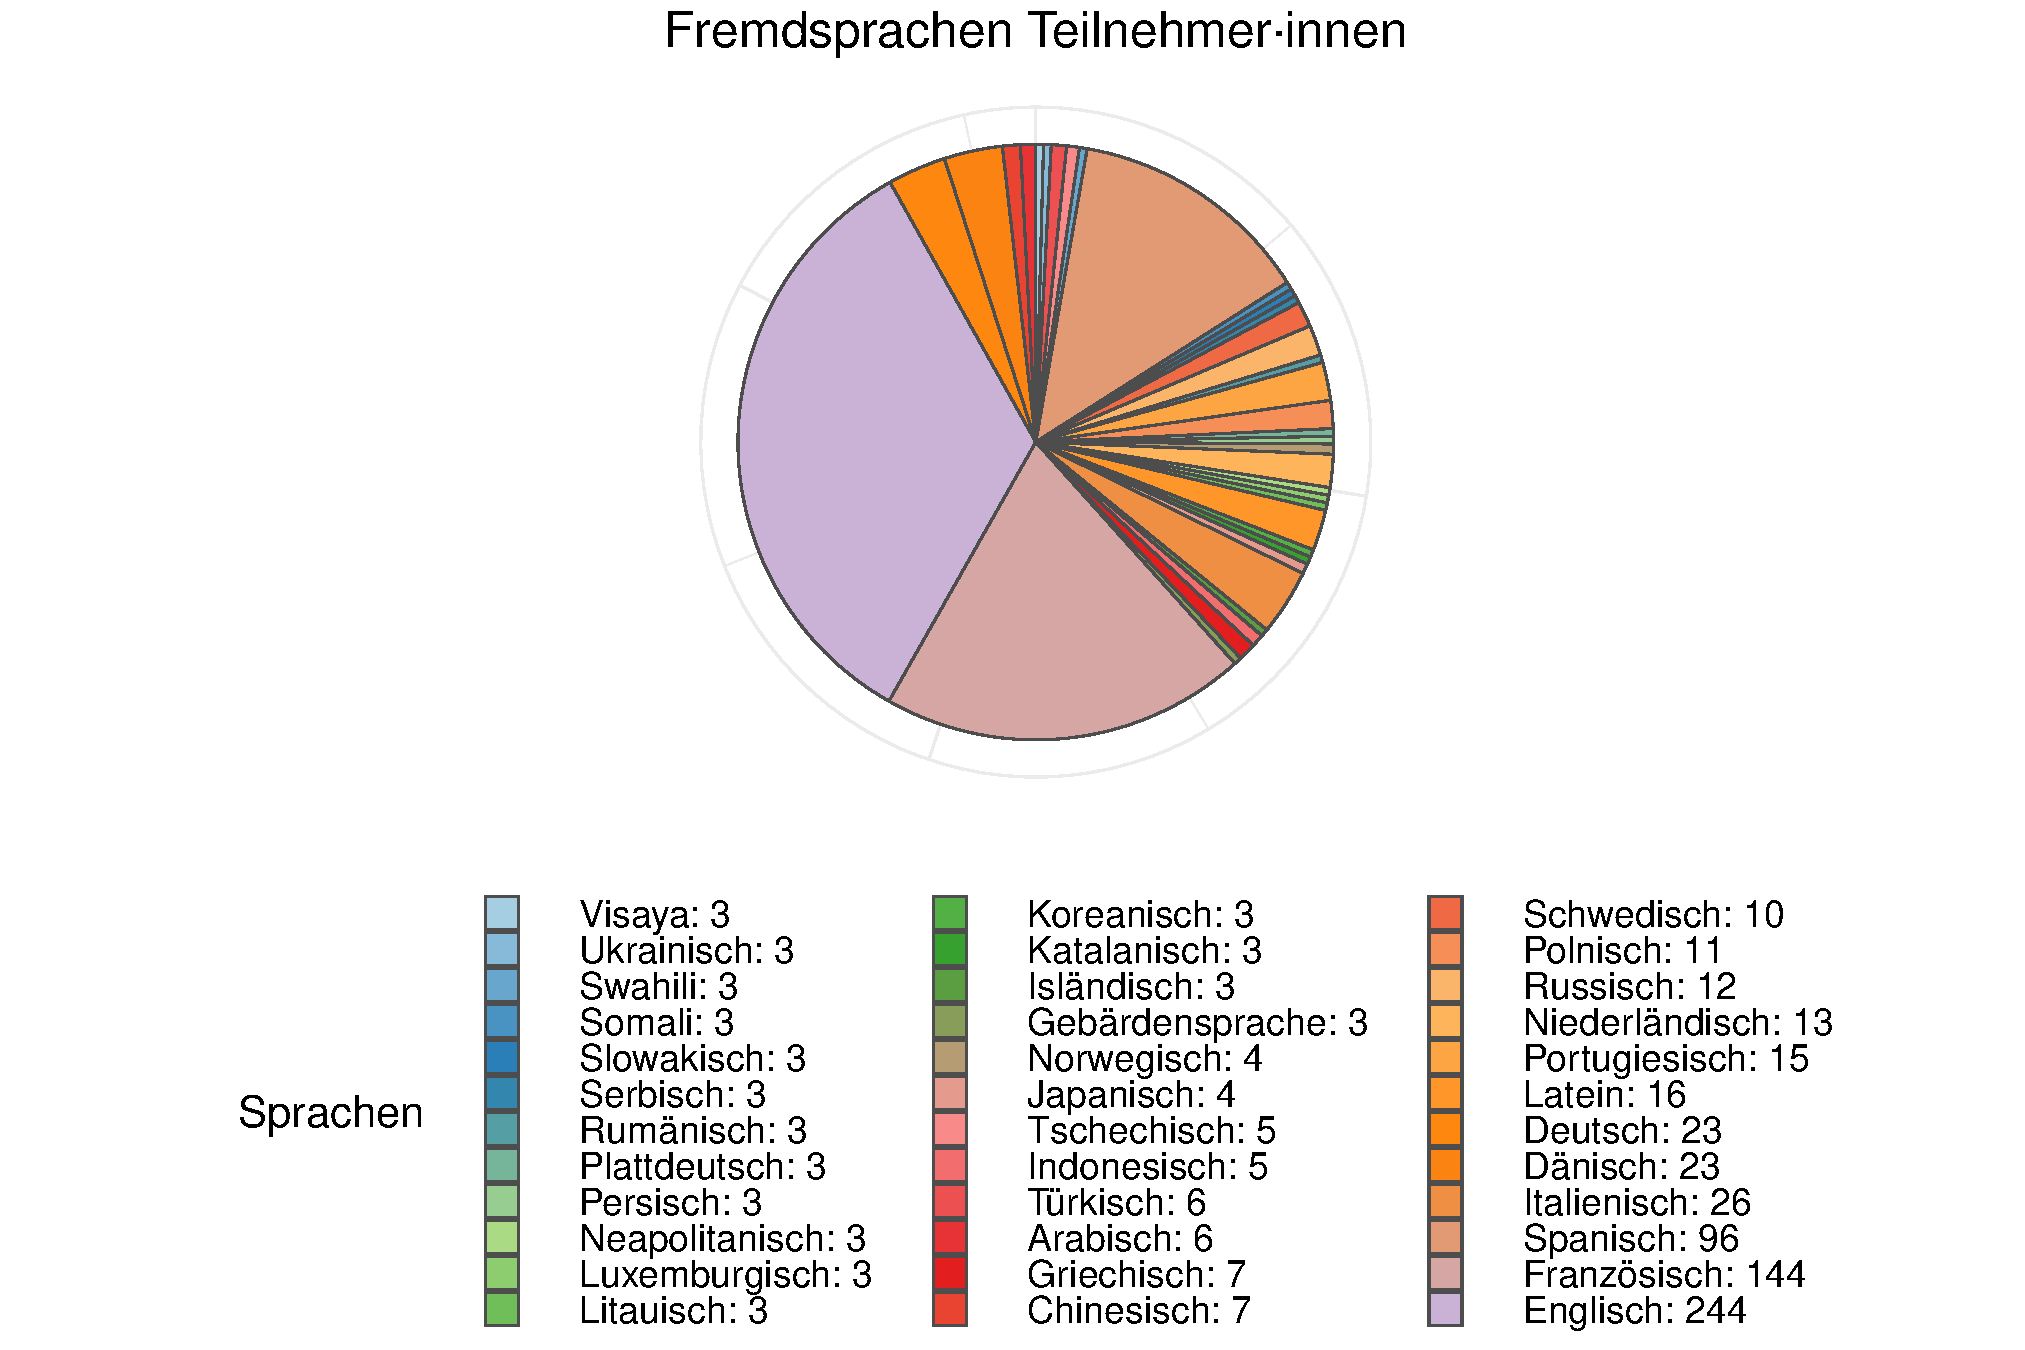
\includegraphics[width=\textwidth]{Figures/Umfrage/GGplot/ggplot_sprachen_TN-Umfrage}
	\caption{Weitere Fremdsprachen der Teilnehmer{\textperiodcentered}innen\label{K6:fig:Fremdsprachen-Umfrage}}
\end{figure}

%------------------------------------------------------------------------

167 von 290 Umfrageteilnehmer{\textperiodcentered}innen gaben weiterhin an, bereits längere Zeit (mehr als vier Wochen Minimum, kein Urlaub) im Ausland verbracht zu haben. Insgesamt wurden 120 verschiedene Länder genannt. Die in den jeweiligen Ländern verbrachte Dauer reicht von einem bis 576 Monate (entspricht 48 Jahren, \diameter\,34,5 Monate, Median = 13 Monate, SD = 77,17). Als Gründe wurden Spracherwerb (52/290), Sprachvertiefung (91/290), Kulturkontakt (84/290), ein Pflichtaufenthalt (20/290), eine Fortbildung (20/290), berufliche Motivation (39/290) sowie die (zeitweise) Verlagerung des Lebensmittelpunktes (35/290) genannt. Die Aufenthalte lagen dabei zwischen weniger als einem und 360 Monaten zurück (\diameter\,32,5 Monate, Median = 22,5 Monate, SD = 42,5).

%%%%%%%%%%%%%%%%%%%%%%%%%%%%%%%%%%%%%%%%%%%%%%%%%
% https://www.destatis.de/DE/Themen/Gesellschaft-Umwelt/Bildung-Forschung-Kultur/Hochschulen/Publikationen/Downloads-Hochschulen/studierende-ausland-5217101187004.pdf?__blob=publicationFile
% https://www2.daad.de/presse/pressemitteilungen/de/32116-immer-mehr-deutsche-studieren-im-ausland/
% https://www.studentenwerke.de/de/content/internationalisierung-zahlen
% https://de.statista.com/statistik/daten/studie/167055/umfrage/deutsche-studierende-im-ausland-nach-studienland/
% https://de.statista.com/statistik/daten/studie/1079332/umfrage/umfrage-zu-den-gruenden-fuer-einen-umzug-ins-ausland/
% https://de.statista.com/infografik/7792/die-10-beliebtesten-ziele-fuers-auslandssemester/
% https://imperia.daad.com/medien/eu.daad.de.2016/dokumente/service/medien-und-publikationen/jahresberichte/erasmusplus_jahresbericht_2019.pdf
%%%%%%%%%%%%%%%%%%%%%%%%%%%%%%%%%%%%%%%%%%%%%%%%%


%------------------------------------------------------------------------

\subsection{Generelle Nutzungsangaben}

\label{K6:sub:Gen-Nutzungsan}

%------------------------------------------------------------------------

Von 290 Teilnehmer{\textperiodcentered}innen an der Umfrage gaben 227 an, Skype\is{Skype|(} überhaupt zu nutzen (s. \figref{K6:fig:Nutzungsh-mw}). Da die Online-Umfrage so konditioniert war, dass nur die Teilnehmer{\textperiodcentered}innen an der Umfrage den Fragenblock zu den Nutzungsgewohnheiten im Umgang mit Skype eingeblendet bekamen, beziehen sich zunächst alle folgenden Angaben auf diese 227 Personen. Mit ca. 73,6\,\% nutzte deutlich mehr als die Hälfte der Umfrageteilnehmer{\textperiodcentered}innen Skype entweder seltener als monatlich (143/227) oder nahezu monatlich (43/227). 40 Personen (18,5\,\%) gaben an, Skype wöchentlich nutzen und weitere 18 (7,9\,\%) nutzen es laut eigenen Angaben täglich. Auffälligerweise wählten zwei Personen (0,9\,\%) die Antwortmöglichkeit \emph{Nie}, auch wenn sie zuvor auf die Frage, ob sie Skype nutzten, mit \emph{Ja} geantwortet haben müssen (s. \figref{K6:fig:Nutzungsh-mw}).

In Bezug auf die Frage nach der Nutzungsdauer pro Sitzung gaben 165 Teilnehmer{\textperiodcentered}innen (72,7\,\%) an, die Anwendung entweder länger als eine Stunde (85/227) oder mindestens eine Stunde (80/227) zu verwenden. Eine kürzere Sitzungsdauer in den Kategorien \emph{bis zu 30 Minuten}, \emph{bis zu 15 Minuten} und \emph{bis zu 5 Minuten} wurde jeweils von 34 (15\,\%), 16 (7\,\%) bzw. 8 (3,5\,\%) Personen angegeben. Vier Personen enthielten sich der Antwort.

%------------------------------------------------------------------------
% Nutzungshaeufigkeit

\begin{figure}
		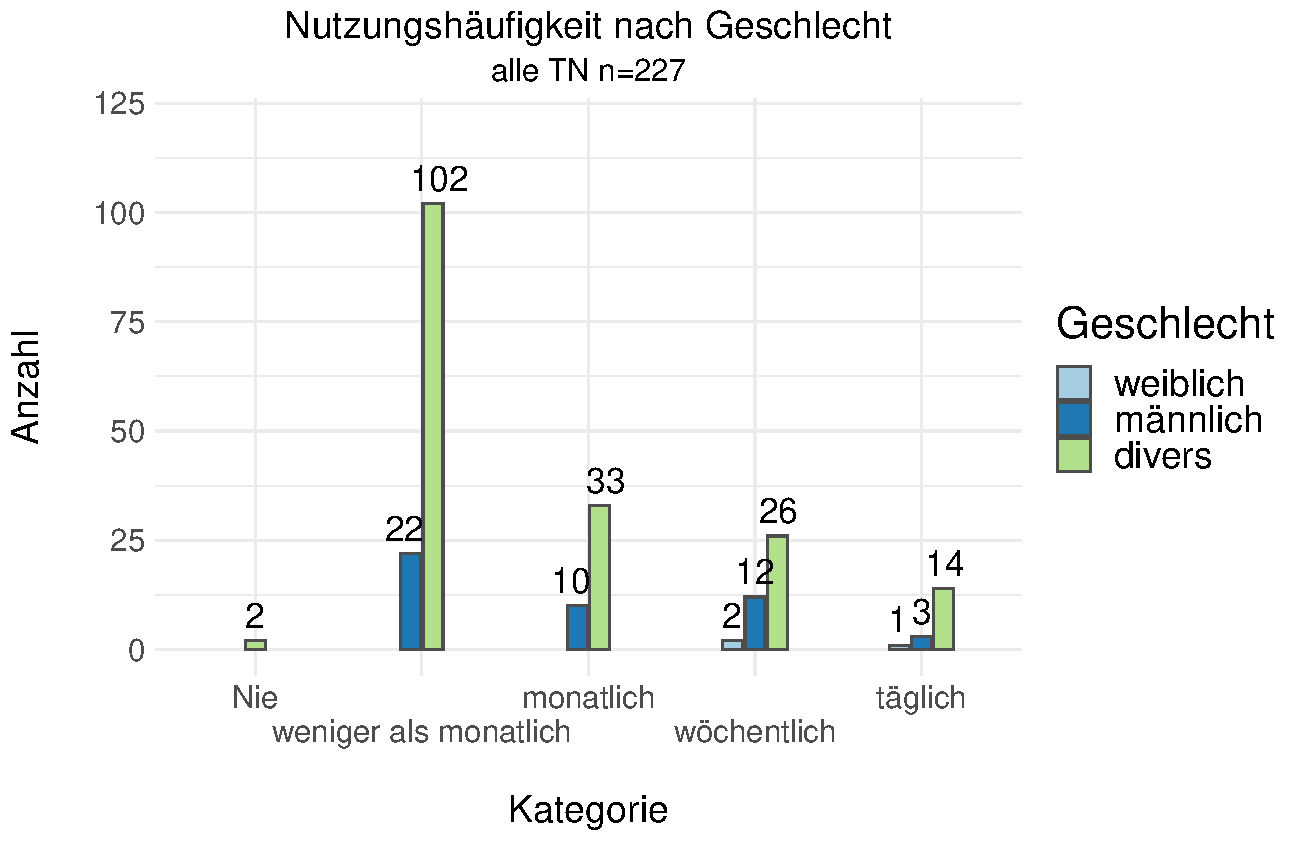
\includegraphics[width=.85\textwidth]{Figures/Umfrage/GGplot/ggplot_Geschlecht-Nutzungsh}
	\caption{Nutzungshäufigkeit nach Geschlecht\label{K6:fig:Nutzungsh-mw}}
\end{figure}

%------------------------------------------------------------------------

%------------------------------------------------------------------------
% Plattform

\begin{figure}[p]
    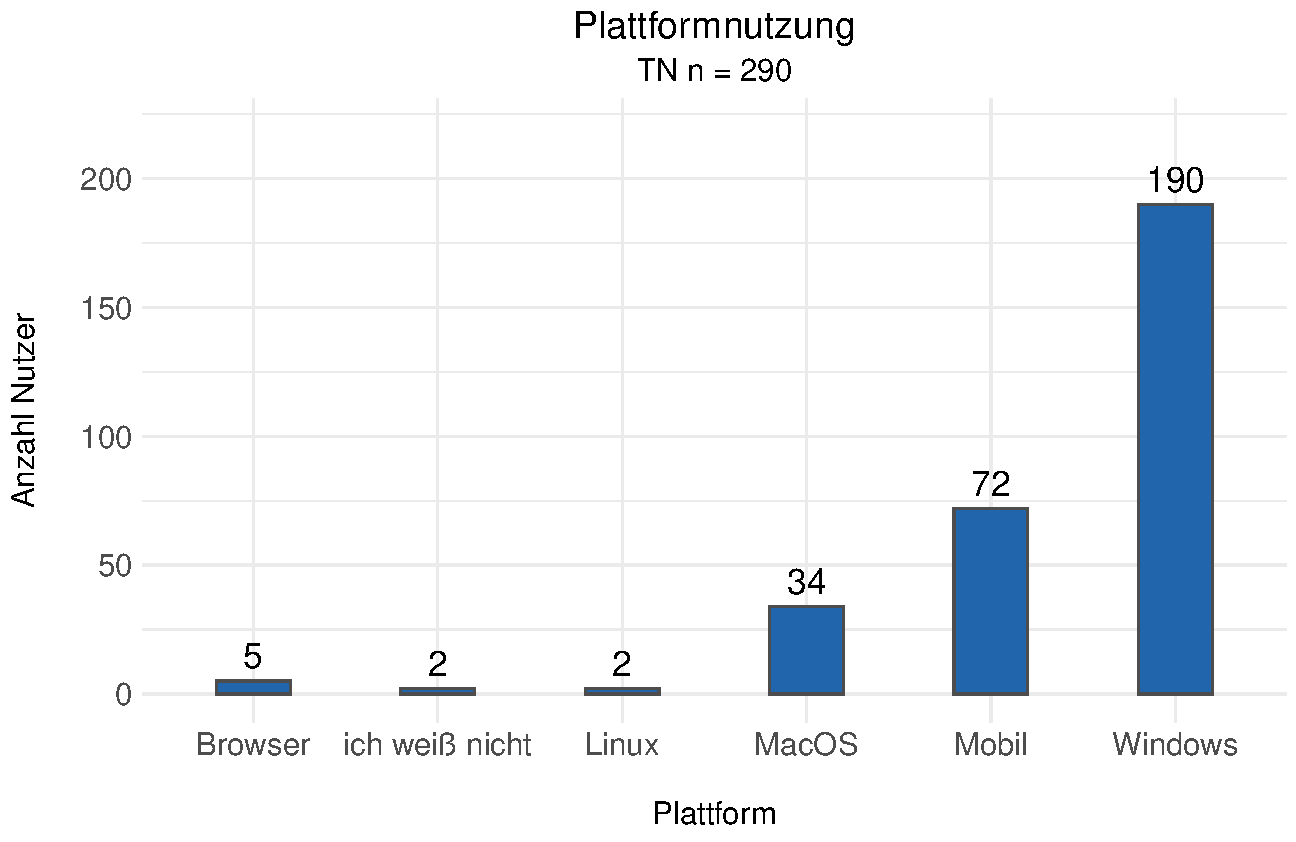
\includegraphics[width=.85\textwidth]{Figures/Umfrage/GGplot/ggplot_skype-plattform_nutzer}
	\caption{Anzahl Nutzer{\textperiodcentered}innen nach Plattform\label{K6:fig:Nutzung-Plattform}}
\end{figure}

% Anzahl Nutzer{\textperiodcentered}innen Funktionen

\begin{figure}[p]
	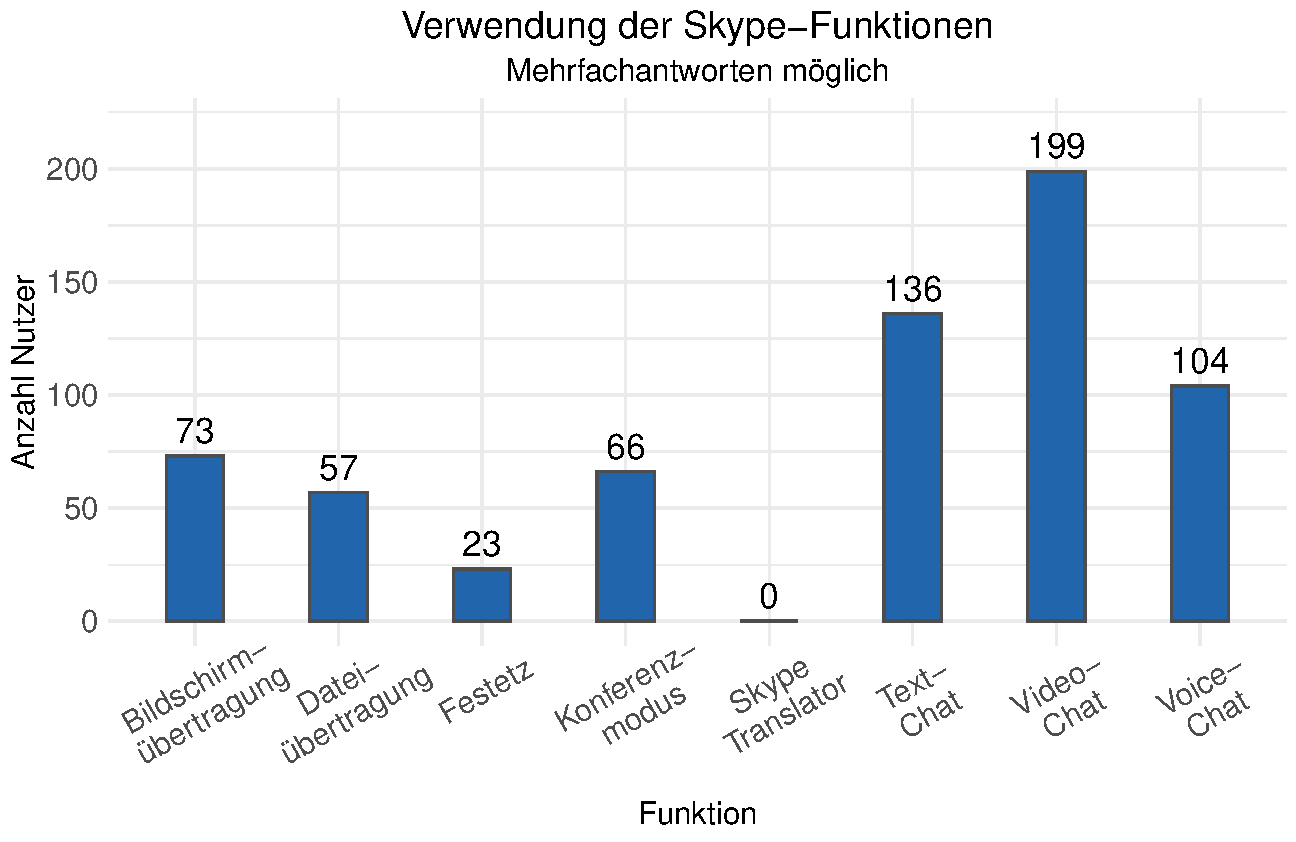
\includegraphics[width=.85\textwidth]{Figures/Umfrage/GGplot/ggplot_skype-funktion_nutzer}
	\caption{Anzahl an Nutzer{\textperiodcentered}innen nach Skype-Funktion}
	\label{K6:fig:Nutzung-Funktionen}
\end{figure}

%------------------------------------------------------------------------

Wie in \figref{K6:fig:Nutzung-Plattform} dargestellt, wurde Skype am häufigsten auf Windows verwendet (190/227, 83,7\,\%). Da bei der Frage nach der Plattform Mehrfachantworten möglich waren, gaben zugleich 72 Teilnehmer{\textperiodcentered}innen (31,7\,\%) an, Skype ebenfalls als mobile Anwendung auf dem Smartphone oder Tablet zu nutzen. 34 Personen (15\,\%) gaben an, den Dienst auf MacOS zu verwenden.\footnote{Diese Frage hat im Verlauf der Ausarbeitung etwas an Relevanz verloren, da der Skype Translator mittlerweile auf allen Plattformen nutzbar ist. Dies war zu Beginn des Forschungsvorhabens 2017 entweder nur begrenzt (MacOS, Browser) oder gar nicht (Linux, Mobil) der Fall.} Dabei nutzten die Teilnehmer{\textperiodcentered}innen vor allem den Video-Chat (199/227, 87,7\,\%) bzw. den Textchat (136/227, 60\,\%) noch vor dem Voice-Chat (104/227, 45,8\,\%).

Die weiteren Funktionen \emph{Bildschirmübertragung}, \emph{Konferenzmodus}, \emph{Dateiübertragung} und \emph{Festnetzanruf} wurden deutlich weniger verwendet, wie in \figref{K6:fig:Nutzung-Funktionen} ersichtlich wird. Auf die Frage, ob der \emph{Skype Translator}\is{Skype!Skype Translator} Verwendung findet, antwortete keine Person mit \emph{Ja}.  Nur drei Personen gaben allgemein an, jemals Erfahrungen mit dem Skype Translator gemacht zu haben.

\begin{sloppypar}
In Bezug auf die Gesprächspartner{\textperiodcentered}innen konnten die Umfrageteilnehmer{\textperiodcentered}\linebreak[3]innen aus acht Kategorien mehrfach auswählen: \emph{Familie}, \emph{Freunde}, \emph{berufliche Zwecke} und \emph{Institutionen}, wobei jede dieser Kategorien noch einmal mit \emph{Inland} und \emph{Ausland} spezifiziert wurde. Besonders häufig sind demnach Freunde im In- und Ausland die Gesprächspartner{\textperiodcentered}innen bei einer Kommunikation über Skype. Jeweils 126 (55,5\,\%) bzw. 143 (63\,\%) Personen gaben dies an. Mehr als ein Drittel der Skypenutzer{\textperiodcentered}innen der Umfrage verwenden den Dienst zudem für Gespräche mit ihrer Familie im In- und Ausland (jeweils 74/227, 32,6\,\%, bzw. 93/227, 41\,\%).
\end{sloppypar}

Deutlich weniger wird Skype für den Kontakt mit Institutionen und für berufliche Zwecke verwendet. Jeweils 43 (18,9\,\%) und 34 (15\,\%) Personen gaben an, den Dienst für berufliche Kontakte im In- und Ausland zu nutzen. Nur 9 (4\,\%) bzw. 5 (2,2\,\%) Personen verwendeten Skype im Umgang mit Institutionen im In- und Ausland.\is{Skype|)}


%------------------------------------------------------

\subsection{Nutzung von Alternativen zu Skype}

\label{K6:sub:Nutzung-Alternativen}

%------------------------------------------------------------------------

\is{Skype!Alternativen zu} Die nachfolgenden Angaben beziehen sich nun wieder auf die eingangs erwähnten 290 vollständigen Datensätze der Umfrageteilnehmer{\textperiodcentered}innen. Mit der Erhebung der verwendeten Alternativen zu Skype begann in der Online-Umfrage ein neuer Block, zu dem die Teilnehmer{\textperiodcentered}innen direkt weitergeleitet wurden, die die Frage nach der generellen Skype-Nutzung verneint hatten.

217 Personen gaben in diesem Teil an, generell Alternativen zu Skype zu verwenden, die ebenfalls einen Voice-, Video- oder Textchat bieten. \figref{K6:fig:NutzungsVgl_Alternativen-Modus} zeigt dabei in Diagramm \emph{A} (linke Seite), wie viele der Teilnehmer{\textperiodcentered}innen die zur Auswahl stehende Alternative nutzen. Diagramm \emph{B} (rechte Seite) zeigt dazu im Vergleich die am häufigsten verwendete Anwendung für den jeweiligen Kommunikationsmodus.

%------------------------------------------------------------------------
% Vergleich Alternativen Nutzung generell vs. häufigste 

\begin{figure}
	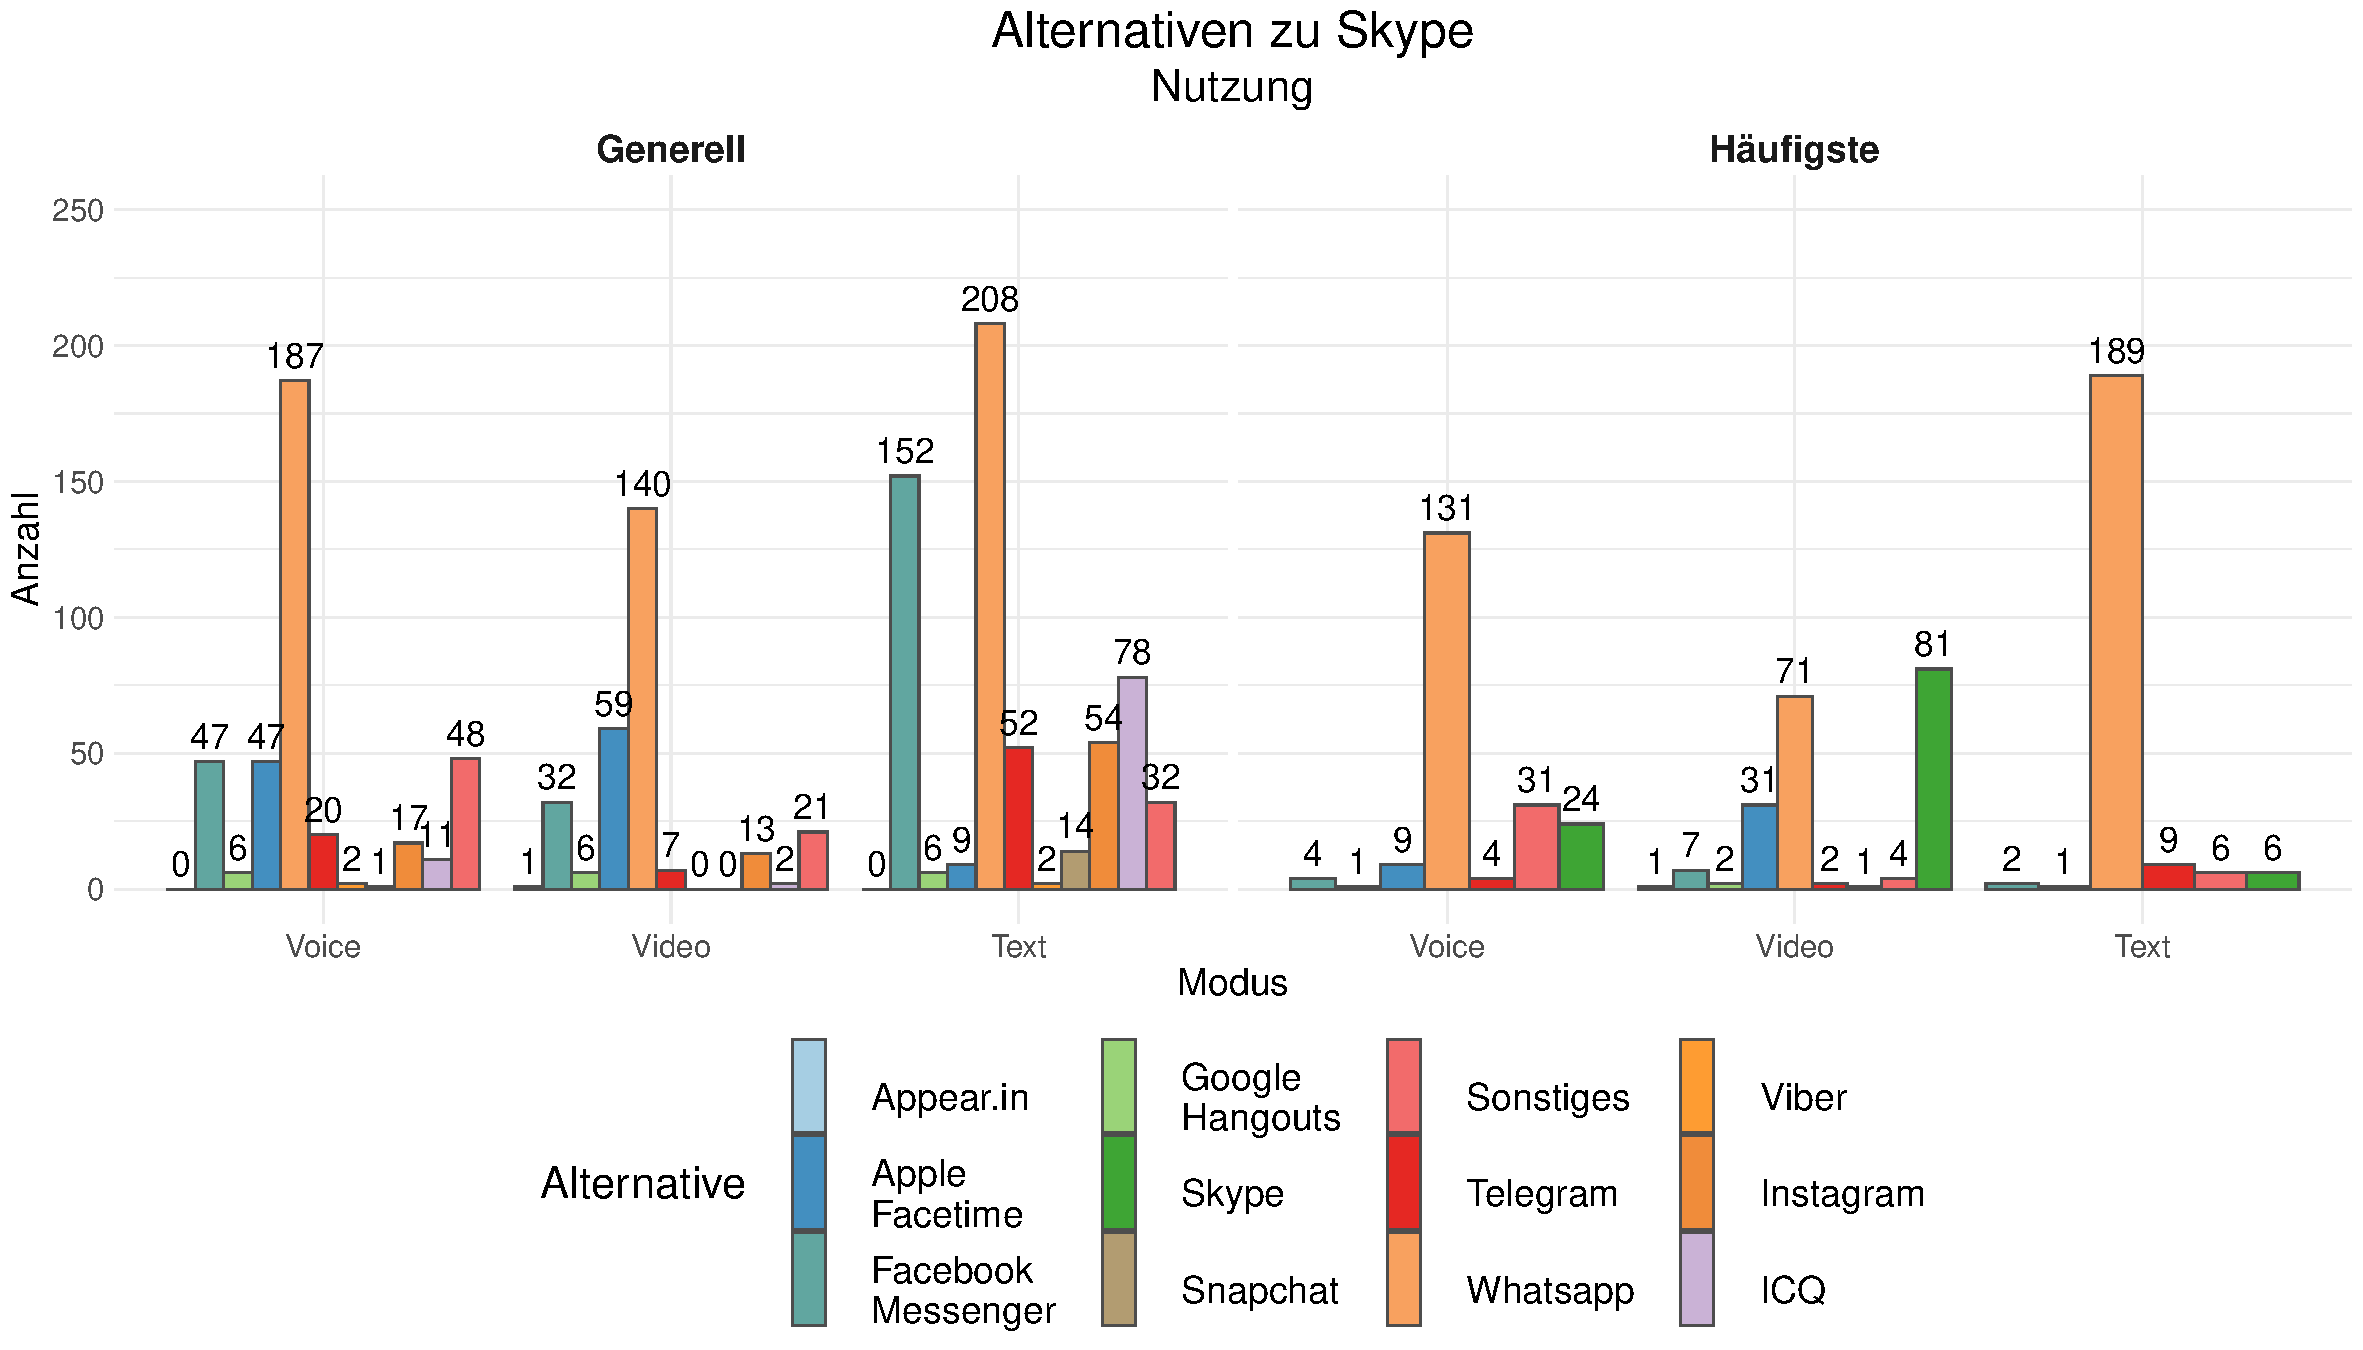
\includegraphics[width=\textwidth]{Figures/Umfrage/GGplot/ggplot_skype_Nutzungsvergleich_Alternativen}
	\caption{Vergleich: Generelle vs. häufigste Nutzung der Alternativen zu Skype nach Modus}
	\label{K6:fig:NutzungsVgl_Alternativen-Modus}
\end{figure}

%------------------------------------------------------------------------

%------------------------------------------------------------------------

\subsection{Situierung der Ergebnisse}
\label{K6:subsec:situierung:allgemeine-Umfrage-SkypeTL}

%------------------------------------------------------------------------

Um die intendierte Gruppe der möglichen Versuchsteilnehmer{\textperiodcentered}innen besser einordnen zu können und einen groben Überblick über das Kommunikationsverhalten\is{Kommunikation!-sverhalten} in der anvisierten Altersgruppe zu erhalten, wurde die in den voranstehenden Abschnitten vorgestellte Online-Umfrage\is{Umfrage!online} konzipiert. Lässt man die in Abschnitt~\ref{K6:subsub:Grundlegendes-Umfrageergebnisse} (S.\,\pageref{K6:subsub:Grundlegendes-Umfrageergebnisse}) angesprochenen auffälligen Altersangaben außer Acht, so ergibt sich ein überwiegend weibliches und junges, sich in den Zwanzigern befindliches Feld an Teilnehmer{\textperiodcentered}innen. Die meisten der Umfrageteilnehmer{\textperiodcentered}innen besitzen mindestens die Hochschulzugangsberechtigung oder sogar bereits einen ersten akademischen Abschluss. Die Kerngruppe kann daher als formal gut gebildet definiert werden. Die Mehrheit der Umfrageteilnehmer{\textperiodcentered}innen gibt Deutsch als Muttersprache an, auch wenn häufig noch mindestens eine weitere, wenn nicht sogar zwei oder mehr Sprachen genannt werden. Insgesamt werden 36 verschiedene Sprachen aufgeführt.

Skype\is{Skype|(} wird generell selten (mehrheitlich monatlich und seltener als monatlich), aber dafür lange (länger als eine Stunde oder mindestens eine Stunde) genutzt. Das häufigste Betriebsystem, auf dem Skype genutzt wird, ist Windows, auch wenn ein Drittel der Teilnehmer{\textperiodcentered}innen darüber hinaus auch noch die App für das Smartphone verwendet. Die meistgenutzte Funktion von Skype ist der Videochat.\is{Chat!Video-} Die Gesprächspartner{\textperiodcentered}innen sind überwiegend Freunde im In- und Ausland. Allerdings geben die Befragten mehrheitlich an, parallel dazu auch Alternativen zu Skype zu verwenden. Für den Voice-\is{Chat!Voice-}, Video-\is{Chat!Video-} und Textchat\is{Chat!Text-} ist dies WhatsApp\is{WhatsApp}. Ebenfalls häufig wird für Textnachrichten der Facebook Messenger\is{Facebook!Messenger}\is{Facebook Messenger|see{Facebook}} genutzt. Die jeweils am meisten genutzte Software für die jeweilige Funktion ist für Voice- und Textchats WhatsApp, für Videochats Skype.

Die Nutzungsangaben in der Umfrage decken sich mit repräsentativen Erhebungen zum Kommunikationsverhalten\is{Kommunikation!-sverhalten} und zur Mediennutzung der vergangenen Jahre. So kam eine von Deloitte durchgeführte Studie \citep[]{deloitte_nutzung_2017} zur Nutzung von Messaging-Diesten nach Altersgruppen aus dem Jahre 2017 zu dem Ergebnis, dass jeweils über 80\,\% der 18--24-Jährigen und 25--34-Jährigen \emph{Mobile Instant Messaging} nutzt. Andere Antwortmöglichkeiten wie E-Mail, \emph{Social Network Messaging} oder SMS fallen hinter diesem Ergebnis deutlich zurück. In diesem Zusammenhang ergibt die Studie zudem, dass über den Zeitraum von 2013 bis 2018 die Nutzung von Mobile Instant Messaging, E-Mail und Social Network zugenommen hat. Die Nutzung von SMS hingegen ging zurück \citep[]{deloitte_top_2019}\is{Skype|)}.

\begin{sloppypar}
Laut einer von Bitkom durchgeführten Erhebung zur primär verwendeten Mes\-sen\-ger-App von August 2018 nutzen über 80\,\% der Befragten vor allem WhatsApp\is{WhatsApp}. An zweiter Stelle mit 42\,\% steht der Facebook Messenger\is{Facebook!Messenger} noch vor Skype mit 22\,\%. Dieselbe Studie erhebt weiterhin die meistgenutzten Funktionen bei Messenger-Apps. Die Teilnehmer{\textperiodcentered}innen geben hierbei an, vor allem Nachrichten zu schreiben (82\,\%) und Bilder, Videos u.ä. Inhalte zu versenden (70\,\%). Telefonie und Videochats werden erst an dritter (50\,\%) bzw. sechster Stelle (27\,\%) genannt. Eine Auswahl der App nach der internationalen Verfügbarkeit ist den Umfrageteilnehmer{\textperiodcentered}innen dabei weniger wichtig \citep[]{joachim_thommes_grose_2018}.
\end{sloppypar}

%------------------------------------------------------------------------

\section{Die Proband{\textperiodcentered}innen im Setting Katalanisch-Deutsch}
\label{K6:sec:Probandinnen-CatDe}

%------------------------------------------------------------------------

%%%%%%%%%%%%%%%%%%%%%%%%%%%%%%%
%!!!!!!!!
% Brillen-/Kontaktlinsenträger miteinbeziehen wegen möglicher Verfälschung der Messergebnisse


Als Zielgruppe für die Studie wurden eingeschriebene Student{\textperiodcentered}innen der Leipziger Hochschulen ungeachtet des Studiengangs erachtet. Als eine für dieses Experiment hinreichend große Gruppe wurde eine Anzahl von 15--20 Proband{\textperiodcentered}innen erachtet. Zwei Ausschlusskriterien mussten mögliche Teilnehmer{\textperiodcentered}innen zwingend erfüllen: Sie sollten über keine, allenfalls wenige (max. Niveau A gem. Europ. Referenzrahmen), Katalanischkenntnisse verfügen und Deutsch als Muttersprache ansehen. Ein Studienaufruf wurde an die Studierendenvertretung der Universität Leipzig und der HTWK gesendet. Die Vergütung bestand aus einer Aufwandsentschädigung von 10 Euro.

Als katalanischsprachige Gesprächspartner{\textperiodcentered}innen fungierten drei Frauen und ein Mann aus unterschiedlichen Gebieten der katalanischsprachigen Länder (\emph{paisos catalans}) -- aus Valencia, Girona und Barcelona. Die Personen waren jeweils 26, 24, 25 und 26 Jahre alt. Weiterhin wiesen alle vier Personen Deutschkenntnisse durch einen studienbedingten Aufenthalt in Deutschland auf. Die katalanischen Muttersprachler{\textperiodcentered}innen erhielten jedoch weder den Fragebogen vor oder nach dem Experiment, noch wurden sie selbst okulometrisch erfasst.

Auch wenn der Einsatz einer einzigen katalanischsprachigen Person als Gesprächspartner{\textperiodcentered}in die Vergleichbarkeit der Daten untereinander sicherlich erhöht hätte, wurde von dieser Möglichkeit bewusst abgesehen. Bereits in der Pilotierungsphase\is{Pilotierung} hatte sich herausgestellt, dass die Koordination einer Studie, die von der gleichzeitigen Verfügbarkeit zweier Personen (jeweils Proband{\textperiodcentered}in und Gesprächspartner{\textperiodcentered}in) sowie vom Zugang zum Eye-Tracker\is{Eye-Tracking} abhängt, ein kommunikationsintensives Vorhaben wird. Um den Versuchsteilnehmer{\textperiodcentered}innen möglichst viel Spielraum bei der Terminfindung zu bieten und so den unnötigen Wegfall von potenziellen Proband{\textperiodcentered}innen aus Termingründen zu vermeiden, wurden mehrere katalanische Gesprächspartner{\textperiodcentered}innen rekrutiert.

Insgesamt wurde das Experiment, beginnend mit der Einweisung und dem Fragebogen, über die Kommunikationssituation\is{Kommunikation!-ssituation} bis hin zum abschließenden Fragebogen\is{Fragebogen} und Debriefing\is{Debriefing}, auf eine Länge von 60 Minuten pro Proband{\textperiodcentered}in ausgelegt, wobei die Gesprächssituation sich auf etwa 15 Minuten beschränken sollte. Um den Studienteilnehmer{\textperiodcentered}innen nicht gänzlich unvorbereitet in eine derartige Situation hineinzuwerfen und um mit Blick auf die Weiterverwendung der gewonnenen Sprachdaten eine einheitliche Ausgangssituation zu schaffen, wurde ein generelles Gesprächsthema angekündigt: Die Proband{\textperiodcentered}innen sollten so tun, als bereiteten sie sich auf ein Auslandssemester in der Heimatstadt des katalanischen Gegenübers vor. Um Informationen zur Wohnungssuche (und zur Universität usw.) zu erhalten, kontaktierten sie deshalb die jeweilige Person.

Im Zeitraum zwischen Februar und Dezember 2019 wurde die Studie im Setting Katalanisch-Deutsch mit 25 Personen durchgeführt. Vier der dabei erhaltenen Datensätze wurden jedoch im Zuge der Datensichtung aufgrund von entweder schlechter Aufnahmequalität oder technischen Problemen bei der Aufnahme ausgeschlossen. So ergibt sich eine Kohorte von 21 Personen: 13 Frauen und acht Männer im Alter von 20 bis 32 Jahren (\diameter\,23,7 Jahre, Median = 23 Jahre, SD = 4,0).

Zwei der teilnehmenden Student{\textperiodcentered}innen gaben an, die Hochschulzugangsberechtigung und eine abgeschlossene Ausbildung zu besitzen, eine weitere Person konnte sowohl die allgemeine Hochschulreife als auch eine abgeschlossene Ausbildung vorweisen. Bis auf eine Person von der HTWK kamen alle Teilnehmer{\textperiodcentered}innen von der Universität Leipzig und waren zum Zeitpunkt der Erhebung regulär eingeschrieben. 

Die Studienfächer der Proband{\textperiodcentered}innen sind in \tabref{K6:tab:Fach_TN-Feldstudie-CatDe} und die Fachsemesteranzahl in \tabref{K6:tab:Semester_TN-Feldstudie-CatDe} aufgeschlüsselt. Studierende des Instituts für Angewandte Linguistik und Translatologie durften ebenfalls an der Studie teilnehmen, sofern Sie explizit keinerlei Vorkenntnisse im Katalanischen besaßen.


%------------------------------------------------------------------------

\begin{table}
	\begin{tabular}{lccc}
	\lsptoprule
		& {Bachelor} & {Master} & {Staatsexamen}\\ 
	\midrule
		Konferenzdolmetschen & - & 1 & - \\ 
		Übersetzen & 1 & 0 & -\\ 
		Lehramt & - & - & 5 \\ 
		Interkult. Komm. & 1 & 0 & - \\ 
		BWL & 1 & 0 & - \\ 
		Medizin & - & - & 5 \\ 
		DaF/DaZ & 3 & 1 & - \\ 
		Linguistik & 3 & 0 & -\\\midrule
		{gesamt} & 9 & 2 & 10\\\cmidrule(lr){2-4}
		& \multicolumn{3}{c}{21} \\ 
	\lspbottomrule
	\end{tabular}
	\caption{Studienfächer der Teilnehmer{\textperiodcentered}innen\label{K6:tab:Fach_TN-Feldstudie-CatDe}}
\end{table}
%------------------------------------------------------------------------

%------------------------------------------------------------------------
\begin{table}
    
    \begin{tabular}{lcccccccccccc}
	\lsptoprule
		{Fachsemester} & {1} & {2} & {3} & {4} & {5} & {6} & {7} & {8} & {9} & {10} & {11}\\ 
	\midrule
		Konferenzdolmetschen & - & - & - & - & - & - & 1 & - & - & - & - \\ 
		Übersetzen & - & - & - & - & - & - & 1 & - & - & - & - \\ 
		Lehramt & 2 & - & - & 1 & - & 1 & - & 1 & - & - & - \\ 
		Interkult. Komm. & - & - & 1 & - & - & - & - & - & - & - & - \\ 
		BWL & - & - & - & - & - & 1 & - & - & - & - & - \\
		Medizin & - & - & - & 1 & - & 2 & - & 1 & - & - & 1 \\ 
		DaF/DaZ & 1 & - & 2 & - & - & 1 & - & - & - & - & - \\ 
		Linguistik & - & - & - & - & 3 & - & - & - & - & - & - \\ 
	\lspbottomrule
	\end{tabular}
	\caption{Fachemester der Teilnehmer{\textperiodcentered}innen\label{K6:tab:Semester_TN-Feldstudie-CatDe}}
\end{table}
%------------------------------------------------------------------------

Auf die Frage nach der Sprache, mit der die Proband{\textperiodcentered}innen primär aufgewachsen seien, gaben alle Personen Deutsch an. Jeweils eine Person gab darüber hinaus noch Russisch oder Englisch an, eine weitere sowohl Russisch als auch Englisch. 

Die hauptsächlich im Alltag und im Beruf verwendete Sprache war für alle Teilnehmer{\textperiodcentered}innen Deutsch, wobei zwei Proband{\textperiodcentered}innen sich der Frage nach der Berufssprache enthielten. Als weitere Fremdsprachen gaben die Proband{\textperiodcentered}innen überwiegend Englisch an (17/21). Weitere Sprachen können \figref{K6:fig:Fremdspr-Prob-CatDe} entnommen werden, wobei auch hier wieder eine Mehrfachnennung möglich war.
  

%------------------------------------------------------------------------

\begin{figure}
	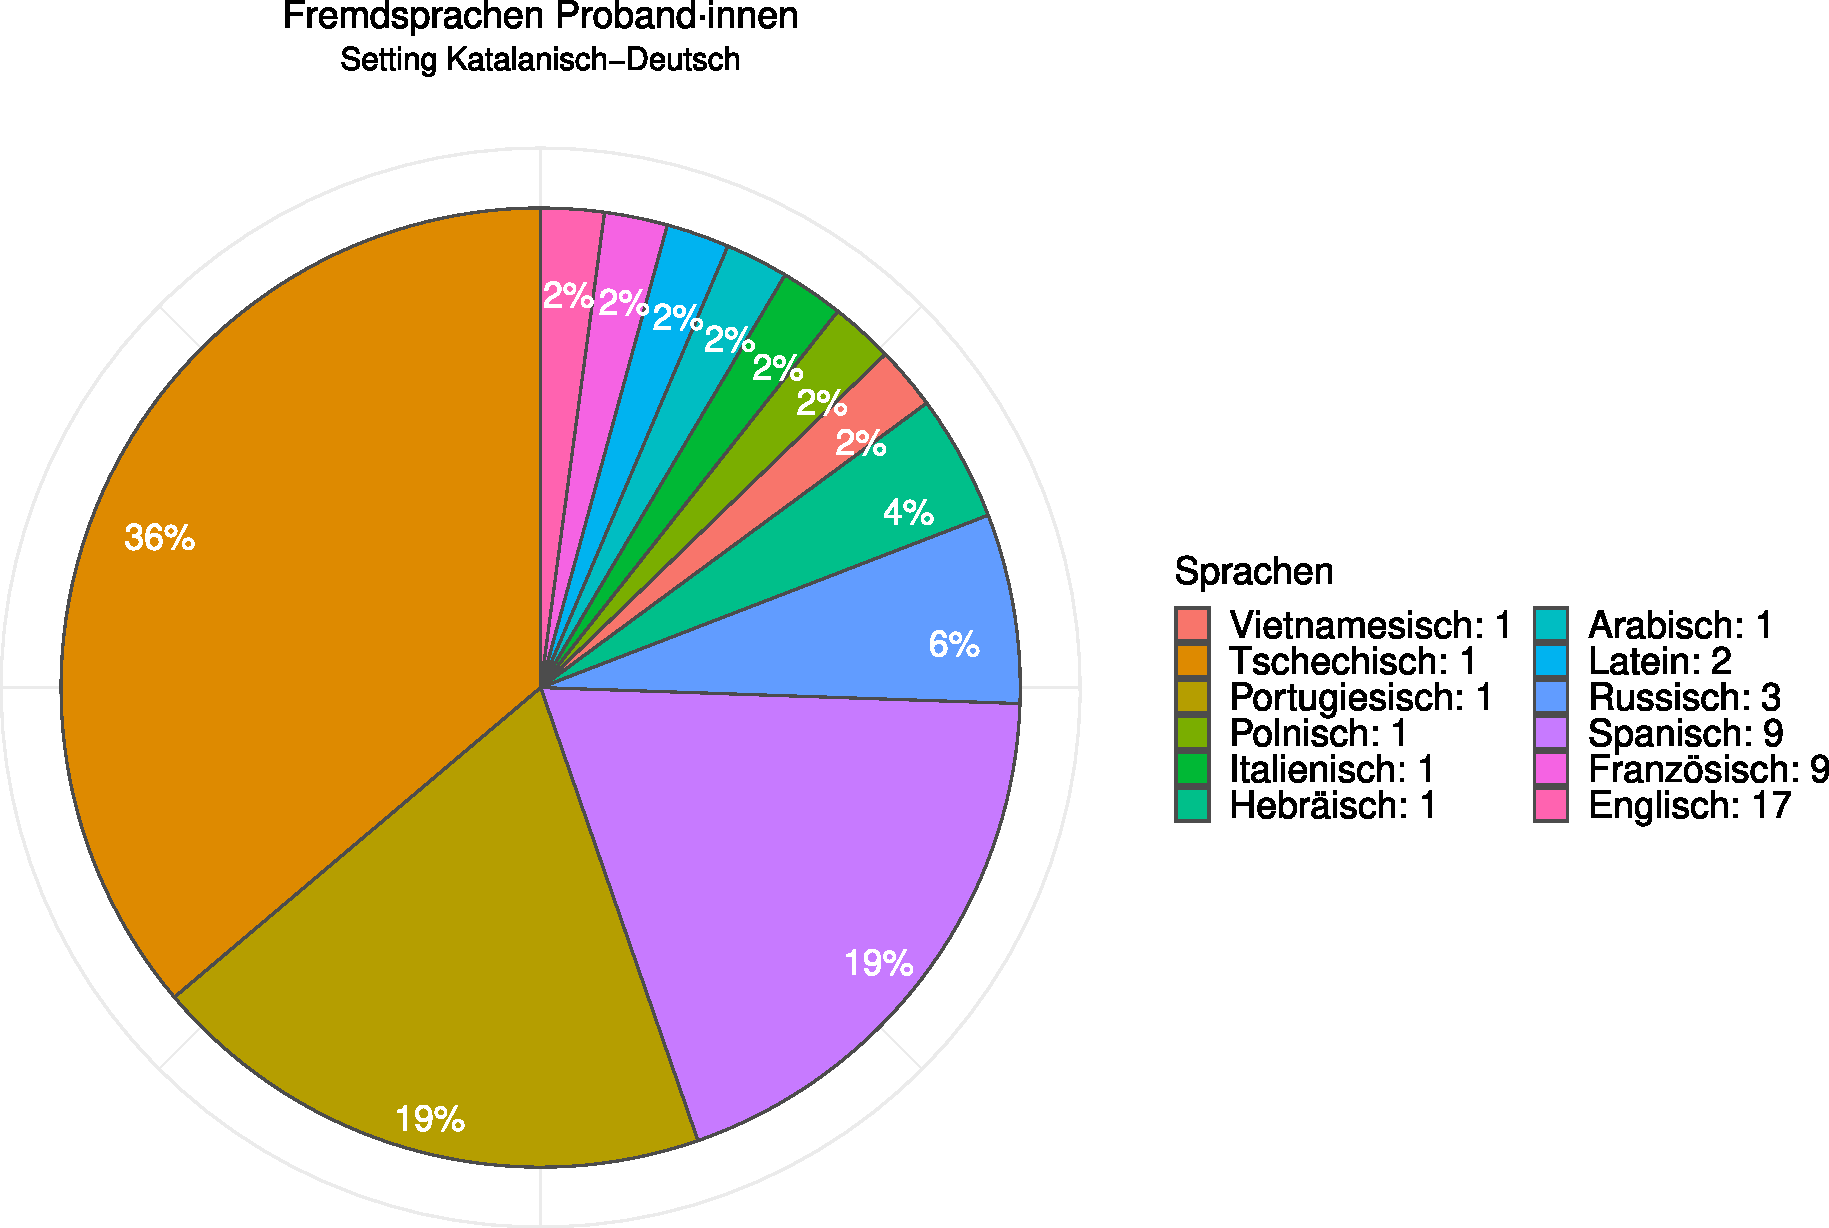
\includegraphics[width=\textwidth]{Figures/EingangsFB/ggplot_sprachen_CatDe_probanden}
	\caption{Fremdsprachen der Proband{\textperiodcentered}innen}
    \label{K6:fig:Fremdspr-Prob-CatDe}
\end{figure}

%------------------------------------------------------------------------


%------------------------------------------------------------------------

\begin{figure}
    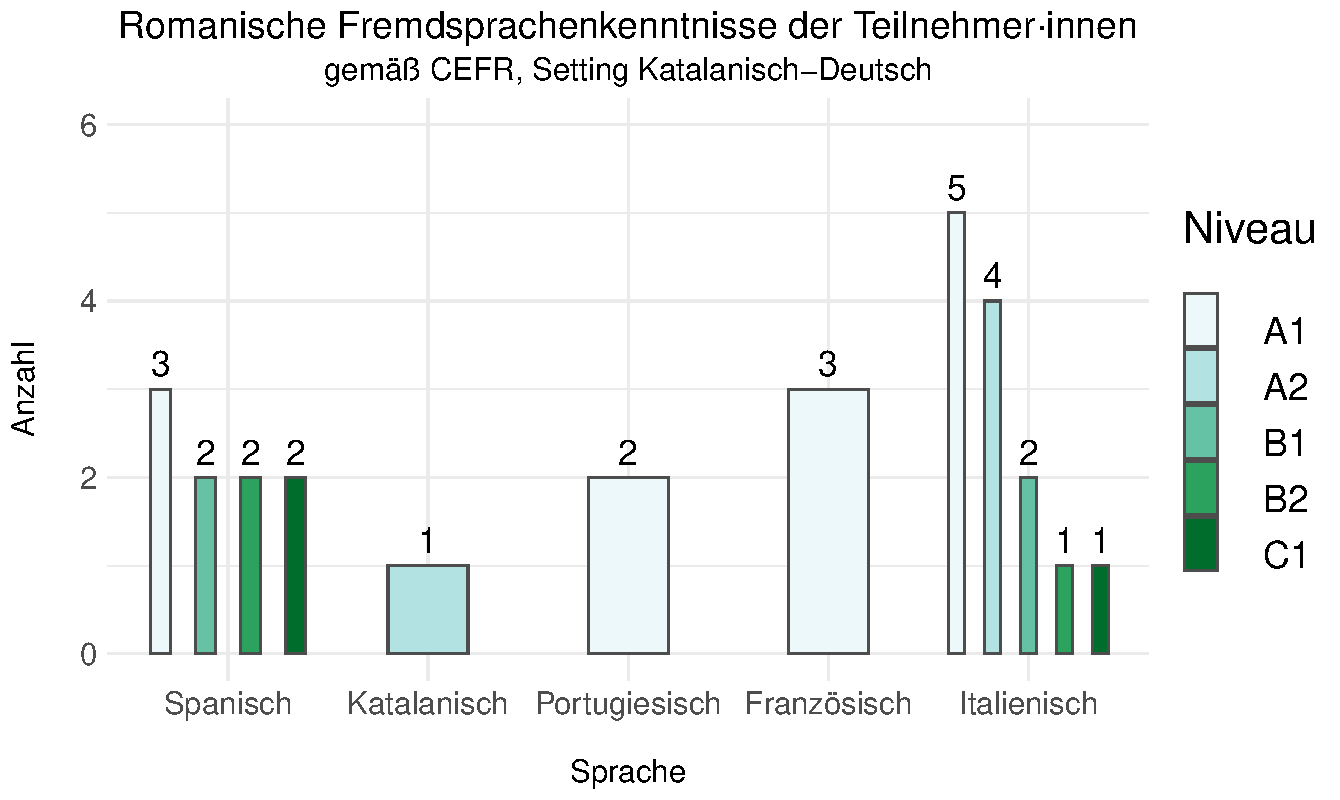
\includegraphics[width=\textwidth]{Figures/EingangsFB/ggplot_Fremdsprachen-CEFR-CatDe}
	\caption{Kompetenz in ausgewählten romanischen Sprachen\label{K6:fig:CEFR-Niveau-CatDe}}
\end{figure}

%------------------------------------------------------------------------



%------------------------------------------------------------------------

\subsection{Angaben der Proband{\textperiodcentered}innen im Eingangsfragebogen}
\label{K6:subsec:Angaben-Eingang-Probandinnen-CatDe}

%------------------------------------------------------------------------

Zu Beginn der Erhebung, vor der Textchatkommunikation\is{Kommunikation!Chat-}\is{Chat!-kommunikation}\is{Chat!Text-} über Skype, wurden die Teilnehmer{\textperiodcentered}innen gebeten, einen Eingangsfragebogen\is{Fragebogen!Eingangs-} auszufüllen. Die Angaben in diesem Fragebogen dienen der Verortung der Kohorte in Bezug auf Nutzungsverhalten derartiger Kommunikationssoftware.

Von den 21 Studienteilnehmer{\textperiodcentered}innen gaben 17 an, Skype\is{Skype!Nutzung von} zu nutzen. Die weiteren vier Teilnehmer{\textperiodcentered}innen erhielten daher nicht den Fragenteil zum Nutzungsverhalten, sondern nur zur Auslandserfahrung und Fremdsprachenbeherrschung sowie die demographischen Angaben. Deshalb wird im Folgenden zunächst nur von 17 Proband{\textperiodcentered}innen ausgegangen. Von diesen 17 verwendeten 15 Skype seltener als monatlich, eine Person monatlich und eine wöchentlich. In Bezug auf die Nutzungsdauer pro Sitzung gaben fünf an, die Anwendung bis zu 15 Minuten zu nutzen, weitere fünf bis zu 30 Minuten, drei bis zu einer Stunde und vier länger als eine Stunde. 14 Personen gaben an, Skype für Windows zu verwenden, jeweils eine für MacOS und im Browser und sechs als mobile App. Bei dieser Frage waren Mehrfachantworten möglich.

Die Mehrheit der Proband{\textperiodcentered}innen nutzte Skype für Video-\is{Chat!Video-} (15/17) oder Textchats\is{Chat!Text-} (11/17), wohingegen der Voice-Chat\is{Chat!Voice-} von nur vier Proband{\textperiodcentered}innen genutzt wurde. Auch die weiteren Funktionen wurden nur von wenigen Studienteilnehmer{\textperiodcentered}innen verwendet: Festnetzanruf (3/17), Bildschirmübertragung (4/17), Konferenzmodus (5/17), Dateiübertragung (4/17). Der Skype Translator\is{Skype!Skype Translator} wurde von niemandem genutzt. Auch bei dieser Frage waren Mehrfachantworten möglich.

\begin{sloppypar}
Die Proband{\textperiodcentered}innen geben ihre Erfahrungen in Bezug auf den Textchat\is{Chat!Text-} durchweg mit gut (11/17) bzw. überwiegend gut (3/17) an, wobei sich die verbleibenden Teilnehmer{\textperiodcentered}innen der Antwort enthielten. Sowohl die Videochat-\is{Chat!Video-} als auch die Voicechat-Funktion\is{Chat!Voice-} werden hingegen etwas schlechter wahrgenommen: Zwei Proband{\textperiodcentered}innen haben gute Erfahrungen mit der Videoübertragung gemacht, zehn waren der Ansicht, die Übertragung sei überwiegend gut und fünf empfanden sie als eher schlecht. Der Voicechat wurde nur von einer Person als gut empfunden, zehn bewerteten ihn überwiegend gut und zwei eher schlecht.
\end{sloppypar}

In puncto Gesprächspartner{\textperiodcentered}innen gaben fünf der Proband{\textperiodcentered}innen an, mit Familienmitgliedern im Inland und zehn mit Familienmitgliedern im Ausland zu kommunizieren. Acht verwendeten Skype für die Kommunikation\is{Kommunikation!-spartner{\textperiodcentered}in} mit Freunden im Inland, 12 für den Kontakt mit Freunden im Ausland. Lediglich zwei bzw. eine Person gaben an, Skype\is{Skype} für berufliche Zwecke im In- bzw. Ausland zu nutzen. Eine Person gab an, Skype sowohl für die Kommunikation mit Institutionen im In- und Ausland zu verwenden. Die häufigste Sprache, die neben Deutsch (17/17) in diesen Situationen verwendet wurde, ist Englisch (8/17). Weiterhin wurden Russisch (3/17), Spanisch (2/17), Franzöisch (1/17) und Ungarisch (1/17) angegeben. Auch bei diesem Fragenteil waren Mehrfachantworten möglich.

13 der 21 Proband{\textperiodcentered}innen gaben weiterhin an, bereits längere Zeit (mehr als vier Wochen Minimum, kein Urlaub) im Ausland verbracht zu haben. Die bereisten Länder der Teilnehmer{\textperiodcentered}innen verteilen sich über die gesamte Erde, wobei ein Schwerpunkt auf Europa auszumachen ist. Sieben Versuchsteilnehmer{\textperiodcentered}innen gaben zwei oder mehr Länder an, in denen sie mehr als vier Wochen verbracht haben. Die in den jeweiligen Ländern verbrachte Dauer reicht von einem bis 110 Monate (9,17 Jahre, \diameter\,30,5 Monate, Median = 16 Monate, SD = 37,85). Als Gründe wurden Spracherwerb (7/21), Sprachvertiefung (7/21), Kulturkontakt (11/21), ein Pflichtaufenthalt (1/21), eine Fortbildung (1/21), berufliche Motive (2/21) sowie die (zeitweise) Verlagerung des Lebensmittelpunktes (3/21) genannt. Dabei lagen die Aufenthalte zwischen drei und 166 Monaten zurück (entspricht 13,83 Jahren, \diameter\,34,2 Monate, Median = 16 Monate, SD = 49,9).

%------------------------------------------------------

\subsection{Nutzung von Alternativen zu Skype}

\label{K6:subsubsec:Nutzung-Alternativen-CatDe}

%------------------------------------------------------------------------

\is{Skype!Alternativen zu|(}Im Folgenden beziehen sich die Angaben zur Nutzung von Alternativen zu Skype nun wieder auf alle 21 Studienteilnehmer{\textperiodcentered}innen. Analog zu den Ergebnissen der Online-Umfrage\is{Umfrage!online} gaben auch die Proband{\textperiodcentered}innen der Studie an, bislang keine Erfahrungen mit dem Skype Translator\is{Skype!Skype Translator} gemacht zu haben. Wohlwollend interpretiert, könnte dies als favorable Ausgangslage angesehen werden, da so keine Beeinträchtigungen durch Vorerfahrung in die Studie einfließen. Andererseits jedoch zeichnet sich ein recht unpopuläres Gesamtbild des Features ab.

17 Teilnehmer{\textperiodcentered}innen gaben an, generell Software zu verwenden, die ebenfalls eine Voice-\is{Chat!Voice-} oder Videochat-Funktion\is{Chat!Video-} bietet. Sowohl in Hinblick auf Voice- als auch auf den Videochat gab die Mehrheit an, WhatsApp\is{WhatsApp} zu verwenden (jeweils 17 bzw. 14/21). Die anderen angebotenen Alternativen in dieser Frage (s. Frage im Anhang~\ref{App2:Alternativen-generell}, S.\,\pageref{App2:Alternativen-generell}) wurden allesamt stets von weniger als sieben Proband{\textperiodcentered}innen überhaupt verwendet. Beim Textchat\is{Chat!Text-} wurden sowohl der Facebook Messenger als auch WhatsApp als generelle Alternative zu Skype angegeben (jeweils 14 bzw. 16/21). Auch hier erhielten die anderen angebotenen Alternativen nie mehr als sechs Angaben. Im Vergleich dazu gaben die Proband{\textperiodcentered}innen antworteten auf die Frage nach dem Dienst, der für Voice-\is{Chat!Voice-}, Video-\is{Chat!Video-} und Textchat\is{Chat!Text-} jeweils am Häufigsten verwendet wird, deutlich diverser.

Die für Videochats\is{Chat!Video-} am häufigsten verwendeten Dienste sind demnach WhatsApp (7/21), Skype (3/21), Facebook Messenger sowie Apple Facetime (jeweils 2/21) bzw. Discord (1/21). Auch bei Voice-Chats\is{Chat!Voice-} wurde WhatsApp am häufigsten verwendet (11/21). Ebenfalls wurden Facebook Messenger (2/21), Discord (2/21), Viber (1/21) sowie das Haustelefon (1/21) genannt. Gleichermaßen ist WhatsApp ebenso bei Textchats\is{Chat!Text-} die am häufigsten verwendete Alternative (15/21), bei jeweils einer Nennung von Facebook Messenger und Google Hangouts.
\is{Skype!Alternativen zu|)}

%------------------------------------------------------------------------

\begin{figure}
    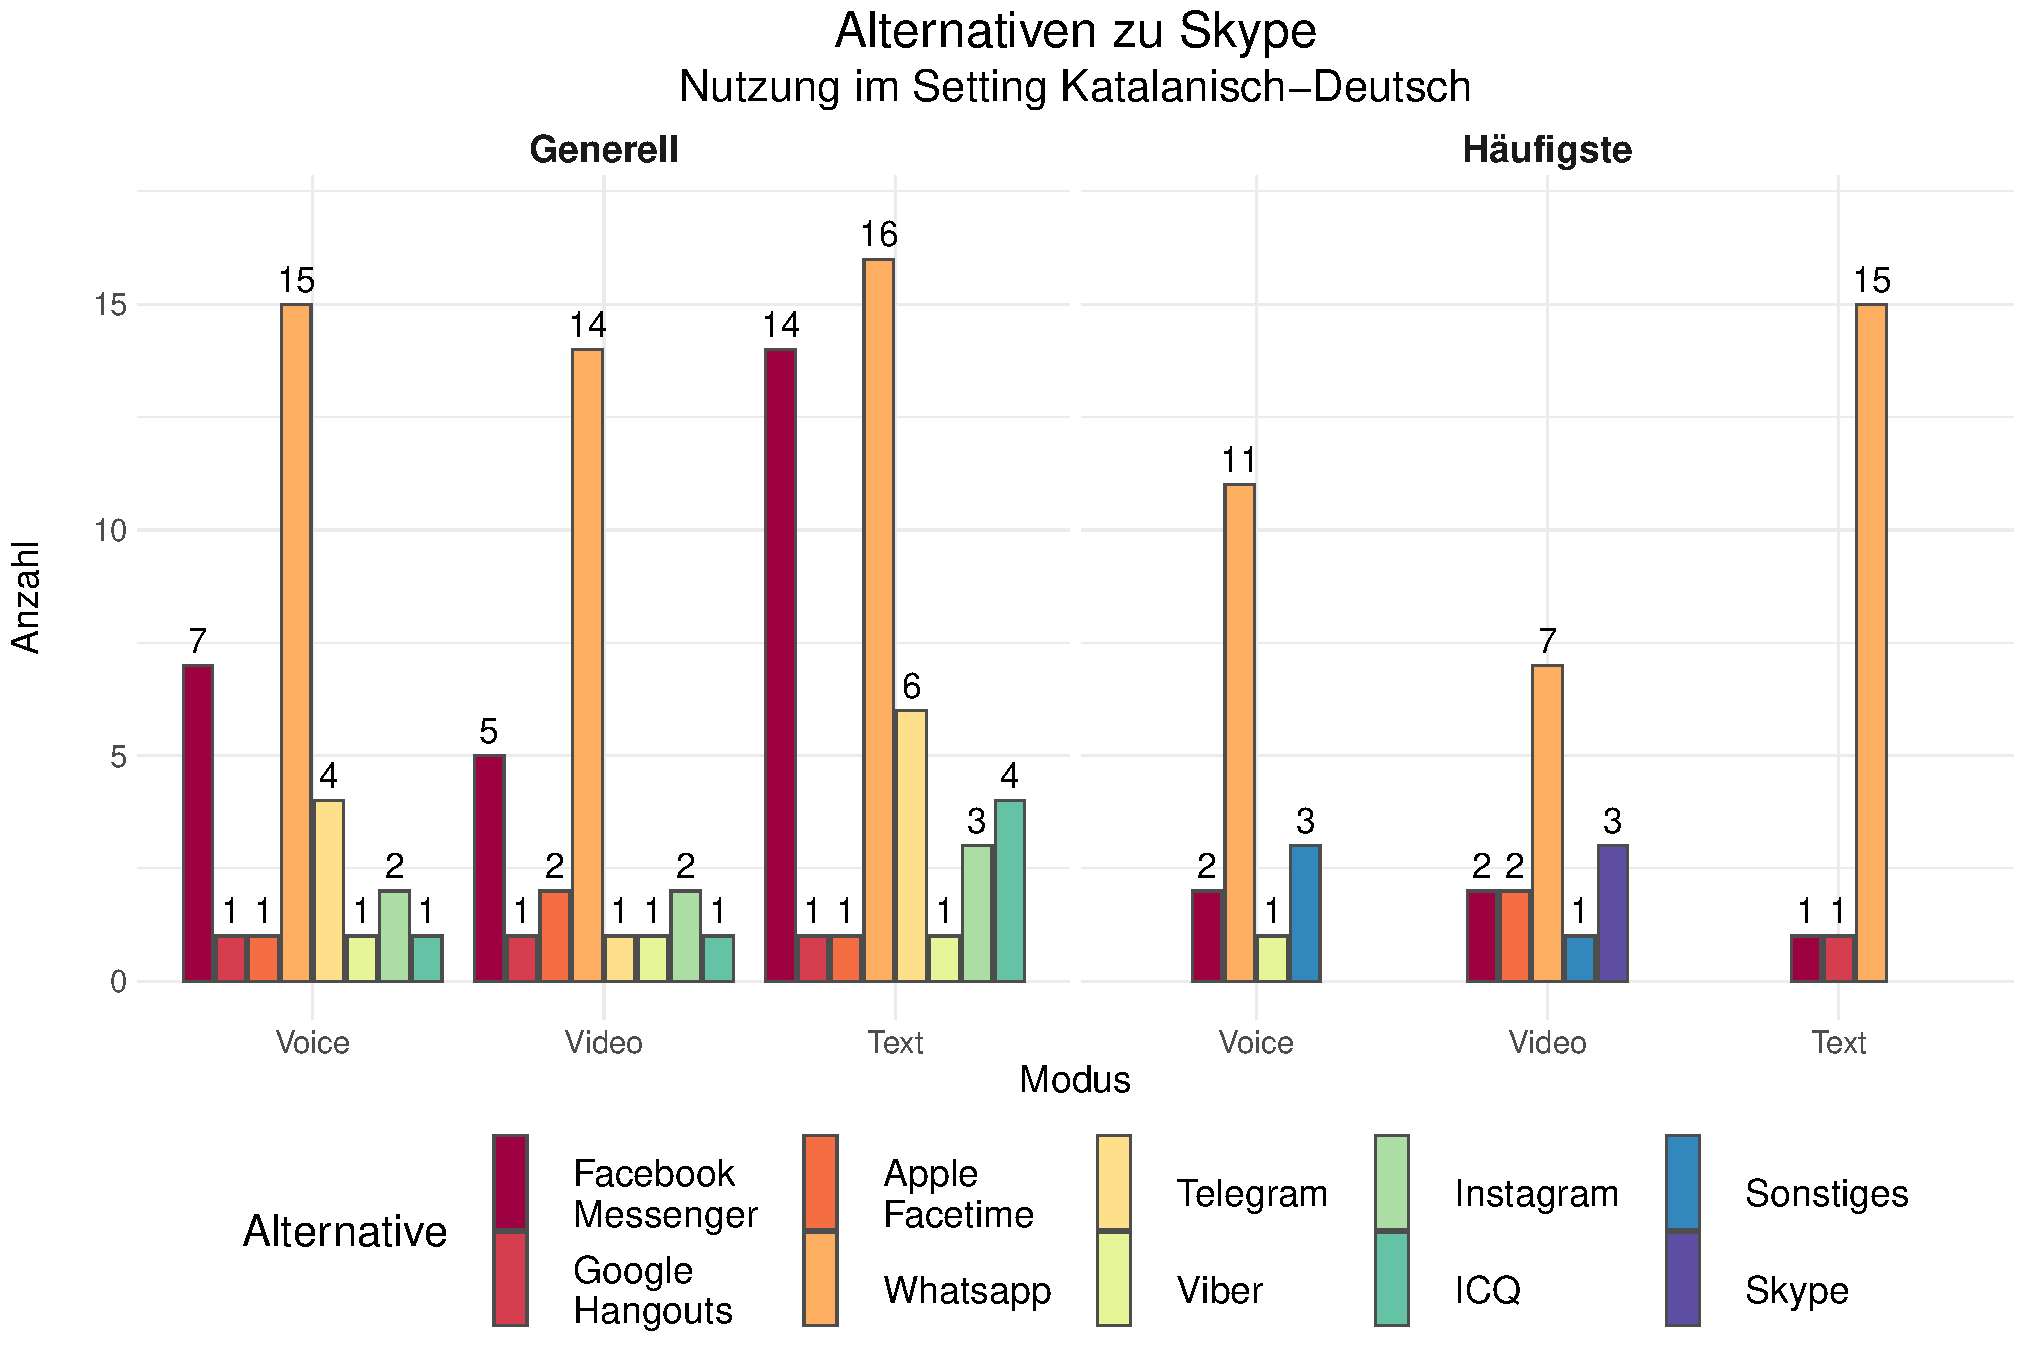
\includegraphics[width=\textwidth]{Figures/EingangsFB/ggplot_skype_Nutzungsvergleich_Alternativen-CatDe}
	\caption{Vergleich Generelle und häufigste Nutzung der Alternativen zu Skype nach Modus}
    \label{K6:fig:NutzungsVgl-Alternativen-Modus-CatDe}
\end{figure}

%------------------------------------------------------------------------

%------------------------------------------------------------------------

\subsection{Angaben der Proband{\textperiodcentered}innen im Ausgangsfragebogen}

\label{K6:sub:Ausgangsfragebogen:CatDe}

%------------------------------------------------------------------------
\begin{sloppypar}
Unmittelbar nach Beendigung der Eye-Tracking-Sitzung\is{Eye-Tracking} wurden die Proband{\textperiodcentered}\linebreak[3]innen gebeten, den Ausgangsfragebogen\is{Fragebogen!Ausgangs-} auszufüllen (s. Anhang \ref{App3:GB}, S.\,\pageref{App3:GB}\,ff.). Zweck dieses Fragebogens war es, die unmittelbare Einschätzung der Studienteilnehmer{\textperiodcentered}innen zur gerade erlebten Kommunikationssituation\is{Kommunikation!-ssituation} unter Beteiligung des Skype Translators\is{Skype!Skype Translator} zu erfassen. Auch an diesem Teil der Erhebung nahmen alle 21 Personen teil. Die Teilnahmebedingungen waren die gleichen wie auch beim Eingangsfragebogen (zum datenschutzrechtlichen Hinweis s. Anhang~\ref{App2:Alternativen-generell}, S.\,\pageref{App2:EinweisungEva}).
\end{sloppypar}

Zunächst wurde um eine generelle Einschätzung der Aspekte \emph{Gesprächsqualität}, \emph{Übersetzungsqualität} und \emph{Versuchsaufbau} gebeten. Die Aspekte \emph{Tonqualität} sowie \emph{Videoqualität} wurden vernachlässigt, da die Kommunikationssituation\is{Kommunikation!-ssituation} im Modus Textchat stattfand. Dies geschah durch eine vorangestellte Ja-Nein-Frage, zu welchen Aspekten die Teilnehmer{\textperiodcentered}innen sich in der Lage sahen, eine Einschätzung abzugeben. Daher wird im Folgenden stets von der Personenanzahl ausgegangen, die sich zur Beurteilung des jeweiligen Aspektes in der Lage sah. Die Beantwortung der Einschätzungsfragen ließ Angaben in Form einer Likert-Skala von \emph{1 – schlecht} bis \emph{4 – gut} sowie die Möglichkeit der Enthaltung zu. Es wurde bewusst darauf verzichtet, die Aspekte genauer zu spezifizieren, um einen größtmöglichen Antwortspielraum zu bieten.

So gingen elf der Studienteilnehmer{\textperiodcentered}innen auf die Gesprächsqualität ein. Vier von Ihnen bewerteten die Gesprächsqualität als gut, fünf als eher gut und zwei als eher schlecht. Die Übersetzungsqualität wurde von 20 Personen bewertet. Auch hier wurde die Qualität vier Mal als gut bewertet, zehn Mal als eher gut, fünf Mal als eher schlecht und einmal als schlecht. Der Versuchsaufbau wurde von 13 Teilnehmer{\textperiodcentered}innen bewertet. Neun von ihnen erachteten das Setting als gut und jeweis zwei von ihnen als eher gut bzw. eher schlecht.

Die Erhebung der Einschätzung wurde von zwei Freitextfragen begleitet. Die Proband{\textperiodcentered}innen wurden um die Einschätzung gebeten, wie sie sich in der Gesprächssituation gefühlt und wie sie den zweispaltigen Aufbau des Skype Translators (s. hierzu \figref{K3:fig:Ausschnitt-Ausgabe-MT-ST}, S.\,\pageref{K3:fig:Ausschnitt-Ausgabe-MT-ST}) wahrgenommen haben.

In Bezug auf die Wahrnehmung der Gesprächssituation lassen sich die Teilnehmer{\textperiodcentered}innen in zwei Kategorien einteilen: Ein Teil der Proband{\textperiodcentered}innen gab an, sich merkwürdig bzw. komisch gefühlt zu haben, ein anderer Teil sprach durchweg von einer angenehmen bzw. guten Situation. Viele der Teilnehmer{\textperiodcentered}innen beschreiben zugleich einen Wandel ihrer Wahrnehmung über das Gespräch hinweg, sodass die binäre kategorielle Einteilung nicht trennscharf durchzuführen ist. Ausgehend von der Dichotomie \emph{merkwürdiges} – \emph{angenehmes} Gefühl während des Gesprächs lassen sich dennoch neun bzw. 15 entsprechende Aussagen identifizieren.

Auffällig ist, dass nur zwei Personen ihr Gefühl mit der maschinellen Übersetzung in Verbindung setzen (s. Beispiele\,\ref{K6:exp:situation:roboter} und \ref{K6:exp:situation:maschine}).\largerpage

\begin{example}
	\label{K6:exp:situation:roboter}
        insgesamt gut auch wenn man sich fühlt als spräche man mit Robotern, wirkt es gleichzeitig sehr unverfänglich
\ex
	\label{K6:exp:situation:maschine}
	Ich habe mich zunächst etwas komisch gefühlt, weil ich primär ja mit einer Maschine geschrieben habe und nicht mit einer realen Person. Aber irgendwann habe ich es als sehr praktisch empfunden, weil ich meinen Gegenüber sonst nicht hätte verstehen können.
\end{example}

Die meisten Klartextantworten verweisen auf den/die unbekannte Gesprächspartner{\textperiodcentered}in und die hypothetische Aufgabenstellung, die die Situation für sie eher unangenehm machte. 

\begin{example}
	\label{K6:exp:situation:inhaltlich}
	Erstaunlich wohl dafür, dass ich mit einer mir völlig unbekannten Person über eine fiktive Situation chatten sollte und sogar inhaltlich ganz gut mitgekommen bin.
\end{example}

\begin{example}
	\label{K6:exp:situation:schimmer}
	Ich habe mich sehr seltsam und merkwürdig gefühlt, weil ich ein sinnvolles, höfliches Gespräch mit einem wildfremden Menschen aufrechterhalten musste, wobei ich allerdings keinen blassen Schimmer hatte, wie dieser Mensch denkt und was seine geistige Haltung und seine Weltanschauung sind.
\end{example}

Die Antworten auf die Frage zur Einschätzung der Kommunikationssituation bieten außerdem Anknüpfungspunkte an die in den Abschnitten\,\ref{K2:sec:CMC} (S.\,\pageref{K2:sec:CMC}) und~\ref{K2:sec:medientheoretische-verortung} (S.\,\pageref{K2:sec:medientheoretische-verortung}) dargestellten theoretischen Hintergründe zur CvK. So weisen mehrere Versuchspersonen darauf hin, dass ihnen die Anonymität in der Situation zunächst befremdlich vorkam. Besonders deutlich wird dies anhand des folgenden Beispiels: 

\begin{example}
	\label{K6:exp:CvK:maschine}
    Ich habe mich zunächst etwas komisch gefühlt, weil ich primär ja mit einer Maschine geschrieben habe und nicht mit einer realen Person. Aber irgendwann habe ich es als sehr praktisch empfunden, weil ich meinen Gegenüber sonst nicht hätte verstehen können.
\end{example}

Diese Person ist offenbar stark von der CvK-Situation beeinflusst und fühlt sich dadurch von dem eigentlichen, menschlichen Gegenüber entfernt. Ähnlich beschreibt diese unpersönliche Distanzierung eine andere Person mit der Aussage:

\begin{example}
\label{K6:exp:CvK:distanz}
       Es hat sich etwas gezogen. An sich aber eine gute Idee. Mir persönlich hat es aber nicht gefallen. Ich fühlte mich sehr distanziert von der Person und es war nicht wirklich persönlich.. eher so wie auf dem Amt.
\end{example}

Zusammenfassend sind an mehreren Stellen in den Antworten Indizien zu finden, die darauf hinweisen, dass die Versuchspersonen zwischen der im Theorieteil angesprochenen Nähe und Distanz schwanken, nicht zuletzt bedingt durch die Vermittlung des Skype Translators.
 
Die direkte Folgefrage knüpfte an die Beschreibung der Wahrnehmung an. Die Proband{\textperiodcentered}innen wurden gebeten, Angaben zur Wahrnehmung des zweispaltigen Aufbaus des Skype Translators zu machen. Da der Skype Translator, wie in \figref{K3:fig:Ausschnitt-Ausgabe-MT-ST} (S.\,\pageref{K3:fig:Ausschnitt-Ausgabe-MT-ST}) dargestellt, den Originalbeitrag der Versuchsperson zwar linksbündig, alle weiteren Beiträge -- also sowohl Original des Gegenübers als auch alle jeweiligen maschinellen Übersetzungen aller Beteiligten -- rechtsbündig ausgibt, zielte diese Frage nicht nur auf den empfundenen Nutzen ab. Die Antworten lieferen auch Aufschluss über die Art, wie die Versuchsteilnehmer{\textperiodcentered}innen sich während der Situation verhalten haben, um Informationen im Chat zu verarbeiten.

Zehn Teilnehmer{\textperiodcentered}innen sahen den Aufbau als gut an, da sie so während des Gesprächs direkte Vergleiche ziehen konnten zwischen Original und Übersetzung bzw. bereits Geschriebenes noch einmal Revue passieren lassen konnten.

\begin{example}
	\label{K6:exp:wahrnehmung:vergleichen}
	gut, dann kann man katalanische und deutsche Version vergleichen
\end{example}

\begin{sloppypar}
Zugleich berichten 12 Personen von einer (anfänglichen) Verwirrung, die durch die Anordnung der Übersetzung und des Originals entsteht. Auch wurde mehrfach angemerkt, dass die permanente Einblendung sowohl der Originale als auch deren Übersetzungen diese Verwirrung auslösten bzw. die Aufmerksamkeit verringerten. Hier hätten sich zwei Personen die Möglichkeit gewünscht, entweder innerhalb des gleichen Textfeldes zwischen Original und Übersetzung wechseln zu können oder eines der beiden auszublenden. Dabei ist zugleich der Hinweis wichtig, dass die Person eine Neugierde für die katalanischsprachigen Beiträge hegt und diese offenbar mit dem deutschen Beitrag vergleicht.  
\end{sloppypar}

\begin{example}
	\label{K6:exp:wahrnehmung:verwirrung}
		Okay. Viel Text. Es verwirrt, dass meine deutsche Übersetzung links bei der Chat Seite vom gegenüber eingeblendet wird. Obwohl, ich es auch interessant finde, zu lesen was mein Text auf Catalan bedeutet\dots ist aber tendenziell etwas ablenkend.
\end{example}

\begin{example}
	\label{K6:exp:wahrnehmung:verwirrung2}
	Es [der zweispaltige Aufbau] ist sehr gut. Die Simultanübersetzung erleichtert die Kommunikation. Was verwirrend war, dass die Übersetzung meiner Aussagen auf der linken Seite erschienen.. ich fände es besser, wenn sie direkt unter meinem Text auf der rechten Seite erscheinen.
\end{example}

Zum Verhältnis von MÜ-Ausgabe zu Originalbeitrag lassen sich aus diesem Bereich Antworten erkennen, die auf Neugierde (s. Beispiel\,\ref{K6:exp:wahrnehmung:verwirrung}) und ein vergleichendes Verhalten hindeuten. So gibt eine Person implizit an, dass sie die Vermittlung des Skype Translators durchaus in ihr eigenes Chatverhalten integriert:

\begin{example}
    \label{K6:exp:Translator-original}
    Gut, man kann die Fremdsprache auch lesen und eventuell aus beiden Sprachen die Verständlichkeit für einen selbst erhöhen
\end{example}

Zur genaueren Kontextualisierung dieser freien Antworten folgten vier Einstellungsfragen zur Qualität der Kommunikation, zur Informationsdichte, zur Leistung des Skype Translators und zur Dauer der Kommunikationssituation in Form einer Likert-Skala. 20 Personen gaben zum erstgenannten Aspekt ihre Einschätzung ab. Zehn von ihnen bewerteten die Qualität der Kommunikation als gut, sechs als eher gut, drei als eher schlecht und eine Person als schlecht. 

Die Informationsdichte wurde ebenfalls von 20 Personen bewertet. Auch hier waren zehn Personen der Ansicht, die Informationsdichte über die Kommunikation hinweg sei als gut zu bewerten. Vier Teilnehmer{\textperiodcentered}innen nahmen diese als eher gut wahr, drei als eher schlecht und ebenfalls drei als schlecht.

Die Leistung des Skype Translators wurde von allen 21 Teilnehmer{\textperiodcentered}innen bewertet. Sechs sahen diese als gut an, elf als eher gut, drei als eher schlecht und eine Person als schlecht.

Die Dauer der Kommunikationssituation wurde ebenfalls von allen 21 Teilnehmer{\textperiodcentered}innen beurteilt. Im Gegensatz zu den vorausgehenden Fragen besaß die Likert-Skala dieser Frage fünf Ausprägungen, die von \emph{1 – zu kurz} über \emph{3 – angemessen} bis \emph{5 – zu lang} reichten. Eine Person empfand die Dauer als eher zu lang, 16 Proband{\textperiodcentered}innen nahmen die Dauer als angemessen wahr, zwei als eher zu kurz und eine Person als zu kurz. 

Die Proband{\textperiodcentered}innen wurden danach gebeten, Angaben zu fünf Aspekten der Ausgabequalität der maschinellen Übersetzung zu machen: semantische, syntaktische, lexikalische, stilistische und das Register betreffende Auffälligkeiten. Diese Einteilung stellt einen Kompromiss dar, da sie einerseits Übersichtlich und verständlich ist, andererseits jedoch auch gängige Kategorien bei der Bewertung von MÜ-Systemen darstellt. Auch diese offenen Fragen wurden im weiteren Verlauf unmittelbar durch die präzisierende Frage kontextualisiert, welchen Einfluss die jeweiligen Aspekte auf die Kommunikation hatten. Hierbei wurden den Proband{\textperiodcentered}innen Antwortmöglichkeiten in Form einer Likert-Skala mit der Ausprägung von \emph{1 – kein Einfluss} bis \emph{4 – großer Einfluss} angeboten.

14 Teilnehmer{\textperiodcentered}innen machten Angaben zu semantischen Auffälligkeiten, zehn zur Syntax der Ausgabe, 12 jeweils zu Lexik und zum Stil, sieben zum Register und fünf nutzen das Feld für \glqq weitere Angaben\grqq{}.

Die überwiegende Mehrheit der zur Semantik abgegebenen Kommentare bezieht sich auf die fehlerhafte Übersetzung einzelner Begriffe während der jeweiligen Chat-Konversation. So bemängeln die Proband{\textperiodcentered}innen vor allem die Wortwahl bzw. die Präzision der gewählten Wörter.

\begin{example}
	\label{K6:exp:semantik:precision}
	Die Übersetzung eines Wortes war nicht bekannt (No conduisc=kein duisc)
	\end{example}

\begin{example}
	\label{K6:exp:semantik:precision2}
	Die Wortwahl war meistens etwas vereinfacht. An einigen stellen wurde auch über die Satz bedeutung nachgefragt, bzw ich habe es mir aus dem Kontext erschlossen 
\end{example}

Für 20 Teilnehmer{\textperiodcentered}innen hatten die semantischen Auffälligkeiten der MÜ-Aus\-ga\-be Einfluss auf die Kommunikation. Jeweils vier von ihnen sahen dies als großen bzw. eher großen Einfluss an, sieben als eher geringen Einfluss und drei vermerkten keinen Einfluss.

Die Anmerkungen zur Syntax zeugen von einer generellen Skepsis gegenüber der MÜ-Ausgabe. An diesem Punkt scheint den Studienteilnehmer{\textperiodcentered}innen offenbar besonders deutlich geworden zu sein, dass eine Maschine in die Kommunikation eingebunden war. Zwar werden Syntaxfehler einerseits als akzeptabel bzw. erwartbar hingenommen, wie Beispiel \ref{K6:exp:syntax:satzbaustruktur} verdeutlicht, andererseits bestehen Differenzen zwischen der subjektiv erwarteten Satzstellung im Rahmen einer solchen, informellen Kommunikationssituation seitens der Proband{\textperiodcentered}innen und der faktischen Ausgabe (s. Beispiel\,\ref{K6:exp:syntax:satzbildung}).   


\begin{example}
	\label{K6:exp:syntax:satzbaustruktur}
	Oftmalige Fehlstellung der Sätze und Phrasen, Richtigkeit des deutschen Satzgefüges konnte nicht eingehalten werden, wobei das bei Maschinellen Übersetzern fast schon mit einzuberechnen ist
\end{example}

\begin{example}
	\label{K6:exp:syntax:satzbildung}
	Einige Sätze waren einfach etwas falsch gebildet, inhaltlich aber verständlich.
\end{example}


In diesem Zusammenhang merkten zwei Proband{\textperiodcentered}innen an, dass die Möglichkeit zum Rückgriff auf das deutsche bzw. katalanische Original hilfreich war (s. Beispiele\,\ref{K6:exp:syntax:katVersion} und \ref{K6:exp:syntax:katGoogleTranslate}).

\begin{example}
	\label{K6:exp:syntax:katVersion}
	gelegentliche Fehler, dann habe ich noch einmal in die katalanische Version geschaut
\end{example}


\begin{example}
	\label{K6:exp:syntax:katGoogleTranslate}
	Der Satzbau wurde einfach von Catalan ins Deutsche übernommen, obwohl die Satzbauteile in unterschiedlicher Reihenfolge sind. Klingt demnach eher so übersetzt wie bei Google Übersetzer bzw. schlechter.
\end{example}

15 Personen gaben hieran anschließend ihre Einschätzung zum Einfluss der syntaktischen Auffälligkeiten auf die Kommunikationssituation ab. Für eine Person hatte dieser Faktor großen Einfluss, für drei eher großen, für fünf eher geringen und für ebenfalls fünf keine Einfluss.

Die Angaben zu lexikalischen Auffälligkeiten bei der MÜ-Ausgabe deuten auf eine generelle Inkonsistenz und den Mangel an kulturellen Hintergrundinformationen hin. Wie auch zur Frage nach semantischen Auffälligkeiten findet hier der häufig verwendete katalanische Interjektionspartikel \emph{ostres} Erwähnung, der als Ausdruck von Überraschung dient. Die maschinelle Übersetzung hat diesen Ausruf jedoch stets im eigentlichen Sinne von \emph{Austern} (s. Beispiele\,\ref{K6:exp:lexik:austern} und \ref{K6:exp:lexik:austern2}) übertragen. 

\begin{example}
	\label{K6:exp:lexik:austern}
	Das Wort \glqq Austern\grqq, welches im Katalanischen einen Ausruf der Überraschung darstellt, wurde eins zu eins ins Deutsche übertragen, anstatt ein gleichwertiges deutschen Gegenstück zu finden.
\end{example}

\begin{example}
	\label{K6:exp:lexik:austern2}
	Ja, z.\,B.\ das Wort Ostrés wurde mit Austern übersetzt oder Pero Sants mit Heilige oder Studentenwohnungen wurde ins Englisch übersetzt mit Student Apartments. Das alles ist natürlich nicht richtig. 
\end{example}

16 Studienteilnehmer{\textperiodcentered}innen bewerteten darüber hinaus den Einfluss, den die lexikalischen Auffälligkeiten auf die Kommunikationssituation hatten. Drei Personen nahmen hierbei einen großen, drei einen eher großen, fünf einen eher geringen und fünf keine Einfluss wahr. 
	
Der Stil der Ausgabe wird sechs Studienteilnehmer{\textperiodcentered}innen als umgangssprachlich und einfach beschrieben. Allen Personen, die zu dieser Frage Angaben gemacht haben, schien eine Differenz zwischen den beteiligten Sprachen aufgefallen zu sein. So wird die generelle Umgangsform zwischen Gesprächspartner{\textperiodcentered}\linebreak[3]innen als Unsicherheitsfaktor erwähnt (s. Beispiele\,\ref{K6:exp:stil:siezen} und \ref{K6:exp:stil:gesenktKat}). Zugleich wird darauf hingewiesen, dass es sich bei der Ausgabe um einen einfachen Stil handele.

\begin{example}
	\label{K6:exp:stil:siezen}
	Ich habe auf Deutsch die formelle Anrede \glqq Sie\grqq{} benutzt. Ich bin mir nicht sicher, ob das so ins Katalanische übersetzt wurde. 
\end{example}	

\begin{example}
	\label{K6:exp:stil:gesenktKat}
	Der Stil war im Katalanischen etwas gesenkter als im Deutschen. Zudem hat meine Gesprächspartnerin eher informellen Wortschatz und Redewendungen gebraucht.
\end{example}

Bei der Betrachtung der Angaben zum Register der MÜ-Ausgabe werden Überschneidungen mit dem Bereich Stil ersichtlich. Mehrere Proband{\textperiodcentered}innen geben auch hier den Wechsel innerhalb des Gesprächs zwischen duzen und siezen als Auffälligkeit an. 

\begin{example}
	\label{K6:exp:register:siezenduzen}
	Ich war mir unsicher, ob das Siezen und Duzen so übersetzt wurde, wie es geschrieben wurde, weil ich mit „du“ gestartet habe und die Person mit „Sie“ geantwortet hat. Außerdem klangen die Antworten eher formell.
\end{example}

\begin{example}
	\label{K6:exp:register:siezenduzen2}
	Ich wurde das ganze Gespräch hindurch gesiezt, was mir in der Chat-Situation komisch vorkam. Ich habe am Anfang geduzt, zwischendurch gesiezt und es dann wieder vergessen und weiter geduzt. ich weiß überhaupt nicht ob es diese Unterscheidung im Katalanischen gibt
\end{example}

Aufbauend auf diesen Eindrücken wurden die Proband{\textperiodcentered}innen im folgenden Abschnitt der Erhebung nach fehlenden bzw. unzureichenden Informationen befragt. Sechs der Teilnehmer{\textperiodcentered}innen gab hier an, dass ihnen im Nachhinein noch immer Informationen fehlten. Zwei dieser Personen führten das Fehlen auf individuelle, persönliche Gründe zurück. Einer Person schien die Dauer der Studie zu knapp bemessen, eine andere gab an, nicht genau gewusst zu haben, für welche Stadt sie sich fiktiv hätte interessieren sollen. Selbige Person gab in der Folgefrage zu individuellen Gründen, die die Kommunikationspartner{\textperiodcentered}in betreffen, zudem an, ebenfalls unsicher im Umgang mit dem Gegenüber gewesen zu sein, da dieser \glqq sicherlich auch kein insiderwissen\grqq{} hatte. Eine zweite Person bemängelte die lange Antwortlatenz des katalanischen Gegenübers.

Drei Proband{\textperiodcentered}innen führten das Fehlen an Informationen auf technische Gründe zurück. Hier wurde angemerkt, dass die MÜ-Ausgabe entweder eine zu hohe Latenz aufwies oder als unvollständig wahrgenommen wurde.

Um daraufhin den Informationsgewinn durch die Konversation über Skype mit anderen Quellen zu vergleichen, schloss hieran die Frage an, wo die Proband{\textperiodcentered}innen womöglich fehlende Informationen nachträglich einholen würden. In Form einer Ja-Nein-Auswahl standen, neben einem erneuten Gespräch mittels Skype Translator, die Möglichkeiten \emph{Freunde}, \emph{Heimatuniversität}, \emph{Internet}, \emph{Gastuniversität}, \emph{bis zum Beginn des Auslandsaufenthaltes warten} und \emph{sonstiges} zur Auswahl.

\begin{sloppypar}
Drei Personen gaben an, fehlende Informationen über ein erneutes Gespräch mittels Skype Translator einzuholen. Die Möglichkeit, weitere Angaben bei Freunden einzuholen, zogen acht Personen in Erwägung. Drei Teilnehmer{\textperiodcentered}innen würden diese Informationen an der Heimat- und 12 an der Gastuniversität einholen. 16 Personen, und damit die Mehrheit, würde ferner das Internet konsultieren. Drei Studienteilnehmer{\textperiodcentered}innen würden bis zum Beginn des Auslandsaufenthaltes warten. Zwei Personen gaben weiterhin sonstige Quellen an.
\end{sloppypar}
	
Dieser Themenbereich wurde durch die Frage in Form einer Likert-Skala von \emph{1~-~unangemessen} bis \emph{4 – angemessen} abgeschlossen, wie angemessen die Teilnehmer{\textperiodcentered}innen den Einsatz des Skype Translators in dieser Situation fanden. Keine Person gab an, die Situation gänzlich unangemessen wahrgenommen zu haben. Zwei Teilnehmer{\textperiodcentered}innen fanden die Situation teilweise unangemessen, sechs eher angemessen und 13 durchweg angemessen.

\begin{sloppypar}
16 Teilnehmer{\textperiodcentered}innen geben an, sich vorstellen zu können, den Skype Translator auch in anderen Situationen zu nutzen. Die Mehrheit der Angaben beschränkt sich dabei jedoch auf ungezwungene, informelle Situationen, die selten präzisen, eindeutigen Wortschatz erfordern. So findet die Vorbereitung auf einen Auslandsaufenthalt (Urlaub, Studium u.\,a.) mehrfach Erwähnung. Auch eine anfängliche Kontaktaufnahme mit Personen, deren Muttersprache man nicht beherrscht, wird mehrfach vorgeschlagen. Nur zwei Personen gehen auf die Möglichkeit ein, die Technologie auch für berufliche bzw. offizielle Anlässe zu nutzen (s. Beispiele\,\ref{K6:exp:nutzenST:Beruf} und \ref{K6:exp:nutzenST:Beruf2}), während eine andere Person dies gänzlich ablehnt (s. Beispiel\,\ref{K6:exp:nutzenST:ablehnung}).\end{sloppypar}

\begin{example}
	\label{K6:exp:nutzenST:Beruf}
	Weitere Recherchen zum Auslandsaufenthalt, Berufliche Kontakte
\end{example}

\begin{example}
	\label{K6:exp:nutzenST:Beruf2}
	Bereich der Arbeit
\end{example}

\begin{example}
	\label{K6:exp:nutzenST:ablehnung}
	Ein Chat mit Freunden/Bekannten – auf keinen Fall ein \glqq Gespräch\grqq{} mit Geschäftspartnern
\end{example}

Der abschließende Fragenkomplex ging auf die Zukunftsaussichten einer solchen Technologie ein. Zunächst wurden die Studienteilnehmer{\textperiodcentered}innen gebeten, ihre Einschätzung zum Verhältnis von Skype Translator zu menschlichen Übersetzer{\textperiodcentered}innen und Dolmetscher{\textperiodcentered}innen in Form einer Likert-Skala von \emph{1 – verschiedene Welten} bis \emph{4 – Konkurrenz} anzugeben. Keine Person nimmt das Verhältnis demnach als starke Konkurrenzsituation wahr, sieben Proband{\textperiodcentered}innen jedoch waren der Ansicht, es handele sich tendenziell eher um Konkurrenz. Weitere sieben sahen das Verhältnis eher als zwei verschiedene Welten an, sechs als eindeutig verschiedene Bereiche.

Auch in diesem Fall schloss eine Frage mit Freitextantwort an, um die Einschätzung zu präzisieren. Innerhalb der Antworten, die das Verhältnis von Skype Translator zu menschlichen Übersetzer{\textperiodcentered}innen und Dolmetscher{\textperiodcentered}innen eher als Konkurrenzsituation wahrnehmen, dominieren Gründe technischer und funktionaler Natur. So benötige man keine weiteren Personen für die Übertragung des Gesprächs und die Technologie sei \glqq billiger\grqq{} als der Einsatz von qualifizierten Übersetzer{\textperiodcentered}innen und Dolmetscher{\textperiodcentered}innen (s. Beispiel\,\ref{K6:exp:Verhältnis:ökonomischeGründe}). Auch wird hervorgehoben, dass der Skype Translator einfach zu handhaben ist (s. Beispiel\,\ref{K6:exp:Verhältnis:ökonomischeGründe2}).

\begin{example}
	\label{K6:exp:Verhältnis:ökonomischeGründe}
	Skype Translator ist billiger, einfacher zu installieren (in dem Sinne sich zu organisieren).
\end{example}

\begin{example}
	\label{K6:exp:Verhältnis:ökonomischeGründe2}
	Skype ist sehr einfach in der Handhabung und kostenlos nutzbar, schnell, akzeptables Sprachniveau.
	Einen Dolmetscher würde ich bevorzugen, wenn es um ernste Sachverhalte wie z.\,B.\ das Erstellen von Dokumenten geht.
\end{example}

Zugleich muss an dieser Stelle angemerkt sein, dass die Einschätzung von Personen kommt, die wenig Berührungspunkte mit der Übersetzungs- und Dolmetschbranche haben. Dies wird in der konzeptuellen Vermischung der Tätigkeit von Übersetzer{\textperiodcentered}innen und Dolmetscher{\textperiodcentered}innen (s. Beispiel\,\ref{K6:exp:Verhältnis:ökonomischeGründe2}) widergespiegelt.

\begin{sloppypar}
Die Gründe für ein eher distanziertes Verhältnis von Skype Translator zu menschlichen Übersetzer{\textperiodcentered}innen und Dolmetscher{\textperiodcentered}innen werden von den Proband{\textperiodcentered}innen vor allem im unterschiedlichen Einsatzzweck gesucht. Hier differenzieren die Studienteilnehmer{\textperiodcentered}innen zwischen informellen und komplexen Situationen (s. Beispiel\,\ref{K6:exp:Verhältnis:unterschiede}). Während der Skype Translator für informelle Zwecke und einfachen Themen in der Wahrnehmung der Teilnehmer{\textperiodcentered}innen eine gute Leistung erbringt, befürworten sie den Einsatz von menschlichen Übersetzer{\textperiodcentered}innen und Dolmetscher{\textperiodcentered}innen in Situationen, in denen Empathie benötigt wird, in denen es um präzise, wichtige Informationen geht oder in denen fach(-sprach-)liche Kenntnisse erforderlich sind (s. Beispiel\,\ref{K6:exp:Verhältnis:unterschiede2}).
\end{sloppypar}

\begin{example}
	\label{K6:exp:Verhältnis:unterschiede}
	Die Zielsetzung ist anders, einen Dolmetscher/Übersetzer würde ich für wichtige Anliegen in Anspruch nehmen, bei denen auch formale Korrektheit wichtig ist. Der Translator erfüllt seinen Zweck, wenn es um die reine Verständigung auf informeller Ebene geht.
\end{example}

\begin{example}
	\label{K6:exp:Verhältnis:unterschiede2}
	Eigentlich sollte man sich schon als Übersetzer und/oder Dolmetscher der zukünftigen Konkurrenz und Gefahr bewusst sein. Da aber Maschinen nie bestimmte Vokabeln im richtigen Kontext finden werden, oder es ihnen schwer fallen wird umgangssprachlich zu kommunizieren, denke ich, dass es weiterhin Übersetzer und Dolmetscher geben wird. Institutionen wie die UNO oder EU werden hoffentlich nie auf Übersetzer verzichten. Wenn dann eher Unternehmen, die sparen wollen und die Arbeit nicht als professionell genug ansehen.
\end{example}

Die Gründe für die Bewertung des Verhältnisses von Skype Translator und menschlichen Übersetzer{\textperiodcentered}innen und Dolmetscher{\textperiodcentered}innen als verschiedene Welten beruhen vor allem auf den wahrgenommenen sprachlichen Unzulänglichkeiten der MÜ-Ausgabe. Alle Proband{\textperiodcentered}innen, die sich dieser Einschätzung angeschlossen haben, liefern Argumente mit lexikalischem Bezug. So wird mangelnder Kontextbezug der MÜ-Ausgabe angemerkt. Auch die Übertragung von Redewendungen wird als Schwachstelle identifiziert.

\begin{example}
	\label{K6:exp:Verhältnis:verschWelten}
	Übersetzer können sich dem Gesprächskontext bewusst sein, was dem Translator nicht möglich ist. Manche Wörter haben ich verschiedenen Kontexten ebenso verschiedene Bedeutungen, was von dem Translator möglicherweise nicht erkannt werden kann.
\end{example}

\begin{example}
	\label{K6:exp:Verhältnis:verschWelten2}
	Da ich selbst schon einige Male dolmetschen musste (deutsch-englisch) meine ich, dass ein viel gewichtigerer Teil auf der Überbringung einer Botschaft und eines sinnvollen Inhaltes beruht, als nur auf der wort-für-wort Übersetzung eines Inhaltes.
\end{example}

\begin{sloppypar}
Als letzten Punkt des Ausgangsfragebogens sollten die Studienteilnehmer{\textperiodcentered}\linebreak[3]innen angeben, ob sie bereit wären, Geld für derartige Technologie auszugeben. Hier antworteten nur vier Personen mit Ja, während alle weiteren sich enthielten bzw. diese Bereitschaft verneinten. Zwei Personen gaben an, ein monatliches Bezahlsystem unterstützen zu würden. Hierbei wären sie bereit, sieben bzw. zehn Euro zu bezahlen. Dieselben Personen gaben an, für ein Jahresabonnement 50 bzw. 60 Euro bezahlen zu wollen. In Form einer Einmalzahlung gaben insgesamt vier Personen eine Spanne von 20 bis 100 Euro an.
\end{sloppypar}

%------------------------------------------------------------------------

\section{Der Datensatz im Setting Katalanisch"=Deutsch}

\label{K6:sec:DatenCatDe}

%------------------------------------------------------------------------

In \tabref{K6:tab:Werte-ScreenCap-CatDe} sind grundlegende Informationen zu den einzelnen Bildschirmmitschnitten im Setting Katalanisch-Deutsch aufgeführt. Die Mehrheit der Proband{\textperiodcentered}innen hat länger als die ursprünglich veranschlagten 15 Minuten mit der Textchat"=Kommunikation verbracht, lediglich die Person mit dem Pseudonym TN4 hat das Gespräch bereits nach ca. 12 Minuten beendet. Jeder einzelne Chat-Beitrag wurde dabei -- wie in Abschnitt~\ref{K5:subsec:Konzept-Feldstudie} (S.\,\pageref{K5:subsec:Konzept-Feldstudie}) dargelegt -- mit einem dynamischen AOI versehen und entsprechend mit einem Label versehen. Die divergierende Anzahl an originalen Beiträgen und maschineller Übersetzung ergibt sich aus einer bislang nicht erklärbaren Eigenheit des Skype Translators, zuweilen die MÜ-Ausgabe der Beiträge zu verschmelzen. Generell schwankt die Anzahl an Beiträgen auf Seiten der Proband{\textperiodcentered}innen zwischen 6 und 48 (\diameter\,21, Median = 20, SD = 9,60) und auf Seiten der katalanischen Gesprächspartner{\textperiodcentered}innen zwischen 13 und 46 (\diameter\,27, Median = 25, SD = 10,85). Die starken Unterschiede und die hohe Standardabweichung zeugen von einer unterschiedlichen Produktivität und Aktivität während der Kommunikationssitutation. Eine Durchsicht der Bildschirmmitschnitte zeigt, dass keine{\textperiodcentered}r der Studienteilnehmer{\textperiodcentered}innen willentlich während der Bildschirmaufzeichnung das Chatfenster minimiert oder die Scroll-Funktion verwendet hat. Lediglich bei einer Aufnahme ist ersichtlich, dass die betreffende Person -- vermutlich unabsichtlich -- einmalig im Chat nach oben gescrollt ist, sodass kurzzeitig die jüngsten Nachrichten nicht von der Bildschirmauffnahme erfasst wurden.


%------------------------------------------------------------------------


% \begin{table}[htbp]
% \centering

% \caption{Durchschnittswerte und Standardabweichung der abhängigen Variablen}
% \label{K6:tab:CatDe:mean-sd-variables}
%  \begin{tabular}{cccccc}\hline  
%        \textbf{Variable} & \multicolumn{5}{c}{\textbf{Durchschnitt}} \\ \hline
%        & \textbf{GerO} & \textbf{CatMT} & \textbf{CatO} & \textbf{GerMT} & \textbf{Eingabe}\\ \specialrule{.1em}{.05em}{.05em}
%   IAFFD & 296,46 & 288,61 & 304,13 & 278,75 & 290,26 \\ \hline 
%   IAFRD & 600,62 & 609,96 & 504,87 & 815,97 & 510,86 \\ \hline
%   Dwell & 1634,28 & 3272,16 & 1704,30 & 3703,47 & 5977,00 \\ \hline
%   IARegPD & 1318,12 & 5657,92 & 1483,48 & 6116,79 & 2120,18 \\ \hline
%   IARegInC & 1,04 & 0,67 & 1,15 & 0,65 & 26,10 \\ \hline
%   IARegOutC & 0,15 & 1,07 & 0,18 & 1,23 & 5,14 \\ \specialrule{.1em}{.05em}{.05em}
%   \textbf{Variable }& \multicolumn{5}{c}{\textbf{Standardabweichung}} \\ \hline
%    & \textbf{GerO} & \textbf{CatMT} & \textbf{CatO} & \textbf{GerMT} & \textbf{Eingabe} \\ \specialrule{.1em}{.05em}{.05em}
%   IAFFD & 152,47 & 162,41 & 152,42 & 141,77 & 174,23 \\ \hline 
%   IAFRD & 562,68 & 557,78 & 450,86 & 738,49 & 643,96 \\ \hline
%   Dwell & 3000,64 & 4154,25 & 2884,76 & 3814,44 & 8066,67 \\ \hline
%   IARegPD & 1831,13 & 6764,30 & 2230,35 & 6559,07 & 2805,43 \\ \hline
%   IARegInC & 2,39 & 1,09 & 1,52 & 1,07 & 14,0 \\ \hline
%   IARegOutC & 0,46 & 2,31 & 0,64 & 1,68 & 11,71 \\ \hline

%  \end{tabular}
% \end{table}



% %------------------------------------------------------------------------


%------------------------------------------------------------------------


\begin{table}
\fittable{\begin{tabular}{lcrrrrr}
    \lsptoprule
         \multicolumn{3}{c}{} & \multicolumn{4}{c}{Anzahl Chatbeiträge}\\\cmidrule(lr){4-7}
         {Pseudonym} & {Dauer in min} & \multicolumn{1}{c}{Anzahl AOI} & 
                     \multicolumn{1}{c}{GerO} & \multicolumn{1}{c}{CatMT} & 
                     \multicolumn{1}{c}{CatO} & \multicolumn{1}{c}{GerMT}\\\midrule
         TN3 & 22,20 & 44 & 10 & 10 & 12 & 12 \\ 
         TN4 & 11,79 & 52 & 16 & 16 & 10 & 10 \\ 
         TN5 & 21,41 & 36 & 7 & 7 & 11 & 11 \\ 
         TN6 & 18,56 & 86 & 13 & 13 & 30 & 30 \\ 
         TN7 & 16,98 & 76 & 18 & 18 & 20 & 20 \\ 
         TN8 & 16,27 & 150 & 26 & 26 & 49 & 49 \\ 
         TN9 & 19,30 & 112 & 23 & 23 & 33 & 33 \\ 
         TN11 & 16,43 & 176 & 42 & 42 & 46 & 46 \\ 
         TN12 & 17,69 & 118 & 24 & 24 & 35 & 35 \\ 
         TN13 & 15,90 & 94 & 22 & 22 & 25 & 25 \\ 
         TN15 & 17,77 & 94 & 15 & 15 & 32 &32 \\ 
         TN16 & 20,18 & 106 & 25 & 25 & 28 & 28 \\ 
         TN17 & 16,71 & 76 & 20 & 20 & 18 & 18 \\ 
         TN18 & 17,73 & 58 & 8 & 8 & 21 & 21 \\ 
         TN19 & 20,18 & 126 & 25 & 25 & 38 & 38 \\ 
         TN20 & 17,71 & 109 & 20 & 19 & 35 & 34 \\ 
         TN21 & 17,28 & 84 & 20 & 20 & 22 & 22 \\ 
         TN22 & 18,41 & 78 & 18 & 18 & 21 & 21 \\ 
         TN23 & 16,63 & 88 & 24 & 24 & 20 & 20 \\ 
         TN24 & 20,23 & 60 & 14 & 14 & 16 & 16 \\ 
         TN25 & 15,77 & 78 & 21 & 21 & 17 & 17 \\\midrule
		 {Gesamt} & 375,13 & 1.901 & 411 & 411 & 540 & 539 \\\cmidrule(lr){4-7}
        \multicolumn{3}{c}{} & \multicolumn{4}{c}{{⌀ Anzahl Beiträge (gerundet)}} \\ 
        \multicolumn{3}{c}{} & 20 & 20 & 26 & 26 \\\cmidrule(lr){4-7}
              \multicolumn{3}{c}{} & \multicolumn{4}{c}{{Median Anzahl Beiträge}} \\ 
              \multicolumn{3}{c}{} & 20 & 20 & 22 & 22 \\\cmidrule(lr){4-7}
              \multicolumn{3}{c}{} & \multicolumn{4}{c}{{Standardabweichung (SD)}} \\
              \multicolumn{3}{c}{} & 7,61 & 7,61 & 10,91 & 10,87 \\\lspbottomrule
         \end{tabular}}
         \caption[Übersicht Bildschirmaufzeichnungen]
                 {Übersicht über die Bildschirmaufzeichnungen im Setting Kat-De ohne AOI der Eingabe\label{K6:tab:Werte-ScreenCap-CatDe}}
\end{table}
       
       
%------------------------------------------------------------------------



In Kapitel\,\ref{K5:subsec:Konzept-Feldstudie} (S.\,\pageref{K5:fig:Heatmap-TN24}\label{K6:subsub:fixheatmap-catde-begutachtung}) wurde bereits die Möglichkeit offenbart, sog. \emph{fixation heatmaps} auf Grundlage der Fixationen zu generieren. Neben der Möglichkeit der Eingrenzung des notwendigen Annotationsbereichs für dynamische AOI können derartige Visualisierungen auch für eine grundlegende Inspektion des Leseverhaltens genutzt werden. Die Proband{\textperiodcentered}innen schauten überwiegend in das untere linke drittel des Chatfensters, knapp oberhalb der Eingabemaske. Dort wird, wenn der Gegenüber tippt, der Schriftzug \glqq schreibt gerade\dots\grqq{} eingeblendet. Knapp darüber wiederum erscheinen die Chatbeiträge. Die visuelle Inspektion der Eye-Tracking-Daten deutet darauf hin, dass das rechte untere Drittel des Bildschirms, dort, wo die eigenen abgesendeten Chatbeiträge erscheinen, wenig beachtet wird. Ein vergleichbares Leseverhalten haben \citet[4]{schlosser_beyond_2018} in Bezug auf kooperative, geteilte Chat-Systeme festgestellt. \citet[413]{bisson_processing_2014} kommen ferner zu dem Schluss, dass das Leseverhalten auch als Ergebnis eines Gewöhnungsprozesses angesehen werden kann: Die Teilnehmer{\textperiodcentered}innen der Lesestudie von Untertiteln zeigten je nach Sprache der Untertitel ein unterschiedliches Leseverhalten. Auf den Skype Translator bezogen, könnte dementsprechend ebenfalls angenommen werden, dass die Proband{\textperiodcentered}innen ebenfalls durch ihre Kommunikationsgewohnheiten im Vorhinein geprägt sind. Dies könnte sich beispielsweise am Umgang mit der relativ kleinen Schrift im Messenger widerspiegeln oder dem Aufbau der Beiträge als Blöcke.

Weiterhin wägen \citet[414\psq]{bisson_processing_2014} die Salienz des untersuchten Elements ab. Während es in der Studie um die sich stetig ändernden Untertitel in Kombination mit dem jeweiligen Bild ging, ist der saliente Bereich des Skype Translators vor allem -- erneut -- der untere, linke Bereich des Bildschirms, knapp oberhalb der Eingabemaske.

%------------------------------------------------------------------------

\subsection{Visuelle Inspektion der Bildschirmmitschnitte}

\label{K6:sub:catde:graph-inspect}

%------------------------------------------------------------------------

Die visuelle Inspektion der Bildschirmmitschnitte dient der einführenden Verortung der gewonnenen Eye-Tracking-Daten. Nachfolgend werden deshalb die Fixationsmuster (\figref{K6:fig:fixations-TN24}), die Sakkaden (\figref{K6:fig:sacmove-TN24}) und die Blinzler (\figref{K6:fig:blinks-TN24}, S.\,\pageref{K6:fig:blinks-TN24}) einer exemplarisch ausgewählten Versuchsperson analysiert. Die bereits in Abschnitt \ref{K5:subsec:Konzept-Feldstudie} dargestellte \figref{K5:fig:Heatmap-TN24} (S.\,\pageref{K5:fig:Heatmap-TN24}) gehört ebenfalls dazu.\pagebreak

Charakteristisch für alle drei Darstellungen ist die Dichte der erfassten Daten im unteren Drittel des Bildschirmfotos, jedoch knapp oberhalb der Eingabemaske. Am dichtesten sind die Markierungen mittig links verteilt, dort wo neue Nachrichten des Gegenübers und der MÜ erscheinen. Selbstverständlich werden über den Verlauf der Studie auch vereinzelt Fixationen, Sakkaden oder Blinzler außerhalb dieses eng umrissenen Bereichs erfasst, bilden in Relation dazu jedoch eher die Ausnahme.

Die einzelnen Zahlen, die an den kreisrunden Markern in \figref{K6:fig:fixations-TN24} erkenntlich sind, stellen die chronologische Abfolge der Fixation dar. Je größer die Markierung ist, desto länger wurde von der Versuchsperson auf den Bereich geblickt. Geht man rein von dem Muster aus, das die Fixationen annehmen, so fällt neben der bereits oben angesprochenen Fokussierung auf den unteren Bildschirmbereich oberhalb der Eingabemaske weiterhin auf, dass die Mehrzahl der Nachrichten relativ kurz gewesen sein muss. Dafür spricht der beinahe komplett undurchsichtige blaue Bereich.

%------------------------------------------------------------------------
\vfill
\begin{figure}[H]
    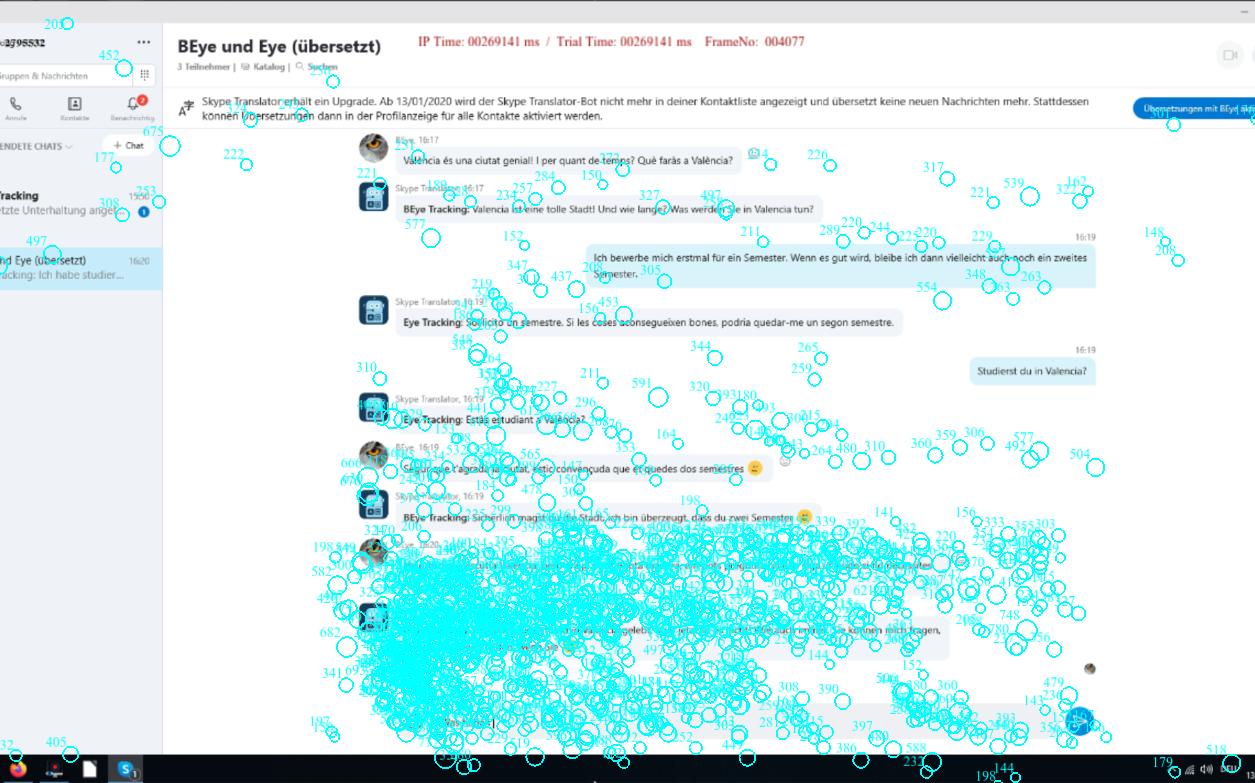
\includegraphics[width=\textwidth]{Figures/Fixmaps/CatDe/Overlay_Image_TN24_Trial_1_Fixations}
	\caption{Fixationen während einer Bildschirmaufnahme\label{K6:fig:fixations-TN24}}
\end{figure}
\vfill\pagebreak


%------------------------------------------------------------------------

%------------------------------------------------------------------------

\begin{figure}
    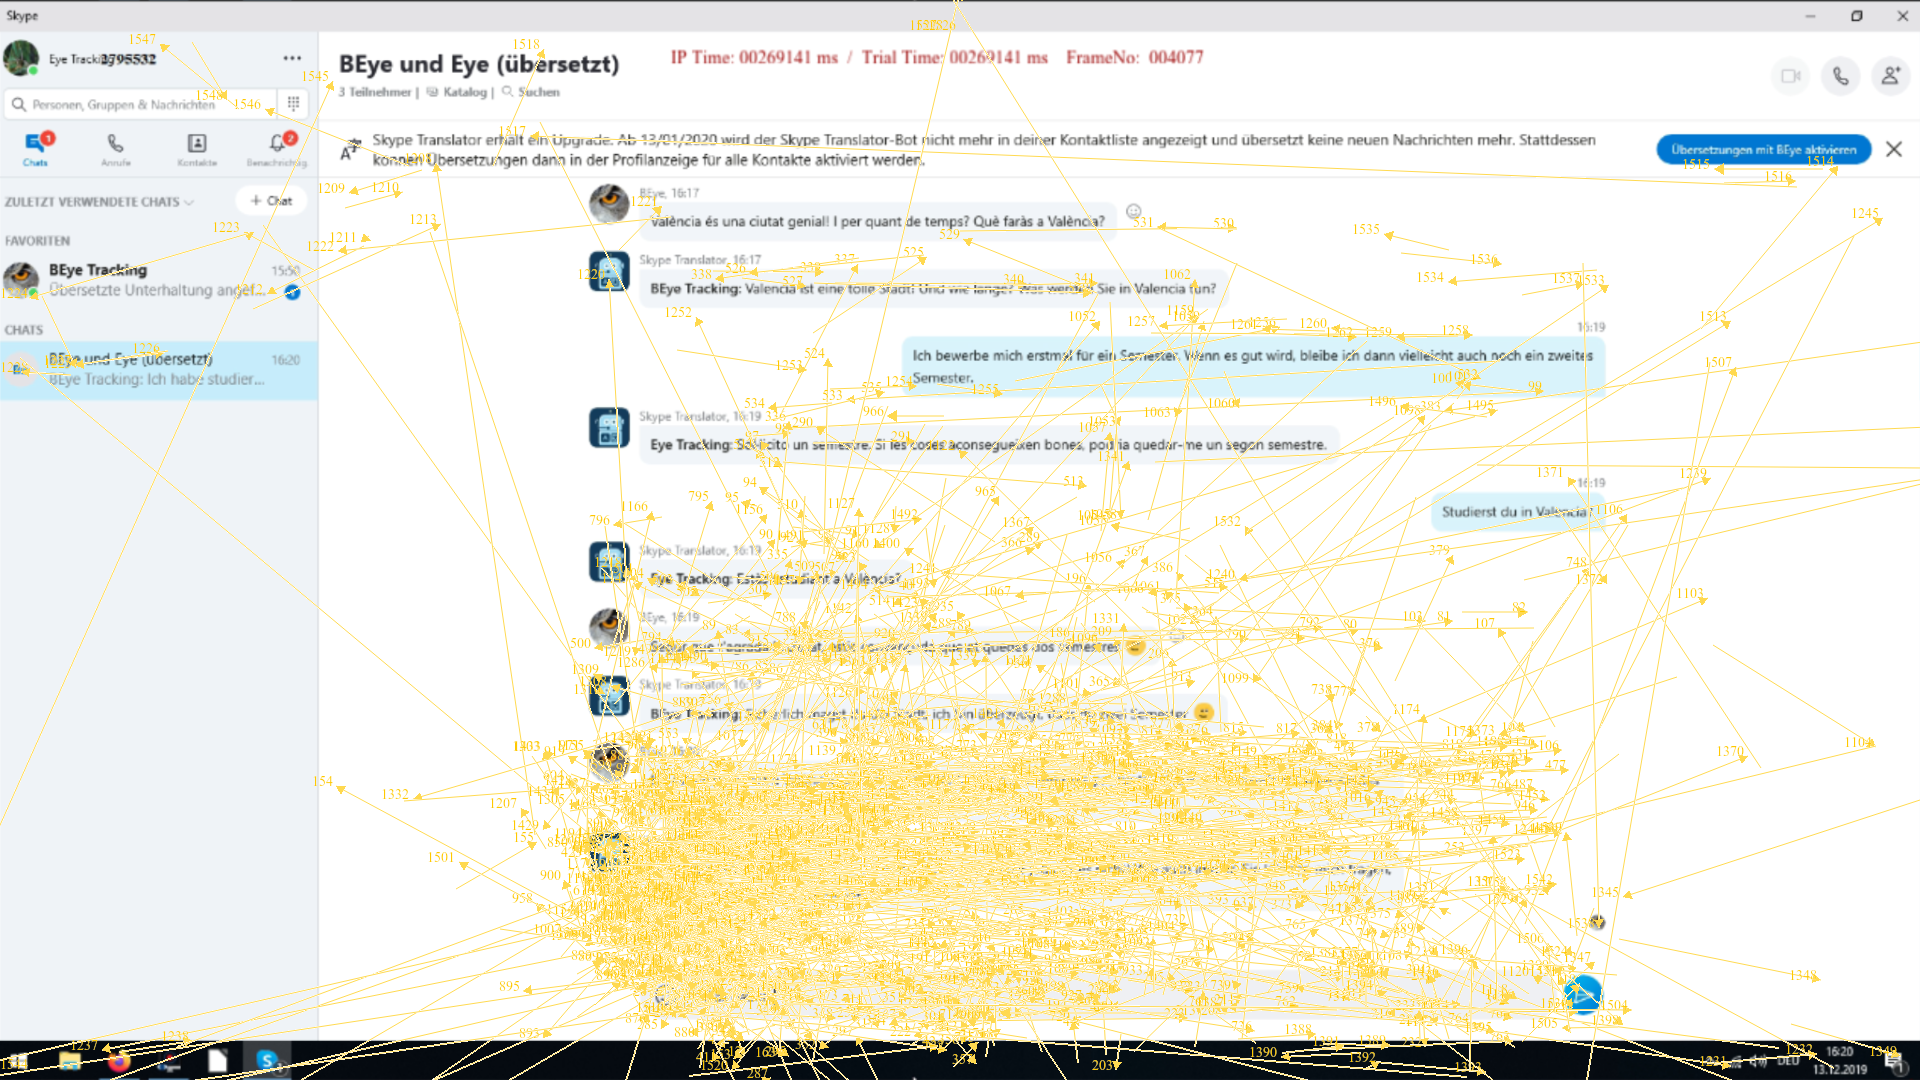
\includegraphics[width=\textwidth]{Figures/Fixmaps/CatDe/Overlay_Image_TN24_Trial_1_Saccades}
	\caption{Sakkaden während einer Bildschirmaufnahme\label{K6:fig:sacmove-TN24}}
\end{figure}


%------------------------------------------------------------------------

Die Sakkaden in der \figref{K6:fig:sacmove-TN24} bilden ebenfalls ein dichtes Netz analog zu dem Muster, das die Fixationen abgeben. Vereinzelt führen Sakkaden über den Bereich hinaus. Das kann verschieden Gründe haben. Die Proband{\textperiodcentered}innen mussten womöglich auf eingehende Nachrichten warten und ließen den Blick über die bestehenden Nachrichten wandern. Ebenso können diese Sakkaden ein vergleichendes Leseverhalten beschreiben, bei dem zu bereits erfassten Informationen zurückgesprungen wurde. Die Nummern an den Spitzen der Feile geben den chronologischen Verlauf der Sakkaden an (den sog. \emph{scan path}\is{Scan Path!Sakkade}) Der wichtigste Bereich ist hier ebenfalls mittig links im unteren Bildschirmbereich oberhalb der Eingabemaske.\largerpage

Die visuelle Aufbereitung der Blinzler während einer Eye-Tracking-Session kann ebenfalls als Indikator für kognitive Auslastung genommen werden. Die roten Linien bilden die Distanz ab, die der Eye-Tracker nicht erfassen konnte, sprich: Der Beginn der Linie ist der Punkt, an dem letztmalig eine Reflektion der Pupille aufgezeichnet wurde und das Ende der Linie der Punkt, an dem darauf folgend wieder eine Reflektion eingefangen wurde. Somit erklären sich auch die roten Linien, die über den Bildschirmrand hinausgehen. Hier ist zu vermuten, dass die Versuchsperson durch einen Reiz im Versuchslabor abgelenkt wurde. Zunächst ist jedoch auch hier festzuhalten, dass sich die erfassten Blinzler\is{Blinzler} oberhalb der Eingabemaske mittig links verdichten. Wie bereits weiter oben erwähnt, werden an dieser Stelle die MÜ-Ausgabe sowie die eingehenden Nachrichten des Gegenübers angezeigt.

%------------------------------------------------------------------------

\begin{figure}
    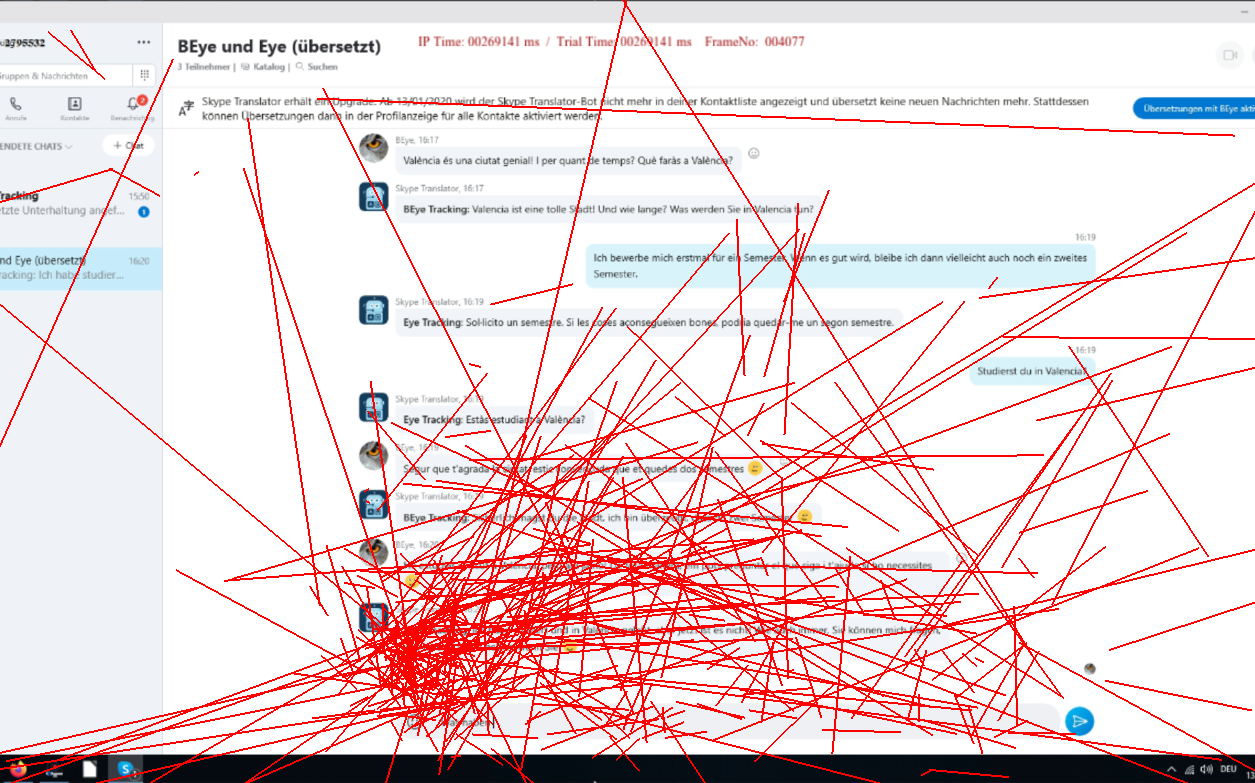
\includegraphics[width=\textwidth]{Figures/Fixmaps/CatDe/Overlay_Image_TN24_Trial_1_Blinks}
	\caption{Blinzler während einer Bildschirmaufnahme\label{K6:fig:blinks-TN24}}
\end{figure}


%------------------------------------------------------------------------


%------------------------------------------------------------------------

\subsection{Fixationen der Probanden}

\label{K6:sub:Fixationen:CatDe}

%------------------------------------------------------------------------


%------------------------------------------------------------------------

\subsubsection{Fixationsanzahl}
\label{K6:subsubsec:fixcount:CatDe}

%------------------------------------------------------------------------

\is{Fixation!-sanzahl|(}
\tabref{K6:tab:CatDe:mean-sd-fixc} zeigt die aufsummierte Anzahl an Fixationen pro AOI-Kategorie\is{Area of Interest!Kategorie}. Insgesamt wurden 21.196 Fixationen in den mit AOI versehenen Bereichen erfasst. Der Gesamtschnitt beträgt 12,96 Fixationen pro AOI. Die maschinelle Übersetzung\is{maschinelle Übersetzung} ins Deutsche (\emph{GerMT}) erhielt mit 7.037 Fixationen etwa zweieinhalb Mal so viele wie die deutschsprachigen Originale (2.469). Auch die maschinelle Übersetzung ins Katalanische erhielt mehr Fixationen (4.553) als die katalanischsprachigen Originale (3.046). Das Eingabefeld wurde 4.097 Mal fixiert. Der Durchschnittswert für die katalanischen Originalbeiträge ist mit 6,99 am kleinsten. Auch die durchschnittliche Fixationsanzahl auf die deutschen Originalbeiträge liegt mit 8,20 unter dem Gesamtschnitt. Nur die mittlere Anzahl an Fixationen, die auf die MÜ\is{maschinelle Übersetzung} ins Deutsche und auf die Eingabemaske verfallen, liegen über dem Schnitt (jeweils 13,8 und 195,1).

%------------------------------------


	
\begin{table}

\begin{tabular}{lrS[table-format=3.2]rr}  
\lsptoprule
    {AOI-Kategorie} & \multicolumn{1}{c}{Summe} & {Mittelwert} & \multicolumn{1}{c}{Median} & \multicolumn{1}{c}{SD} \\
\midrule
    GerO   & 2.469 & 8,20 & 4 & 15,05 \\ 
    CatMT   & 4.552 & 12,34 & 7 &  17,85\\ 
    CatO 	& 3.041 & 6,99 & 3 & 10,97\\ 
    GerMT	& 7.037 & 13,8 & 9 & 16,45\\ 
    Eingabe   & 4.097 & 195,1 & 188 & 102,29 \\ 
    \midrule
    Global  & 21.196 & 12,96 & 6 & 28,24\\ 
\lspbottomrule
\end{tabular}
    \caption[Summe, Mittelwert, Median und SD der Fixationsanzahl]{Summe, Mittelwert, Median und SD der Fixationsanzahl pro AOI-Kategorie}
\label{K6:tab:CatDe:mean-sd-fixc}
\end{table}
	

%------------------------------------


% %------------------------------------------------------------------------

% \begin{figure}[htbp]
% 	%\centering
% 		\centerline{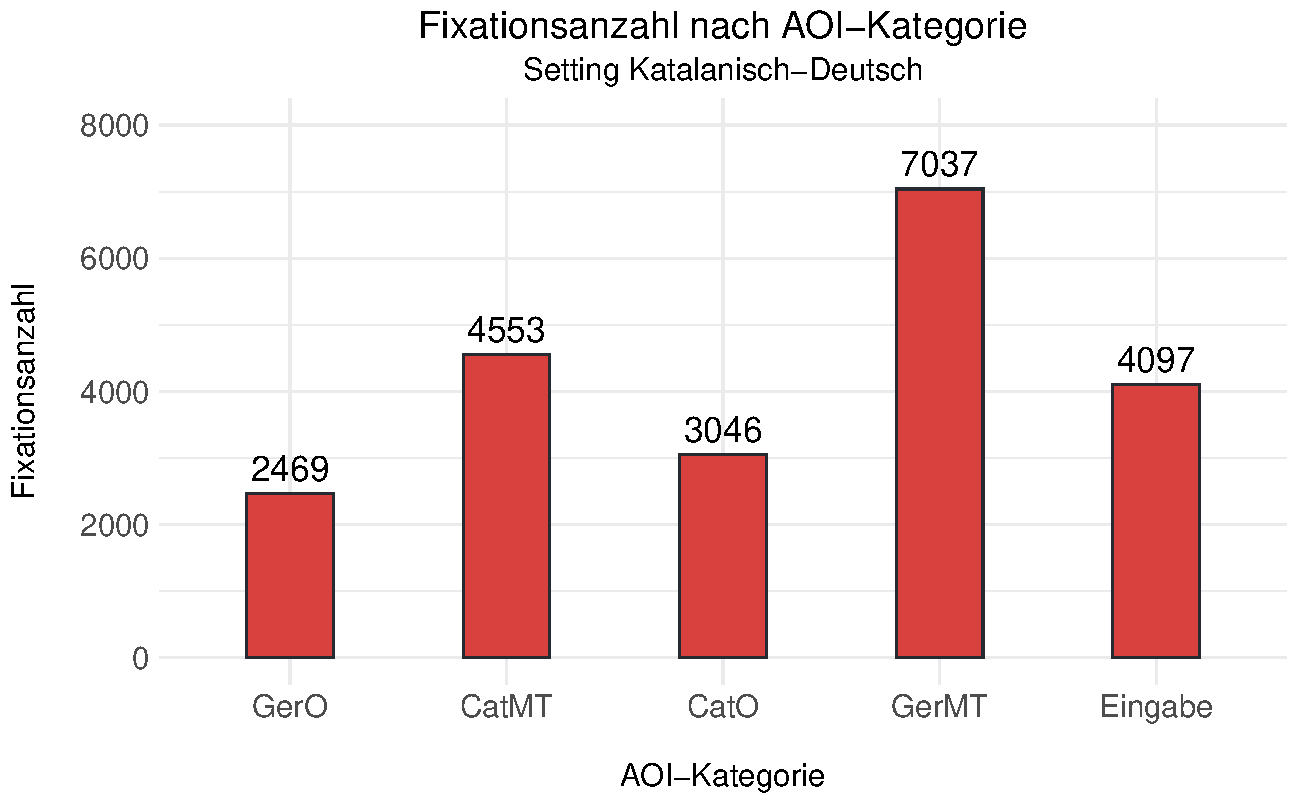
\includegraphics[width=\textwidth]{Figures/EyeTracking/CatDe/ggplot_catde_ffcount_AOI_de}}
% 	\caption{Aufsummierte Fixationsanzahlen nach AOI im Setting Katalanisch-Deutsch}
%     \label{K6:fig:FixCount-CatDe-AOI}
% \end{figure}

% %------------------------------------------------------------------------

Sowohl die visuelle Inspektion als auch die statistische Untersuchung deuten darauf hin, dass die Fixationsanzahl nicht normalverteilt ist. Ein Shapiro-Wilk-Test ergibt für den gesamten Datensatz ($W = 0,36, p < 0,001$). Eine logarithmische Transformation ändert an dieser Beobachtung nichts (Shapiro-Wilk Test, log10: $W = 0,97, p < 0,001$). Deshalb wird die Fixationsanzahl mit nicht-parametrischen Tests analysiert. 

\begin{sloppypar}
Ein Kruskal-Wallis-Test\is{Kruskal-Wallis-Test|see{Statistik}}\is{Statistik!Testverfahren!Kruskal-Wallis-Test} zeigt, dass die Fixationsanzahl pro AOI nach den einzelnen Teilnehmer{\textperiodcentered}innen variiert ($\chi^2(20) = 252,11, p < 0,01$). Anschließend durchgeführte Post-hoc-Tests (Dunn-Benjamini-Hochberg-Tests)\is{Dunn-Benjamini-Hochberg-Test|see{Statistik}}\is{Statistik!Testverfahren!Dunn-Benjamini-Hochberg-Test} zeigen, dass sich 132 von 210 TN-Gruppen (62,86\,\%) signifikant unterscheiden. Ein zweiter Kruskal-Wallis-Test\is{Statistik!Testverfahren!Kruskal-Wallis-Test} zeigt, dass die Fixationsanzahl von der betrachteten AOI-Kategorie beeinflusst wird ($\chi^2(4) = 245,9, p < 0,01$). Anschließend durchgeführte Post-hoc-Tests (Dunn-Benjamini-Hochberg-Tests,  s. \tabref{K6:tab:CatDe:dunntest-fixcount}\is{Statistik!Testverfahren!Dunn-Benjamini-Hochberg-Test}) zeigen, dass sich alle bis auf eine Gruppierung (CatO-GerO) voneinander unterscheiden, sodass gefolgert werden kann, dass sich die zentrale Tendenz aller AOI-Kategorien mit Ausnahme der Gruppierung \emph{CatO-GerO} signifikant unterscheiden. Es handelt sich um schwache bis mittlere Effekte\is{Effektstärke nach Cohen}\is{Statistik!Testverfahren!Effektstärke nach Cohen} nach \citet{cohen_power_1992} mit $0,1 < r < 0,5$.
\end{sloppypar}

%------------------------------------


	
\begin{table}

\begin{tabular}{lS[table-format=-2.6]S[table-format=1.4]@{ }lS[table-format=1.2]}  
\lsptoprule
        {AOI-Kategoriepaar} & {$z$} & \multicolumn{2}{c}{$p$ (angepasst)} & {Effekt}\\ 
\midrule
        CatMT-CatO    &  8,105397 & 0,0000 & ***  & 0,29\\ 
        CatMT-Eingabe & -6,479862 & 0,0000 & ***  & 0,33 \\ 
        CatO-Eingabe  & -9,074030 & 0,0000 & ***  & 0,42 \\ 
        CatMT-GerMT   & -3,327846 & 0,0005 & **   & 0,11 \\ 
        CatO-GerMT    & -12,27414 & 0,0000 & ***  & 0,4 \\ 
        Eingabe-GerMT &  5,507214 & 0,0000 & ***  & 0,24 \\ 
        CatMT-GerO    &  6,185499 & 0,0000 & ***  & 0,21 \\ 
        CatO-GerO     & -1,243531 & 0,1068 &      &  \\ 
        Eingabe-GerO  &  8,569340 & 0,0000 & ***  & 0,37 \\ 
        GerMT-GerO    &  9,738661 & 0,0000 & ***  & 0,34 \\ 
    \lspbottomrule
        
    \end{tabular}
        \caption{Ergebnisse des Dunn-Tests: Gruppierte Vergleiche der Fixationsanzahl nach AOI-Kategorie}
    \label{K6:tab:CatDe:dunntest-fixcount}
\end{table}


%------------------------------------

Weiterhin ergibt ein durchgeführter Mann-Whitney-U-Test\is{Mann-Whitney-U-Test|see{Statistik}}\is{Statistik!Testverfahren!Mann-Whitney-U-Test}, dass sich die zentrale Tendenz der Fixationsanzahl pro AOI-Kategorie unter Beteiligung der progressiven ersten Fixation\is{Fixation!progressive erste} signifikant unterscheidet. Im Falle des gesamten Datensatzes ($U = 360.541,00, p < 0,001$) wurden mehr Fixationen getätigt, wenn die AOI in konsekutiver Reihenfolge betreten wurden (Median: 7) als wenn zunächst ein AOI mit höherer Ordnungszahl betrachtet wurde (Median: 4). Nach AOI-Kategorie unterteilt betrachtet ergeben sich folgende Werte: Der Mann-Whitney-U-Test für das deutsche Original ($U = 21.050,00, p < 0,01$) deutet ebenfalls darauf hin, dass signifikante Unterschiede in der zentralen Tendenz der Fixationsanzahl unter Beachtung der progressiven ersten Fixation\is{Fixation!progressive erste} vorliegen. In konsekutiver Reihenfolge beträgt der Median der Fixationsanzahl 5, nach Betrachtung eines AOI mit höherer Ordnungszahl 3. Auch bei der Untersuchung der MÜ ins Katalanische weist der Mann-Whitney-U-Test\is{Statistik!Testverfahren!Mann-Whitney-U-Test} signifikante Werte ($U = 11.844,00,\allowbreak\ p < 0,05$) auf. Hier beträgt der Median für Fixationen in konsektutiver Abfolge 7, nach Betrachtung von AOI höheren Ranges 5. Im Falle des katalanischen Orignals ergibt der Test ebenso signifikante Unterschiede ($U = 44.397,50, p < 0,001$), wobei der Median für die Fixationsanzahl in chronologischer 4 und in ungeordneter Reihenfolge 3 beträgt. Die abschließende Betrachtung der MÜ ins Deutsche weist auch signifikante Werte auf ($U = 21.282,00, p < 0,01$). Der Median der Fixationsanzahl bei konsekutiver Abfolge beträgt 10, bei ungeordneter Reihenfolge 7.

Zur genaueren Einordnung sind in \tabref{K6:tab:CatDe:mean-sd-iaarea} (S.\,\pageref{K6:tab:CatDe:mean-sd-iaarea}) Summe, Mittelwert und Standardabweichung der AOI-Größe in Pixeln pro AOI-Kategorie aufgeführt. Die Analyse der AOI-Größe ist jedoch aufgrund der in Abschnitt~\ref{K5:subsubsec:DynAOI} (S.\,\pageref{K5:subsubsec:DynAOI}) beschriebenen technischen Ungenauigkeit der Annotation nur eine Annäherung. Dabei zeigt ein Korrelationstest nach Spearman\is{Spearman's Rho}\is{Korrelationstest nach Spearman}\is{Statistik!Testverfahren!Korrelationstest nach Spearman}, dass die Anzahl an Fixationen pro AOI-Kategorie positiv und signifikant mit der Größe des AOI\is{Area of Interest!Größe des} zusammenhängt ($r_{s} = 0,52, p < 0,01, n = 349.055.310$). Das Bestimmtheitsmaß beträgt 27,22\,\%. Der Test geht dabei von einer nicht normalen Verteilung der Daten aus. Spearman's Rho\is{Spearman's Rho}\is{Korrelationstest nach Spearman}\is{Statistik!Testverfahren!Korrelationstest nach Spearman} nimmt Werte zwischen -1 und 1 ein: -1 deutet auf eine stark negative Korrelation hin, 0 zeigt keinerlei Beziehung zwischen den Variablen an und 1 verweist auf eine stark positive Korrelation\footnote{S. hierzu \href{http://www.sthda.com/english/wiki/correlation-test-between-two-variables-in-r}{http://www.sthda.com/english/wiki/correlation-test-between-two-variables-in-r}, letzter Aufruf am \datum{}.}.


%------------------------------------


\begin{table}
\begin{tabular}{lrrr}  
\lsptoprule
    \multicolumn{1}{c}{AOI-Kategorie} & \multicolumn{1}{c}{Summe} & \multicolumn{1}{c}{Mittelwert} & \multicolumn{1}{c}{SD} \\ 
    \midrule
    GerO  & 8.437.392 & 28.031,20 & 19.022,38 \\ 
    CatMT & 10.410.362 & 28.212,36 & 16.537,87 \\ 
    CatO & 10.702.559 & 24.603,58 & 18.337,66 \\ 
    GerMT & 15.975.212 & 31.323,95 & 17.908,85 \\ 
    Eingabe & 1.462.981 & 69.665,76  & 5.164,34 \\ 
    \midrule
    Gesamt & 46.988.507 & 28.721,58 & 18.592,74 \\ 
    \lspbottomrule
\end{tabular}
    \caption{Summe, Mittelwert und SD der AOI-Größe in px pro AOI-Kategorie\label{K6:tab:CatDe:mean-sd-iaarea}}
\end{table}

%------------------------------------

\is{Fixation!-sanzahl|)}
   

%------------------------------------------------------------------------

\subsubsection{Dauer der ersten Fixation}
\label{K6:subsubsec:iaffd:catde}

%------------------------------------------------------------------------

\is{Fixation!Dauer der ersten|(}
Wie in \tabref{K6:tab:CatDe:mean-sd-iaffd} und \figref{K6:fig:CatDe:firstfix-mean-box} ersichtlich wird, liegt die durchschnittliche Dauer der ersten Fixation auf den eingehenden Nachrichten 15\,ms unter dem Gesamtschnitt, wohingegen die Fixationsdauer\is{Fixation!-sdauer} auf den eigenen Nachrichten 7\,ms überhalb des Schnittes liegt. Der Wert bei Betrachtung der Eingabemaske liegt lediglich 2\,ms vom Durchschnitt entfernt. Mit durchschnittlich 304\,ms ist die Dauer der ersten Fixation auf den katalanischen Originalen auffällig lange.

\begin{table}
\begin{tabular}{lrrr}  
\lsptoprule
    \multicolumn{1}{c}{AOI-Kategorie} & \multicolumn{1}{c}{Mittelwert} & \multicolumn{1}{c}{Median}  & \multicolumn{1}{c}{SD} \\ 
    \midrule
    GerO   & 298,98 & 245,0 & 157,89 \\ 
    CatMT   & 288,61 & 234,5 & 162,41\\ 
    CatO 	& 304,13 & 257,0 & 152,42\\ 
    GerMT	& 277,94 & 234,0 & 141,96\\ 
    Eingabe   & 290,26 & 228,0 & 174,23 \\ 
    \midrule
    Global  & 292,01 & 242,0 & 153,23\\ 
    \lspbottomrule
\end{tabular}
    \caption[Mittelwert, Median und SD der Dauer der ersten Fixation]{Mittelwert, Median und SD der Dauer der ersten Fixation pro AOI-Kategorie}
\label{K6:tab:CatDe:mean-sd-iaffd}
\end{table}


%------------------------------------------------------------------------

\begin{figure}[p]
    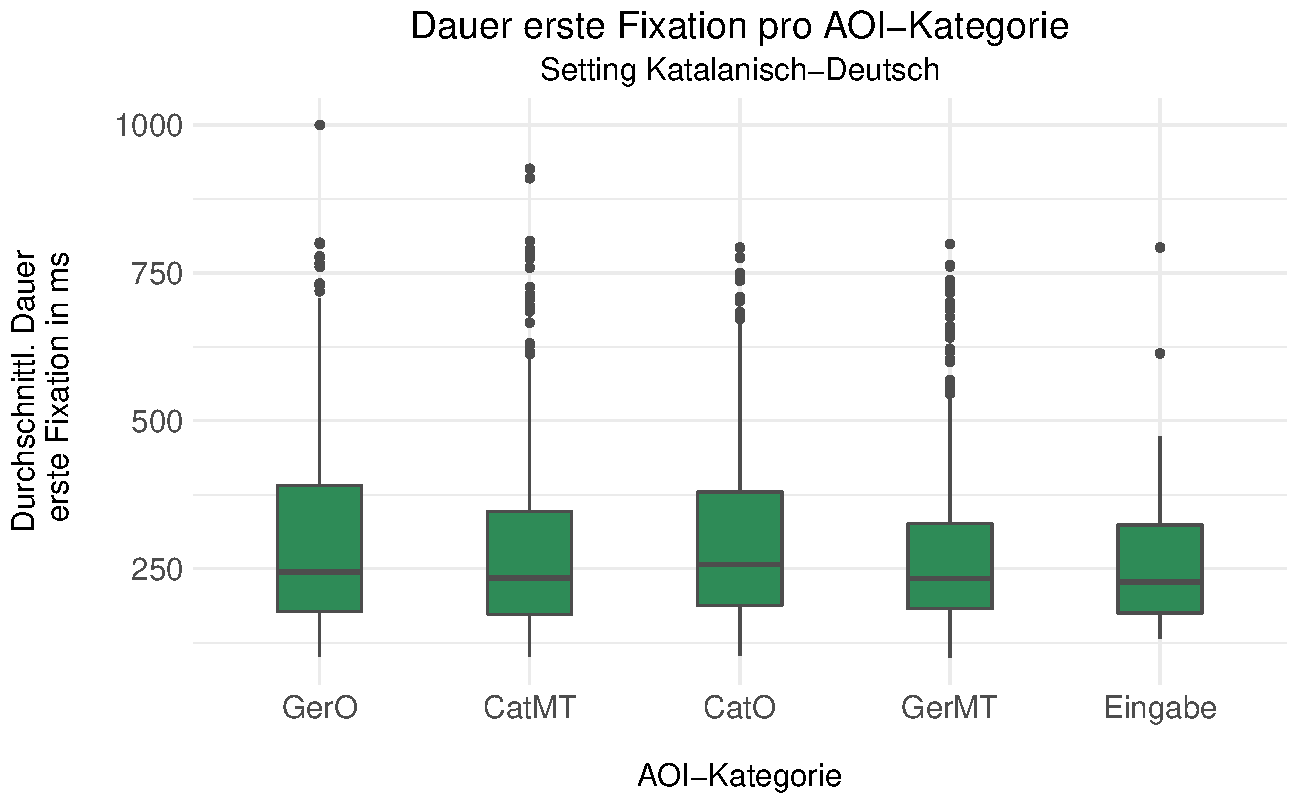
\includegraphics[width=\textwidth]{Figures/EyeTracking/CatDe/ggplot_catde_boxplot_meanffdur_AOI_de.pdf}
	\caption{Durchschnittliche Fixationsdauer pro AOI}
    \label{K6:fig:CatDe:firstfix-mean-box}
\end{figure}

\begin{figure}[p]
    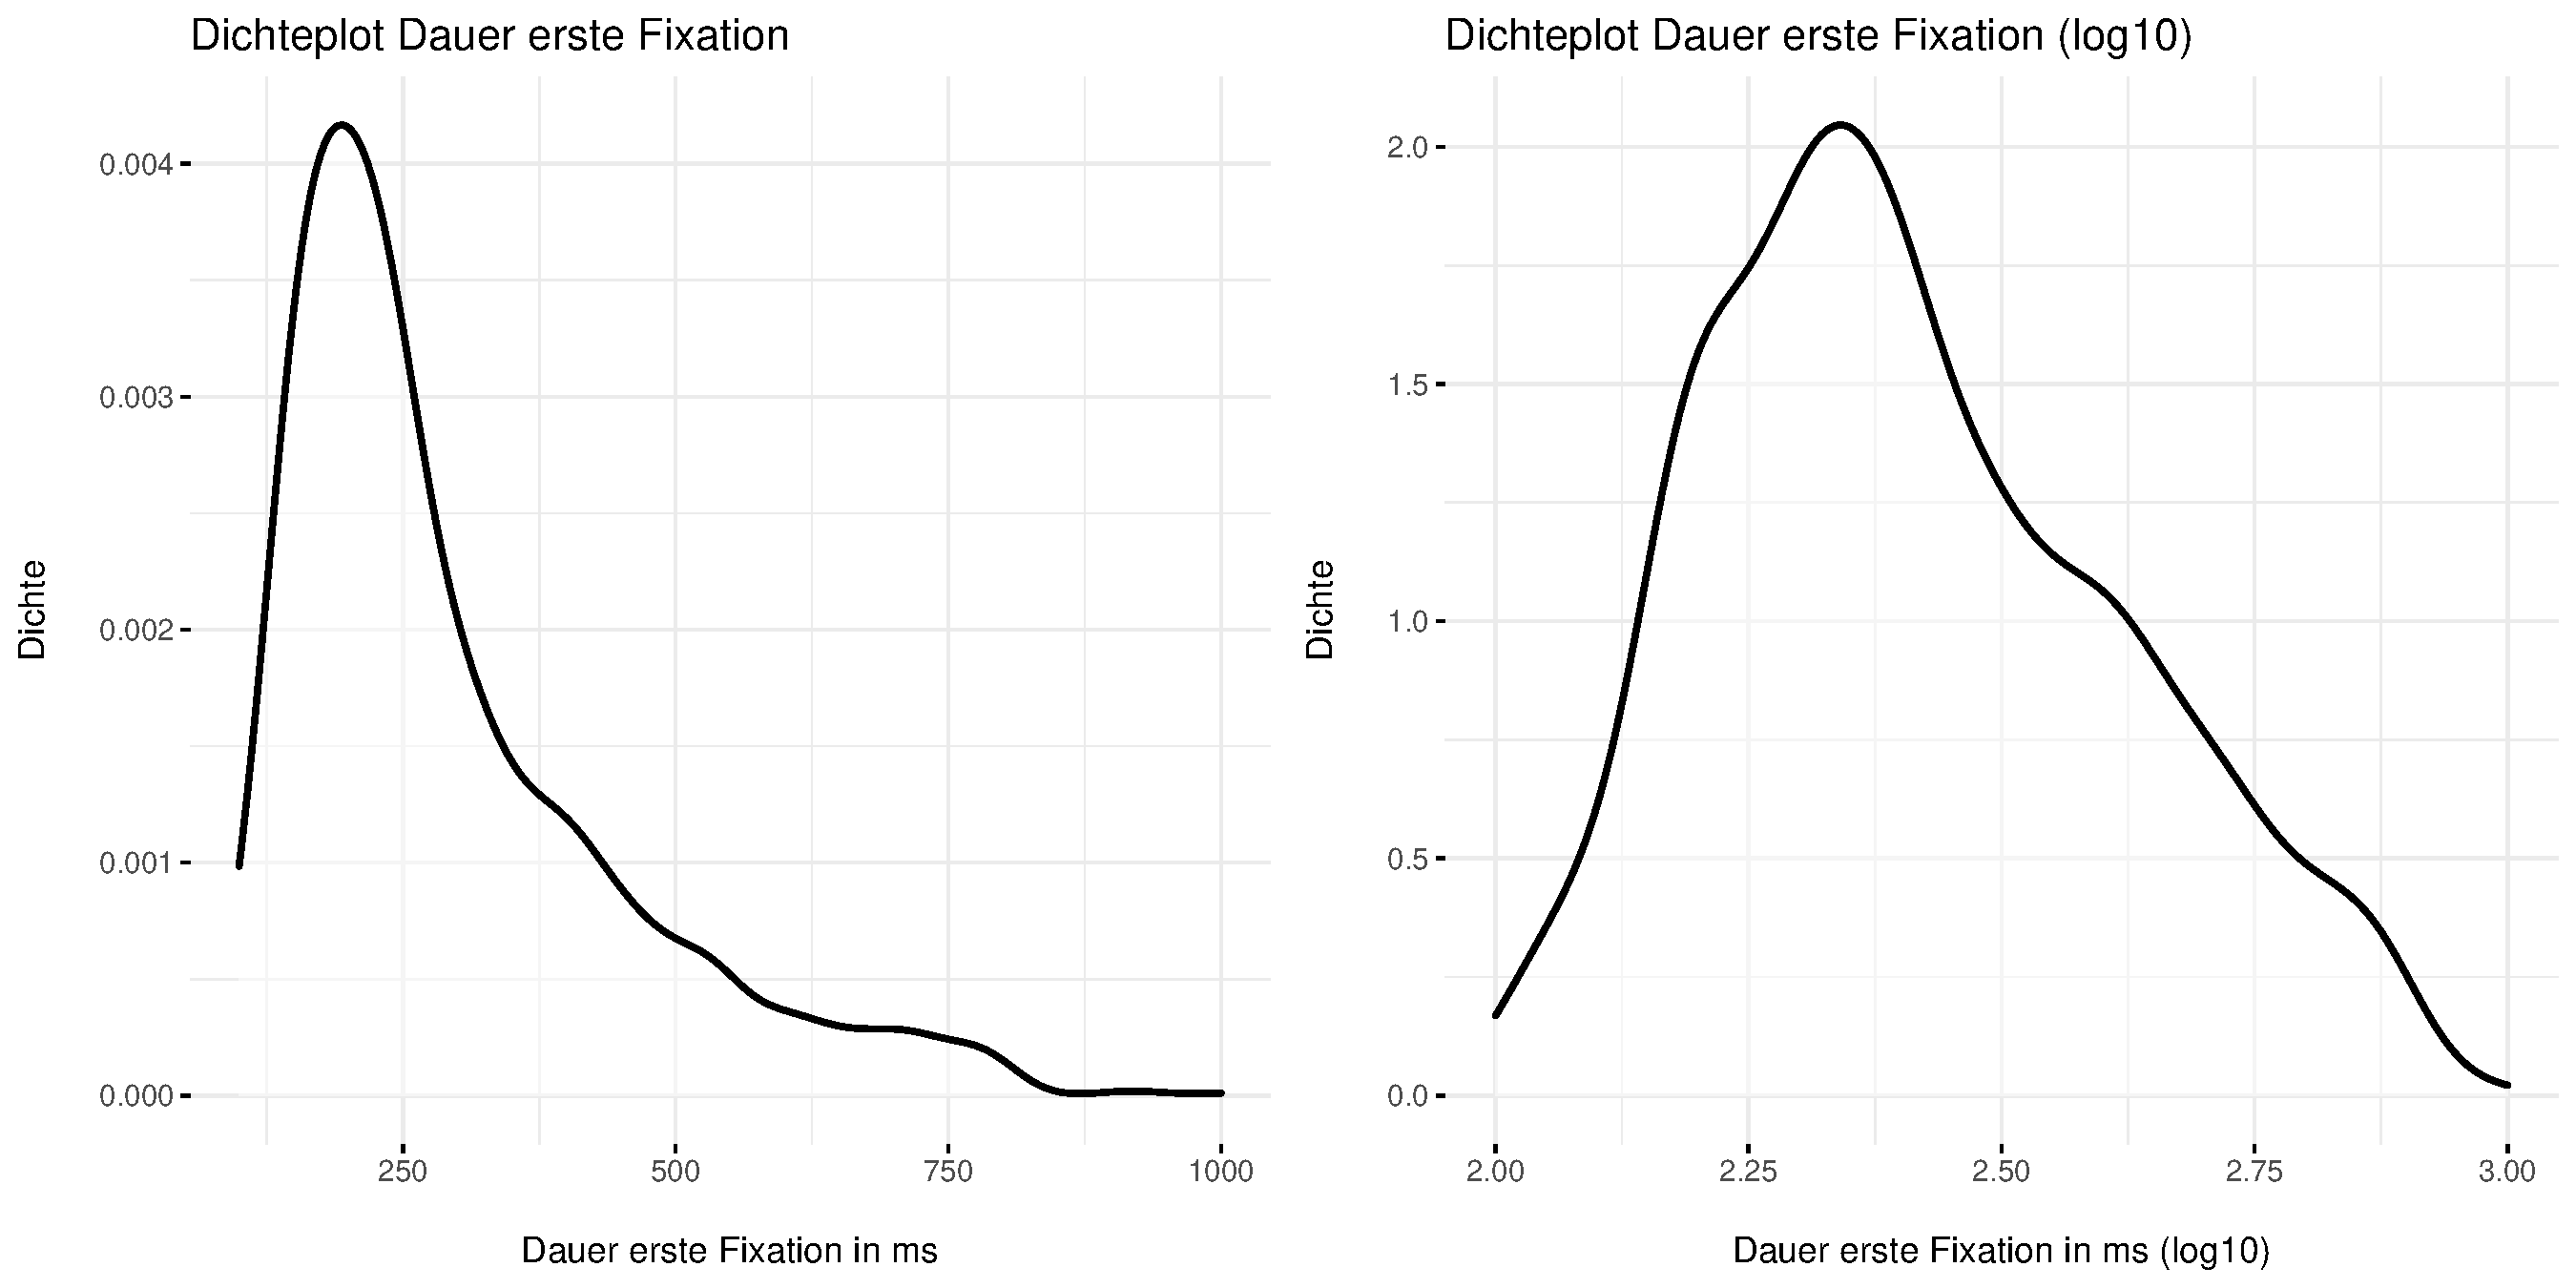
\includegraphics[width=\textwidth]{Figures/EyeTracking/CatDe/ggplot_CatDe-FFDur_density_de}
	\caption{Verteilung der Dauer der ersten Fixation: normal (links), logarithmisch transformiert (rechts)}
	\label{K6:fig:CatDe:density-ffdur}
\end{figure}


%------------------------------------------------------------------------

Sowohl die graphische als auch statistische Inspektion\is{Inspektion!graphische}\is{Inspektion!statistische} der Daten deutet darauf hin, dass keine Normalverteilung vorliegt. Eine logarithmische Transformation nähert die Verteilung zwar der Gausschen Glockenkurve an, ist jedoch noch immer leicht verschoben (s. \figref{K6:fig:CatDe:density-ffdur}). Auch eine Berechnung der Schiefe (normal: 1,67, log-trans\-for\-miert: 0,46) und der Kurtosis\is{Kurtosis} (normal: 3,30, log-trans\-for\-miert: $-0,25$) sowie der Shapiro-Wilk-Test (normal: $W = 0,86, p < 0,001$, log-trans\-for\-miert: $W = 0,96, p < 0,001$) deuten darauf hin, dass der Datensatz nicht normalverteilt ist. Deshalb werden für die statistische Analyse dieser Daten nicht-parametrische Tests\is{Statistik!Testverfahren!nicht-parametrisches} verwendet.

\begin{sloppypar}
Ein Kruskal-Wallis-Test\is{Statistik!Testverfahren!Kruskal-Wallis-Test} zeigt, dass Unterschiede in der zentralen Tendenz der Fixationsdauer zwischen den einzelnen Teilnehmer{\textperiodcentered}innen bestehen ($\chi^2(6) = 76,06,\allowbreak\ p < 0,01$). Anschließend durchgeführte Post-hoc-Tests (Dunn-Ben\-ja\-mi\-ni-Hoch\-berg-Tests)\is{Statistik!Testverfahren!Dunn-Benjamini-Hochberg-Test} zeigen, dass sich 67 von 210 TN-Gruppen (31,9\,\%) signifikant unterscheiden. Es kann gefolgert werden, dass die Fixationsdauer in gewissem Maße durch die Teilnehmer{\textperiodcentered}innen beeinflusst wird.
\end{sloppypar}

Ein weiterer Kruskal-Wallis-Test\is{Statistik!Testverfahren!Kruskal-Wallis-Test} in Kombination mit anschließend durchgeführten Post-hoc-Tests (Dunn-Benjamini-Hochberg-Tests\is{Statistik!Testverfahren!Dunn-Benjamini-Hochberg-Test}, s. \tabref{K6:tab:CatDe:dunntest-ffdur}) zeigt, dass keine signifikanten Unterschiede in der zentralen Tendenz der Dauer der ersten Fixation zwischen den einzelnen AOI-Kategorien bestehen ($\chi^2(4) = 8,73,\allowbreak\ p = 0,07$). Auch bei testweisem Ausschluss der Kategorie \glqq Eingabe\grqq{} verändern sich die Werte kaum. Hierbei ist jedoch zu beachten, dass -- wie bereits im empirischen Teil problematisiert -- die Schrift- bzw. Fenstergröße der einzelnen AOI zu gering ist, als dass der Eye-Tracker die Fixationen pro Wort hätte präzise festhalten können. Dem entgegenzuhalten ist jedoch, dass die dynamischen AOI ohnehin nicht auf Wortebene konzipiert sind, sodass die Dauer der ersten Fixation pro AOI weniger für die anfängliche Verarbeitung eines Wortes steht, sondern vielmehr auf den ganzen Textbaustein zu beziehen ist.

%------------------------------------

\vfill
\begin{table}[H]
\begin{tabular}{lS[table-format=-1.6]S[table-format=1.4]c}  
\lsptoprule
    {AOI-Kategoriepaar} & {$z$} & {$p$ (angepasst)} & {Effekt}\\ 
    \midrule
    CatMT-CatO    & -2,327723 & 0,0498 & - \\ 
    CatMT-Eingabe &  0,080594 & 0,5849 & -  \\ 
    CatO-Eingabe  &  0,812292 & 0,3472 & -  \\ 
    CatMT-GerMT   &  0,049745 & 0,4802 & -  \\ 
    CatO-GerMT    &  2,561243 & 0,0521 & -  \\ 
    Eingabe-GerMT & -0,065733 & 0,5264 & -  \\ 
    CatMT-GerO    & -1,274422 & 0,2531 & -  \\ 
    CatO-GerO     &  0,880663 & 0,3785 & -  \\ 
    Eingabe-GerO  & -0,516368 & 0,4326 & -  \\ 
    GerMT-GerO    & -1,401717 & 0,2683 & -  \\ 
    \lspbottomrule
\end{tabular}
    \caption{Ergebnisse des Dunn-Tests: Gruppierte Vergleiche der Dauer der ersten Fixation nach AOI-Kategorie\label{K6:tab:CatDe:dunntest-ffdur}}
\end{table}
\vfill\pagebreak


%------------------------------------

Weiterhin sollen die Unterschiede zwischen der Fixationsdauer und der progressiven ersten Fixation untersucht werden, die allerdings nur in zwei Ausprägungen vorliegt (0 und 1). Es wird daher nicht der Kruskal-Wallis-Test, sondern der Mann-Whitney-U-Test\is{Statistik!Testverfahren!Mann-Whitney-U-Test} verwendet. Es besteht ein signifikanter Unterschied in der zentralen Tendenz der Dauer zwischen den AOI, bei denen zuvor ein AOI mit höherer Ordnungszahl betrachtet wurde, und denen, die chronologisch betreten wurden. Die eigenen Chatbeiträge der Versuchspersonen werden kürzer fixiert, wenn zuvor ein AOI mit höherer Ordnungszahl betrachtet wurde, als wenn es sich um eine tatsächliche chronologische erstmalige Fixation handelt (Rangmediane 808,64 zu 706,78). Ein exakter Mann-Whitney-U-Test\is{Statistik!Testverfahren!Mann-Whitney-U-Test} ($U = 426.963,00, p < 0,01, r = 0,11$) in Verbindung mit einer Untersuchung der Effektstärke\is{Effektstärke nach Cohen}\is{Statistik!Testverfahren!Effektstärke nach Cohen} nach \citet{cohen_power_1992} zeigt dabei allerdings nur einen schwachen Effekt.

Betrachtet man die Art der ersten Fixation nach AOI-Kategorie getrennt, so weist lediglich die zentrale Tendenz der progressiven ersten Fixation bei Betrachtung der maschinellen Übersetzung ins Deutsche (\emph{GerMT}) einen signifikanten Unterschied auf ($U = 22.014,00, r < 0,01, r = 0,16$, s. \tabref{K6:tab:CatDe:mwutest-ffdur-ffixpro}). Auch hier ist die Effektstärke\is{Effektstärke nach Cohen}\is{Statistik!Testverfahren!Effektstärke nach Cohen} nach \citet{cohen_power_1992} nur schwach. Erfolgt die Fixation, nachdem ein AOI mit höherer Ordnungszahl betreten wurde, so dauert sie länger als wenn die Fixation chronologisch erfolgte (Rangmediane 212,03 zu 265,23).

%------------------------------------



\begin{table}
\begin{tabular}{lrS[table-format=1.3]@{ }lcS[table-format=1.2]}  
\lsptoprule
    {AOI-Kategorie} & \multicolumn{1}{c}{$U$} & \multicolumn{2}{c}{$p$ (angepasst)} & {Effekt}\\\midrule
    GerO & 21.981,0 & 0,26  & \\ 
    CatMT  & 12.603,0 & 0,25  & \\ 
    CatO  & 47.480,5 & 0,07  & \\ 
    GerMT  & 22.014,0 & 0,001 & *** & 0,16 \\ 
    Eingabe & \multicolumn{1}{c}{n/a} & n/a \\\midrule
    Global & 426.963,0 & 0,001 & *** & 0,11 \\ 
    \lspbottomrule
\end{tabular}
    \caption{Ergebnisse des Mann-Whitney-$U$-Tests: Vergleiche der Dauer der ersten Fixation nach AOI-Kategorie und progressiver ersten Fixation\label{K6:tab:CatDe:mwutest-ffdur-ffixpro}}
\end{table}


%------------------------------------

Ein durchgeführter Korrelationstests (Spearman’s Rho)\is{Spearman's Rho}\is{Spearman's Rho|see{Statistik}}\is{Korrelationstest nach Spearman}\is{Statistik!Testverfahren!Korrelationstest nach Spearman} belegt, dass signifikante Zusammenhänge zwischen Fixationsdauer und der Größe der AOI\is{Area of Interest!Größe des} bestehen ($r_{s} = -0,14, p < 0,01, n = \num{6,31e08}$). Dabei handelt es sich nach \citet{cohen_power_1992} um einen schwachen Effekt. Das Bestimmtheitsmaß beträgt 38.02\,\%.
\is{Fixation!Dauer der ersten|)}

%------------------------------------------------------------------------

\subsubsection{Regressionen}
\label{K6:Subsubsec:regression:catde}

%------------------------------------------------------------------------

\is{Regression!eingehende|(}
%------------------------------------------------------------------------

\subsubsubsection{Eingehende Regressionen}
\label{K6:para:regin:catde}


\figref{K6:fig:CatDe:RegIn-AOI-Count} und \tabref{K6:tab:CatDe:mean-sd-regin} (S.\,\pageref{K6:tab:CatDe:mean-sd-regin}) zeigen die aufsummierte Anzahl aller Regressionen\is{Regression!Summe aller} in ein AOI nach Kategorie sowie deren Mittelwert und Standardabweichung. Auf das katalanische Original und die Eingabemaske verfielen dabei die meisten Regressionen (\emph{CatO}: 504, \diameter\,1,16, SD: 1,52, \emph{Eingabe}: 548, \diameter\,26,1, SD: 14,6), die wenigsten Regressionen wurden in AOI der MÜ ins Katalanische gemacht (\emph{CatMT}: 249, \diameter\,0,67, SD: 1,09). Das deutsche Original und die maschinelle Übersetzung ins Deutsche erhielten jeweils 312 (\diameter\,1,04, SD: 2,39) bzw. 332 (\diameter\,0,65, SD: 1,07) Regressionen. Im Schnitt wird jeweils auf das deutsche und das katalanische Original also somit mindestens ein Rücksprung ausgeführt. Die Eingabemaske weist einerseits viele eingehende Regressionen in absoluten Zahlen auf, andererseits sind auch der Mittelwert mit 26,1 und die Standardabweichung mit 14,6 auffällig hoch.

\begin{figure}[p]
    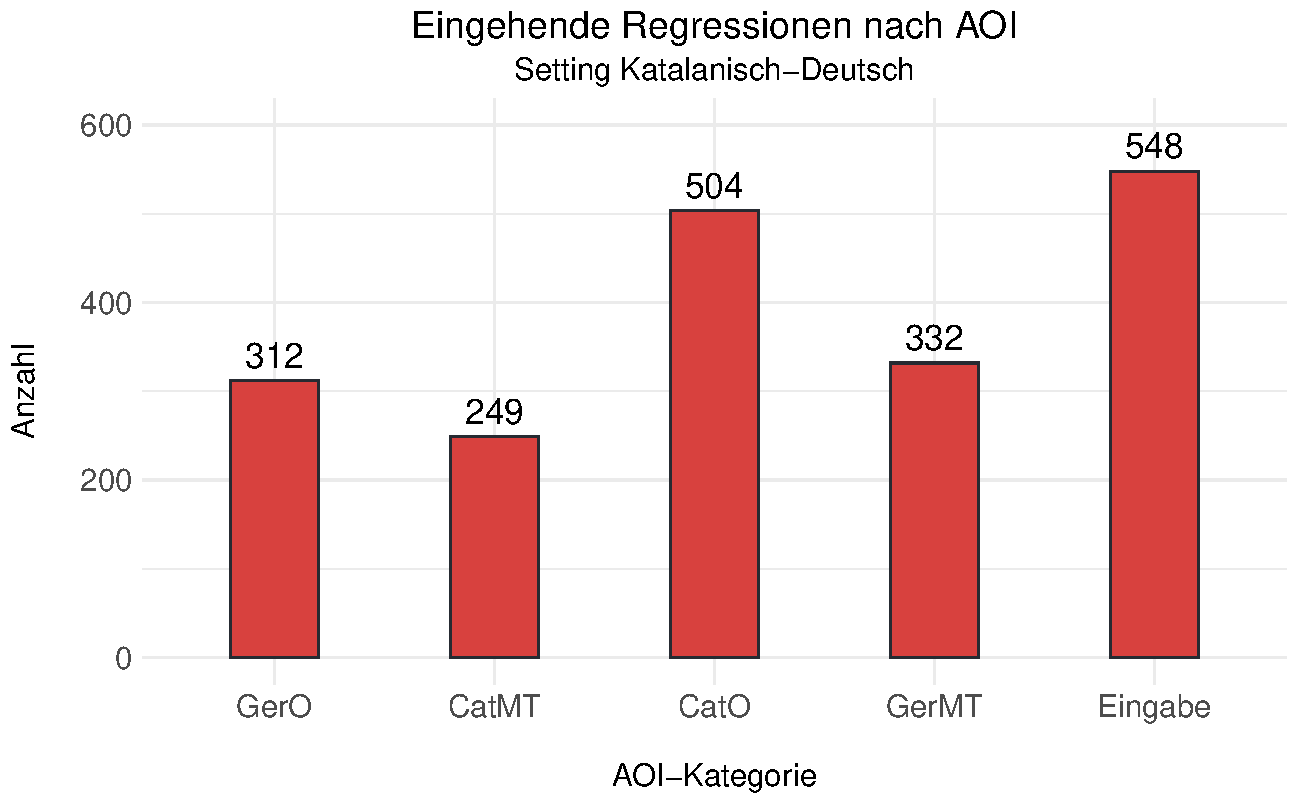
\includegraphics[width=.85\textwidth]{Figures/EyeTracking/CatDe/ggplot_regression_IN_AOI_de}
	\caption{Anzahl Regressionen in ein AOI}
	\label{K6:fig:CatDe:RegIn-AOI-Count}
\end{figure}

\begin{table}[p]
\begin{tabular}{lrS[table-format=2.2]S[table-format=2.2]} 
\lsptoprule
    {AOI-Kategorie} & \multicolumn{1}{c}{Summe} & {Mittelwert} & {SD} \\ 
    \midrule
    GerO  &  312 & 1,04 & 2,39 \\ 
    CatMT &  249 & 0,67 & 1,09 \\ 
    CatO & 504 & 1,16 & 1,53 \\ 
    GerMT &  332 & 0,65 & 1,07 \\ 
    Eingabe  & 548 & 26,1 & 14,6 \\ 
    \midrule
    Global &  1.945 & 1,19 & 3,61 \\ 
    \lspbottomrule
\end{tabular}
    \caption{Summe, Mittelwert und SD der eingehenden Regressionen pro AOI-Kategorie\label{K6:tab:CatDe:mean-sd-regin}}
\end{table}

Zur Untersuchung der Regressionen in ein AOI wurde mit einem binomialen logistischen Regressionsmodell\is{Regressionsmodell!binominales logistisches}\is{Statistik!Testverfahren!Regressionsmodell} mit gemischten Effekten\is{Effekt!gemischter} gearbeitet, das die Teilnehmer{\textperiodcentered}innen (\emph{SessionLabel}) als Zufallseffekte\is{Effekt!Zufalls-} beinhaltete (s. \tabref{K6:tab:CatDe:RegIn-Modell-Stats}). Die Variablen wurden in einer bedingten Vorwärtsauswahl in das Modell integriert. Das simpelste und zugleich genauste Modell erweist sich dabei ebenso wie einzelne Koeffizienten der integrierten Variablen als signifikant und liefert bessere Ergebnisse als ein einfaches lineares Regressionsmodell\is{Regressionsmodell!lineares}\is{Statistik!Testverfahren!Regressionsmodell} ($\chi^2(9) = 50,91, p < 0,001$). Zugleich zeigt sich, dass das Modell noch nicht optimal angepasst (C: 0,73, Somers' D\textsubscript{XY}: 0,46)\is{Somers' D\textsubscript{XY}|see{Statistik}}\is{Statistik!Testverfahren!Somers' D\textsubscript{XY}} ist. Daher wurden die Ergebnisse noch einmal mittels nicht-parametrischer Tests\is{Statistik!Testverfahren!nicht-parametrisches} auf Plausibilität überprüft.

%------------------------------------

\begin{table}
    \small\fittable{\begin{tabular}{l@{ }S[table-format=-1.5] S[table-format=1.7] S[table-format=2.2] S[table-format=2.5] S[table-format=-1.3] S[table-format=<1.6{***},table-align-text-after=false]} 
    \lsptoprule
                     & {Gruppen} & {Varianz} & {SD} & {L.R. X2} & {DF} & {Pr} \\\midrule
    Zufallseffekt(e) &	{SessionLabel} &	0,3167 &	0,5628 &	50,907 &	21 &	< 0,001{***}\\\midrule
    Fixe Effekt(e) &	{Schätzung} &	{VIF} &	{OR} &	{SE} &	{$z$} & {$\text{Pr}(>z)$} \\\midrule
    (Intercept) &	0,49460 &	&	1,59 &	0,52049 &	1,976 &	< 0,05{*}\\
    IATagCatO &	0,55883 &	1,6827326 & 1,70 &	0,16221 &	3,445 &	< 0,001{***}\\
    IATagEingabe &	4,85341 &	1,8523138 &	25,74 &	1,93224 &	2,512 &	< 0,05{*}\\
    IATagGerMT &	-0,16912 &	1,6189873 &	0,81 &	0,14887 &	-1,136 &	0,225943\\
    IATagGerO &	-0,09574 &	1,5730919 &	0,90 &	0,17642 &	-0,543 & 	0,587328 \\
    IAFFixPro1 &	-0,95428 &	1,1235513 &	0,37 &	0,14752 &	-6,469 &	< 0,001{***} \\
    IARegPD\_z &	-0,29912 &	1,9849059 &	0,84 &	0,10146 &	-2,948 &	< 0,01{**} \\
    IA\_AREA\_z &	0,29316 &	1,1041541 & 	1,42 &	0,06123 &	4,788 &	< 0,001{***} \\\lspbottomrule
    \end{tabular}}\medskip\\
    \begin{tabular}{lS[table-format=4.7]}\lsptoprule
    {Model statistics} &	\multicolumn{1}{c}{Wert}\\\midrule
    {No. Groups}  &	21 \\
    {Number of cases in model}  	&	1,636 \\
    {Observed misses}  	& \\	
    {Observed deviance} 	&	2021,0 \\
    {Residual deviance} 	&	\\
    {R2 (Nagelkerke)}	 	&	0,1212020 \\
    {R2 (McFadden)} 	 	&	0,0702412 \\
    {R2 (Cox \& Snell)}	&	0,891032 \\
    {C} 	&	0,7282527 \\
    {Somers' D\textsubscript{XY}} 	&		0,4565054 \\
    {AIC} 		&	2039,0 \\
    {BIC} 		&	2087,6 \\\midrule
    Prediction accuray & \\
    Model Likelihood Ratio Test\\
    x2: &  152,68\\
    df: & 7 \\
        & {p < 0,001} *** \\
        \lspbottomrule
    \end{tabular}
    \caption[Werte des Regressionsmodells für eingehende Regressionen]
            {Werte des Regressionsmodells für eingehende Regressionen im 
             Setting Katalanisch-Deutsch\label{K6:tab:CatDe:RegIn-Modell-Stats}}
\end{table}

%------------------------------------

Während die Kategorien \emph{GerO} bzw.\ \emph{GerMT} keinen signifikanten Einfluss auf die Wahrscheinlichkeit haben, dass eine Regression in ein AOI gemacht wird, steigt die relative Wahrscheinlichkeit bei \emph{Eingabe} und \emph{Intercept} (\emph{CatMT} in diesem Fall) um jeweils 2.474\,\% bzw. 59\,\%. Für die Kategorie \emph{CatO} steigt die relative Wahrscheinlichkeit, dass eine Regression in dieses AOI gemacht wird, um 70\,\%. Weiterhin steigt die Wahrscheinlichkeit um 42\,\% mit der Größe der AOI. Hingegen nimmt die relative Wahrscheinlichkeit mit jeder Einheit der \emph{IARegPD} um 16\,\% und mit jeder progressiven ersten Fixation\is{Fixation!progressive erste} um 63\,\% ab.\largerpage[-1]

Die zur Überprüfung durchgeführten Chi-Quadrat-Tests\is{Chi-Quadrat-Test|see{Statistik}}\is{Statistik!Testverfahren!Chi-Quadrat-Test} deuten ebenfalls in die von dem Modell aufgezeigte Richtung: Es besteht ein signifikanter Unterschied zwischen der jeweils betrachteten AOI-Kategorie\is{Area of Interest!Kategorie} und der eingehenden Regression\is{Regression!eingehende} ($\chi^2(4) = 72,56, p < 0,001$). Die progressive erste Fixation\is{Fixation!progressive erste} steht zudem ebenfalls in einem signifikanten Verhältnis zu den eingehenden Regressionen. Sowohl die statistische Untersuchung des globale Datensatzes ($\chi^2(1) = 99,38,\allowbreak\ p < 0,001$) als auch nach den Kategorien \emph{GerO} ($\chi^2(1) = 15,97, p < 0,001$), \emph{CatMT} ($\chi^2(1) = 26,16, p < 0,001$) und \emph{GerMT} ($\chi^2(1) = 27,84, p < 0,001$) weist signifikante Unterschiede auf. Die weiteren im Modell verwendeten Variablen führen hingegen zu keinerlei signifikantem Ergebnis.

\is{Regression!eingehende|)}


%------------------------------------------------------------------------

\subsubsubsection{Ausgehende Regressionen}
\label{K6:para:catde:regout}

%------------------------------------------------------------------------

\is{Regression!ausgehende|(}
\figref{K6:fig:CatDe:RegOut-AOI-Count} und \tabref{K6:tab:CatDe:mean-sd-regout} zeigen die aufsummierte Anzahl aller Regressionen\is{Regression!Summe aller} aus einem AOI nach Kategorie sowie deren Mittelwert und Standardabweichung. Aus der maschinellen Übersetzung ins Deutsche und ins Katalanische wurden dabei die meisten Regressionen (\emph{GerMT}: 627, \diameter\,1,23, SSD: 1,68 und \emph{CatMT}: 397, \diameter\,1,08, SD: 2,31) getätigt, die wenigsten Regressionen kamen aus dem AOI der Kategorie deutsches Original (\emph{GerO}: 45, \diameter\,0,15, SD: 0,46). Aus den Kategorien \emph{Eingabe} und katalanisches Original wurden jeweils 108 (\diameter\,5,14, SD: 11,71) bzw. 77 (\diameter\,0,18, SD: 0,64) Regressionen vorgenommen. Im Durchschnitt wird jeweils mindestens eine Regression aus den maschinell übersetzten Nachrichten ins Katalanische und ins Deutsche getätigt. Aus der Eingabemaske werden im Schnitt sogar fünf Regressionen ausgeführt, der absolute Wert liegt hier jedoch mit 108 im unteren Bereich.

%------------------------------------------------------------------------

\begin{figure}
	\centerline{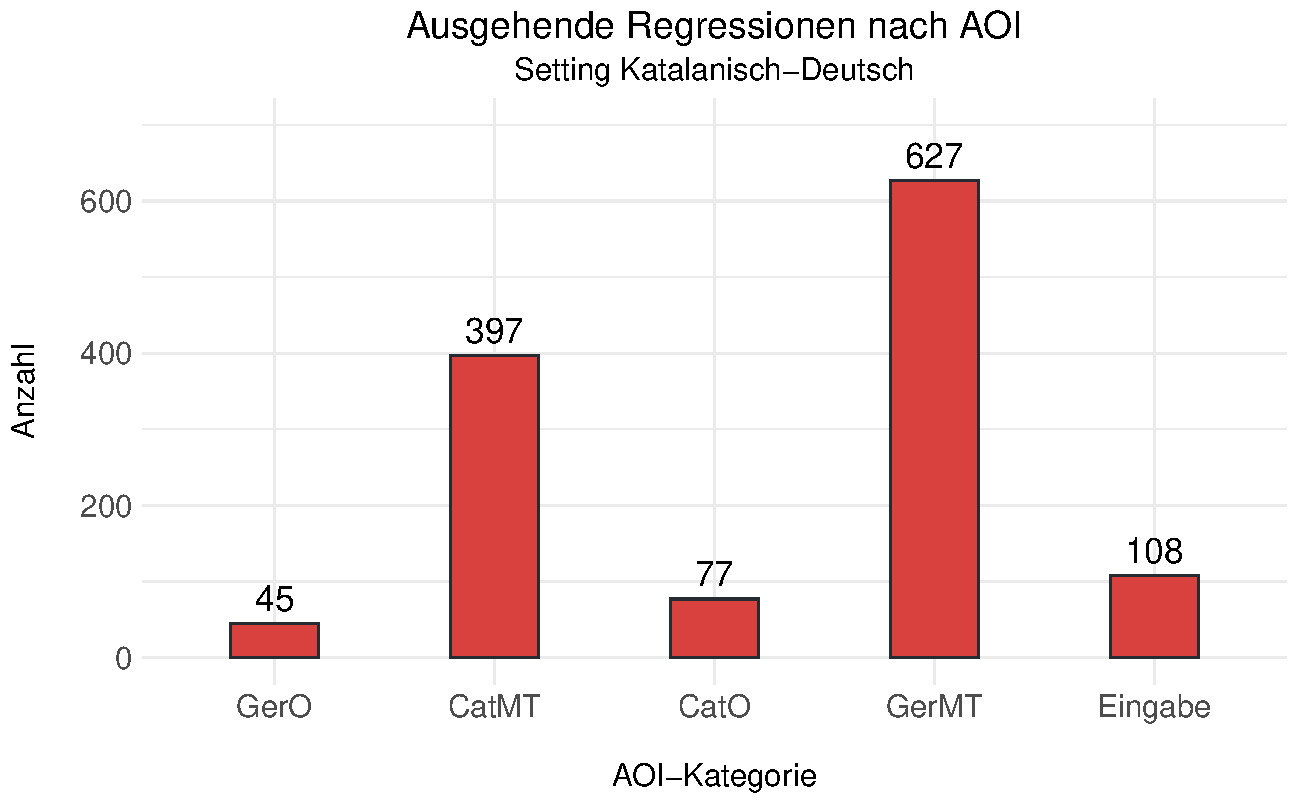
\includegraphics[width=.85\textwidth]{Figures/EyeTracking/CatDe/ggplot_regression_OUT_AOI_de}}
	\caption{Anzahl Regressionen aus einem AOI\label{K6:fig:CatDe:RegOut-AOI-Count}}
\end{figure}

%------------------------------------------------------------------------

%------------------------------------



\begin{table}
\begin{tabular}{lrS[table-format=2.2]S[table-format=2.2]} 
\lsptoprule
    {AOI-Kategorie} & \multicolumn{1}{c}{Summe} & {Mittelwert} & {SD} \\\midrule
    GerO  &  45 & 0,15 & 0,46 \\ 
    CatMT &  397 & 1,08 & 2,31 \\ 
    CatO & 77 & 0,18 & 0,64 \\ 
    GerMT &  627 & 1,23 & 1,68 \\ 
    Eingabe  &  108 & 5,14 & 11,71 \\\midrule
    Global &  1.254 & 0,77 & 2,1 \\ 
    \lspbottomrule
\end{tabular}
    \caption{Summe, Mittelwert und SD der ausgehenden Regressionen pro AOI-Kategorie\label{K6:tab:CatDe:mean-sd-regout}}
\end{table}

%------------------------------------

Zur Untersuchung der Regressionen aus einem AOI wurde mit einem binomialen logistischen Regressionsmodell\is{Regressionsmodell!binominales logistisches}\is{Statistik!Testverfahren!Regressionsmodell} mit gemischten Effekten\is{Effekt!gemischter} gearbeitet, das die Teilnehmer{\textperiodcentered}innen (\emph{SessionLabel}) als Zufallseffekte\is{Effekt!Zufalls-} beachtete (s. \tabref{K6:tab:CatDe:RegOut-Modell-Stats}). Die Variablen AOI-Kategorie\is{Area of Interest!Kategorie}, AOI-Größe\is{Area of Interest!Größe des}, progressive erste Fixation\is{Fixation!progressive erste}, Dauer des ersten Durchlaufs\is{Durchlauf!Dauer des ersten} und regressive Durchlaufdauer\is{Durchlauf!-dauer!regressive} wurden in einer bedingten Vorwärtsauswahl in das Modell integriert. Das simpelste und zugleich genauste Modell bietet dabei bessere Resultate als ein einfaches lineares Regressionsmodell\is{Regressionsmodell!lineares}\is{Statistik!Testverfahren!Regressionsmodell} ($\chi^2(9) = 191,82, p < 0,001$), erweist sich allerdings auch als nicht optimal angepasst (C: 0,90, Somers’ D\textsubscript{XY}: 0,80)\is{Statistik!Testverfahren!Somers' D\textsubscript{XY}}. Das endgültige, simpelste Modell zeigt signifikante Werte bei einzelnen Kategorien der unabhängigen Variable \emph{IATag}.\largerpage

%------------------------------------

\begin{table}[p]
    \small
    
    \fittable{\begin{tabular}{lS[table-format=-2.6]S[table-format=1.6]S[table-format=2.3]S[table-format=<2.5{***}]S[table-format=-1.4]S[table-format=<1.4{***}]} 
    \lsptoprule
         & {Gruppen} & {Varianz} & {SD} & {L.R. X2} & {DF} & {Pr}\\
        \midrule
    Zufallseffekte	& {SessionLabel} &	5,854 &	2,419 	&		< 0,001{***} \\\midrule
    Fixe Effekte &	{Schätzung} &	{VIF} &	{OR} &	{SE} &	{$z$} & {$\text{Pr}(> z)$}  \\\midrule
    (Intercept) &	-0,93610 &	&	0,794 &	0,55865 &	-1,676 &	0,0938{.} \\
    IATagCatO &	-1,21271 &	1,3833037 &	0,292 &	0,21022 &	-5,769 	& < 0,001{***} \\
    IATagEingabe &	-12,80930 &	1,0005803 &	0,000 &	57,24434 &	-0,224 &	0,8229 \\
    IATagGerMT &	0,91356 &	1,454387 &	1,933 &	0,17529 &	5,212 &	< 0,001{***} \\
    IATagGerO &	-1,09895 &	1,3365114 &	0,349 &	0,23442 &	-4,688 &	< 0,001{***}\\
    IA\_AREA\_z &	0,17517 &	1,1163253 &	0,988 &	0,08277 &	2,116 &	0,0343{*}\\
    IARegPD\_z &	4,36986 &	1,3180099 &	32,037 &	0,43993 &	9,933 &	< 0,001{***}\\
    IARunDwell\_z &	-0,31179 &	1,2305214 &	0,808 &	0,07934 &	-0,3930 &	< 0,001{***}\\
    \lspbottomrule
    \end{tabular}}\medskip\\
    \begin{tabular}{lS[table-format=<4.7{***}]}
    \lsptoprule
    {Model statistics} 						&	{Wert} \\\midrule
    {No. Groups} 						&	21 \\
    {Number of cases in model} 						&	1,636 \\
    {Observed misses} 						& \\	
    {Observed deviance} 						&	1366,8 \\
    {Residual deviance} 						&	\\
    {R2 (Nagelkerke)} 						&	0,452491 \\
    {R2 (McFadden)} 						&	0,314851 \\
    {R2 (Cox \& Snell)} 						&	0,318824 \\
    {C} 						&	0,9008282 \\
    {Somers' D\textsubscript{XY}} 					&		0,8016564 \\
    {AIC} 						&	1384,8 \\
    {BIC} 						&	1433,4 \\
    Prediction accuray & \\	
    Model Likelihood Ratio Test\\
    x2: & 628,12\\
    df: & 7\\
    $p$: & <0,001{***}\\
        \lspbottomrule
    \end{tabular}
    \caption[Werte des Regressionsmodells für ausgehende Regressionen]
            {Werte des Regressionsmodells für ausgehende Regressionen 
             im Setting Katalanisch-Deutsch\label{K6:tab:CatDe:RegOut-Modell-Stats}}
\end{table}

% 	\end{table}


%------------------------------------


Während Regressionen aus der Eingabemaske und aus dem \emph{Intercept} (\emph{CatMT} in diesem Fall) keinen bzw. nur einen marginalen Effekt auf die Wahrscheinlichkeit haben, dass eine Regression aus dem AOI gemacht wird, weisen die Kategorien \emph{GerMT}, \emph{GerO} und \emph{CatO} eine jeweils signifikante Wahrscheinlichkeit auf. Aus der Kategorie \emph{GerMT} steigt die Wahrscheinlichkeit um 93\,\%, aus den Kategorien \emph{GerO} und \emph{CatO} hingegen sinkt die relative Wahrscheinlichkeit um jeweils 65\,\% bzw. 71\,\%. Die Größe der AOI ist signifikant (p < 0,05), die Wahrscheinlichkeit einer Regression aus dem AOI sinkt mit einer Einheit um 1\,\%.

% %------------------------------------------------------------------------

% \begin{figure}[htbp]
% 	%\centering
% 	\centerline{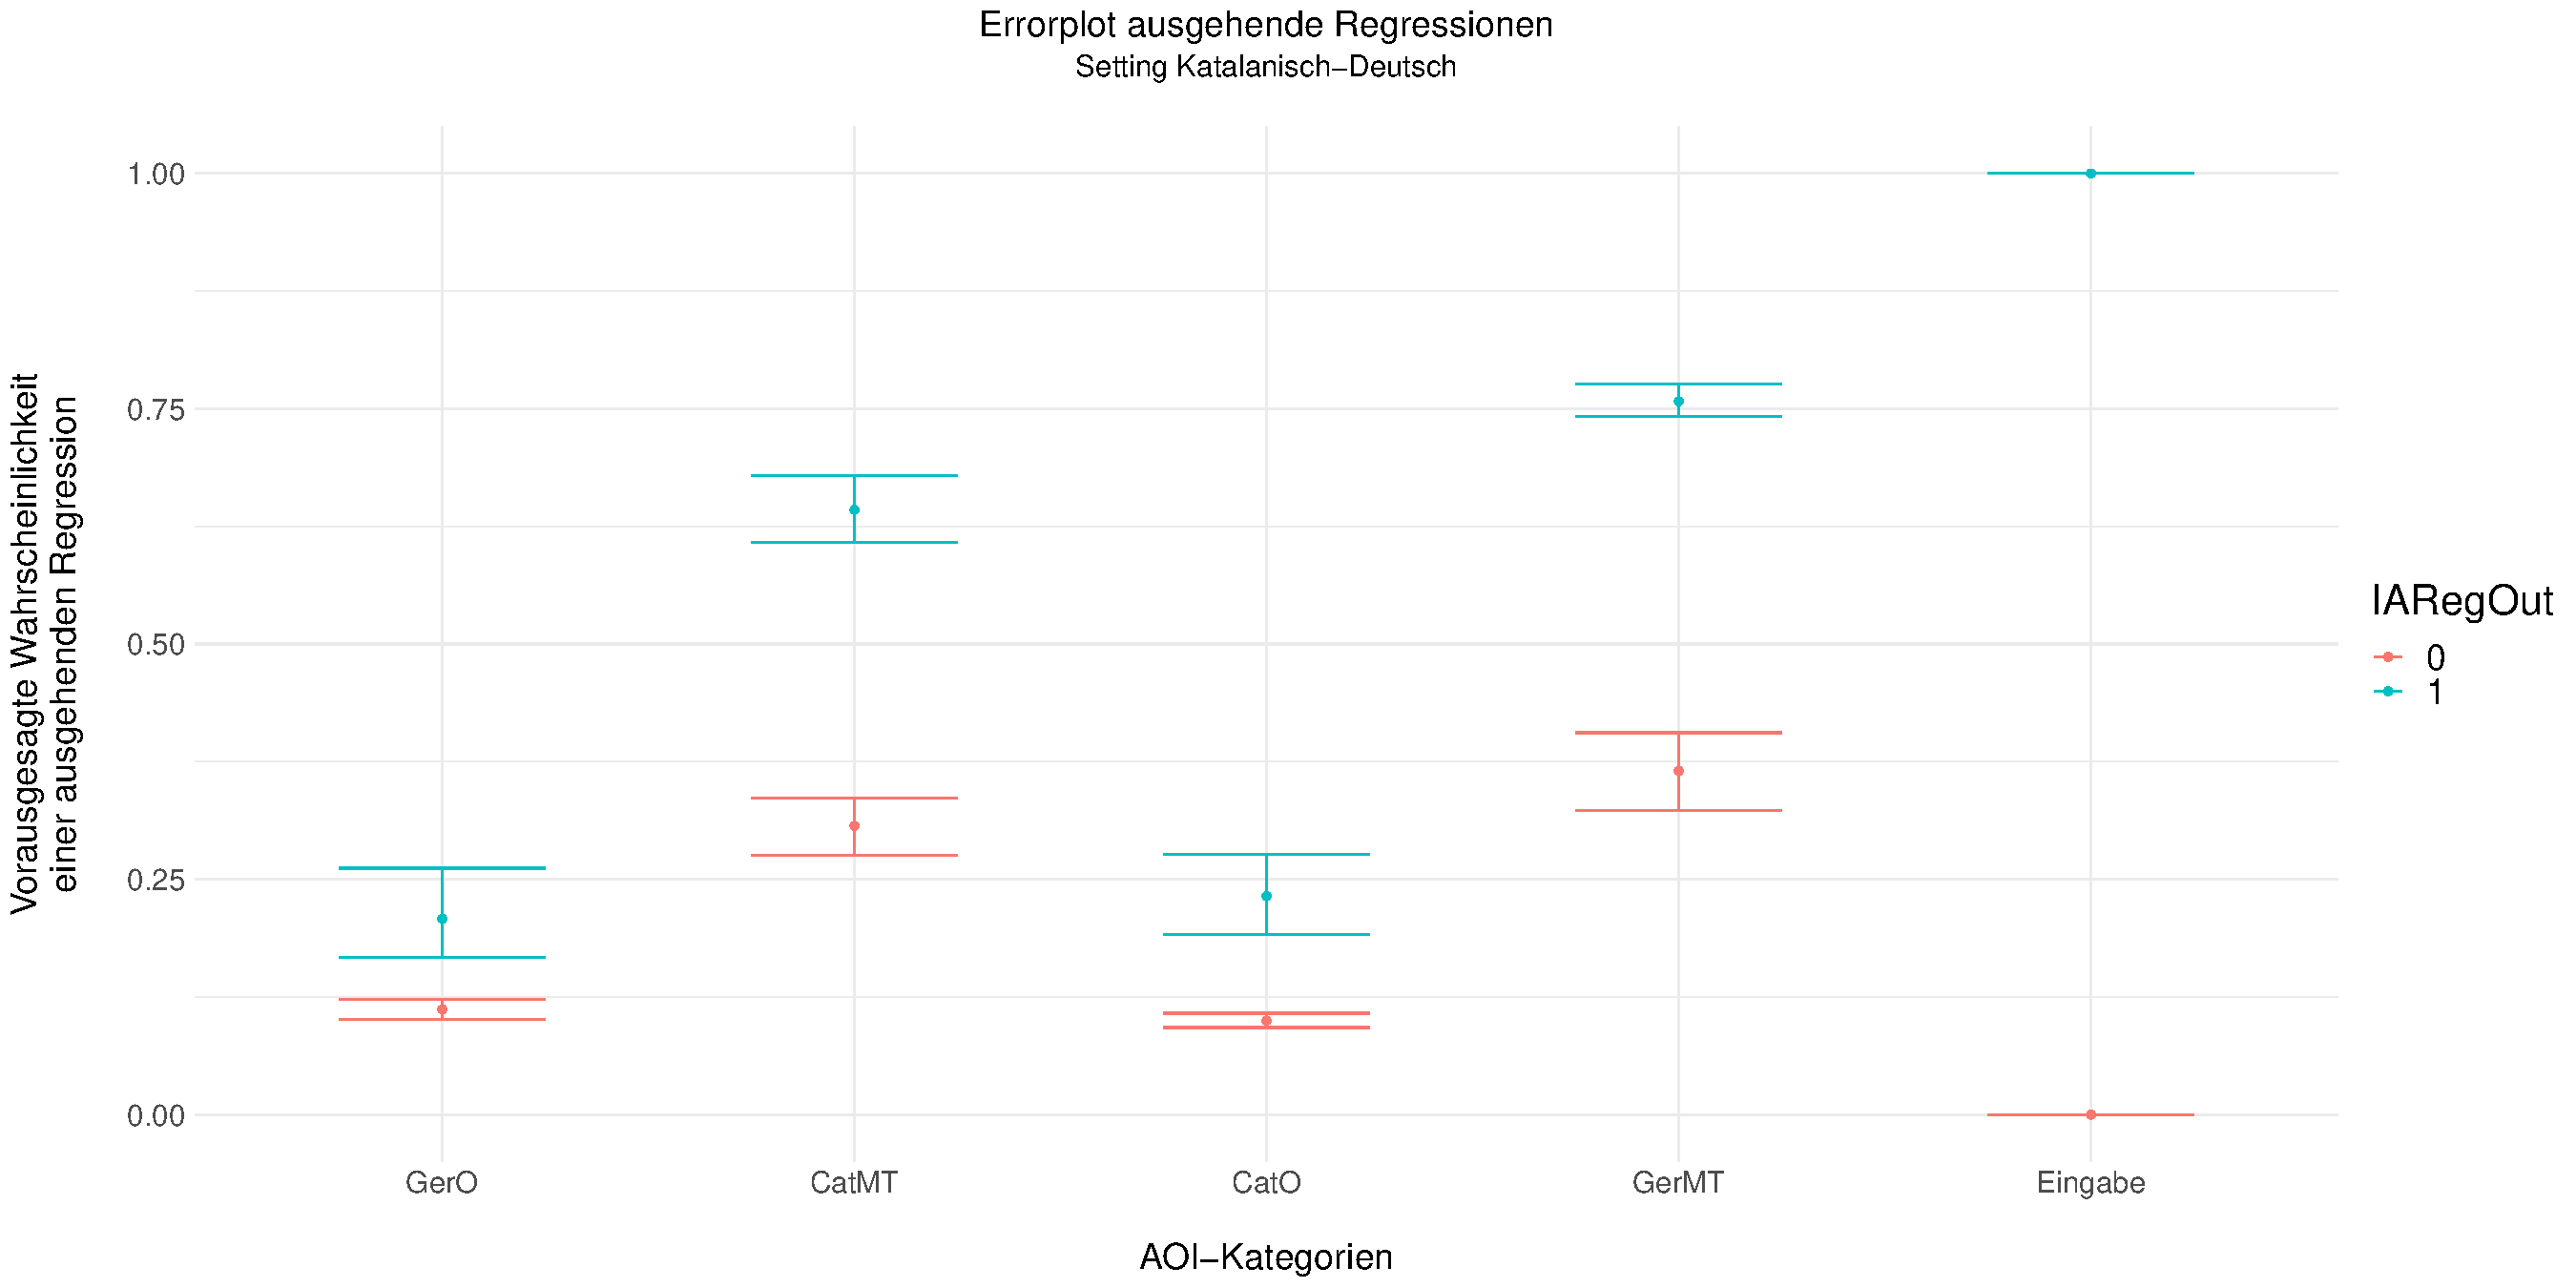
\includegraphics[width=\textwidth]{Figures/EyeTracking/CatDe/ggplot_errorplot-prob-regOut-CatDe}}
% 	\caption{Errorplot der Wahrscheinlichkeit für eine ausgehendeRegression}
% 	\label{K6:fig:CatDe:RegOut-Errorplot}
% \end{figure}

% %------------------------------------------------------------------------

Wie auch bei den eingehenden Regressionen wurde hier zur Überprüfung der Plausibilität mit Chi-Quadrat-Tests\is{Statistik!Testverfahren!Chi-Quadrat-Test} gearbeitet. So bestehen signifikante Unterschiede zwischen den ausgehenden Regressionen pro AOI-Kategorie ($\chi^2(4) = 331,16, p < 0,001$). Die progressive erste Fixation ergibt ebenfalls auffällige Ergebnisse. Der gesamte Datensatz ($\chi^2(1) = 454,2, p < 0,001$) sowie die gesonderte Betrachtung nach AOI-Kategorie \emph{GerO} ($\chi^2(1) = 43,25, p < 0,001$), \emph{CatMT} ($\chi^2(1) = 76,77, p < 0,001$), \emph{CatO} ($\chi^2(1) = 65,44, p < 0,001$) und \emph{GerMT} ($\chi^2(1) = 177,42, p < 0,001$) liefern hier signifikante Resultate. Alle weiteren im Modell verwendeten Variablen erweisen sich darüber hinaus als statistisch unauffällig.

\is{Regression!ausgehende|)}


%------------------------------------------------------------------------

\subsubsection{Dauer des ersten Durchlaufs}

\label{K6:subsubsec:iafrd:catde}

%------------------------------------------------------------------------
\begin{sloppypar}
\tabref{K6:tab:CatDe:mean-sd-iafrd} zeigt die aufsummierte Dauer des ersten Durchlaufs\is{Durchlauf!Dauer des ersten|(} pro AOI-Kategorie und die entsprechenden Mittelwerte sowie Standardabweichungen. Während die Durchlaufdauer innerhalb der Eingabemaske und den deutschen Originalnachrichten mit jeweils 10.728\,ms bzw. 179.586\,ms am kürzesten ist, erreicht der Durchlauf der MÜ ins Deutsche den Höchstwert von 391.664\,ms. Dies gilt ebenfalls für die durchschnittliche Zeit, die der erste Durchlauf pro AOI benötigt. Auch hier liegt die MÜ ins Deutsche mit 815,97\,ms deutlich über dem Schnitt von 641,98\,ms und auch dem deutschen Original mit 600,62\,ms. Die beiden katalanischsprachigen Beitragsarten liegen mit durchschnittlich 611,18\,ms (\emph{CatMT}) und 508,86\,ms (\emph{CatO}) hingegen unter dem Gesamtschnitt. Die jeweilige Gesamtdurchlaufdauer liegt zwischen der des deutschen Originals und der der MÜ ins Deutsche.
\end{sloppypar}

%------------------------------------

\begin{table}
    \begin{tabular}{lrrrr}  
    \lsptoprule
        {AOI-Kategorie} & \multicolumn{1}{c}{Summe} & \multicolumn{1}{c}{Mittelwert} & \multicolumn{1}{c}{Median} & \multicolumn{1}{c}{SD} \\
        \midrule
        GerO   & 179.586 & 600,62 & 427,0 & 562,68 \\ 
        CatMT   & 221.246 & 611,18 & 426,5 & 558,06 \\ 
        CatO 	& 218.808 & 508,86 & 380,0 & 451,91 \\ 
        GerMT	& 391.664 & 815,97 & 513,0 & 738,49\\ 
        Eingabe   & 10.728 & 510,86 & 335,0 & 643,96 \\ 
        \midrule
        Global  & 1.022.032 & 641,98 & 427,0 & 607,56\\ 
        \lspbottomrule
    \end{tabular}
        \caption[Summe, Mittelwert, Median und SD der Dauer des ersten Durchlaufs]{Summe, Mittelwert, Median und SD der Dauer des ersten Durchlaufs in ms pro AOI-Kategorie\label{K6:tab:CatDe:mean-sd-iafrd}}
\end{table}

%------------------------------------

%------------------------------------------------------------------------

\begin{figure}
    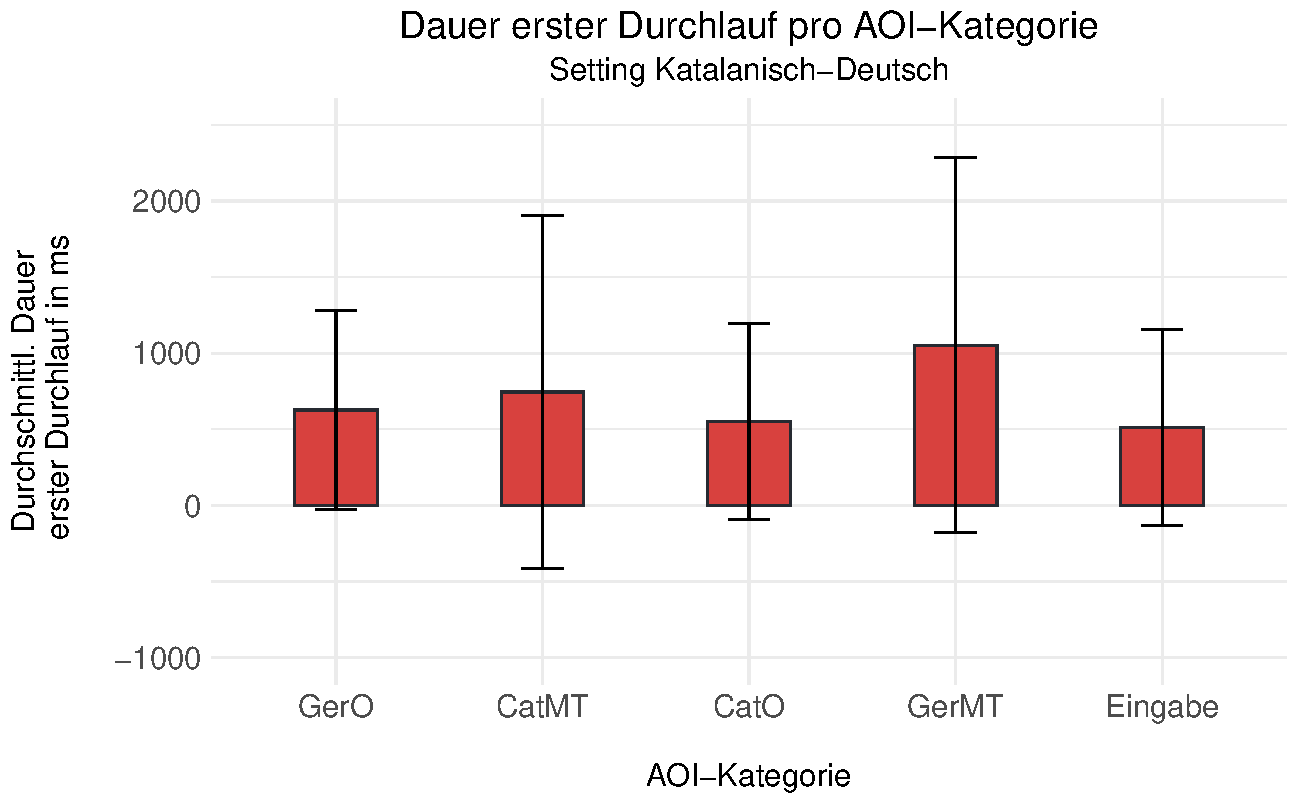
\includegraphics[width=\textwidth]{Figures/EyeTracking/CatDe/ggplot_catde_meanfrundwell_AOI_de}
	\caption{Durchschnittliche Betrachtungsdauer im ersten Durchlauf pro AOI-Kategorie im Setting Katalanisch-Deutsch}
	\label{K6:fig:CatDe:mean-error-FRDwell}
\end{figure}

%------------------------------------------------------------------------

Wie die graphische Inspektion des Datensatzes anhand von \figref{K6:fig:CatDe:IAFRD_density} darstellt, kann nicht von einer Normalverteilung ausgegangen werden. Eine logarithmische Transformation (rechte Seite der Abbildung) ändert nichts an dieser Beobachtung. Auch die statistische Untersuchung des Datensatzes mittels Shapiro-Wilk-Test\is{Statistik!Testverfahren!Shapiro-Wilk-Test}\is{Shapiro-Wilk-Test|see{Statistik}} lehnt die Annahme einer Normalverteilung ab (roh: $W = 0,79, p < 0,001$ und log10: $W = 0,98, p < 0,001$).


%------------------------------------------------------------------------

\begin{figure}
    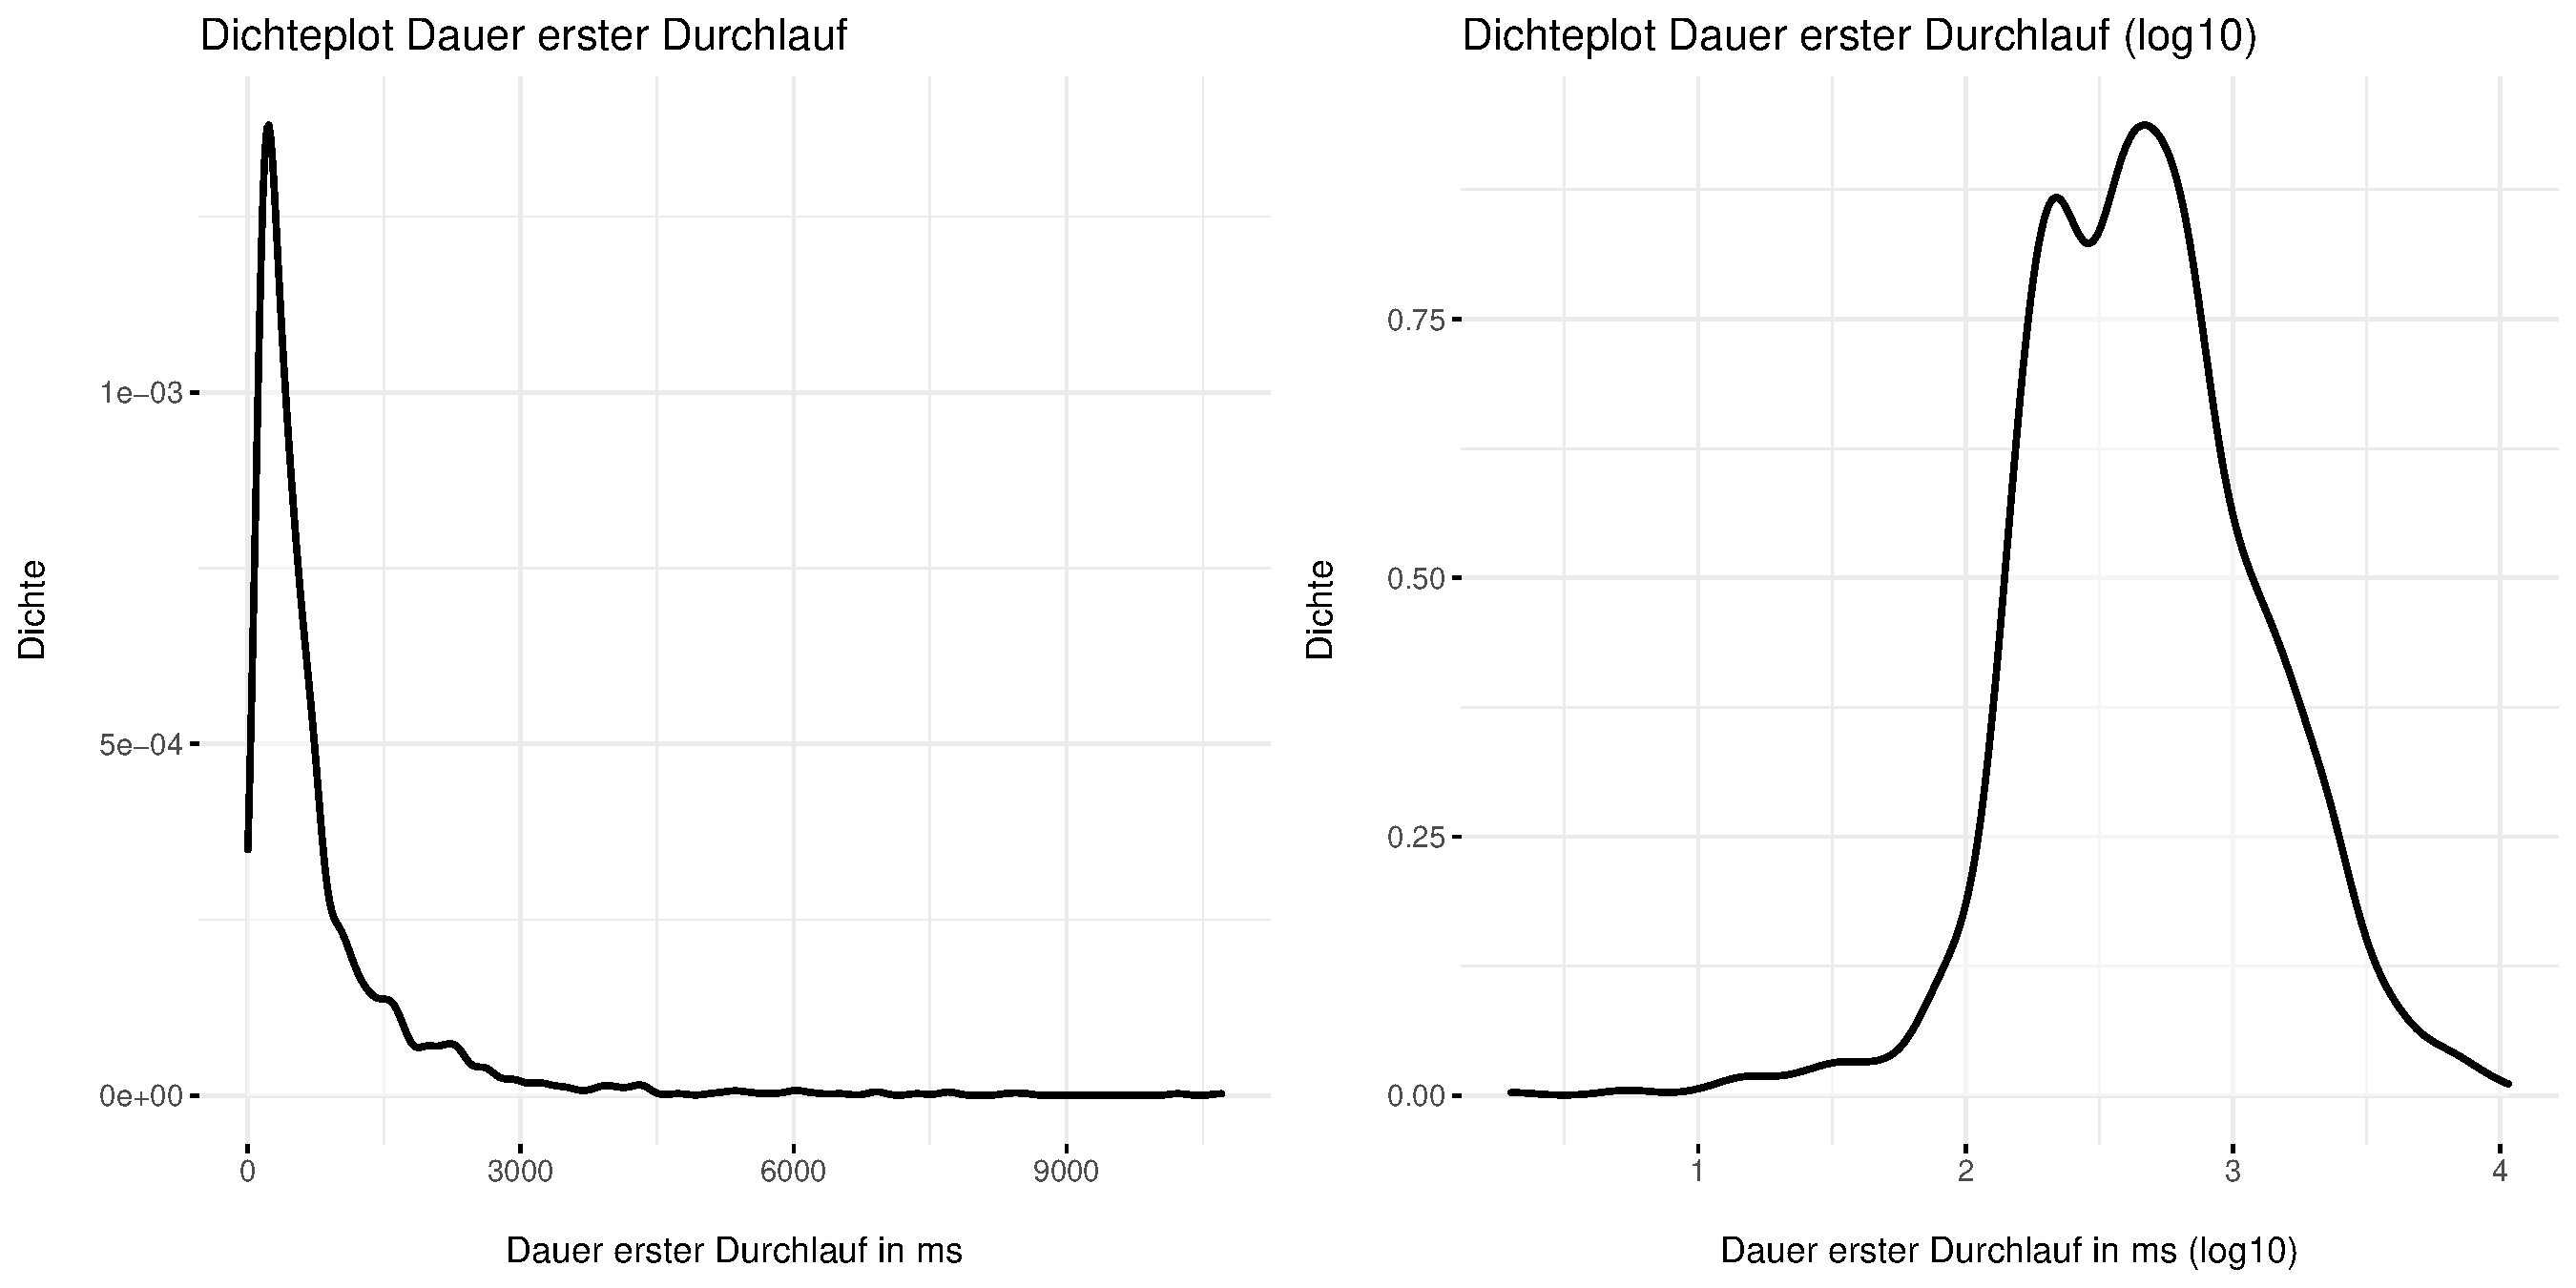
\includegraphics[width=\textwidth]{Figures/EyeTracking/CatDe/ggplot_CatDe-FRDwell_density_de}
	\caption{Verteilung der Betrachtungsdauer im ersten Durchlauf in ms: normal (links), logarithmisch transformiert (rechts)}
	\label{K6:fig:CatDe:IAFRD_density}
\end{figure}

%------------------------------------------------------------------------

Ein Kruskal-Wallis-Test\is{Statistik!Testverfahren!Kruskal-Wallis-Test} bestätigt, dass Unterschiede in der zentralen Tendenz der Betrachtungsdauer im ersten Durchlauf pro AOI zwischen den einzelnen Teilnehmer{\textperiodcentered}innen bestehen ($\chi^2(20) = 85,85, p < 0,01$). Anschließend durchgeführte Post-hoc-Tests (Dunn-Benjamini-Hochberg-Tests)\is{Statistik!Testverfahren!Dunn-Benjamini-Hochberg-Test} zeigen, dass sich 70 von 210 TN-Gruppen (33,33\,\%) signifikant unterscheiden, sodass gefolgert werden kann, dass die Dauer im ersten Durchlauf in gewissem Maße von der Individualität der TN abhängt.

Ein weiterer Kruskal-Wallis-Test\is{Statistik!Testverfahren!Kruskal-Wallis-Test} ergibt, dass Unterschiede in der zentralen Tendenz der Dauer des ersten Durchlaufs zwischen den einzelnen AOI-Ka\-te\-go\-ri\-en bestehen ($\chi^2(4) = 34,05, p < 0,01$). Anschließend durchgeführte Post-hoc-Tests (Dunn-Benjamini-Hochberg-Tests)\is{Dunn-Benjamini-Hochberg-Test}\is{Statistik!Testverfahren!Dunn-Benjamini-Hochberg-Test} zeigen, dass sich vor allem die Gruppierungen mit Beteiligung der maschinellen Übersetzung ins Deutsche (\emph{CatMT-GerMT}, \emph{CatO-GerMT}, \emph{Eingabe-GerMT} sowie \emph{GerMT-GerO}) unterscheiden, sodass gefolgert werden kann, dass die Durchlaufdauer von der AOI-Kategorie, und speziell von der Richtung (ins Deutsche), abhängt (s. \tabref{K6:tab:CatDe:dunntest-iafrd}). Die Effektstärke nach \citet{cohen_power_1992}\is{Effektstärke nach Cohen|see{Statistik}}\is{Statistik!Testverfahren!Effektstärke nach Cohen} liegt bei allen Gruppierungen nur im schwachen Bereich.

%------------------------------------



\begin{table}
\begin{tabular}{lS[table-format=-1.6]S[table-format=1.4]@{ }lS[table-format=1.2]}
\lsptoprule
    {AOI-Kategoriepaar} & {$z$} & \multicolumn{2}{c}{$p$ (angepasst)} & {Effekt}\\ 
    \midrule
    CatMT-CatO    &  1,851890 & 0,640 & \\
    CatMT-Eingabe &  1,467788 & 0,1015 &  \\
    CatO-Eingabe  & 0,883115 & 0,2095 & \\
    CatMT-GerMT   & -3,294221 & 0,0016 & **   & 0,11 \\
    CatO-GerMT    & -5,442975 & 0,0000 & ***  & 0,20 \\
    Eingabe-GerMT & -2,506379 & 0,0152 & *    & 0,11 \\
    CatMT-GerO    &  0,223453 & 0,4116 & \\
    CatO-GerO     & -1,522364 & 0,1066 &  \\
    Eingabe-GerO  &  -1,382031 & 0,1044 &  \\
    GerMT-GerO    &  3,349606 & 0,0020 & ** & 0,12 \\
    \lspbottomrule
\end{tabular}
    \caption{Ergebnisse des Dunn-Tests: Gruppierte Vergleiche der Dauer des ersten Durchlaufs nach AOI-Kategorie\label{K6:tab:CatDe:dunntest-iafrd}}
\end{table}

%------------------------------------

Weiterhin wurden die Unterschiede in der Dauer des ersten Durchlaufs zwischen den beiden Ausprägungen der progressiven ersten Fixation\is{Fixation!progressive erste}\is{first fixation progressive} untersucht. Da die progressive erste Fixation nur in zwei Ausprägungen vorliegt (0 und 1), wird nicht der Kruskal-Wallis-Test, sondern der Mann-Whitney-U-Test\is{Statistik!Testverfahren!Mann-Whitney-U-Test} verwendet. Es besteht allerdings kein signifikanter Unterschied in der zentralen Tendenz der Dauer des ersten Durchlaufs zwischen den AOI, bei denen zuvor ein AOI mit höherer Ordnungszahl betrachtet wurde, und denen, die chronologisch betreten wurden. Die Testergebnisse des gesamten Datensatzes und der einzelnen AOI-Kategorien sind in der \tabref{K6:tab:CatDe:mwu-ffixpro-iafrd} aufgeführt.

%------------------------------------


\begin{table}	
    \begin{tabular}{lccc}  
    \lsptoprule
        {AOI-Kategorie} & {$U$} & {$p$ (angepasst)} & {$r$}\\ 
        \midrule
        GerO &  24.004,0 & 0,23 & 0,07 \\
        CatMT & 13.022,5 & 0,61 & 0,03\\
        CatO & 50.083,5 & 0,81 & 0,01 \\
        GerMT & 24.098,0 & 0,30 & 0,05 \\
        \midrule
        Gesamt & 437.979,5 & 0,58 & 0,01 \\
        \lspbottomrule
        
    \end{tabular}
        \caption[Ergebnisse des Mann-Whitney-U-Tests zur Dauer des ersten Durchlaufs]{Ergebnisse des Mann-Whitney-U-Tests zur Dauer des ersten Durchlaufs nach progressiver erster Fixation und AOI-Kategorie}
    \label{K6:tab:CatDe:mwu-ffixpro-iafrd}
\end{table}

%------------------------------------

Die Dauer der Fixationen im ersten Durchlauf korreliert signifikant mit der Größe der AOI ($r_{s} = 0,10, p < 0,01, n = 602.248.371$)\is{Spearman's Rho}\is{Korrelationstest nach Spearman|see{Statistik}}\is{Statistik!Testverfahren!Korrelationstest nach Spearman}. Dabei handelt es sich nach \citet{cohen_power_1992}\is{Statistik!Testverfahren!Effektstärke nach Cohen} um einen schwachen Effekt. Das Bestimmtheitsmaß beträgt 1,09\,\%.
\is{Durchlauf!Dauer des ersten|)}



%------------------------------------------------------------------------

\subsubsection{Gesamtverweildauer}

\label{K6:subsubsec:dwelltime:catde}

%------------------------------------------------------------------------

\is{Verweildauer!Gesamt-|(}
In \tabref{K6:tab:CatDe:mean-sd-dwell} (S.\,\pageref{K6:tab:CatDe:mean-sd-dwell}) sind die Summe sowie die Mittelwert und Standardabweichung der Gesamtverweildauer in Millisekunden pro AOI-Kategorie dargestellt. Neben der Eingabemaske (12.000\,ms) verzeichnen die deutschsprachigen Originalbeiträge die niedrigste Summe (667.000\,ms). 

Im Vergleich dazu ist die Dauer im Falle der MÜ ins Katalanische beinahe doppelt so lang (1.305.000\,ms) bzw. im Falle der MÜ ins Deutsche sogar drei Mal so lang (1.944.000\,ms). Die aufsummierte Gesamtdauer beträgt 4.848.000\,ms. Die Werte der Eingabemaske lassen allerdings vermuten, dass es sich um einen Messfehler handelt oder die statische Annotation des AOI die Werte verzerrt. Auch mit Rückgriff auf die visuelle Inspektion, bei der sich eindeutig die Aufmerksamkeit auf den Bereich der Eingabemaske sowie leicht darüber konzentriert, l"asst sich nur so der Mittelwert von etwa 5.800\,ms bei einer aufsummierten Dauer von etwa 12.000\,ms und einer Standardabweichung von 8.000 erklären.

%------------------------------------

\begin{table}
    \begin{tabular}{lrrrr}
    \lsptoprule
        {AOI-Kategorie} & \multicolumn{1}{c}{Summe} & \multicolumn{1}{c}{Mittelwert} & \multicolumn{1}{c}{Median} & \multicolumn{1}{c}{SD} \\ 
        \midrule
        GerO & 666.787  & 2.230,06 & 1.137,0 & 3.311,21 \\ 
        CatMT & 1.305.425  & 3.596,21 & 2.005,0 & 4.219,83 \\ 
        CatO  & 919.508 & 2.123,58 & 1.038,0 & 3.081,15 \\ 
        GerMT & 1.944.324  & 3.865,46 & 2.766,0 & 3.815,79 \\ 
        Eingabe & 11.954 & 5.977,00 & 5.977,0 & 8.066,67 \\ 
        \midrule
        Global & 4.847.998 &  3.030,0 & 1.728,5 & 3.727,83 \\ 
        \lspbottomrule
    \end{tabular}
        \caption[Summe, Mittelwert, Median und SD der Gesamtverweildauer]{Summe, Mittelwert, Median und SD der Gesamtverweildauer in ms pro AOI-Kategorie}
    \label{K6:tab:CatDe:mean-sd-dwell}
\end{table}

%------------------------------------


%------------------------------------------------------------------------

\begin{figure}
    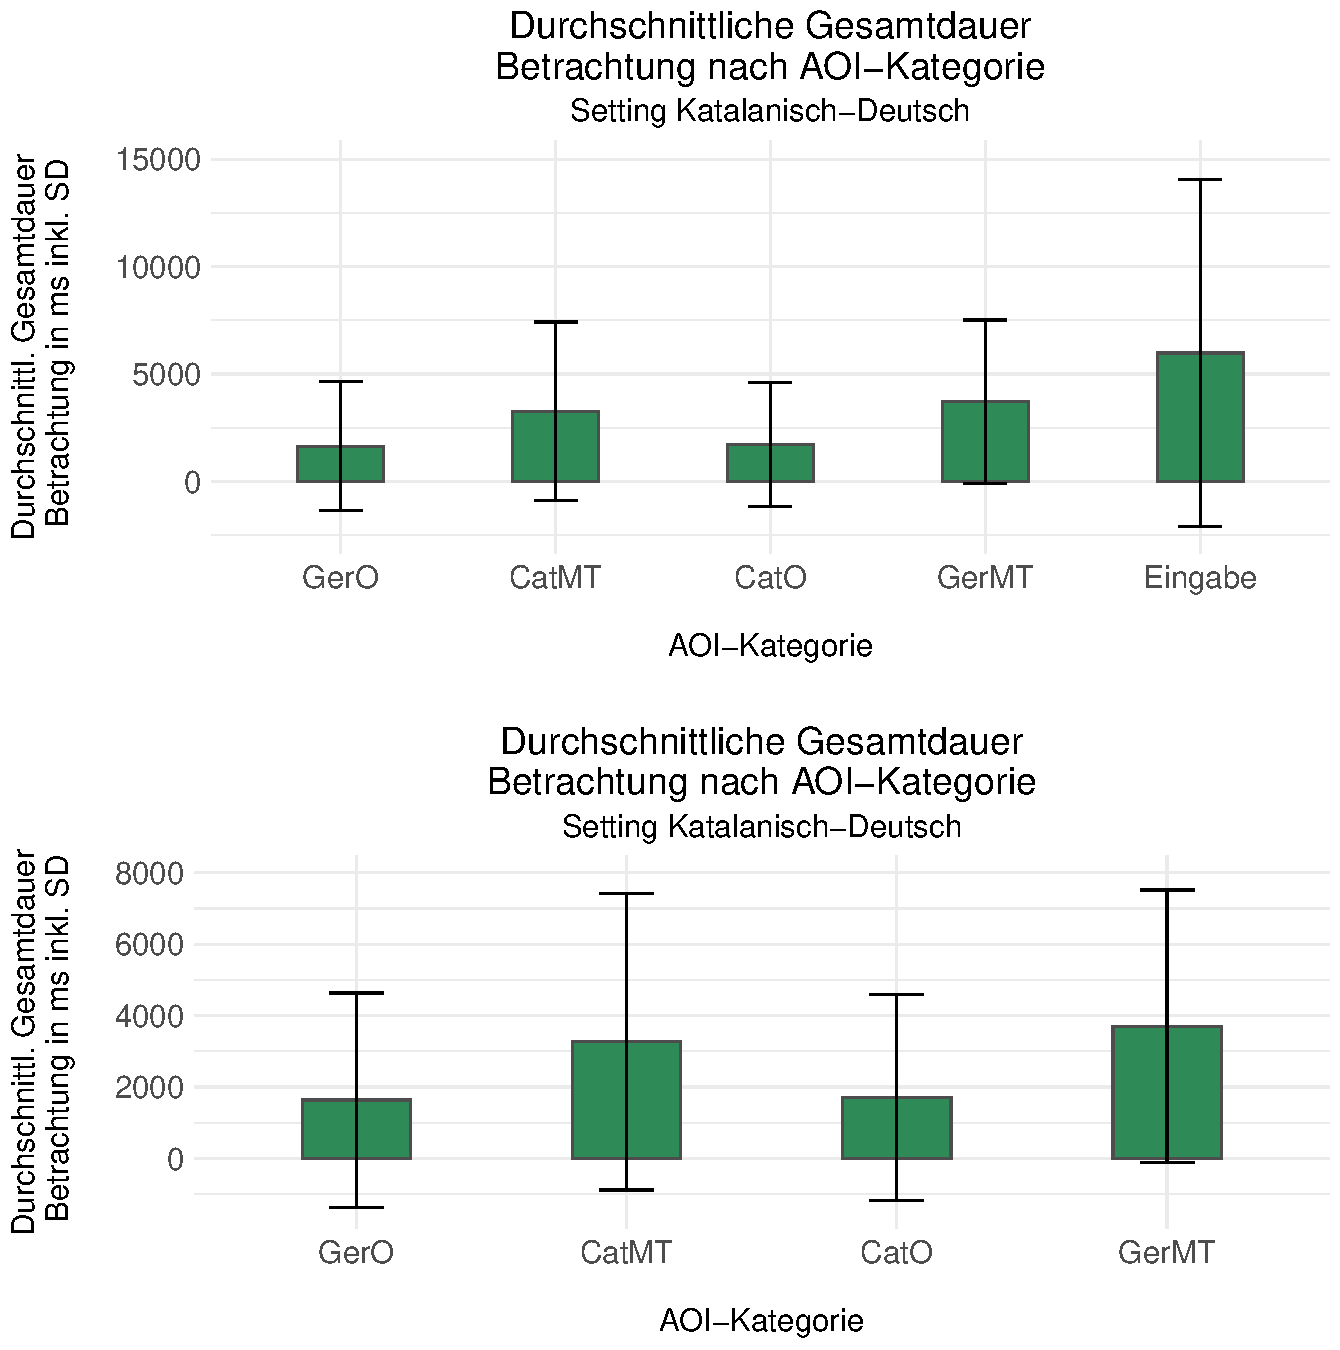
\includegraphics[width=\textwidth]{Figures/EyeTracking/CatDe/ggplot_catde_mean-dwell_AOI-grid-arrange_de}
	\caption{Durchschnittliche Betrachtungsdauer pro AOI-Kategorie im Setting Katalanisch-Deutsch, mit (oben) und ohne (unten) Eingabemaske\label{K6:fig:CatDe:mean-error-dwell}}
\end{figure}

%------------------------------------------------------------------------

Wie die graphische Inspektion des Datensatzes anhand von \figref{K6:fig:CatDe:density-dwell} andeutet, kann nicht von einer Normalverteilung ausgegangen werden. Eine logarithmische Transformation\is{Statistik!Transformation!logarithmische}\is{Transformation!logarithmische|see{Statistik}} (rechte Seite der Abbildung) ändert nichts an dieser Beobachtung. Auch die statistische Untersuchung des Datensatzes mittels Shapiro-Wilk-Test\is{Statistik!Testverfahren!Shapiro-Wilk-Test} lehnt die Annahme einer Normalverteilung ab (roh: $W = 0,69, p < 0,001$ und log10: $W = 0,995, p < 0,001$).

%------------------------------------------------------------------------

\begin{figure}
    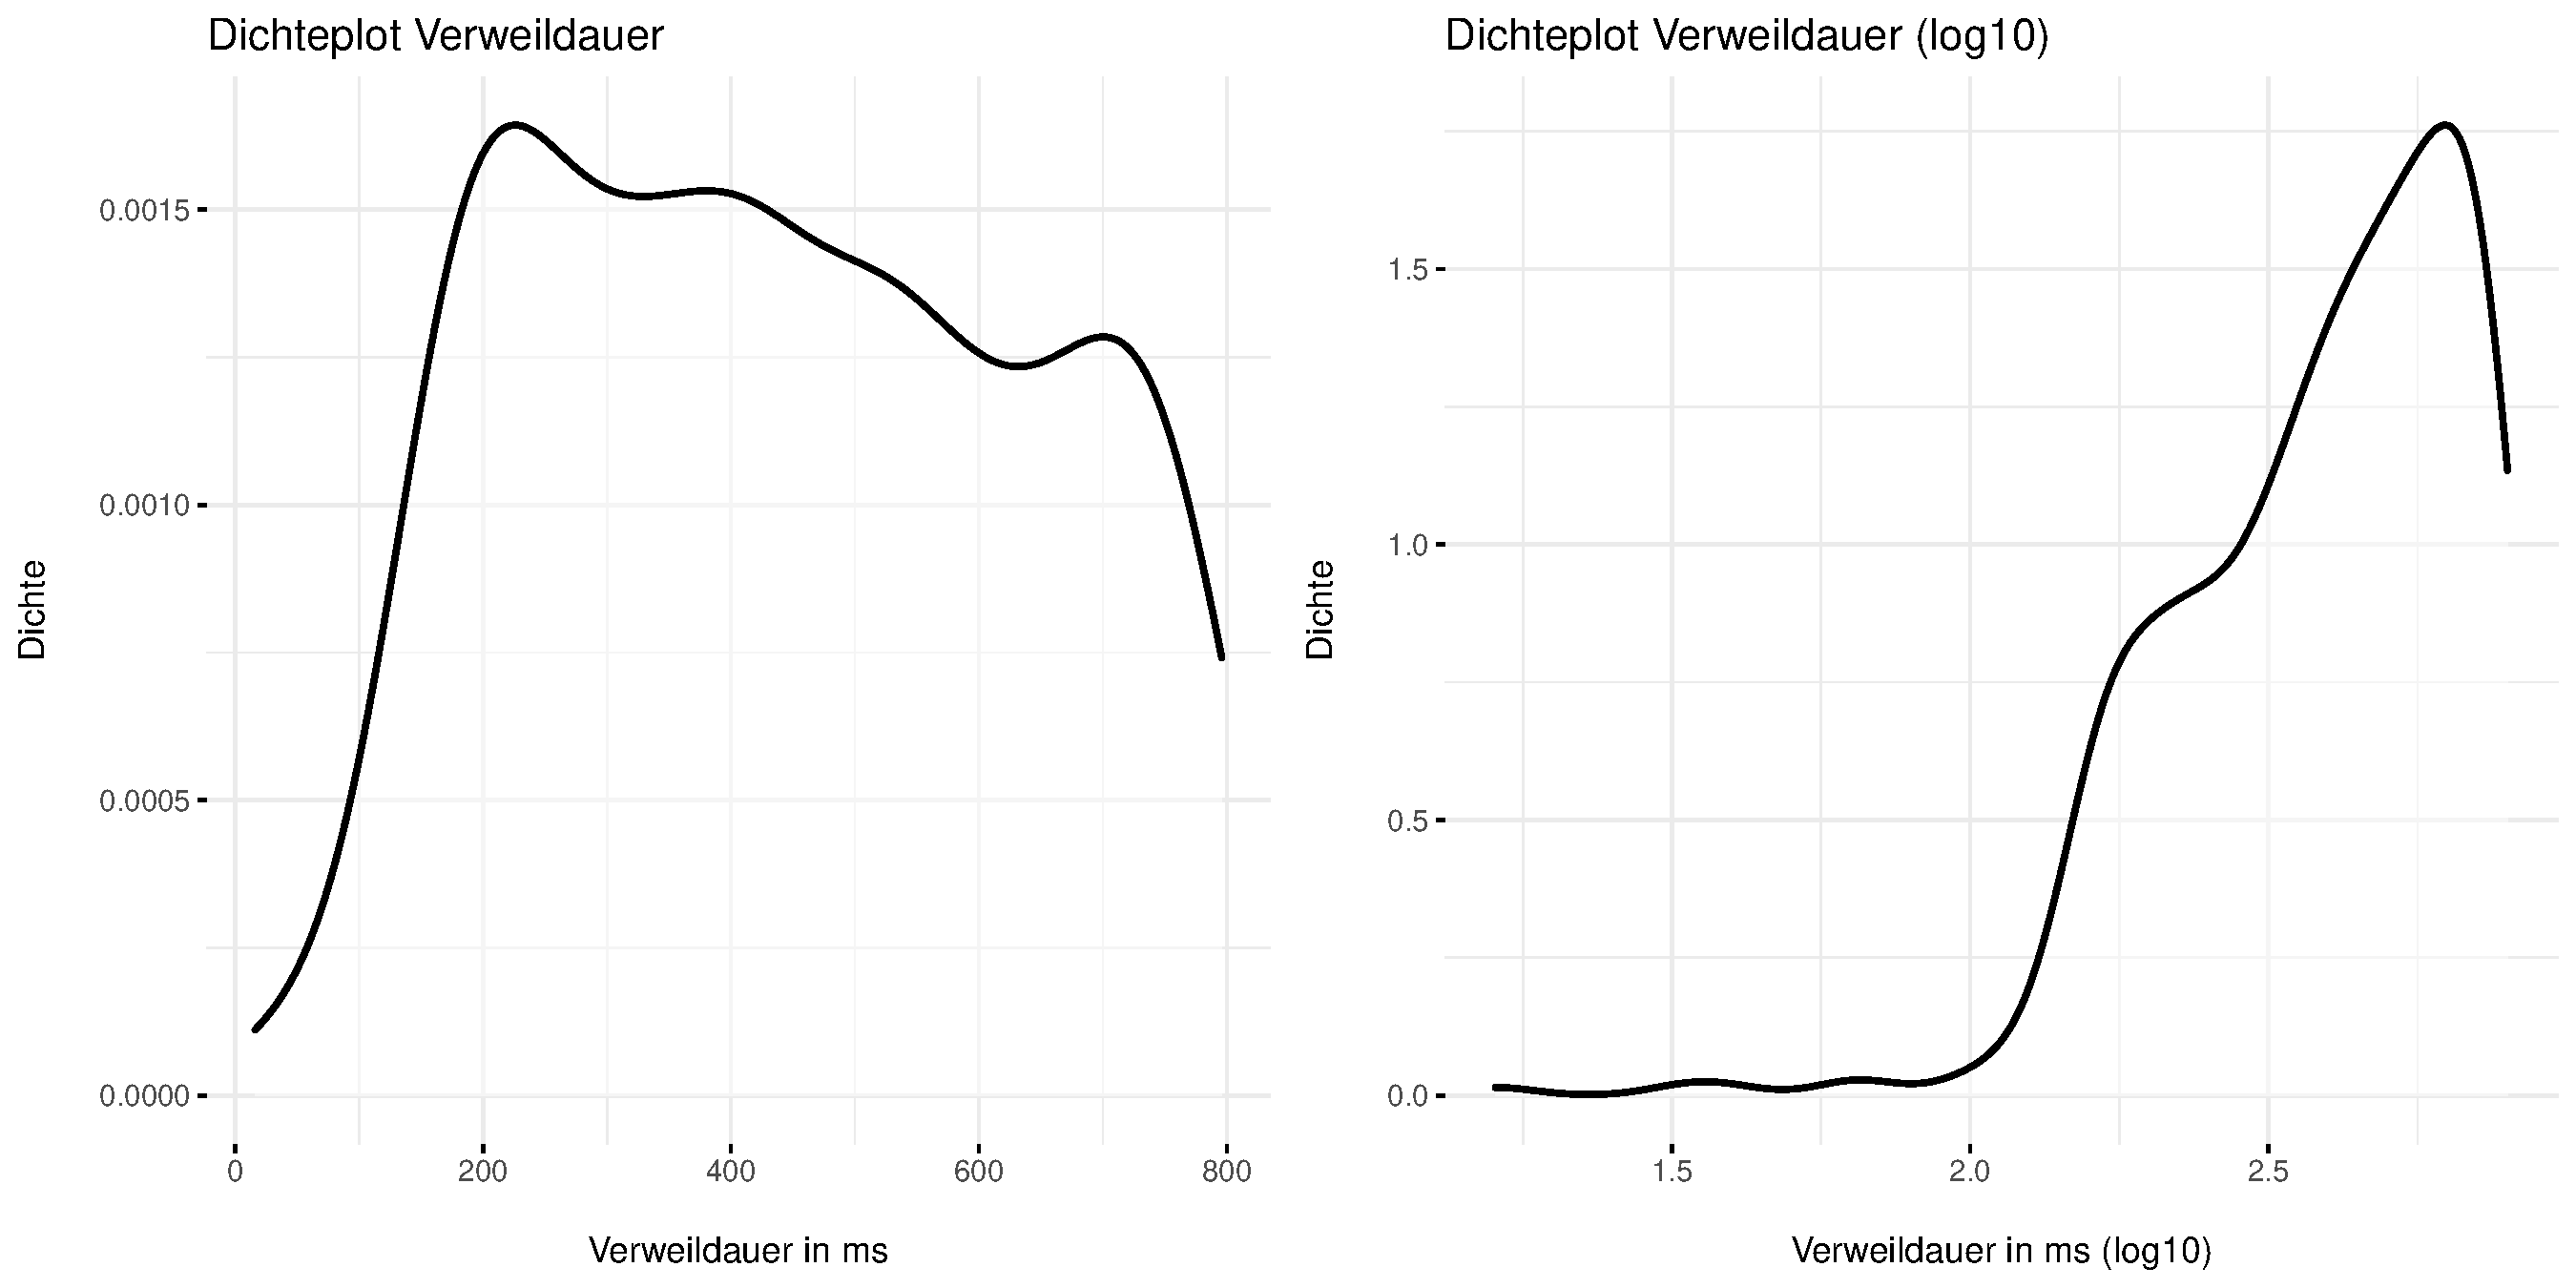
\includegraphics[width=\textwidth]{Figures/EyeTracking/CatDe/ggplot_catde-Dwell_density_de}
	\caption{Verteilung der Betrachtungsdauer in ms: normal (links), logarithmisch transformiert (rechts)}
	\label{K6:fig:CatDe:density-dwell}
\end{figure}

%------------------------------------------------------------------------

Ein Kruskal-Wallis-Test\is{Statistik!Testverfahren!Kruskal-Wallis-Test} belegt, dass Unterschiede in der zentralen Tendenz bei der Gesamtdauer der Betrachtung der AOI zwischen den einzelnen Teilnehmer{\textperiodcentered}innen bestehen ($\chi^2(20) = 213,34, p < 0,01$). Anschließend durchgeführte Post-hoc-Tests (Dunn-Benjamini-Hochberg-Tests)\is{Statistik!Testverfahren!Dunn-Benjamini-Hochberg-Test} zeigen, dass sich 129 von 210 TN-Gruppen (61,43\,\%) signifikant unterscheiden. Es kann demnach gefolgert werden, dass die Betrachtungsdauer in gewissem Maße von der Individualität der TN abhängt.

Ein zweiter Kruskal-Wallis-Test\is{Statistik!Testverfahren!Kruskal-Wallis-Test} deutet darauf hin, dass Unterschiede bei der Gesamtbetrachtungsdauer pro AOI zwischen den einzelnen AOI-Kategorien bestehen ($\chi^2(4) = 170,7, p < 0,01$). Anschließend durchgeführte Post-hoc-Tests (Dunn-Benjamini-Hochberg-Tests, s. \tabref{K6:tab:CatDe:dunntest-dwell})\is{Statistik!Testverfahren!Dunn-Benjamini-Hochberg-Test} zeigen, dass sich vor allem die Gruppierungen mit Beteiligung der maschinellen Übersetzung (\emph{CatMT-CatO}, \emph{CatMT-GerMT}, \emph{CatO-GerMT}, \emph{CatMT-GerO} sowie \emph{GerMT-GerO}) unterscheiden, sodass gefolgert werden kann, dass die Betrachtungsdauer von der AOI-Kategorie, und speziell von der Richtung, abhängt.

%------------------------------------

\begin{table}
    \begin{tabular}{lS[table-format=-2.6]S[table-format=1.4]@{ }lS[table-format=1.2]}  
    \lsptoprule
        {AOI-Kategoriepaar} & {$z$} & \multicolumn{2}{c}{$p$ (angepasst)} & {Effekt}\\ 
        \midrule
        CatMT-CatO    &  7,721200 &0,0000 & *** & 0,27 \\
        CatMT-Eingabe &  0,179601 &0,4287 & &\\
        CatO-Eingabe  & -0,595598 &0,3939 & &\\
        CatMT-GerMT   & -2,812706 &0,0049 & ** & 0,1 \\
        CatO-GerMT    & -11,33659 &0,0000 & *** & 0,37 \\
        Eingabe-GerMT & -0,453139 &0,3614 & &\\
        CatMT-GerO    &  6,331929 &0,0000 & *** & 0,25 \\
        CatO-GerO     & -0,730907 &0,3874 & &\\
        Eingabe-GerO  &  0,517520 &0,3780 & &\\
        GerMT-GerO    &  9,424509 &0,0000 & *** & 0,33 \\
        \lspbottomrule
    \end{tabular}
        \caption{Ergebnisse des Dunn-Tests: Gruppierte Vergleiche der Gesamtverweildauer nach AOI-Kategorie\label{K6:tab:CatDe:dunntest-dwell}}
\end{table}

%------------------------------------

Außerdem wurden die Unterschiede in der Gesamtbetrachtungsdauer nach progressiver erster Fixation\is{Fixation!progressive erste} untersucht. Da die progressive erste Fixation nur in zwei Ausprägungen vorliegt (0 und 1), wird nicht der Kruskal-Wallis-Test, sondern der Mann-Whitney-U-Test\is{Statistik!Testverfahren!Mann-Whitney-U-Test} verwendet. Es besteht ein signifikanter Unterschied in der zentralen Tendenz der Betrachtungsdauer zwischen den AOI, bei denen zuvor ein AOI mit höherer Ordnungszahl betrachtet wurde, und denen, die chronologisch betreten wurden (s.\ \tabref{K6:tab:CatDe:mwutest-dwell-ffixpro}).

%------------------------------------

	\begin{table}
		\begin{tabular}{lrS[table-format=1.3]@{ }lS[table-format=1.2]}  
		\lsptoprule
			{AOI-Kategorie} & \multicolumn{1}{c}{$U$} & \multicolumn{2}{c}{$p$ (angepasst)} & {Effekt}\\ 
			\midrule
			GerO    & 21.197,0 & 0,019 & * & 0,14 \\ 
			CatMT   & 10.987,0  & 0,015 & * & 0,13 \\ 
			CatO    & 46.146,0  & 0,001 & ** & 0,18 \\ 
			GerMT   & 22.032,5  & 0,092 & & \\ 
			Eingabe & 3,0       & 0,023 & * & 0,5 \\
			\midrule
			Global & 364.732,5 & 0,001 & ** & 0,23 \\ 
			\lspbottomrule			
		\end{tabular}
			\caption[Ergebnisse des Mann-Whitney-U-Tests zur Gesamtverweildauer]{Ergebnisse des Mann-Whitney-U-Tests zur Gesamtverweildauer und progressiven ersten Fixation nach AOI-Kategorie\label{K6:tab:CatDe:mwutest-dwell-ffixpro}}
	\end{table}


%------------------------------------

Die Durchlaufdauer korreliert signifikant mit der Größe der AOI ($r_{s} = 0,45, p < 0,01, n = 374.884.161$)\is{Spearman's Rho}\is{Korrelationstest nach Spearman}\is{Statistik!Testverfahren!Korrelationstest nach Spearman}. Dabei handelt es sich nach \citet{cohen_power_1992}\is{Statistik!Testverfahren!Effektstärke nach Cohen} um einen schwachen Effekt. Das Bestimmtheitsmaß beträgt 20,33\,\%.
\is{Verweildauer!Gesamt-|)}


%------------------------------------------------------------------------

\subsubsection{Regressive Durchlaufdauer}

\label{K6:subsubsec:regpd:catde}

%------------------------------------------------------------------------

\is{Durchlauf!-dauer!regressive|(}\is{regressive Durchlaufdauer|see{Durchlauf}}
\begin{sloppypar}
\tabref{K6:tab:CatDe:mean-sd-iaregpd} zeigt die Summe, Mittelwerte sowie die Standardabweichung der regressiven Durchlaufdauer in Millisekunden pro AOI-Kategorie. Während die Originalbeiträge im Deutschen insgsamt lediglich 397.000\,ms fixiert werden, beträgt die aufsummierte regressive Durchlaufdauer bei der MÜ ins Deutsche 3.244.000\,ms. Die MÜ wird in dieser Kategorie insgesamt also beinahe acht Mal so lange betrachtet. Auch die Durchlaufdauer des katalanischen Originals und der MÜ ins Katalanische unterscheidet sich etwa um den Faktor vier. Während das katalanische Original 695.000\,ms lang betrachtet wird, liegt der Wert bei der MÜ in die Sprache bei etwa 2.533.000 ms. Insgesamt beträgt die regressive Durchlaufdauer 8.064.000\,ms bzw. im Schnitt 4.929\,ms.
\end{sloppypar}

Auch die Mittelwerte unterscheiden sich deutlich. So beträgt die durchschnittliche regressive Durchlaufdauer für die deutschen Originalbeiträge 1.318\,ms, die der MÜ ins Deutsche hingegen 6.360\,ms. ähnlich unterschiedlich sind die Werte für die katalanischsprachigen Beiträge. Die regressive Durchlaufdauer beträgt für die katalanischen Originale durchschnittlich 1.600\,ms und für die MÜ in die Sprache 6.870\,ms. Somit liegen die jeweiligen Originalbeiträge um etwa den Faktor fünf unter der Durchlaufdauer der MÜ. Während der absolute Höchstwert bei der MÜ ins Deutsche liegt, findet sich der höchste Schnitt bei der MÜ ins Katalanische.

Die Eingabemaske wurde als statisches AOI annotiert. Der hohe Mittelwert erklärt sich daher aus dem anfänglichen Warteverhalten der Versuchspersonen bis der katalanische Gegenüber die erste Nachricht gesendet hat. Bis zu diesem Zeitpunkt verweilten die Proband{\textperiodcentered}innen meist sehr lange auf der Eingabemaske und damit innerhalb des AOI.

Eine graphische Inspektion der Daten (\figref{K6:fig:CatDe:density-iaregpd}) zeigt, dass weder die rohen noch die logarithmisch transformierten Werte\is{Statistik!Transformation!logarithmische} normalverteilt sind. Auch die statistische Untersuchung unter Anwendung des Shapiro-Wilk-Tests\is{Statistik!Testverfahren!Shapiro-Wilk-Test} deutet auf nicht normalverteilte Daten hin (roh: $W = 0,18, p < 0,001$, log10: $W = 0,99,\allowbreak\ p < 0,001$). Daher wird die regressive Durchlaufdauer mit nicht-parametrischen Tests\is{Statistik!Testverfahren!nicht-parametrisches} untersucht.

%------------------------------------

\begin{table}
    \begin{tabular}{lrrrr}  
    \lsptoprule
        {AOI-Kategorie} & \multicolumn{1}{c}{Summe} & \multicolumn{1}{c}{Mittelwert} & \multicolumn{1}{c}{Median} & \multicolumn{1}{c}{SD} \\ 
        \midrule
        GerO   & 396.755 & 1.318,12 & 802,0 & 1.831,13 \\ 
        CatMT   & 2.532.654 & 6.863,56 & 3.292,0 & 11.960,89 \\ 
        CatO 	& 694.504 & 1.596,56 & 710,0 & 3.244,24 \\ 
        GerMT	& 3.243.600 & 6.360,00 & 4.360,5 &  7.708,70\\ 
        Eingabe   & 1.196.802 & 56.990,57 & 2053,0 & 128.990,12 \\ 
        \midrule
        Global  & 8.064.315 & 4.929,29 & 1.789,0 & 17.299,95\\ 
        \lspbottomrule
    \end{tabular}
        \caption[Summe, Mittelwert, Median und SD der regressiven Durchlaufdauer]{Summe, Mittelwert, Median und SD der regressiven Durchlaufdauer in ms pro AOI-Kategorie\label{K6:tab:CatDe:mean-sd-iaregpd}}
\end{table}
	


%------------------------------------



%------------------------------------------------------------------------

\begin{figure}
    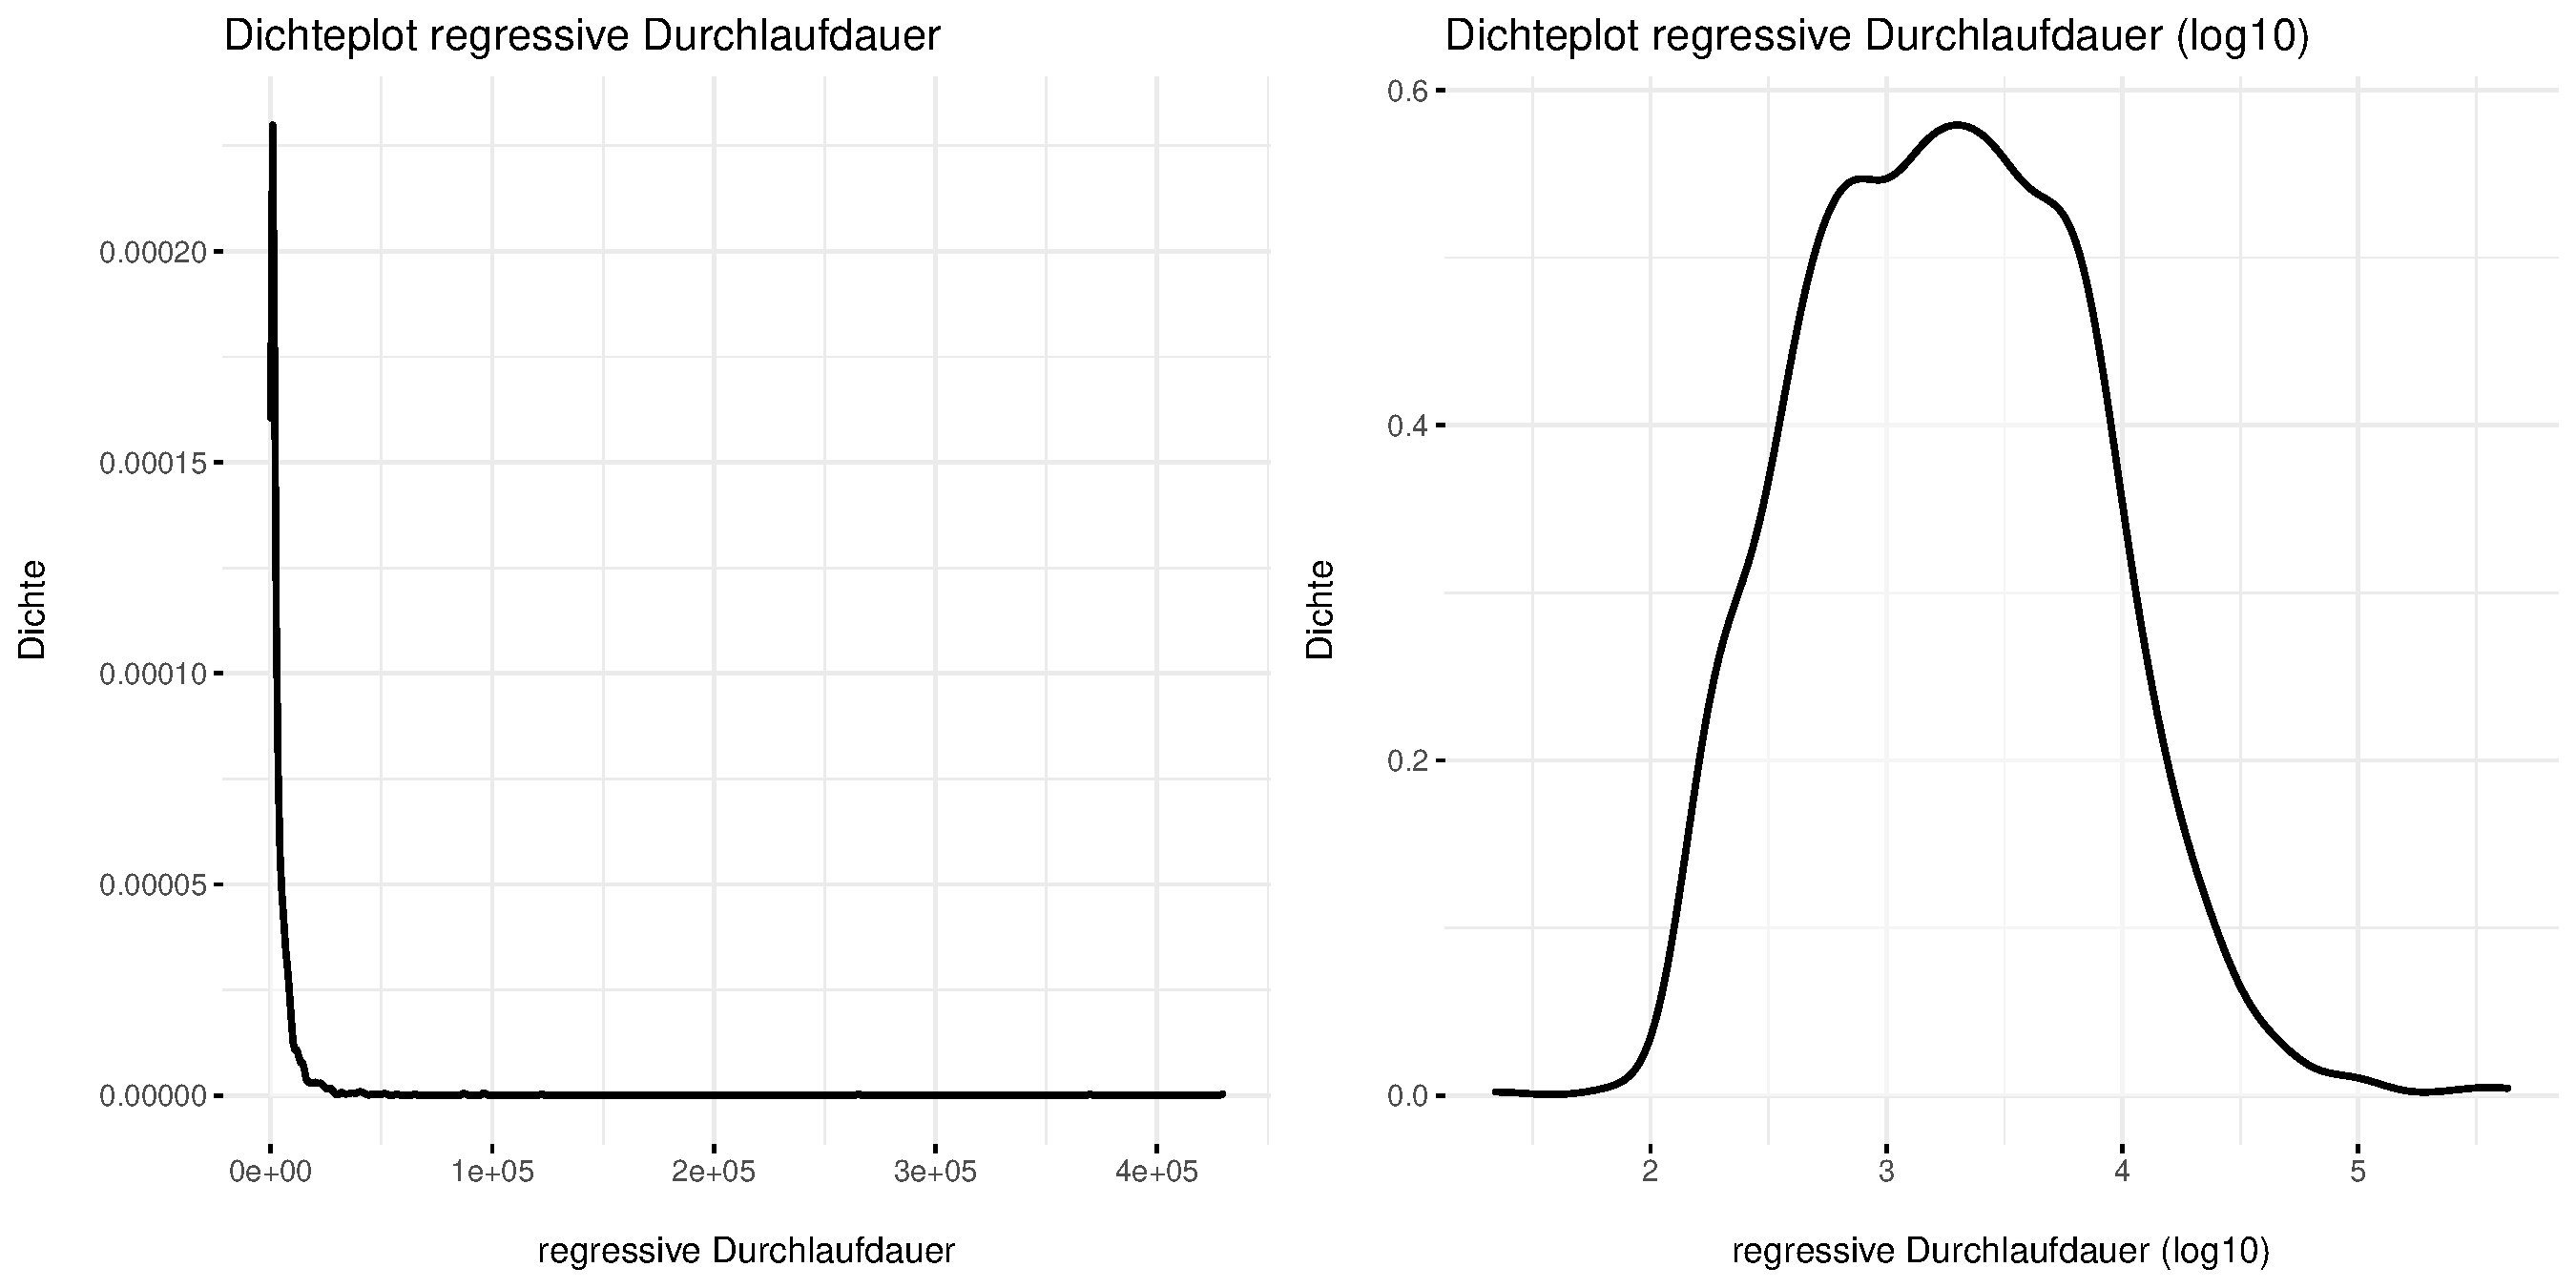
\includegraphics[width=\textwidth]{Figures/EyeTracking/CatDe/ggplot_catde-RegPD_density_de}
	\caption{Verteilung regressive Durchlaufdauer: normal (links), logarithmisch transformiert (rechts)}
	\label{K6:fig:CatDe:density-iaregpd}
\end{figure}

%------------------------------------------------------------------------

\begin{sloppypar}
Ein Kruskal-Wallis-Test\is{Statistik!Testverfahren!Kruskal-Wallis-Test} belegt, dass Unterschiede in der zentralen Tendenz der regressiven Durchlaufdauer pro AOI zwischen den einzelnen Teilnehmer{\textperiodcentered}innen bestehen ($\chi^2(20) = 81,83, p < 0,05$). Anschließend durchgeführte Post-hoc-Tests (Dunn-Benjamini-Hochberg-Tests)\is{Statistik!Testverfahren!Dunn-Benjamini-Hochberg-Test} zeigen, dass sich 61 von 210 TN-Gruppen (29,05\,\%) signifikant unterscheiden.
\end{sloppypar}

Ein zweiter Kruskal-Wallis-Test\is{Statistik!Testverfahren!Kruskal-Wallis-Test} zeigt zudem, dass Unterschiede in der zentralen Tendenz der regressiven Durchlaufdauer pro AOI zwischen den einzelnen AOI-Kategorien bestehen ($\chi^2(4) = 498,67, p < 0,05$). Anschließend durchgeführte Post-hoc-Tests (Dunn-Benjamini-Hochberg-Tests, \tabref{K6:tab:CatDe:dunntest-RegPD})\is{Statistik!Testverfahren!Dunn-Benjamini-Hochberg-Test} zeigen, dass sich alle außer die Gruppierungen \emph{CatO-GerO} und \emph{CatMT-Eingabe} signifikant unterscheiden, sodass gefolgert werden kann, dass die Durchlaufdauer von der AOI-Kategorie abhängt.

%------------------------------------
	\begin{table}[p]
		\begin{tabular}{lS[table-format=-2.6]S[table-format=1.4]@{ }lS[table-format=1.2]}  
		\lsptoprule
			{AOI-Kategoriepaar} & {$z$} & \multicolumn{2}{c}{$p$ (angepasst)} & {Effekt}\\
			\midrule                           
			CatMT-CatO    &  14,06084 &0,0000 & *** & 0,5 \\ 
            CatMT-Eingabe &  1,447033 &0,0822 &  & \\ 
            CatO-Eingabe  & -3,001051 &0,0022 & ** & 0,14 \\ 
            CatMT-GerMT   & -2,710149 &0,0048 & ** & 0,09 \\ 
            CatO-GerMT    & -18,08532 &0,0000 & *** & 0,59 \\ 
            Eingabe-GerMT & -2,289760 &0,0138 & * & 0,1  \\ 
            CatMT-GerO    &  12,96185 &0,0000 & *** & 0,5 \\ 
            CatO-GerO     &  0,154517 &0,4386 &  & \\ 
            Eingabe-GerO  &  3,022081 &0,0025 & ** & 0,17 \\ 
            GerMT-GerO    &  16,39880 &0,0000 & *** & 0,58 \\ 
            \lspbottomrule
		\end{tabular}
			\caption{Ergebnisse des Dunn-Tests: Gruppierte Vergleiche der regressiven Durchlaufdauer nach AOI-Kategorie\label{K6:tab:CatDe:dunntest-RegPD}}
	\end{table}

%------------------------------------

Ein Mann-Whitney-U-Test\is{Statistik!Testverfahren!Mann-Whitney-U-Test} ergibt, dass ein signifikanter Unterschied in der zentralen Tendenz der regressiven Durchlaufdauer zwischen den AOI besteht, die von einem AOI mit höherer Ordnungszahl aus betreten wurden und jenen, die in chronologischer Reihenfolge eine Fixation erhalten. Dies gilt sowohl für den gesamten Datensatz als auch einzeln betrachtet für alle AOI-Kategorien (s.\ \tabref{K6:tab:CatDe:mwutest-iaregpd-ffixpro}).

%------------------------------------


	
	\begin{table}[p]
		\begin{tabular}{lrr@{ }lS[table-format=1.2]}  
		\lsptoprule
			{AOI-Kategorie} & \multicolumn{1}{c}{$U$} & \multicolumn{2}{c}{$p$ (angepasst)} & \multicolumn{1}{c}{Effekt}\\ 
			\midrule
			GerO    &  20.546,5 & 0,001 & ** & 0,21 \\ 
			CatMT   & 8.762,0 & 0,001 & ** & 0,31 \\ 
			CatO    & 48.470,0 & 0,001 & ** & 0,1 \\ 
			GerMT   &  16.273,0  & 0,001 & ** & 0,3\\ 
			Eingabe & 3,0 & 0,023 & * & 0,5 \\
			\midrule
			Global & 319.377,0 & 0,001 & ** & 0,39 \\ 
			\lspbottomrule
			
		\end{tabular}
			\caption[Ergebnisse des Mann-Whitney-U-Tests zur regressiven Durchlaufdauer]{Ergebnisse des Mann-Whitney-U-Tests zur regressiven Durchlaufdauer und progressiven ersten Fixation nach AOI-Kategorie}
		\label{K6:tab:CatDe:mwutest-iaregpd-ffixpro}
	\end{table}


%------------------------------------

Die regressive Durchlaufdauer korreliert signifikant\is{Spearman's Rho}\is{Korrelationstest nach Spearman}\is{Statistik!Testverfahren!Korrelationstest nach Spearman} mit der Größe der AOI ($r_{s} = 0,29, p < 0,01, n = 520.475.096$). Dabei handelt es sich nach \citet{cohen_power_1992} um einen schwachen Effekt. Das Bestimmtheitsmaß beträgt 8,23\,\%.
\is{Durchlauf!-dauer!regressive|)}

%------------------------------------
\subsubsection{Selektive regressive Durchlaufdauer}\largerpage
\label{K6:para:CatDe:iaselregpd}
%------------------------------------

\is{Durchlauf!-dauer!selektive regressive|(}\is{selektive regressive Durchlaufdauer|see{Durchlauf}}
\tabref{K6:tab:CatDe:mean-sd-iaselregpd} zeigt die Summe, Mittelwerte sowie die Standardabweichung der selektiven regressiven Durchlaufdauer in Millisekunden pro AOI-Kategorie. Während die Originalbeiträge im Deutschen insgsamt lediglich 261.970\,ms fixiert werden, beträgt die aufsummierte selektive regressive Durchlaufdauer bei der MÜ ins Deutsche 1.621.665\,ms. Die MÜ wird in dieser Kategorie insgesamt also beinahe sechs Mal so lange betrachtet. Auch die Durchlaufdauer des katalanischen Originals und der MÜ ins Katalanische unterscheidet sich etwa um den Faktor vier. Während das katalanische Original 402.276\,ms lang betrachtet wird, liegt der Wert bei der MÜ in die Sprache bei etwa 1.165.050\,ms. Insgesamt beträgt die selektive regressive Durchlaufdauer 3.718.921\,ms bzw. im Schnitt 2.273\,ms.

\begin{sloppypar}
Auch die Mittelwerte unterscheiden sich deutlich. So beträgt die durchschnittliche selektive regressive Durchlaufdauer für die deutschen Originalbeiträge 870\,ms, die der MÜ ins Deutsche hingegen 3.180\,ms. Ähnlich unterschiedlich sind die Werte für die katalanischsprachigen Beiträge. Die selektive regressive Durchlaufdauer beträgt für die katalanischen Originale durchschnittlich 925\,ms und für die MÜ in die Sprache 3.157\,ms. Somit liegen die jeweiligen Originalbeiträge um etwa den Faktor vier unter der Durchlaufdauer der MÜ. Sowohl der absolute als auch durchschnittliche Höchstwert liegt bei der MÜ ins Deutsche.
\end{sloppypar}

Die Eingabemaske wurde als statisches AOI annotiert. Der hohe Mittelwert erklärt sich daher aus dem anfänglichen Warteverhalten der Versuchspersonen bis die katalanischen Gesprächspartner{\textperiodcentered}innen die erste Nachricht gesendet haben. Bis zu diesem Zeitpunkt verweilten die Proband{\textperiodcentered}innen meist sehr lange auf der Eingabemaske und damit innerhalb des AOI.

%------------------------------------

	\begin{table}
		\begin{tabular}{lrrrr}  
		\lsptoprule
			{AOI-Kategorie} & \multicolumn{1}{c}{Summe} & \multicolumn{1}{c}{Mittelwert} & \multicolumn{1}{c}{Median} & \multicolumn{1}{c}{SD} \\ 
			\midrule
			GerO   & 261.970 & 870,33 & 558,0 & 899,77 \\ 
			CatMT   & 1.165.050 & 3.157,32 & 1.364,0 & 5.388,72 \\ 
			CatO 	& 402.276 & 924,77 & 534,0 & 1.469,86 \\ 
			GerMT	& 1.621.665 & 3.179,74 & 2.073,5 & 3.868,95 \\ 
            Eingabe   & 267.960 & 12.760,00 & 2.053,0  & 27.288,35 \\ 
            \midrule
			Global  & 3.718.921 & 2.273,18 & 959,0 & 4.870,12 \\ 
			\lspbottomrule
		\end{tabular}
			\caption[Summe, Mittelwert, Median und SD der selektiven regressiven Durchlaufdauer]{Summe, Mittelwert, Median und SD der selektiven regressiven Durchlaufdauer in ms pro AOI-Kategorie\label{K6:tab:CatDe:mean-sd-iaselregpd}}
	\end{table}
	


%------------------------------------

Eine graphische Inspektion der Daten (\figref{K6:fig:CatDe:density-iaselregpd}) zeigt, dass weder die rohen noch die logarithmisch transformierten Werte\is{Statistik!Transformation!logarithmische} normalverteilt sind. Auch die statistische Untersuchung unter Anwendung des Shapiro-Wilk-Tests\is{Statistik!Testverfahren!Shapiro-Wilk-Test} deutet auf nicht normalverteilte Daten hin (roh: $W = 0,37, p < 0,001$, log10: $W = 0,99, p < 0,001$). Daher wird die selektive regressive Durchlaufdauer mit nicht-parametrischen Tests\is{Statistik!Testverfahren!nicht-parametrisches} untersucht.

%------------------------------------------------------------------------

\begin{table}[p]
    \begin{tabular}{lrr@{ }lS[table-format=1.2]}  
    \lsptoprule
        {AOI-Kategorie} & \multicolumn{1}{c}{$U$} & \multicolumn{2}{c}{$p$ (angepasst)} & {Effekt}\\ 
        \midrule
        GerO    &  21.874,0 & 0,068 & &  \\ 
        CatMT  & 9.027,5 & 0,001 & ** & 0,3\\ 
        CatO  & 47.553,5 & 0,005 & ** & 0,14 \\ 
        GerMT   &  20.425,0  & 0,001 & ** & 0,16 \\ 
        Eingabe & 3,0 & 0,023 & * & 0,5 \\
        \midrule
        Global & 345.901,0 & 0,001 & ** & 0,31 \\ 
        \lspbottomrule
    \end{tabular}
        \caption[Ergebnisse des Mann-Whitney-U-Tests zur selektiven regressiven Durchlaufdauer]{Ergebnisse des Mann-Whitney-U-Tests zur selektiven regressiven Durchlaufdauer und progressiven ersten Fixation nach AOI-Kategorie\label{K6:tab:CatDe:mwutest-iaselregpd-ffixpro}}
\end{table}

\begin{table}[p]
    \begin{tabular}{lS[table-format=-2.6]r@{ }lS[table-format=1.2]}
    \lsptoprule
        {AOI-Kategoriepaar} & {$z$} & \multicolumn{2}{c}{$p$ (angepasst)} & {Effekt}\\
        \midrule
        CatMT-CatO    &  10.97999 &0,0000 &*** & 0,39 \\ 
        CatMT-Eingabe &  -0.758305 &0,2802 & & \\ 
        CatO-Eingabe  & -4.239537 &0,0000 & *** & 0,2 \\ 
        CatMT-GerMT   & -4.314935 &0,0000 & *** & 0,15 \\ 
        CatO-GerMT    & -16.42494 &0,0000 & *** & 0,53 \\ 
        Eingabe-GerMT & -0.560382 & 0,2876 &   \\ 
        CatMT-GerO    &  9.403701 &0,0000 & *** & 0,36 \\ 
        CatO-GerO     &  -0.623239 &0,2962 & & \\ 
        Eingabe-GerO  &  3.989707 &0,0000 & *** & 0,22 \\ 
        GerMT-GerO    &  14.10563 &0,0000 & *** & 0,5 \\ 
        \lspbottomrule
    \end{tabular}
        \caption{Ergebnisse des Dunn-Tests: Gruppierte Vergleiche der selektiven regressiven Durchlaufdauer nach AOI-Kategorie}
    \label{K6:tab:CatDe:dunntest-IASelRegPD}
\end{table}

%------------------------------------------------------------------------

Ein Kruskal-Wallis-Test\is{Statistik!Testverfahren!Kruskal-Wallis-Test} belegt, dass Unterschiede in der zentralen Tendenz der selektiven regressiven Durchlaufdauer pro AOI zwischen den einzelnen Teilnehmer{\textperiodcentered}innen bestehen ($\chi^2(20) = 82,77, p < 0,001$). Anschließend durchgeführte Post-hoc-Tests (Dunn-Benjamini-Hochberg-Tests)\is{Statistik!Testverfahren!Dunn-Benjamini-Hochberg-Test} zeigen, dass sich 73 von 210 TN-Gruppen (34,76\,\%) signifikant unterscheiden. Ein zweiter Kruskal-Wallis-Test\is{Statistik!Testverfahren!Kruskal-Wallis-Test} zeigt zudem, dass Unterschiede in der zentralen Tendenz der selektiven regressiven Durchlaufdauer pro AOI zwischen den einzelnen AOI-Kategorien bestehen ($\chi^2(4) = 368,49, p < 0,001$). Anschließend durchgeführte Post-hoc-Tests (Dunn-Benjamini-Hochberg-Tests, \tabref{K6:tab:CatDe:dunntest-IASelRegPD})\is{Statistik!Testverfahren!Dunn-Benjamini-Hochberg-Test} zeigen, dass sich alle außer die Gruppierungen \emph{CatO-GerO}, \emph{Eingabe-GerMT} und \emph{CatMT-Eingabe} signifikant unterscheiden, sodass gefolgert werden kann, dass die Durchlaufdauer von der AOI-Ka\-te\-go\-rie abhängt.

Ein Mann-Whitney-U-Test\is{Statistik!Testverfahren!Mann-Whitney-U-Test} ergibt, dass ein signifikanter Unterschied in der zentralen Tendenz der selektiven regressiven Durchlaufdauer zwischen den AOI besteht, die von einem AOI mit höherer Ordnungszahl aus betreten wurden und jenen, die in chronologischer Reihenfolge eine Fixation erhalten. Dies gilt sowohl für den gesamten Datensatz als auch für alle einzeln betrachtete AOI-Kategorien mit Ausnahme von \emph{GerO} (s. \tabref{K6:tab:CatDe:mwutest-iaselregpd-ffixpro}).\largerpage[2]

%------------------------------------
\vfill
\begin{figure}[H]
	%\centering
	\centerline{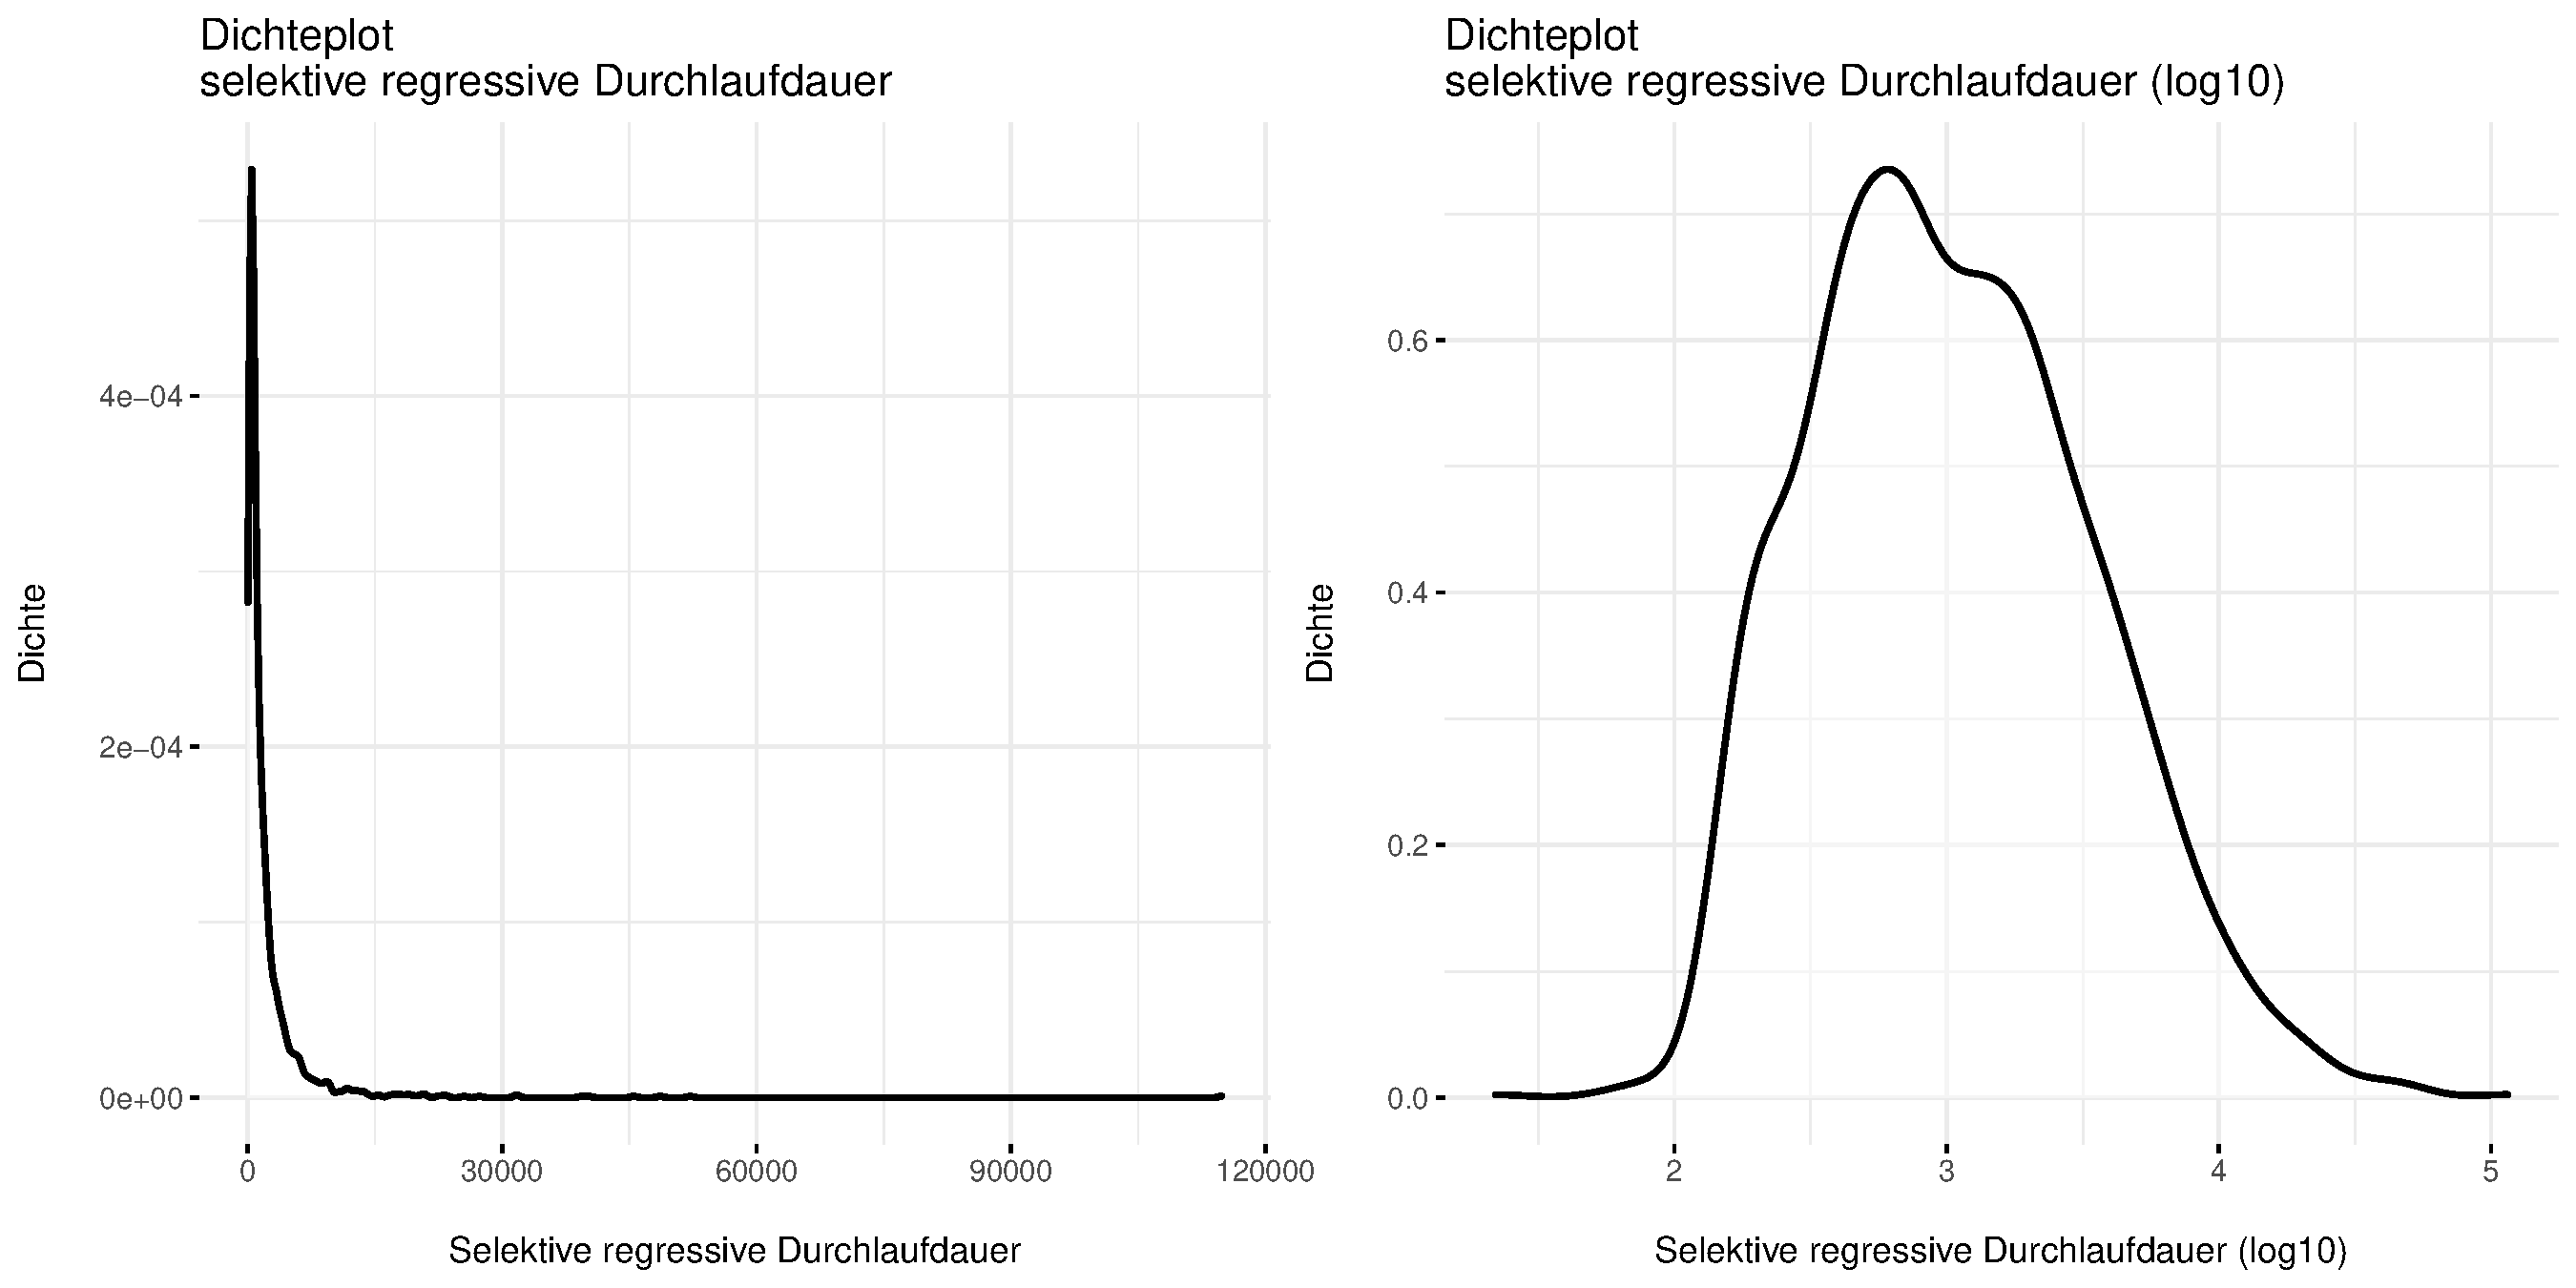
\includegraphics[width=\textwidth]{Figures/EyeTracking/CatDe/ggplot_catde-select-RegPD_density_de}}
	\caption{Verteilung selektive regressive Durchlaufdauer: normal (links), logarithmisch transformiert (rechts)}
	\label{K6:fig:CatDe:density-iaselregpd}
\end{figure}
\vfill\pagebreak

%------------------------------------

Die selektive regressive Durchlaufdauer korreliert signifikant\is{Spearman's Rho}\is{Korrelationstest nach Spearman}\is{Statistik!Testverfahren!Korrelationstest nach Spearman} mit der Größe der AOI ($r_{s} = 0,34, p < 0,01, n = 482.868.254$). Dabei handelt es sich nach \citet{cohen_power_1992} um einen schwachen Effekt. Das Bestimmtheitsmaß beträgt 11,45\,\%.\is{Durchlauf!-dauer!selektive regressive|)}


%------------------------------------------------------------------------

\subsubsection{Pupillengröße}
\label{K6:subsubsec:psize:catde}

%------------------------------------------------------------------------

\is{Pupillengröße|(}
\tabref{K6:tab:CatDe:mean-sd-psize} zeigt die Mittelwert und Standardabweichung der Pupillengröße in willkürlichen Einheiten pro AOI-Kategorie. Im katalanisch-deutschen Versuchsaufbau liegt die durchschnittliche Pupillengröße bei Betrachtung der Eingabemaske 92 Einheiten über dem Gesamtschnitt. Das entspricht einer Pupillenweitung um 17\,\%. Dies kann mitunter daran liegen, dass die Proband{\textperiodcentered}innen den Bereich der Eingabe nutzen, um auf eingehende Nachrichten zu warten. Besonders dem Symbol \glqq Schreibt gerade\dots\grqq{} kommt dabei eine zentrale Rolle zu, wie \citet[]{schlosser_beyond_2018} in seinem Beitrag aufgreift. Dieses Symbol wird als zentraler Fokuspunkt auch im Angesicht der Rollenorganisation\is{Rollenorganisation|see{Sprecher{\textperiodcentered}innenorganisation}} der Chatter{\textperiodcentered}innen genutzt, um die Augen ruhen zu lassen und im Folgenden auf die Antwort des Gegenübers zu warten. Das Erfassen der Chatbeiträge des Gegenübers in der Muttersprache erhöht die kognitive Auslastung hingegen nicht signifikant, wie eine Testwiederholung unter Vernachlässigung der Eingabemaske belegen.

%------------------------------------



\begin{table}
   \begin{tabular}{lccc}  
    \lsptoprule
        {AOI-Kategorie} & {Mittelwert} & {Median} & {SD} \\ 
        \midrule
        GerO  & 505,39 & 504,40 & 82,84 \\ 
        CatMT &  558,21 & 564,07 & 86,11 \\ 
        CatO &  538,32 & 541,75 & 92,57 \\ 
        GerMT &  546,93 & 554,83 & 87,66 \\ 
        Eingabe &  632,93 & 640,69 & 61,44 \\ 
        \midrule
        Global  & 540,55 & 545,48 & 89,78 \\ 
        \lspbottomrule
    \end{tabular}
        \caption[Mittelwert, Median und SD der Pupillengröße (AOI)]{Mittelwert, Median und SD der Pupillengröße pro AOI-Kategorie in willkürlichen Einheiten}
    \label{K6:tab:CatDe:mean-sd-psize}
\end{table}

%------------------------------------

Im Setting Katalanisch-Deutsch sind es die Vergleichsgruppen mit Beteiligung der jeweiligen MÜ-Ausgabe, die signifikante Unterschiede in der Pupillengröße aufweisen. Die Pupillenweitung der MÜ-Ausgabe ins Deutsche liegt 1\,\% (\emph{GerMT}: 546 Einheiten, Durchschnitt 540 Einheiten) über dem Durchschnitt. Die Pupillengröße beim deutschen Originalbeitrag ist 7\,\% kleiner als der Durchschnitt (\emph{GerO}: 505 Einheiten, Durchschnitt: 540 Einheiten). Der Unterschied zwischen beiden Gruppen beträgt 8\,\%.

Wie auch die MÜ-Ausgabe ins Deutsche liegt die Pupillengröße des katalanischen Originals nah am globalen Schnitt (\emph{GerMT}: 546 Einheiten, \emph{CatO}: 538 Einheiten, Unterschied 0,4\,\%). Die MÜ-Ausgabe ins Katalanische liegt 3\,\% über dem Schnitt (558 Einheiten). Der Unterschied zwischen beiden Kategorien beträgt 3,5\,\%. Die statistisch signifikanten Unterschiede der Pupillengröße beider katalanischen Kategorien könnte auf Priming-Effekte zurückzuführen sein. Diese Vermutung drängt sich durch die statistische Betrachtung der progressiven ersten Fixation auf. Die Pupillengröße unterscheidet sich zwischen AOI, die vorab bersprungen wurden, und solchen, die regulär in chronologischer Reihenfolge betrachtet wurden. Die Möglichkeit einer aufgabeninternen Varianz der Pupillengröße wurde hingegen nicht untersucht. \citet[6\psq]{hyona_pupil_1995} beschreiben in ihrer Studie die Veränderungen der Pupillengröße der Proband{\textperiodcentered}innen über die gestellte Aufgabe hinweg und stellen dabei signifikante Unterschiede fest, deren Ursprung sie in einem Gewöhnungsprozess verorten.

%------------------------------------------------------------------------

\begin{figure}
	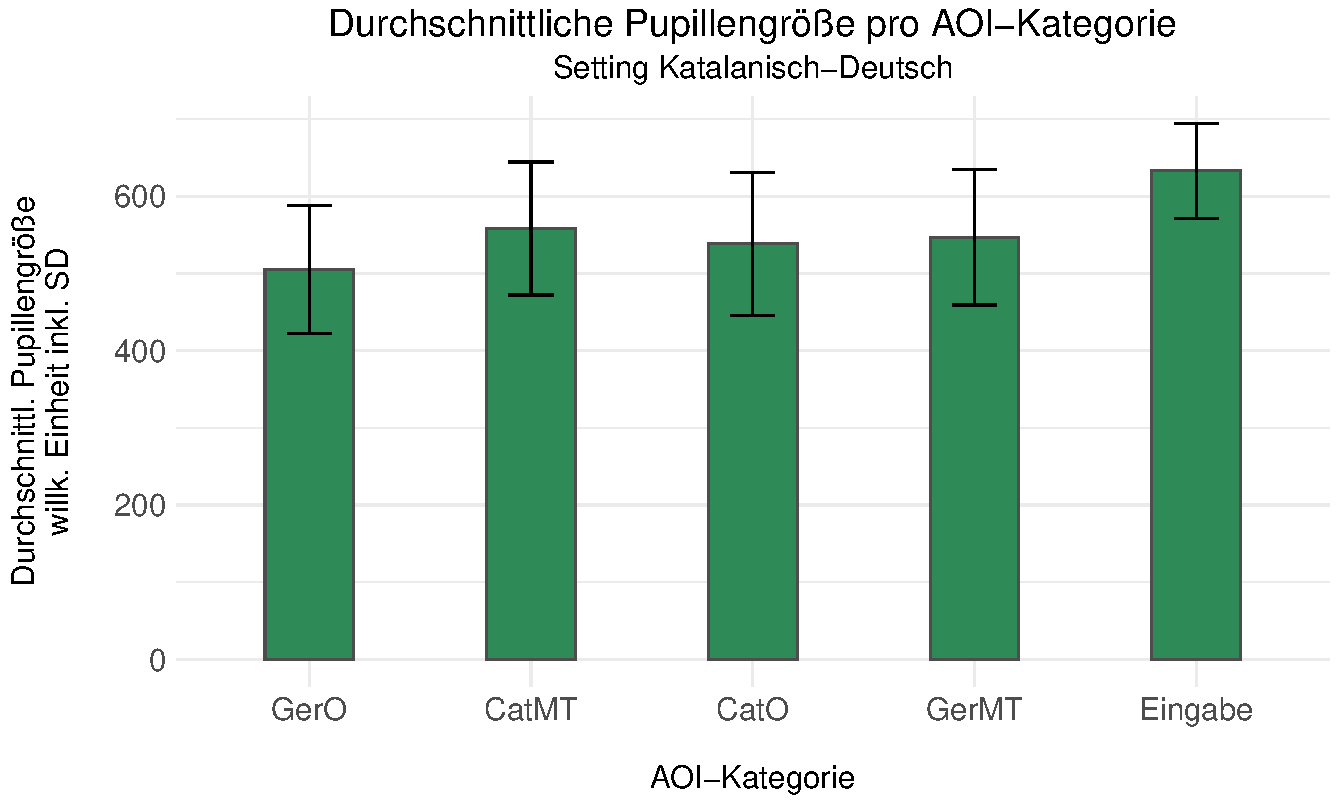
\includegraphics[width=.85\textwidth]{Figures/EyeTracking/CatDe/ggplot_catde_meanPSize_de}
	\caption{Durchschnittliche Pupillengröße pro AOI-Kategorie im Setting Katalanisch-Deutsch}
	\label{K6:fig:CatDe:mean-error-psize}
\end{figure}

%------------------------------------------------------------------------


%------------------------------------------------------------------------

\begin{figure}
	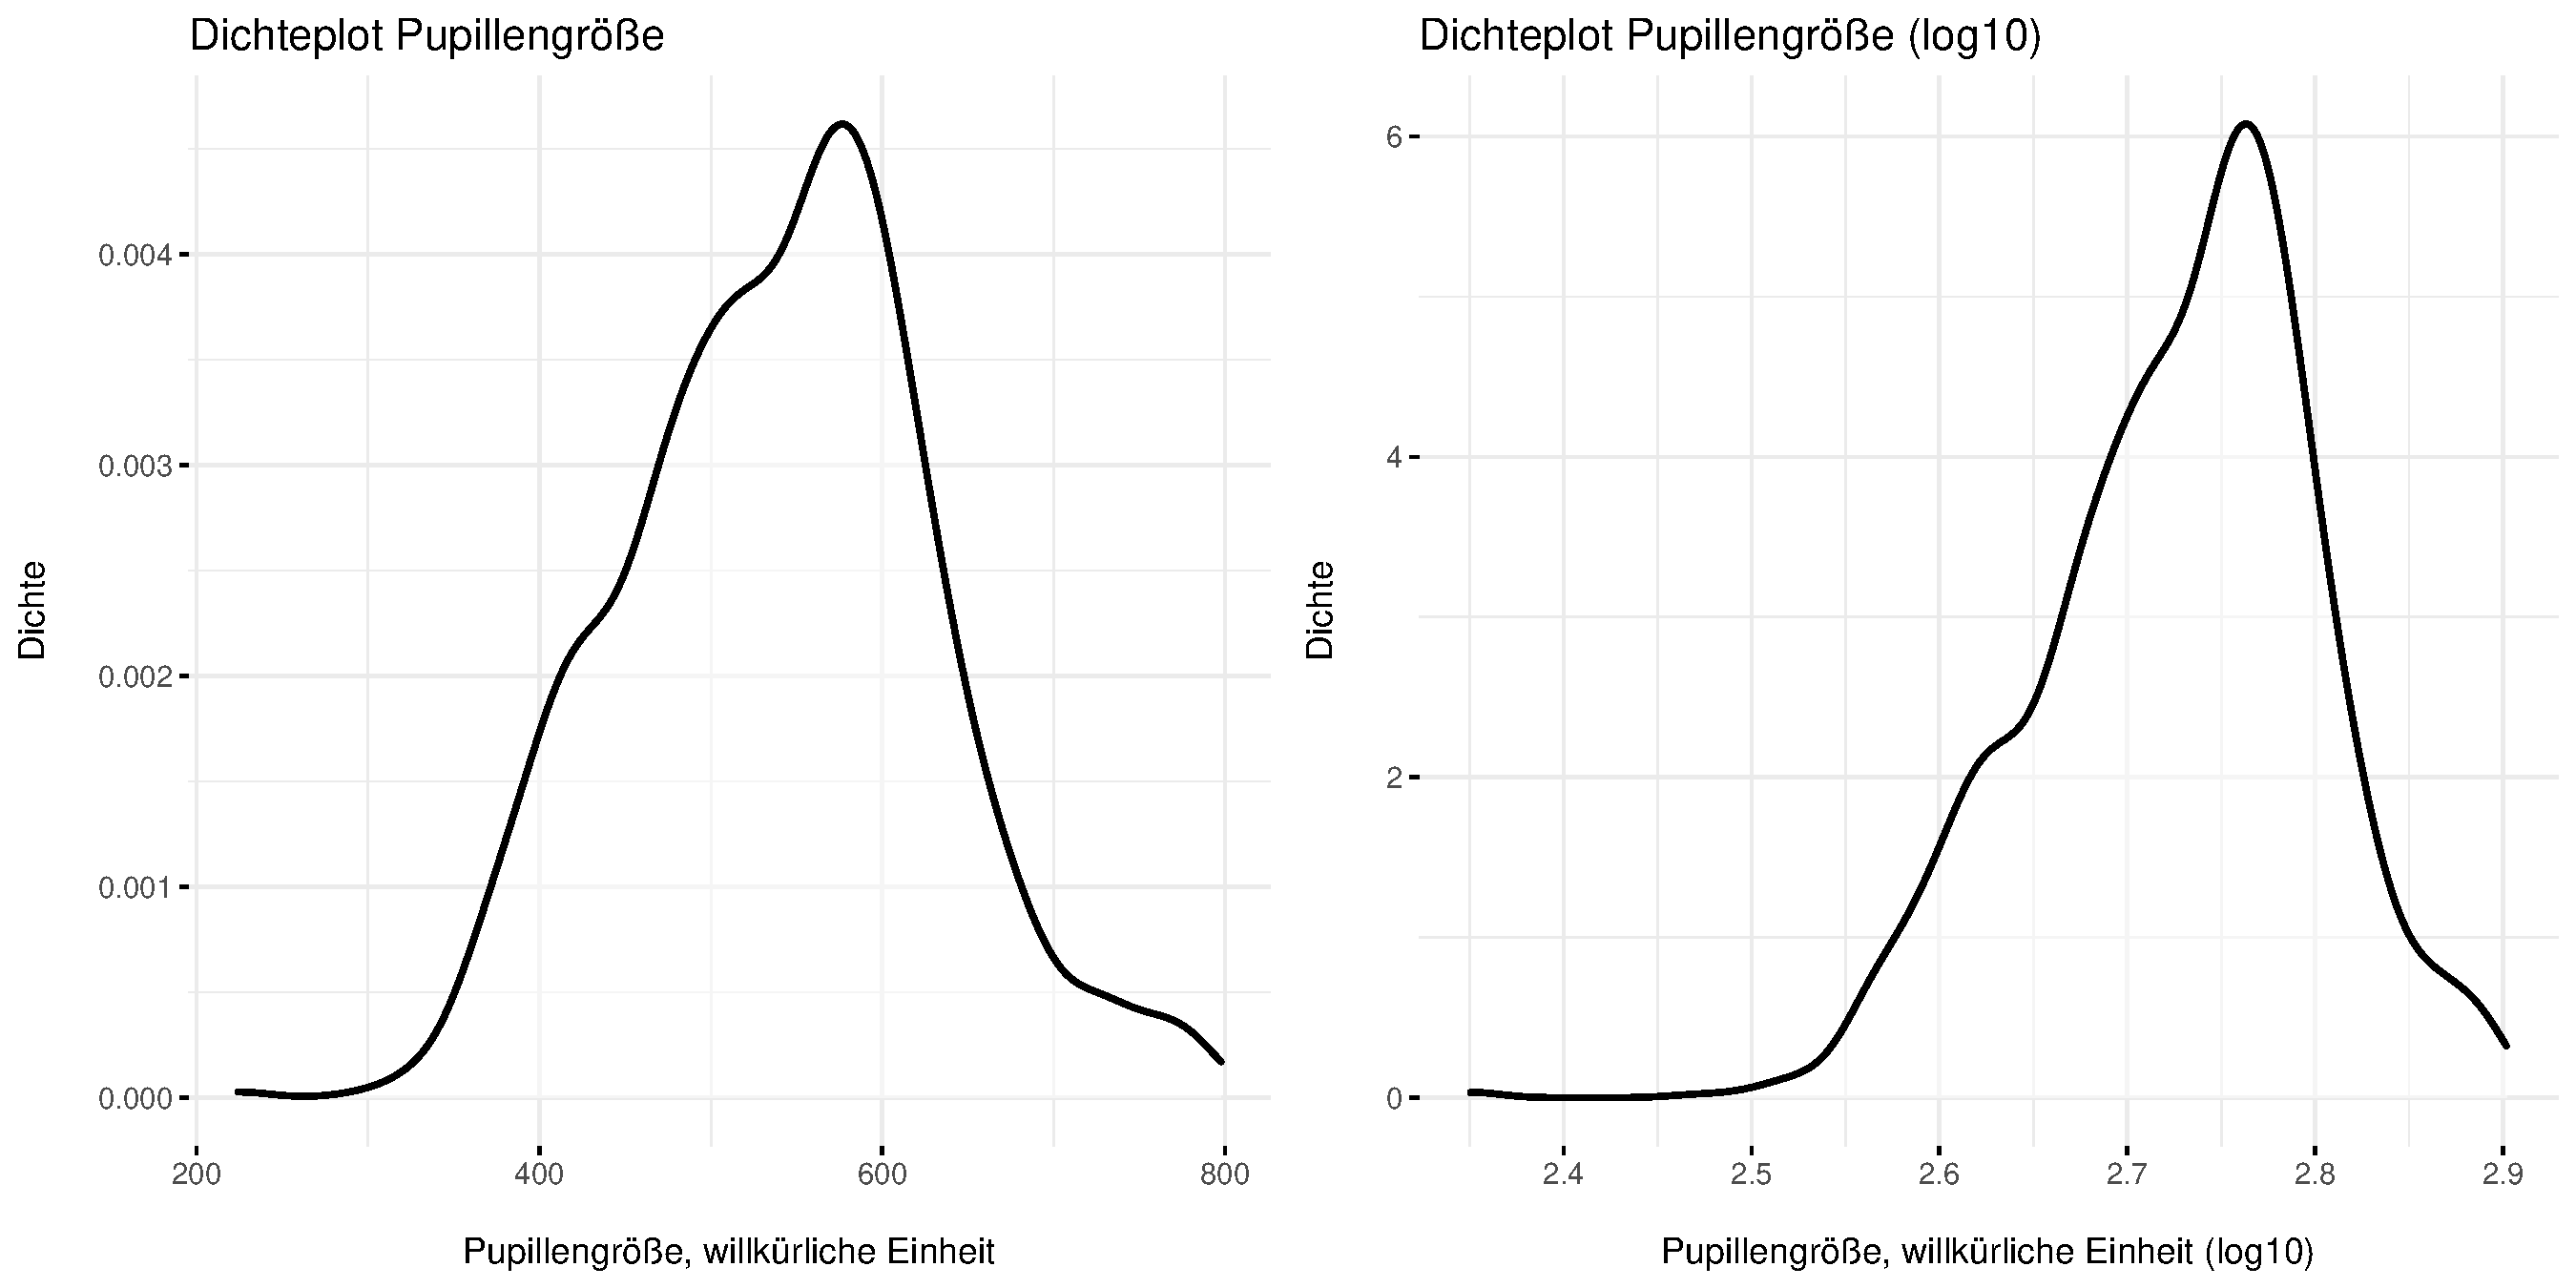
\includegraphics[width=\textwidth]{Figures/EyeTracking/CatDe/ggplot_catde-PSize_density_de}
	\caption{Verteilung der Pupillengröße in willkürlichen Einheiten: normal (links), logarithmisch transformiert (rechts)}
	\label{K6:fig:CatDe:density-PSize}
\end{figure}

%------------------------------------------------------------------------

Eine graphische Inspektion der Daten (\figref{K6:fig:CatDe:density-PSize}) zeigt, dass weder die rohen noch die logarithmisch transformierten\is{Statistik!Transformation!logarithmische} Werte normalverteilt sind. Auch die statistische Untersuchung unter Anwendung des Shapiro-Wilk-Tests\is{Statistik!Testverfahren!Shapiro-Wilk-Test} deutet auf nicht normalverteilte Daten hin (roh: $W = 0,99, p < 0,001$, log10: $W = 0,98,\allowbreak\ p < 0,001$). Daher wird die Pupillengröße mit nicht-parametrischen Tests untersucht.

Ein Kruskal-Wallis-Test\is{Statistik!Testverfahren!Kruskal-Wallis-Test} deutet darauf hin, dass Unterschiede in der zentralen Tendenz der Pupillengröße pro AOI zwischen den einzelnen Teilnehmer{\textperiodcentered}innen bestehen ($\chi^2(20) = 937,34, p < 0,01$). Anschließend durchgeführte Post-hoc-Tests (Dunn-Benjamini-Hochberg-Tests)\is{Statistik!Testverfahren!Dunn-Benjamini-Hochberg-Test} zeigen, dass sich 168 von möglichen 210 TN-Paaren (80,00\,\%) signifikant unterscheiden, sodass gefolgert werden kann, dass Unterschiede bei der Pupillengröße in gewissem Maße zwischen den einzelnen Teilnehmer{\textperiodcentered}innen bestehen. Auch eine Betrachtung der Mittelwerte (s. \tabref{K6:tab:CatDe:mean-sd-psize-TN}) spiegelt diese Einschätzung wieder. Der globale Mittelwert liegt bei 540 Einheiten, wobei die mittlere Pupillengröße je nach Teilnehmer{\textperiodcentered}in z.\,T.\ stark variiert.

%------------------------------------


	
\begin{table}
    \begin{tabular}{lS[table-format=3.2]cc} 
    \lsptoprule
        {Pseudonym} & {Mittelwert} & {Median}  & {SD} \\ 
        \midrule
        TN11  & 603,98 & 598,97 & 46,39 \\ 
     TN12  & 584,90 & 578,72 &  47,62 \\ 
      TN13  & 525,92 &518,33 & 65,68 \\ 
      TN15   &410,26 &408,36 & 54,73 \\ 
      TN16   &606,55 & 605,77 & 44,83 \\ 
      TN17   &585,97 & 579,85 & 35,93 \\ 
      TN18   &562,73 & 560,76 & 62,05 \\ 
     TN19   &532,11 &524,69 & 54,24 \\ 
      TN20  & 436,40 & 423,45 &  60,03 \\ 
     TN21   &527,19 & 522,46 & 93,08 \\ 
     TN22   &620,27 & 627,38 & 79,71 \\ 
     TN23   &703,58 & 717,50 & 53,66 \\ 
     TN24   &532,53 & 512,00 & 83,71 \\ 
     TN25   &592,96 &594,67 & 51,06 \\ 
      TN3   &530,05 & 508,73 & 66,04 \\ 
      TN4   &498,15 & 494,65 & 41,11 \\ 
      TN5   &497,9 & 493,79 & 44,54 \\ 
      TN6  & 536,84 & 542,65 & 48,96 \\ 
      TN7 &  516,52 & 501,47 & 80,53 \\ 
      TN8  & 436,98 & 425,40 & 48,88 \\ 
      TN9  & 555,49 & 563,85 & 58,12 \\ 
      \midrule
   Global  & 540,55 &545,48 & 89,78 \\ 
   \lspbottomrule
    \end{tabular}
        \caption[Mittelwert, Median und SD der Pupillengröße (TN)]
                {Mittelwert, Median und SD der Pupillengröße pro Studienteilnehmer{\textperiodcentered}in\label{K6:tab:CatDe:mean-sd-psize-TN}}
\end{table}

%------------------------------------


Ein weiterer Kruskal-Wallis-Test\is{Statistik!Testverfahren!Shapiro-Wilk-Test} ergibt, dass Unterschiede bei der Pupillengröße zwischen den einzelnen AOI-Kategorien bestehen ($\chi^2(4) = 91,45, p < 0,01$). Anschließend durchgeführte Post-hoc-Tests (Dunn-Benjamini-Hoch\-berg-Tests, s. \tabref{K6:tab:CatDe:dunntest-pupilsize})\is{Statistik!Testverfahren!Dunn-Benjamini-Hochberg-Test} zeigen, dass sich 8/10 Gruppierungen unterscheiden, sodass gefolgert werden kann, dass die Pupillengröße von der AOI-Kategorie abhängt. Die Gruppierungen \emph{CatO--GerMT} sowie \emph{CatMT--GerMT} unterscheiden sich hingegen nicht signifikant. Die kognitive Auslastung bei der Betrachtung der MÜ ins Deutsche ist demnach vergleichbar mit der bei der Erfassung der katalanischsprachigen Nachrichten.

%------------------------------------

\begin{table}
    \begin{tabular}{lS[table-format=-1.6]S[table-format=1.4]@{ }lS[table-format=1.2]}  
    \lsptoprule
        {AOI-Kategoriepaar} & {$z$} & \multicolumn{2}{c}{$p$ (angepasst)} & {Effekt}\\ 
        \midrule
        CatMT-CatO    &  3,135705 & 0,0011 & ** & 0,11 \\ 
        CatMT-Eingabe & -3,934707 & 0,0001 & *** & 0,2 \\ 
        CatO-Eingabe  & -4,929169 & 0,0000 & *** & 0,23 \\ 
        CatMT-GerMT   &  1,730853 & 0,0464 & & \\ 
        CatO-GerMT    & -1,592935 & 0,0556 & & \\ 
        Eingabe-GerMT &  4,487021 & 0,0000 & *** & 0,2\\ 
        CatMT-GerO    &  7,743269 & 0,0000 & *** & 0,30\\ 
        CatO-GerO     &  5,061620 & 0,0000 & *** & 0,19\\ 
        Eingabe-GerO  &  6,533117 & 0,0000 & *** & 0,37\\ 
        GerMT-GerO    &  6,659042 & 0,0000 & *** & 0,23\\ 
        \lspbottomrule
    \end{tabular}
    \caption{Ergebnisse des Dunn-Tests: Gruppierte Vergleiche der Pupillengröße nach AOI-Kategorie\label{K6:tab:CatDe:dunntest-pupilsize}}
\end{table}


%------------------------------------
\largerpage[-1]
Mit einer weiteren Testfolge sollen die Unterschiede zwischen progressiver erstmaliger Fixation\is{Fixation!progressive erste} und der Pupillengröße untersucht werden. Da diese Fixationsart nur in zwei Ausprägungen vorliegt (0 und 1), wird nicht der Kruskal-Wallis-Test, sondern der Mann-Whitney-U-Test\is{Statistik!Testverfahren!Mann-Whitney-U-Test} verwendet. In Bezug auf den globalen Datensatz ($U = 370.818,0, p < 0,001$) besteht ein signifikanter Unterschied in der zentralen Tendenz der Pupillengröße zwischen den AOI, die von einem AOI mit höherer Ordnungszahl heraus betreten wurden, und denen, die chronologisch betrachtet wurden. Wie hierzu aus \tabref{K6:tab:CatDe:mwutest-pupilsize-ffixpro} ersichtlich wird, beeinflusst die progressive erste Fixation\is{Fixation!progressive erste} auch pro AOI-Kategorie die Pupillengröße signifikant.

%------------------------------------


\begin{table}
    \begin{tabular}{lrS[table-format=1.4]@{ }lS[table-format=1.2]}  
    \lsptoprule
        {AOI-Kategorie} & \multicolumn{1}{c}{$U$} & \multicolumn{2}{c}{$p$ (angepasst)} & {Effekt}\\\midrule
        GerO    &  21.301,5 & 0,016 &* & 0,14 \\ 
        CatMT  & 9.557,5 & 0,0001& *** & 0,23\\ 
        CatO  & 46.275,5 & 0,0001& *** & 0,14 \\ 
        GerMT   &  18.324,0  & 0,0001 & *** & 0,21 \\ 
        Eingabe & 25,0 & 0,614 &   \\
        \midrule
        Global & 370.818,0 & 0,001 & ** & 0,22 \\ 
        \lspbottomrule
    \end{tabular}
        \caption[Ergebnisse des Mann-Whitney-U-Tests zur Pupillengröße]{Ergebnisse des Mann-Whitney-U-Tests zur Pupillengröße und progressiven ersten Fixation nach AOI-Kategorie}
    \label{K6:tab:CatDe:mwutest-pupilsize-ffixpro}
\end{table}


%------------------------------------

Die Pupillengröße korreliert zudem signifikant mit der Größe der AOI ($r_{s} = -0,20, p < 0,01, n = 839.458.138$)\is{Spearman's Rho}\is{Korrelationstest nach Spearman}\is{Statistik!Testverfahren!Korrelationstest nach Spearman}. Dabei handelt es sich nach \citet{cohen_power_1992}\is{Effektstärke nach Cohen}\is{Statistik!Testverfahren!Effektstärke nach Cohen} um einen schwachen Effekt. Das Bestimmtheitsmaß beträgt 3,83\,\%.
\is{Pupillengröße|)}


%------------------------------------------------------------------------

\subsection{Das sakkadische Blickverhalten}
\label{K6:subsec:sacGaze-CatDe}

%------------------------------------------------------------------------

\is{Sakkade!Anzahl an|(}
Tabelle \ref{K6:tab:CatDe:sacspecs} stellt die absolute Anzahl an Sakkaden pro AOI im Setting Ka\-ta\-la\-nisch-Deutsch dar. Beinahe drei Mal so viele Sakkaden werden innerhalb der MÜ-Ausgabe ins Deutsche getätigt wie im deutschen Original. Die wenigsten Sakkaden werden in den ausgehenden Beiträgen der Proband{\textperiodcentered}innen getätigt, hier ist der Wert sogar noch niedriger als im AOI der Eingabemaske. Auf das katalanische Original entfallen weniger als halb so viele Sakkaden (2.198) wie auf die MÜ ins Deutsche (2.405). Ähnlich weit auseinander liegt die Anzahl an Sakkaden beim deutschen Original (1.835) und der MÜ ins Katalanische (3.229). Die entsprechenden Mittelwerte betragen für das deutsche Original 5,65, für die MÜ ins Katalanische 8,36, für das katalanische Original 11,98 und für die MÜ ins Deutsche 13,23. Im Durchschnitt werden also mehr Sakkaden innerhalb des katalanischen Originals und der MÜ ins Deutsche getätigt als im deutschen Original und der MÜ ins Katalanische. Pro AOI werden im gesamten Datensatz im Schnitt 55,30 Sakkaden erfasst. Die Standardabweichung ist mit Blick auf den gesamten Datensatz außergewöhnlich hoch. Es kann daher von einer starken Varianz innerhalb des Satzes ausgegangen werden. Da die Eingabemaske als statisches AOI annotiert wurde, ist eine Berechnung der durchschnittlichen Sakkadenanzahl nicht möglich.

%------------------------------------


	
\begin{table}
    \begin{tabular}{lrS[table-format=2.2]r} 
    \lsptoprule
        {AOI-Kategorie} & \multicolumn{1}{c}{Anzahl} & {Mittelwert} & \multicolumn{1}{c}{SD} \\
        \midrule
        GerO  & 1.835 & 9 & 5,65 \\ 
        CatMT  & 3.229 & 8,36 & 6,15\\ 
        CatO   & 2.198 & 11,98 & 8,03\\ 
        GerMT  & 5.320 & 13,23 & 8,96\\ 
        Eingabe  & 2.405 &  & \\ \midrule
        Global & 14.987 & 55,30 & 7.108,98\\ 
        \lspbottomrule
    \end{tabular}
        \caption{Anzahl, Mittelwert und SD der Sakkaden pro AOI-Kategorie}
    \label{K6:tab:CatDe:sacspecs}
\end{table}


%------------------------------------

%------------------------------------------------------------------------

%%%% Multi-Table: 3x2, wobei nur 2x2x1 Kacheln belegt sind mit den jeweiligen Kategorien GerO, GerMT, CatO, CatMT, Eingabe

\begin{table}
    \begin{minipage}{0.5\textwidth}\centering
        \begin{tabular}{lrr} 
        \lsptoprule
         Kategorie & \multicolumn{2}{c}{{GerO}} \\ 
         \cmidrule(lr){2-3}
            {Richtung} & \multicolumn{1}{c}{Anzahl} & \multicolumn{1}{c}{Prozent} \\ 
            \midrule
            Runter & 26 & 1,42 \\ 
            Links & 410 & 22,34 \\ 
            Rechts & 1.284 & 69,87 \\ 
            Hoch & 104 & 5,67 \\ 
            \emph{NA} & 11 & 0,60 \\ 
            \midrule
            {Gesamt} & 1.835 & 100 \\ 
            \lspbottomrule
            \end{tabular}
            \end{minipage}\begin{minipage}{0.5\textwidth}\centering
             \begin{tabular}{lrr} 
             \lsptoprule
             Kategorie & \multicolumn{2}{c}{{CatMT}} \\ 
             \cmidrule(lr){2-3}
            {Richtung} & \multicolumn{1}{c}{Anzahl} & \multicolumn{1}{c}{Prozent}  \\ 
            \midrule
            Runter & 150 & 4,65 \\ 
            Links & 811 & 25,12 \\ 
            Rechts & 1.876 & 58,10 \\ 
            Hoch & 362 & 11,21 \\ 
            \emph{NA} & 30 & 0,93 \\ 
            \midrule
            {Gesamt} & 3.229 & 100 \\ 
            \lspbottomrule
         \end{tabular}    
    \end{minipage}\medskip\\
    \begin{minipage}{0.5\textwidth}\centering
             \begin{tabular}{lrr} 
             \lsptoprule
             Kategorie & \multicolumn{2}{c}{{CatO}} \\ 
             \cmidrule(lr){2-3}
            {Richtung} & \multicolumn{1}{c}{Anzahl} & \multicolumn{1}{c}{Prozent}  \\ 
            \midrule
            Runter & 122 & 5,55 \\ 
            Links & 541 & 24,61 \\ 
            Rechts & 1.124 & 51,14 \\ 
            Hoch & 395 & 17,97 \\ 
            \emph{NA} & 16 & 0,73 \\ 
            \midrule
            {Gesamt} & 2.198 & 100 \\ 
            \lspbottomrule
         \end{tabular}    
    \end{minipage}\begin{minipage}{0.5\textwidth}\centering
             \begin{tabular}{lrr} 
             \lsptoprule
             Kategorie & \multicolumn{2}{c}{{GerMT}} \\ 
             \cmidrule(lr){2-3}
            {Richtung} & \multicolumn{1}{c}{Anzahl} & \multicolumn{1}{c}{Prozent}  \\ 
            \midrule
            Runter & 327 & 6,15 \\ 
            Links & 1.164 & 21,88 \\ 
            Rechts & 3.345 & 62,88 \\ 
            Hoch & 457 & 8,59 \\ 
            \emph{NA} & 27 & 0,51 \\ 
            \midrule
            {Gesamt} & 5.320 & 100 \\ 
            \lspbottomrule
         \end{tabular}    
    \end{minipage}\medskip\\\begin{minipage}{0.5\textwidth}\centering
             \begin{tabular}{lrr}
             \lsptoprule
             Kategorie & \multicolumn{2}{c}{{Eingabe}} \\ 
             \cmidrule(lr){2-3}
            {Richtung} & \multicolumn{1}{c}{Anzahl} & \multicolumn{1}{c}{Prozent}  \\ 
            \midrule
            Runter & 414 & 17,21 \\ 
            Links & 797 & 33,14 \\ 
            Rechts & 1.052 & 43,74 \\ 
            Hoch & 107 & 4,45 \\ 
            \emph{NA} & 35 & 1,46 \\ 
            \midrule
            {Gesamt} & 2.405 & 100 \\ 
            \lspbottomrule
         \end{tabular}    
    \end{minipage}
     \caption{Sakkadenanzahl nach Richtung und AOI-Kategorie im Setting Katalanisch-Deutsch}
    \label{K6:tab:saccount-direction-CatDe}
\end{table}


%------------------------------------------------------------------------

\is{Sakkade!gerichtete|(}
\begin{sloppypar}
\tabref{K6:tab:saccount-direction-CatDe} zeigt die aufsummierte Sakkadenanzahl nach AOI und Richtung im Versuchssetting Katalanisch-Deutsch. Sakkaden, die außerhalb eines AOI gelandet sind, werden unter \emph{NA} gezählt. Innerhalb aller AOI-Kategorien dominieren nach rechts gerichtete Sakkaden. In allen Kategorien beträgt der Anteil jeweils über 50\,\% mit Ausnahme der Eingabemaske. Der Anteil rechtsgerichteter Sakkaden ist im Vergleich zu den linksgerichteten Sakkaden auffällig gering. Die linksgerichteten Sakkaden in den übrigen vier Kategorien machen jeweils einen Anteil von 20--25\,\% aus. Auffälliger sind die unterschiedlich hohen Anteile an nach oben gerichteten Sakkaden. Im Falle des deutschen Originals und der MÜ ins Deutsche liegen die Anteile jeweils unter 10\,\%, bei der MÜ ins Katalanische bei etwas mehr als 11\,\% und beim katalanischen Original erreicht der Anteil sogar beinahe 18\,\%. 
\end{sloppypar}
\is{Sakkade!gerichtete|)}
\is{Sakkade!Anzahl an|)}


%------------------------------------------------------------------------

\subsubsection{Sakkadenamplitude}
\label{K6:subsubsec:sacamp:catde}

%------------------------------------------------------------------------

\is{Sakkade!-namplitude|(}
Im Gegensatz zur statistischen Untersuchung der Normalverteilung der fixatorischen Indikatoren mit dem Shapiro-Wilk-Test wurde die Verteilung der Sakkadendaten mit dem Anderson-Darling-Test betrachtet. Dieser Test kann größere Datensätz erfassen als der Shapiro-Wilk-Test. 
Der Anderson-Darling-Test\is{Anderson-Darling-Test|see{Statistik}}\is{Statistik!Testverfahren!Anderson-Darling-Test}\is{Anderson-Darling-Test} belegt, dass sowohl die Gesamtheit des Datensatzes als auch der Datensatz nach einzelnen AOI-Kategorien in Bezug auf die Sakkadenamplitude nicht normalverteilt ist. Es ergibt sich für die Gesamtheit ein Verteilungswert im AD-Test von ($A = 1.253,1, p < 0,01$) und für die Kategorien \emph{GerO}: ($A = 162,84, p < 0,01$), \emph{CatMT}: ($A = 305,34, p < 0,01$), \emph{CatO}: ($A = 168,12, p < 0,01$), \emph{GerMT}: ($A = 393,26,\allowbreak\ p < 0,01$) und Eingabe: ($A = 226,42, p < 0,01$). Auch eine logarithmische Transformation\is{Statistik!Transformation!logarithmische} änderte die Verteilung nicht wesentlich (s. \figref{K6:fig:CatDe:sacamp-density}). Auf die Kategorie \emph{GerO} verfallen so noch 1.835 Sakkaden, 3.229 auf \emph{CatMT}, 2.198 auf \emph{CatO}, 5.320 auf \emph{GerMT} und 2.405 auf die Eingabemaske. Insgesamt enthält der Datensatz somit noch 14.987 Sakkaden.

Es besteht eine lineare Abhängigkeit zwischen Sakkadenamplitude und -dauer, was \citet[321]{holmqvist_eye_2011} mit Verweis auf \citet[]{carpenter_movements_1988} herausstellt. Die genaue Art der Abhängigkeit kann mittels eines Korrelationstests mit Spearman's Rho\is{Spearman's Rho}\is{Korrelationstest nach Spearman}\is{Statistik!Testverfahren!Korrelationstest nach Spearman} untersucht werden. Sowohl der gesamte Datensatz als auch die Werte nach einzelnen AOI-Kategorien getrennt stehen demnach signifikant in einer positiven Beziehung zueinander: Gesamt: ($S = \num{2.9267e11}, p < 0,01, r = 0,65$), \emph{GerO}: ($S = 368.854.171, p < 0,01, r = 0,76$), \emph{CatMT}: ($S = 3.028.797.579,\allowbreak\ p < 0,01,\allowbreak r = 0,64$), \emph{CatO}: ($S = 784.453.871, p < 0,01, r = 0,7$), \emph{GerMT}: ($S = \num{1.0672e10},\allowbreak\ p < 0,01, r = 0,69$) und Eingabe: ($S = 2.144.558.389, p < 0,01, r = 0,46$).\largerpage[2]

%------------------------------------


\begin{table}
    \begin{tabular}{lccc}
    \lsptoprule
        {AOI-Kategorie} & {Mittelwert} & {Median} & {SD} \\ 
        \midrule
        GerO  & 1,94 & 1,42 & 1,51\\ 
        CatMT  & 1,82 & 1,29 & 1,47\\ 
        CatO   & 1,90 & 1,42 & 1,42\\ 
        GerMT  & 1,79 & 1,37 & 1,30\\ 
        Eingabe  & 1,86 & 1,29 & 1,56\\ 
        \midrule
        Global & 1,84 & 1,35 & 1,43\\ 
        \lspbottomrule
    \end{tabular}
        \caption[Mittelwert, Median und SD der Sakkadenamplitude]{Mittelwert, Median und SD der Sakkadenamplitude pro AOI-Kategorie}
    \label{K6:tab:CatDe:sacamp}
\end{table}


%------------------------------------


%------------------------------------------------------------------------

\begin{figure}
    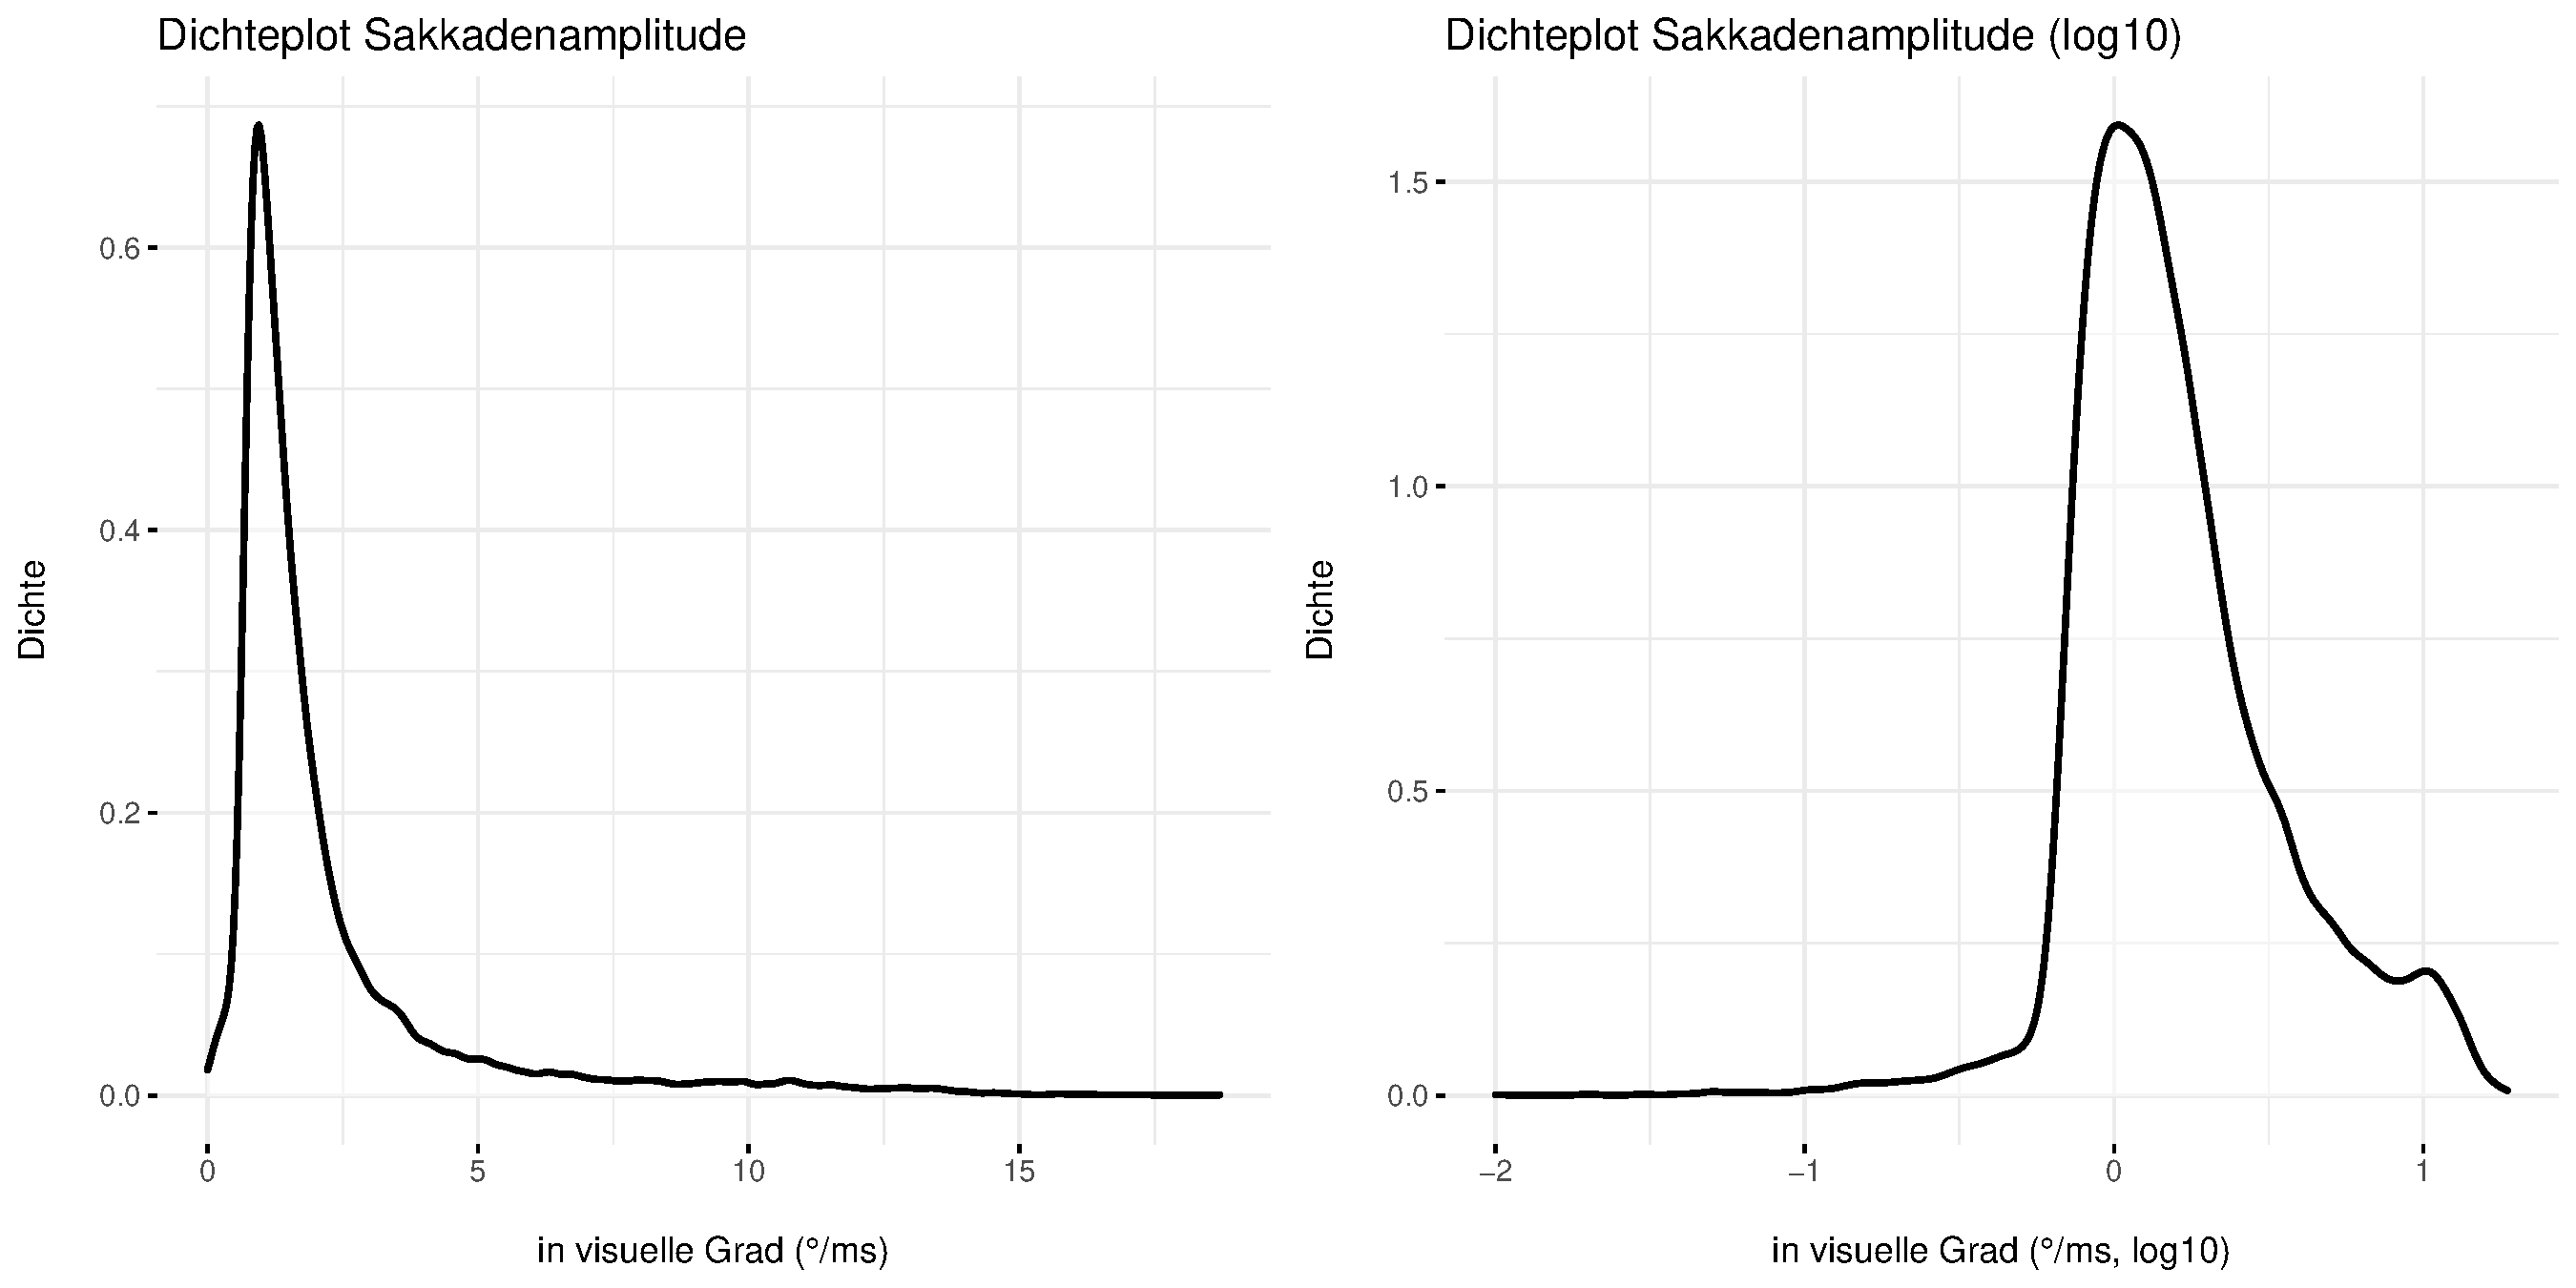
\includegraphics[width=\textwidth]{Figures/EyeTracking/CatDe/ggplot_CatDe-SacAmp_density_de}
	\caption{Verteilung der Sakkadenamplitude: normal (links), logarithmisch transformiert (rechts)}
	\label{K6:fig:CatDe:sacamp-density}
\end{figure}

%------------------------------------------------------------------------

Ein Kruskal-Wallis-Test\is{Statistik!Testverfahren!Kruskal-Wallis-Test} deutet darauf hin, dass Unterschiede in der zentralen Tendenz der Sakkadenamplitude zwischen den einzelnen Teilnehmer{\textperiodcentered}innen bestehen ($\chi^2(20) = 286,86, p < 0,01$). Anschließend durchgeführte Post-hoc-Tests (Dunn-Benjamini-Hochberg-Tests)\is{Statistik!Testverfahren!Dunn-Benjamini-Hochberg-Test} zeigen, dass sich 134 von 210 möglichen Gruppierungen (63,81\,\%) signifikant voneinander unterscheiden, sodass gefolgert werden kann, dass die Sakkadenamplitude in gewissem Maße von der Individualität der TN abhängt. Dies ist nicht weiter verwunderlich, da \citet[312]{holmqvist_eye_2011} betont, dass die Sakkadenamplitude starken Variationen pro Teilnehmer{\textperiodcentered}in unterliegt.

\begin{sloppypar}
Ein zweiter Kruskal-Wallis-Test\is{Statistik!Testverfahren!Kruskal-Wallis-Test} zeigt weiterhin, dass Unterschiede in der Sakkadenamplitude zwischen den einzelnen AOI-Kategorien bestehen ($\chi^2(4) = 56,56,\allowbreak\ p < 0,01$). Anschließend durchgeführte Post-hoc-Tests (Dunn-Benjamini-Hochberg-Tests)\is{Statistik!Testverfahren!Dunn-Benjamini-Hochberg-Test} zeigen, dass sich 8 von 10 möglichen Gruppierungen unterscheiden, sodass gefolgert werden kann, dass die Sakkadenamplitude von der betrachteten AOI-Kategorie beeinflusst wird (s. \tabref{tab:CatDe:dunntest-sacamp}, der Asterisk zeigt das Signifikanzlevel an: * $\alpha < 0,05$). Die Ausnahme bilden die Paare \emph{CatMT-Eingabe} sowie \emph{CatO-GerO}. Eine Effektstärke nach \citet{cohen_power_1992} ist hier jedoch nicht nachweisbar ($r < 0,1$).\end{sloppypar}


%------------------------------------

\begin{table}
    \begin{tabular}{lS[table-format=-1.6]S[table-format=1.4]@{ }lr}  
    \lsptoprule
        {AOI-Kategoriepaar} & {$z$} & \multicolumn{2}{c}{$p$ (angepasst)} & \multicolumn{1}{c}{Effekt}\\ 
        \midrule
        CatMT-CatO  & -4,946410 & 0,0000 & *** & 0,06\\ 
        CatMT-Eingabe &  0,869816 & 0,2136 & \\ 
        CatO-Eingabe  &  5,615444 & 0,0000 & *** & 0,08\\ 
        CatMT-GerMT & -3,244902 & 0,001&  ** & 0,03 \\ 
        CatO-GerMT  &  2,524951 & 0,0083&  ** & 0,03 \\ 
        Eingabe-GerMT & -4,090050 & 0,0000& *** & 0,04 \\ 
        CatMT-GerO  & -4,789648 & 0,0000&  *** & 0,06 \\ 
        CatO-GerO   & -0,151941 & 0,4396 & \\ 
        Eingabe-GerO  & -5,427294 & 0,0000&  *** & 0,08 \\ 
        GerMT-GerO  & -2,511196 & 0,0075 & ** & 0,03\\ 
        \lspbottomrule
    \end{tabular}
    \caption{Ergebnisse des Dunn-Tests: Gruppierte Vergleiche der Sakkadenamplitude nach AOI-Kategorie\label{tab:CatDe:dunntest-sacamp}}
\end{table}

%------------------------------------


%------------------------------------------------------------------------

\begin{figure}
	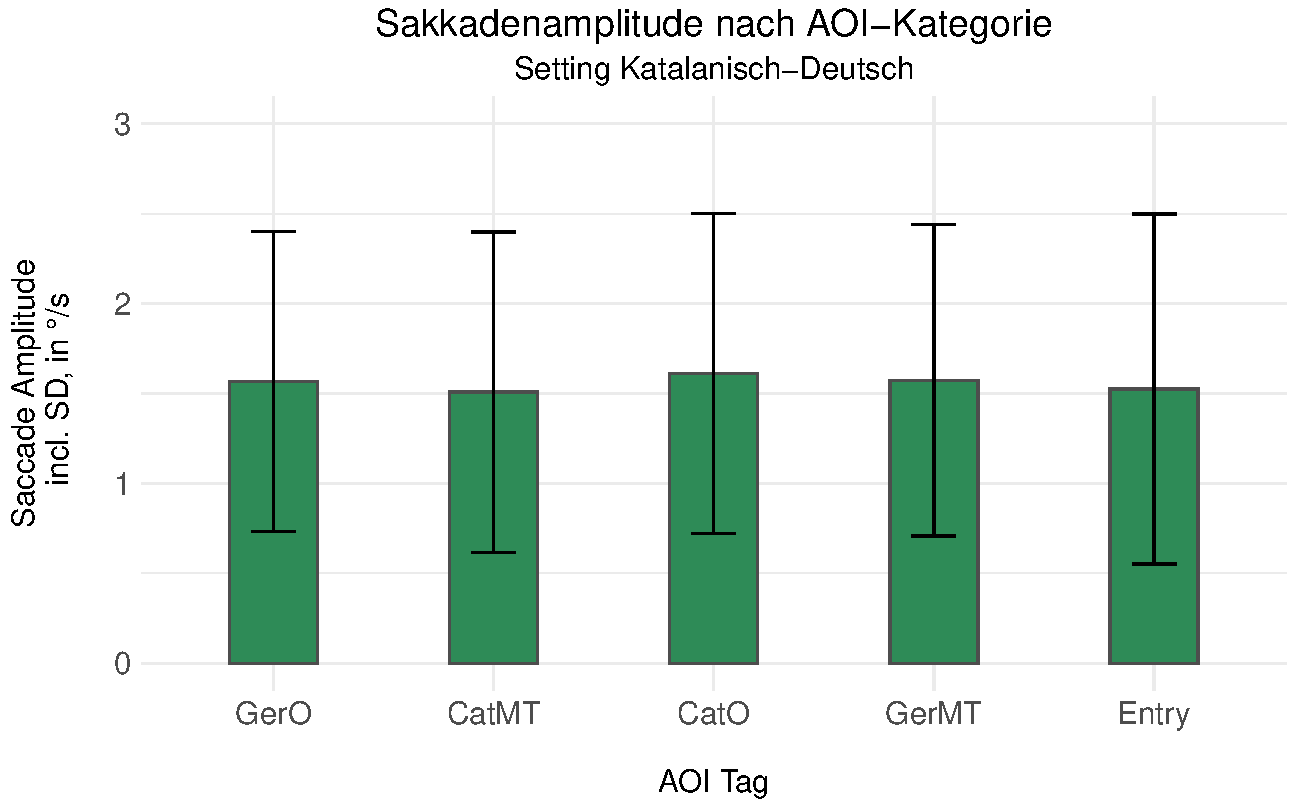
\includegraphics[width=.85\textwidth]{Figures/EyeTracking/CatDe/ggplot_boxplot_sacamp_AOI_de}
	\caption{Sakkadenamplitude pro AOI}
	\label{K6:fig:CatDe:sacamp-box}
\end{figure}

%------------------------------------------------------------------------
\is{Sakkade!-namplitude|)}

%------------------------------------------------------------------------

\subsubsection{Sakkadendauer}
\label{K6:subsubsec:sacdur:CatDe}

%------------------------------------------------------------------------

\is{Sakkade!-ndauer|(}
Der Anderson-Darling-Test\is{Anderson-Darling-Test}\is{Statistik!Testverfahren!Anderson-Darling-Test} zeigt, dass sowohl die Gesamtheit des Datensatzes als auch der Datensatz nach einzelnen AOI-Kategorien in Bezug auf die Sakkadendauer nicht normalverteilt ist. Es ergibt sich für die Gesamtheit ein Verteilungswert im AD-Test von ($A = 3.442,2, p < 0,01$) und für die Kategorien von \emph{GerO}: ($A = 374,99, p < 0,01$), \emph{CatMT}: ($A = 749,75, p < 0,01$), \emph{CatO}: ($A = 510,65,\allowbreak\ p < 0,01$), \emph{GerMT}: ($A = 1.246,5, p < 0,01$) und \emph{Eingabe}: ($A = 537,5, p < 0,01$). Auch eine logarithmische Transformation\is{Statistik!Transformation!logarithmische} änderte die Verteilung nicht wesentlich. Auf die Kategorie \emph{GerO} verfallen in absoluten Zahlen 2.099 Sakkaden, 3.700 auf \emph{CatMT}, 2.491 auf \emph{CatO}, 5.899 auf \emph{GerMT} und 2.883 auf die Eingabemaske. Insgesamt enthält der Datensatz somit 17.072 Sakkaden.


%------------------------------------

\begin{table}
    \begin{tabular}{lccc} 
    \lsptoprule
        {AOI-Kategorie} & {Mittelwert} & {Median} & {SD} \\ 
        \midrule
        GerO   & 31,19 & 21 & 31,64 \\ 
        CatMT   & 34,25 & 20 & 39,59\\ 
        CatO    & 33,44 & 21 & 37,71\\ 
        GerMT  & 30,60 & 20 & 33,97\\ 
        Eingabe  & 38,12 & 22 & 43,76\\ 
        \midrule
        Global  & 33,15 & 21 & 37,41\\ 
        \lspbottomrule
    \end{tabular}
    \caption[Mittelwert, Median und SD der Sakkadendauer]
            {Mittelwert, Median und SD der Sakkadendauer nach AOI-Kategorie\label{K6:tab:CatDe:sacdur}}
\end{table}

%------------------------------------

%------------------------------------------------------------------------

\begin{figure}
    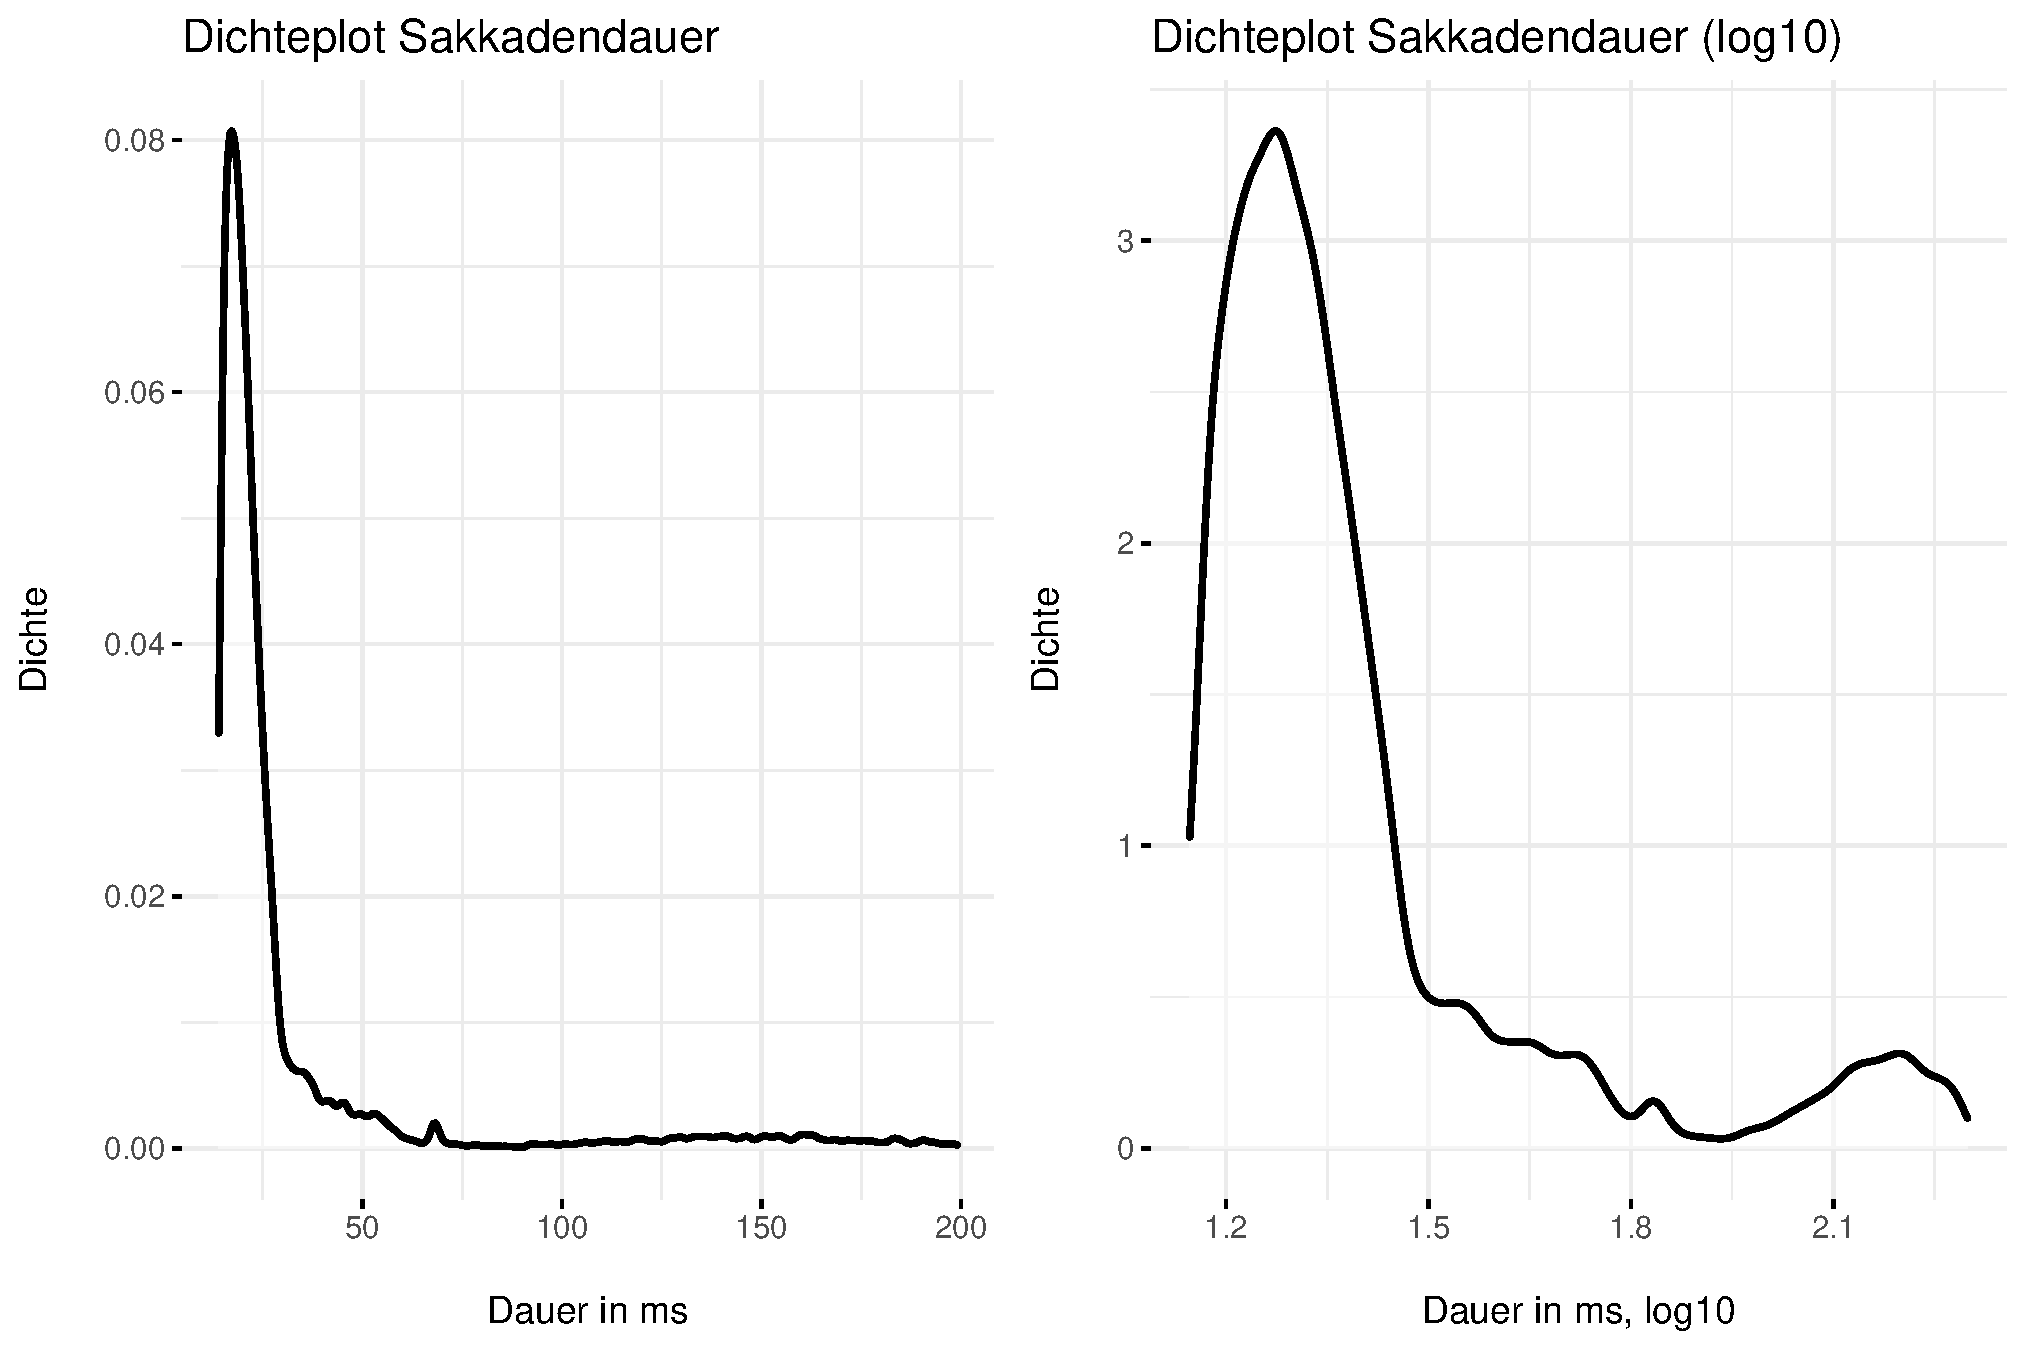
\includegraphics[width=\textwidth]{Figures/EyeTracking/CatDe/ggplot_CatDe-SacDur_density_de}
	\caption{Verteilung der Sakkadendauer: normal (links), logarithmisch transformiert (rechts)}
	\label{K6:fig:CatDe:sacdur-density}
\end{figure}

%------------------------------------------------------------------------

Ein Kruskal-Wallis-Test\is{Kruskal-Wallis-Test}\is{Statistik!Testverfahren!Kruskal-Wallis-Test} belegt, dass Unterschiede bei der Sakkadendauer zwischen den einzelnen Teilnehmer{\textperiodcentered}innen bestehen ($\chi^2(20) = 184,64, p < 0,01$). Anschließend durchgeführte Post-hoc-Tests (Dunn-Benjamini-Hochberg-Tests)\is{Dunn-Benjamini-Hochberg-Test}\is{Statistik!Testverfahren!Dunn-Benjamini-Hochberg-Test} zeigen, dass sich 114 von 210 möglichen Gruppierungen (54,29\,\%) signifikant voneinander unterscheiden, sodass gefolgert werden kann, dass die Sakkadendauer in gewissem Maße von der Individualität der Teilnehmer{\textperiodcentered}innen abhängt.

Ein weiterer Kruskal-Wallis-Test\is{Kruskal-Wallis-Test}\is{Statistik!Testverfahren!Kruskal-Wallis-Test} belegt, dass Unterschiede bei der Sakkadendauer zwischen den einzelnen AOI-Kategorien bestehen ($\chi^2(4) = 49,43,\allowbreak\ p < 0,01$). Anschließend durchgeführte Post-hoc-Tests (Dunn-Benjamini"=Hochberg"=Tests, s. Tab. \ref{tab:CatDe:dunntest-sacdur}, der Asterisk zeigt das Signifikanzlevel an: * $\alpha{} < 0,05$)\is{Dunn-Benjamini-Hochberg-Test}\is{Statistik!Testverfahren!Dunn-Benjamini-Hochberg-Test} zeigen, dass sich 6 von 10 Gruppierungen signifikant voneinander unterscheiden, sodass gefolgert werden kann, dass die Sakkadendauer in gewissem Maße von der AOI-Kategorie abhängt.
Die Effektgröße nach \citet{cohen_power_1992}\is{Cohen!Effektstärke nach}\is{Statistik!Testverfahren!Effektstärke nach Cohen} zeigt dabei keinen Effekt ($r < 0,1$) für alle Gruppierungen.

%------------------------------------

\begin{table}
    \begin{tabular}{lS[table-format=-1.6]S[table-format=1.4]@{ }lc}  
    \lsptoprule
        {AOI-Kategoriepaar} & {$z$} & \multicolumn{2}{c}{$p$ (angepasst)} & {Effekt} \\ 
        \midrule
        CatMT-CatO  & -1,543763 & 0,0767 &  \\   
        CatMT-Eingabe &  -4,700784 &0,0000 & *** & 0,06\\   
        CatO-Eingabe  &  -2,806306 & 0,005 & ** & 0,04 \\   
        CatMT-GerMT & 0,928215 & 0,1963 & \\   
        CatO-GerMT  &  2,489077 & 0,0107 & * & 0,03 \\   
        Eingabe-GerMT &  5,995560 & 0,0000 &*** & 0,06 \\   
        CatMT-GerO  & -3,588229 & 0,0004 & ** & 0,05\\  
        CatO-GerO   & -1,958909 & 0,0358 & \\  
        Eingabe-GerO  & 0,652672 & 0,2570 &  \\  
        GerMT-GerO  & -4,623838 & 0,0000 & *** & 0,05\\
        \lspbottomrule
    \end{tabular}
    \caption{Ergebnisse des Dunn-Tests: Gruppierte Vergleiche der Sakkadendauer nach AOI-Kategorie\label{tab:CatDe:dunntest-sacdur}}
\end{table}

%------------------------------------

Für die Vergleichspaare \emph{CatO-GerO} und \emph{Eingabe-GerO} ergeben sich hingegen keine signifikanten Unterschiede. Der Vergleich der Sakkadendauer ist unauffällig, sodass angenommen werden kann, dass das Erfassen der deutschen Originalbeiträge etwa gleich andauernde Sakkaden hervorruft wie das Betrachten der Eingabemaske oder das Lesen des katalanischen Originals. Auch das Paar \emph{CatMT-CatO} ist unauffällig, sowohl das katalanische Original als auch die MÜ in die Sprache werden also von den Versuchspersonen mit ähnlich langen Sakkaden betrachtet. Die gleiche Feststellung trifft ebenso auf das Paar \emph{CatMT-GerMT} zu.

%------------------------------------------------------------------------

\begin{figure}
    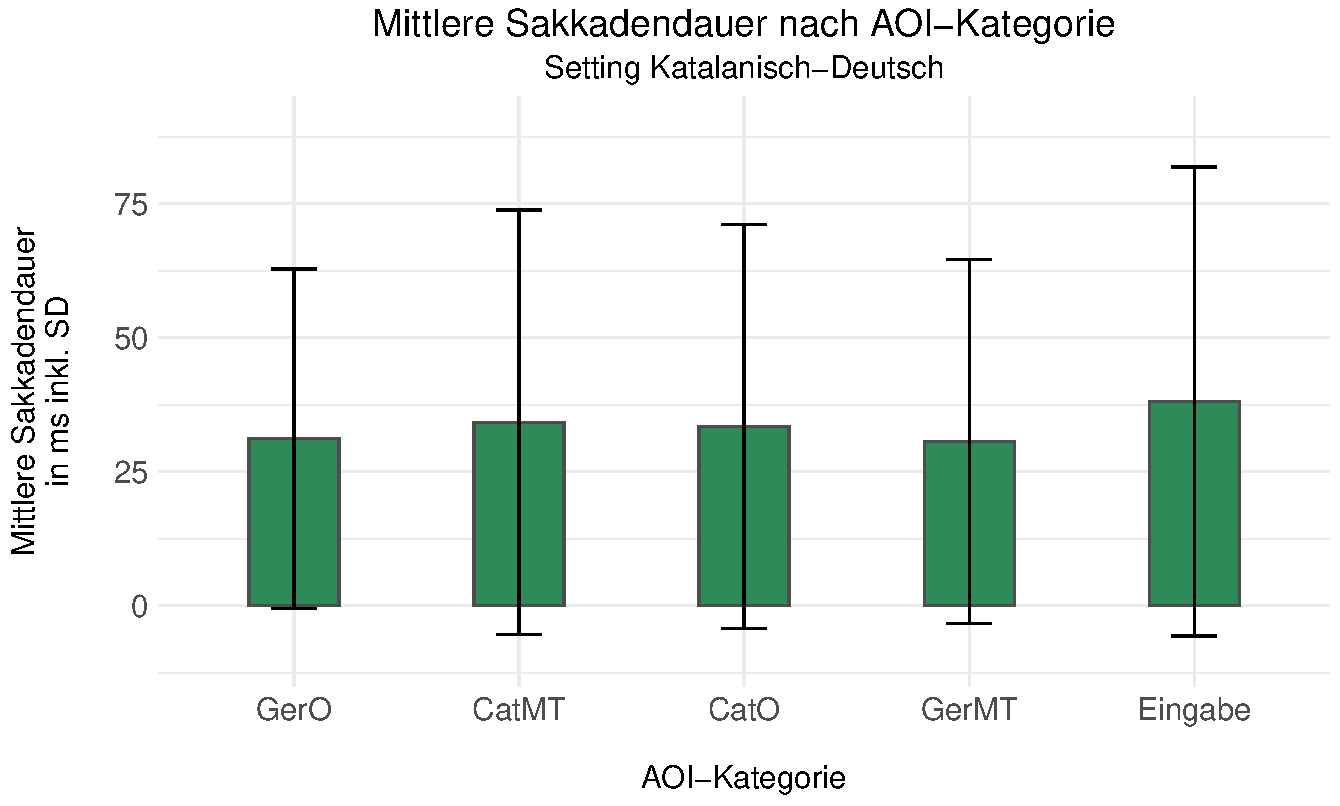
\includegraphics[width=\textwidth]{Figures/EyeTracking/CatDe/ggplot_boxplot_sacdur_AOI_de}
	\caption{Sakkadendauer pro AOI\label{K6:fig:CatDe:sacdur-mean}}
\end{figure}

%------------------------------------------------------------------------
\is{Sakkade!-ndauer|)}

%------------------------------------------------------------------------

\subsection{Zusammenfassung der Ergebnisse im Setting Katalanisch-Deutsch}
\label{K6:subsec:resumee:CatDe}

%------------------------------------------------------------------------

Die Auswertung der beiden Fragebögen jeweils zu Beginn als auch zu Ende der Studie zeugt von einer variabel zusammengesetzten Kohorte. Die teilnehmenden Versuchspersonen sind, mit Ausnahme einer Person, allesamt Studierende der Universität Leipzig. Es handelt sich um junge Menschen Anfang 20, die einerseits mehrere Fremdsprachen sprechen und andererseits auch mehrheitlich bereits Auslandserfahrung aufweisen. Skype\is{Skype}, und noch konkreter: der Skype Translator\is{Skype!Skype Translator}, ist für die Versuchspersonen nicht die präferierte Software für den Kontakt mit Freunden, Familie und anderen Menschen. Zugleich ist der Funktionsumfang von Skype nicht gänzlich unbekannt. Die Auswahl der Versuchsteilnehmer{\textperiodcentered}innen entspricht der von vergleichbaren Studien im Umfeld der Translationsprozessforschung\is{Translationsprozessforschung}. So haben etwa auch \citet{hyona_pupil_1995, beiswenger_eyetracking_2017} auf Studierende zur Durchführung der jeweiligen Studien zurückgegriffen.

Die Rückmeldungen zur Leistung und Qualität\is{Qualität}\is{maschinelle Übersetzung!Qualität der} des Skype Translators\is{Skype!Skype Translator} und der Studiensituation sind schwankend. Einerseits werden mehrere Mängel bei der MÜ-Ausgabe benannt, andererseits geben viele Teilnehmer{\textperiodcentered}innen an, dass der zwischengeschaltete Skype Translator kaum gestört habe bzw. kaum wahrgenommen wurde.

Die Analyse der untersuchten Indikatoren deutet auf Unterschiede bei der Wahrnehmung der einzelnen AOI-Kategorien hin. Sowohl die numerische als auch statistische Untersuchung weist in die Richtung eines Leseverhaltens, das sich wie folgt kennzeichnet: 

Die Erfassung der Ausgabe der maschinellen Übersetzung ins Deutsche ist für die Versuchspersonen kognitiv fordernder als die Betrachtung der eigenen, deutschsprachigen Textnachrichten. Dafür sprechen sowohl numerische Indikatoren wie die Fixations-\is{Fixation!Anzahl der} und Regressionsanzahl\is{Regression!Summe der} oder die Pupillengröße\is{Pupillengröße} als auch temporäre Maße wie die Verweildauer und die Durchlaufdauer\is{Durchlauf!-dauer}. Die Untersuchung der Sakkaden in Form der Amplitude\is{Sakkade!-namplitude} und Dauer\is{Sakkade!-ndauer} ist hingegen -- unter Annahme einer natürlichen Korrelation beider Indikatoren -- zum Teil widersprüchlich und bedarf einer genaueren Betrachtung. Als grundlegende Tendenz kann jedoch auch hier festgestellt werden, dass die Sakkaden sowohl mit Blick auf die Ausrichtung, die Anzahl, die Dauer als auch die Amplitude auf ein unterschiedliches Leseverhalten in Bezug auf die einzelnen AOI-Kategorien deuten.

Die Erkenntnisse, die aus den Daten der Eingabemaske gezogen werden können, sind nur begrenzt interpretierbar. Die Eingabemaske wurde als statisches AOI annotiert, somit sind Indikatoren, die auf ein erstmaliges Ereignis abzielen, auch tatsächlich immer nur als das erstmalige, singuläre Ereignis zu verstehen, selbst wenn die Eingabemaske im weiteren Verlauf der Studie erneut oder insgesamt mehrmals betrachtet wurde. Dazu zählt auch die Pupillengröße, da es mehrere Hinweise darauf gibt, dass die Proband{\textperiodcentered}innen die Eingabemaske nutzen, um ihre Augen ruhen zu lassen. Somit kann es sein, dass die Pupillengröße\is{Pupillengröße}, die auf der Eingabemaske erfasst wird, mehrfach variiert. Die Fixationsanzahl\is{Fixation!Anzahl der} und die Gesamtverweildauer sind hingegen eindeutig messbar und können somit auch ohne Einschränkungen interpretiert werden.


%------------------------------------------------------------------------

\section{Die Proband{\textperiodcentered}innen im Setting Deutsch-Deutsch}
\label{K6:sec:Probandinnen-DeDe}

%------------------------------------------------------------------------

Für die Vergleichsgruppe im Setting Deutsch-Deutsch wurden im Zeitraum zwischen Mai und Dezember 2019 acht regulär eingeschriebene Student{\textperiodcentered}innen an der Universität Leipzig\is{Universität Leipzig} rekrutiert. Auch diese Gruppe erhielt eine Aufwandsentschädigung von jeweils 10 Euro. Die Gesprächspartner{\textperiodcentered}innen waren in diesem Fall Studienfreunde des Verfassers dieser Arbeit. Analog zur Aufgabenstellung im Setting Katalanisch-Deutsch sollten die Proband{\textperiodcentered}innen so tun, als würden sie vom IALT\is{IALT|see{Institu für Angewandte Linguistik und Translatologie}}\is{Institut für Angewandte Linguistik und Translatologie} an den Fachbereich 06 der JGU Mainz\is{Johannes Gutenberg-Universität Mainz}, den FTSK\is{FTSK|see{Fachbereich Sprache, Kultur und Translation}}\is{Fachbereich Sprache, Kultur und Translation} in Germersheim, wechseln. Um Informationen zur Wohnungssuche (und zur Universität usw.) zu erhalten, kontaktierten sie deshalb die jeweilige Person.

\begin{sloppypar}
Wie auch im Setting Katalanisch-Deutsch erhielten die Gesprächspartner{\textperiodcentered}\linebreak[3]innen keinen Fragebogen und wurden ebenfalls nicht okkulometrisch untersucht. Anders als jedoch die Studie im Sprachenpaar Katalanisch-Deutsch erhielten die Proband{\textperiodcentered}innen nur den Eingangs-\is{Fragebogen!Eingangs-}, nicht jedoch den abschließenden Fragebogen\is{Fragebogen!Ausgangs-} (der die Erfahrung mit und Eindrücke vom Skype Translator erhebt). Inklusive Vor- und Nachbereitungszeit sollte die Studiendauer pro Person ca. 35 Minuten betragen, von denen auch hier etwa 15 Minuten auf die Gesprächssituation entfallen sollten.
\end{sloppypar}

Von den eingangs erwähnten acht Proband{\textperiodcentered}innen in diesem Setting musste ein Datensatz ausgeschlossen werden, da dieser durch technische Probleme bei der Aufnahme unbrauchbar geworden war. Die verbleibende Kohorte besteht somit aus sieben Personen: fünf Frauen und zwei Männer im Alter von 19 bis 34 Jahren (\diameter\,23,7 Jahre, Median = 21 Jahre, SD = 4,7). Die Studienfächer der Proband{\textperiodcentered}innen sind in \tabref{K6:tab:TN-Feldstudie-DeDe} aufgeschlüsselt. Im Gegensatz zum anderen Versuchssetting waren in diesem Fall auch Student{\textperiodcentered}innen des IALT zugelassen. Dies ist mit den Erkenntnissen von \citet[]{jakobsen_reading_2017} zu rechtfertigen, die daraufhindeuten, dass das Leseverhalten zum Zwecke des Textverständnisses und beim Übersetzen sich unterscheidet. Da es bei dieser Studie um das reine Textverständnis geht, ist davon auszugehen, dass die Proband{\textperiodcentered}innen mit translatorischem Hintergrund die Ergebnisse nicht verfälschen.


%------------------------------------------------------------------------

\begin{table}
 \begin{tabular}{lccc}
 \lsptoprule
        & {Bachelor} & {Master} & {Staatsexamen}\\ 
        \midrule
  Konferenzdolmetschen & - & 1 & - \\ 
  Übersetzen & 2 & 2 & -\\ 
  Romanische Studien & 2 & 0 & -\\   \midrule
  {gesamt} & 4 & 3 & 0\\  \cmidrule(lr){2-4}
   & \multicolumn{3}{c}{7} \\ 
   \lspbottomrule
 \end{tabular}
 \caption{Studienfächer der Teilnehmer{\textperiodcentered}innen\label{K6:tab:TN-Feldstudie-DeDe}}
\end{table}


%------------------------------------------------------------------------

Alle Studienteilnehmer{\textperiodcentered}innen gaben bei den Fragen nach der Sprache, mit der sie primär aufgewachsen seien sowie der hauptsächlich im Alltag verwendeten Sprache Deutsch an. Eine Person fügte bei zweiter Kategorie noch Englisch und Katalanisch hinzu. Als Sprache im Beruf, ohne dass das Konzept im Fragebogen näher spezifiziert wurde, gaben zwei Personen nur Deutsch, eine Person Deutsch, Katalanisch, Französisch und Englisch und wiederum eine Person Deutsch, Englisch und Spanisch an. Eine weitere gab ausschließlich Englisch an. Die verbleibenden zwei enthielten sich der Antwort.

Die weiteren Fremdsprachen (s.\ \tabref{K6:fig:Fremdspr-Prob-DD} und \tabref{K6:fig:CEFR-Niveau-DD}, S.\,\pageref{K6:fig:CEFR-Niveau-DD}) der Proband{\textperiodcentered}innen fokussieren sich auf den romanischen Sprachraum: Vier Mal wurde Spanisch angegeben, drei Mal jeweils Französisch und Katalanisch, jeweils einmal Latein, Schwedisch, Russisch, Portugiesisch und Russisch. Englisch wurde von vier Personen genannt, wobei eine darüber hinaus keine weiteren Sprachen erwähnte.

Der Eingangsfragebogen ging daraufhin im Weiteren auf die Sprachkompetenz\is{Sprachkompeten} entlang des Europäischen Referenzrahmens für eine Auswahl an romanischen Sprachen (Spanisch, Katalanisch, Galicisch, Italienisch, Französisch und Rumänisch) ein.


%------------------------------------------------------------------------

\begin{figure}
    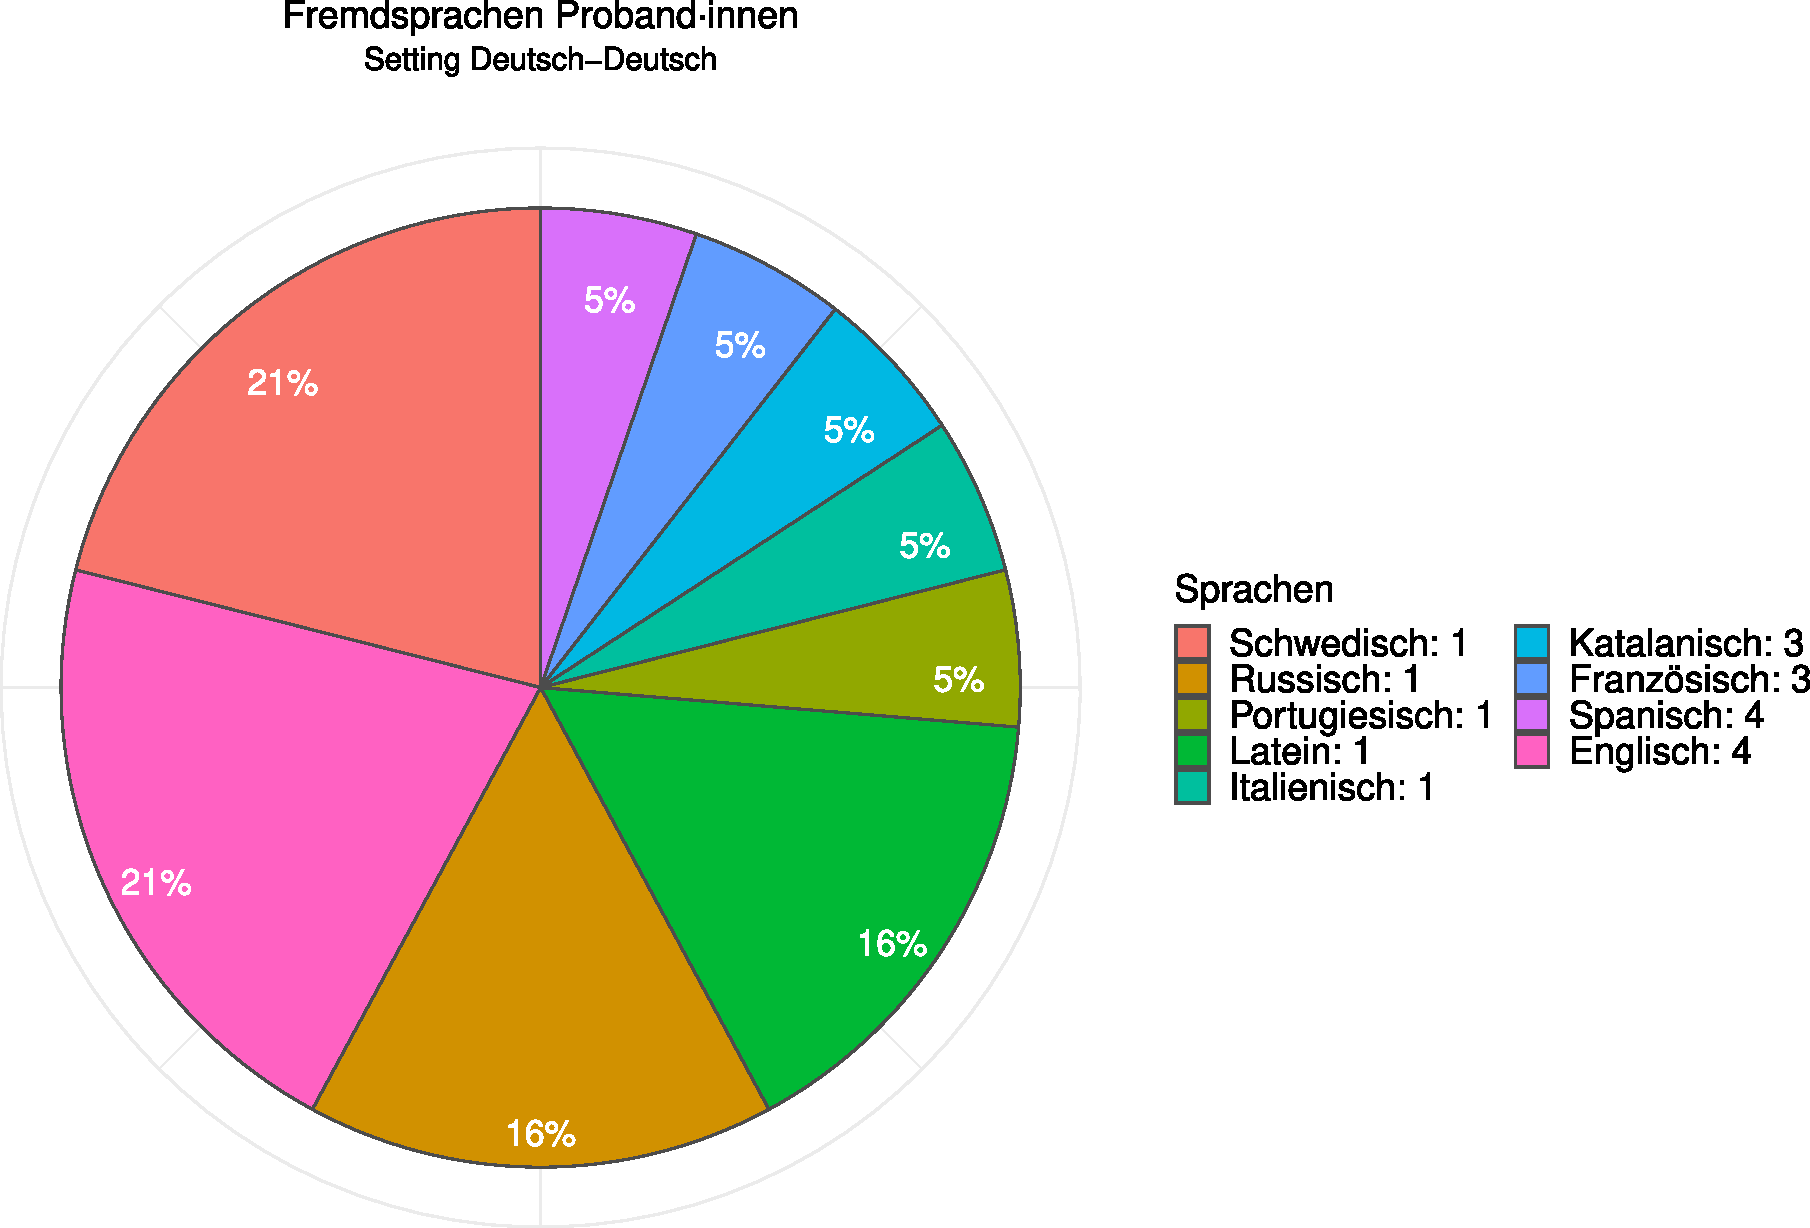
\includegraphics[width=\textwidth]{Figures/EingangsFB/ggplot_sprachen_DeDe_probanden}
	\caption{Fremdsprachen der Proband{\textperiodcentered}innen}
    \label{K6:fig:Fremdspr-Prob-DD}
\end{figure}

%------------------------------------------------------------------------

%------------------------------------------------------------------------

\begin{figure}
    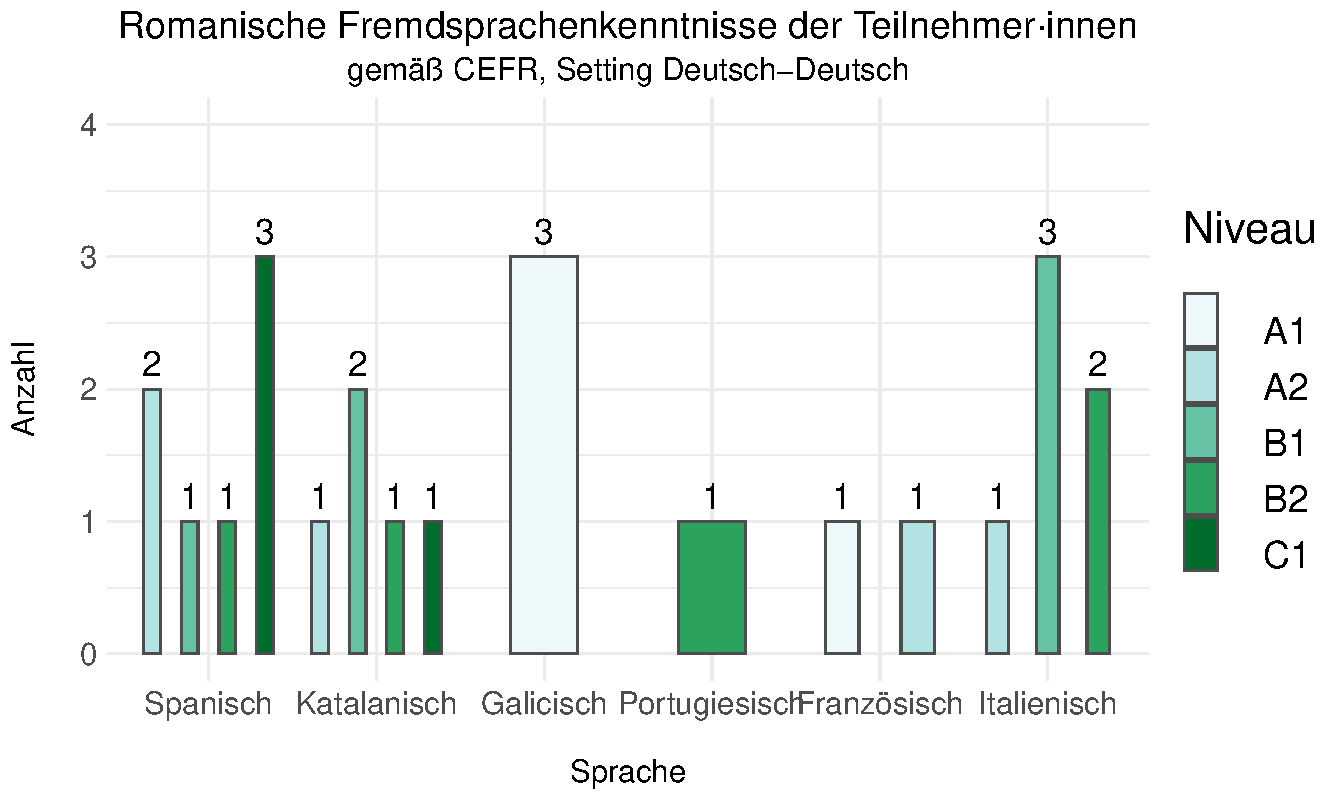
\includegraphics[width=.85\textwidth]{Figures/EingangsFB/ggplot_Fremdsprachen-CEFR-DeDe}
	\caption{Kompetenz in ausgewählten romanischen Sprachen}
    \label{K6:fig:CEFR-Niveau-DD}
\end{figure}

%------------------------------------------------------------------------

Alle Proband{\textperiodcentered}innen gaben weiterhin an, bereits längere Zeit (mehr als vier Wochen Minimum, kein Urlaub) im Ausland verbracht zu haben. Dabei lagen die bereisten Länder der Teilnehmer{\textperiodcentered}innen hauptsächlich in Europa. Mit Brasilien und den Vereinigten Staaten von Amerika gaben lediglich zwei Teilnehmer{\textperiodcentered}innen Ziele außerhalb Europas an. Fünf der sieben Proband{\textperiodcentered}innen haben hingegen bereits längere Zeit in Spanien verbracht. Die in den jeweiligen Ländern verbrachte Dauer reicht von fünf bis 24 Monate (\diameter\,11,1 Monate, Median = 7 Monate, SD = 7,3). Als Gründe wurden Spracherwerb (2/7), Sprachvertiefung (4/7), Kulturkontakt (3/7), ein Pflichtaufenthalt (1/7) sowie die (zeitweise) Verlagerung des Lebensmittelpunktes (1/7) genannt. Dabei lagen die Aufenthalte zwischen drei und 120 Monaten zurück (\diameter\,45,4 Monate, Median = 28 Monate, SD = 44,4).

%------------------------------------------------------------------------

\subsection{Angaben der Proband{\textperiodcentered}innen im Eingangsfragebogen}
\label{K6:subsec:Angaben-Eingang-Probandinnen-DeDe}

%------------------------------------------------------------------------

\is{Fragebogen!Eingangs|(}
\begin{sloppypar}
Von den sieben Proband{\textperiodcentered}innen in der Vergleichsgruppe im Setting Deutsch-Deutsch gaben vier an, Skype\is{Skype} überhaupt zu nutzen. Davon gaben jeweils zwei an, Skype monatlich bzw. seltener als monatlich zu verwenden. Die Nutzungsdauer pro Sitzung belief sich dabei auf entweder bis zu 30 Minuten (2/4), bis zu einer Stunde (1/4) und länger als eine Stunde (1/4). Drei der vier Personen gaben an, Skype für Windows zu verwenden und eine gab an, die Plattform nicht zu kennen.
\end{sloppypar}

In Bezug auf die Nutzung der einzelnen Funktionen gab jeweils eine Person an, den Voice- bzw. den Textchat zu nutzen. Alle vier Teilnehmer{\textperiodcentered}innen nutzten hingegen den Videochat. Aus dem Pool der weiteren Funktionen wurden nur die Bildschirmübertragung und der Konferenzmodus von jeweils einer Person verwendet.

Die Gesprächspartner{\textperiodcentered}innen der Gruppe waren dabei sowohl Mitglieder der Familie im Inland (2/4) als auch im Ausland (2/4). Weiterhin verwendeten drei Teilnehmer{\textperiodcentered}innen den Dienst für die Kommunikation\is{Kommunikation} mit Freunden im Inland und alle vier für den Kontakt mit Freunden im Ausland. Die weiteren Kategorien (berufliche Gesprächspartner{\textperiodcentered}innen und Institutionen jeweils im In- und Ausland) wurden von keiner Person ausgewählt. Die verwendeten Sprachen in diesen Situationen waren dabei Deutsch (4/4) bzw. Katalanisch, Spanisch, Englisch und Portugiesisch mit jeweils einer Angabe.

Wie auch die Proband{\textperiodcentered}innen im Setting Katalanisch-Deutsch gab auch hier keine{\textperiodcentered}r der Versuchsteilnehmer{\textperiodcentered}innen Erfahrungswerte mit dem Skype Translator\is{Skype!Skype Translator} an. Die Erfahrung mit den Funktionen Video-, Voice- und Textchat wurde auf einer Skala von \emph{1\,-\,schlecht} bis \emph{4\,-\,gut} wie folgt bewertet: Zwei Personen haben eher gute Erfahrungen mit dem Textchat gemacht, eine eher schlechte, eine enthielt sich der Antwort. Alle vier Teilnehmer{\textperiodcentered}innen haben eher gute Erfahrungen mit dem Videochat gemacht. Ebenfalls machten zwei eher gute Erfahrungen mit dem Voicechat, die verbleibenden zwei enthielten sich der Antwort.
\is{Fragebogen!Eingangs-|)}

%------------------------------------------------------

\subsection{Nutzung von Alternativen zu Skype}\largerpage
\label{K6:subsubsec:Nutzung-Alternativen-DD}

%------------------------------------------------------------------------

\is{Skype!Alternativen zu}
Die nachfolgenden Angaben beziehen sich nun wieder auf alle sieben Teilnehmer{\textperiodcentered}innen im Setting Deutsch-Deutsch. Mit der Erhebung der verwendeten Alternativen zu Skype begann im Eingangsfragebogen ein neuer Block, zu dem die Teilnehmer{\textperiodcentered}innen direkt weitergeleitet wurden, die die Frage nach der generellen Skype-Nutzung verneint hatten.

Sechs der sieben Proband{\textperiodcentered}innen gaben demnach an, Alternativen zu Skype zu verwenden. Bei der Frage nach der generellen Nutzung (s. \figref{K6:fig:NutzungsVgl-Alternativen-Modus-DD}, linke Abbildung) führt der Dienst WhatsApp als Alternative zu den angebotenen Kommunikationsmodi\is{Kommunikation!-smodus} \emph{Voice}\is{Chat!Voice-}, \emph{Video}\is{Chat!Video-} und \emph{Text}\is{Chat!Text-} mit jeweils fünf, vier und sechs Nennungen. Der am häufigsten genutzte Dienst, aufgeteilt nach Modus, ist bei der Kommunikation über Text und im Voicechat ebenfalls WhatsApp\is{WhatsApp}. Im Modus Videochat nutzten drei der sieben Versuchsteilnehmer{\textperiodcentered}innen Apple Facetime\is{Apple Facetime} (s. \figref{K6:fig:NutzungsVgl-Alternativen-Modus-DD}, rechte Abbildung).

%------------------------------------------------------------------------

\begin{figure}
    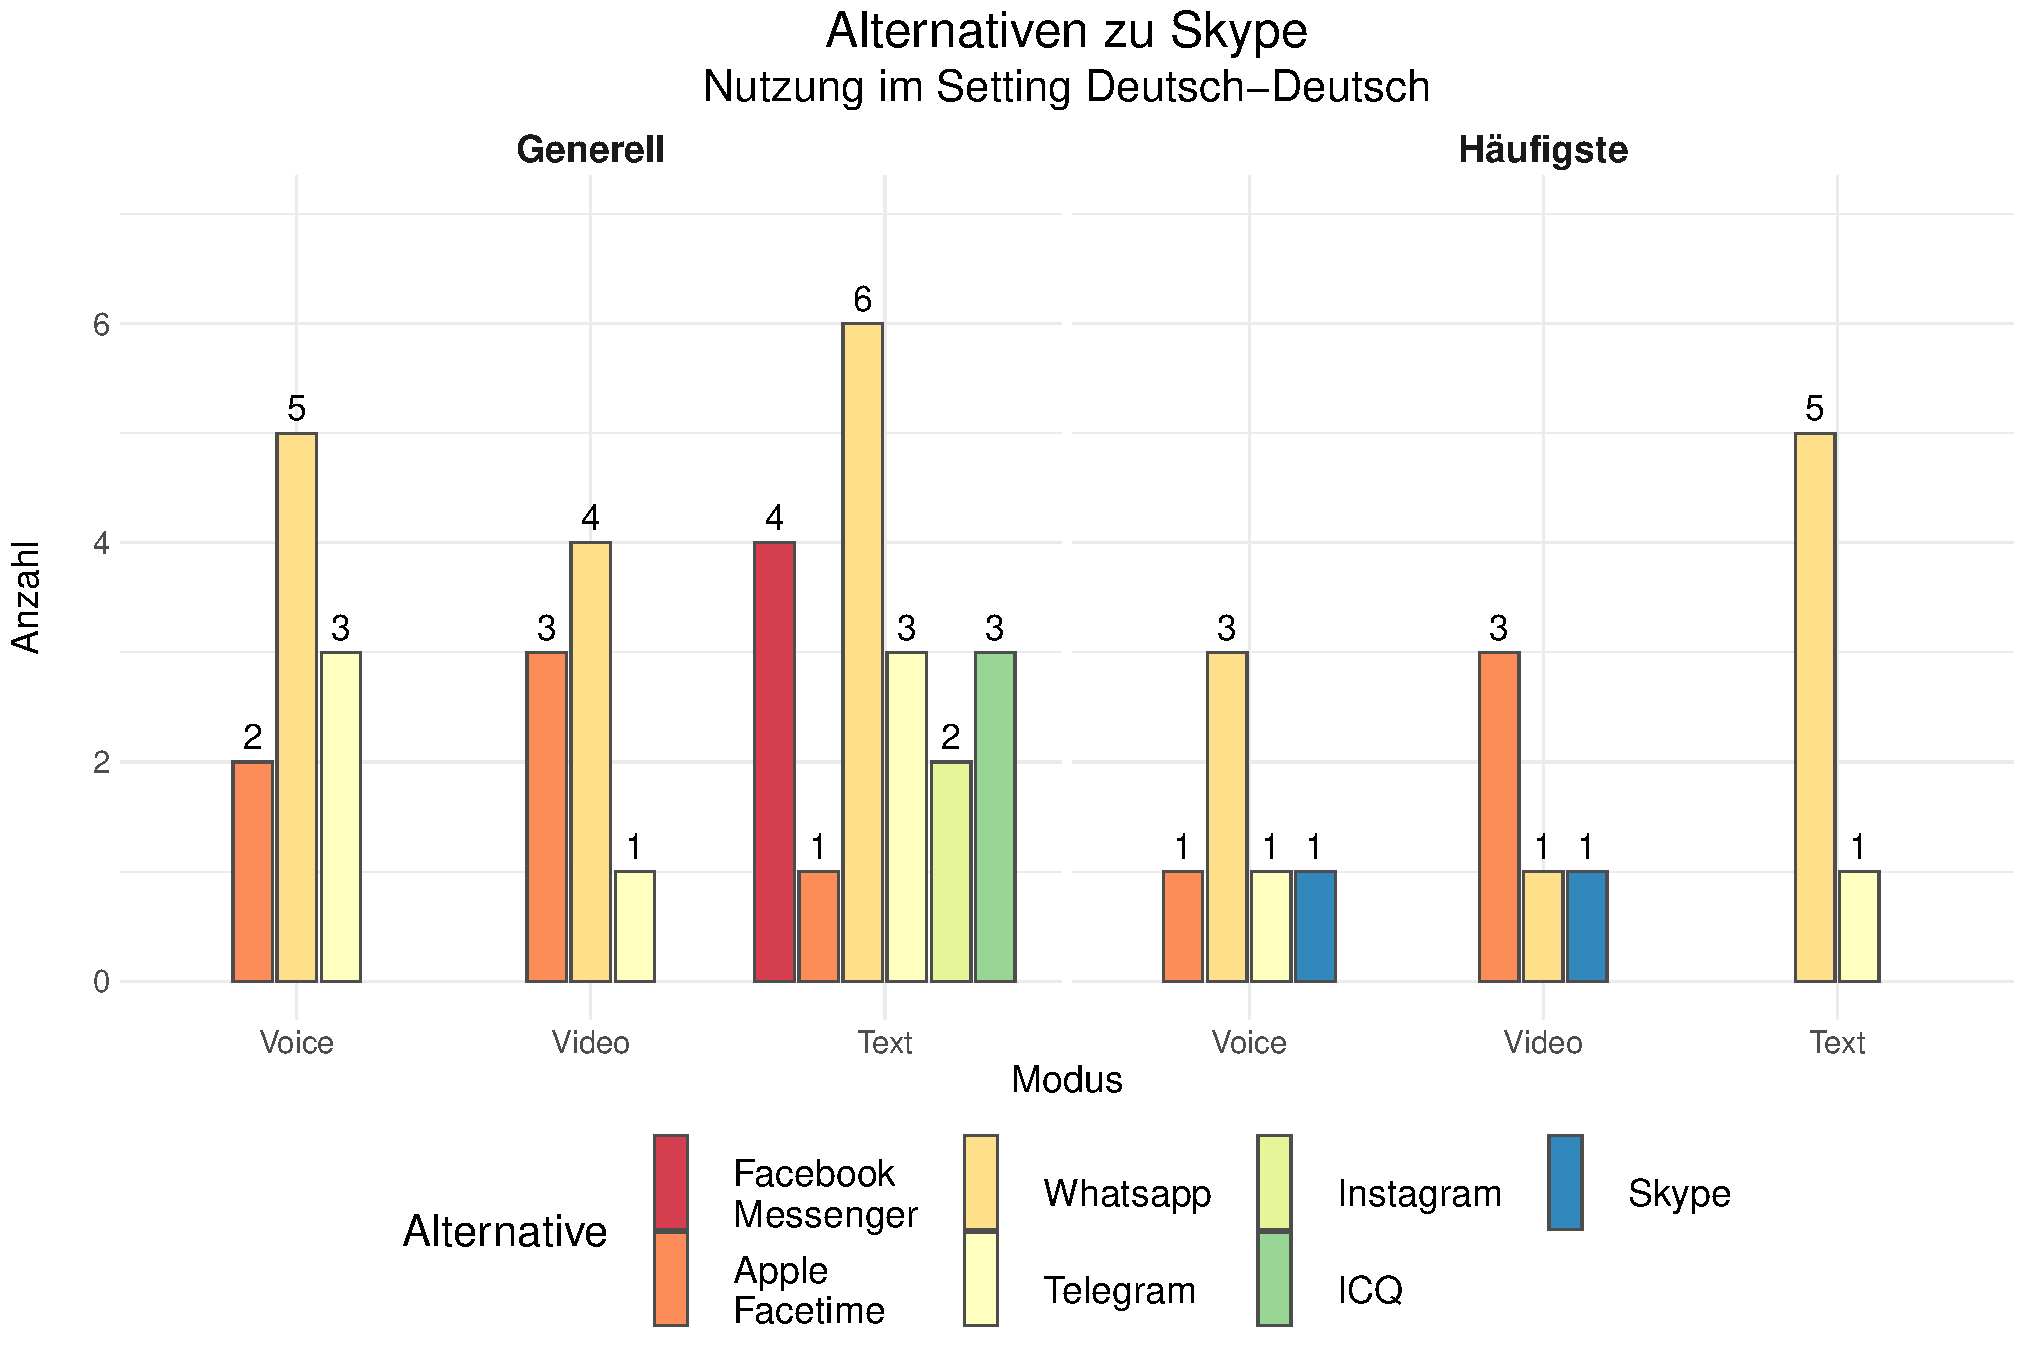
\includegraphics[width=\textwidth]{Figures/EingangsFB/ggplot_skype_Nutzungsvergleich_Alternativen-DeDe}
	\caption{Vergleich: Generelle vs. häufigste Nutzung der Alternativen zu Skype nach Modus}
    \label{K6:fig:NutzungsVgl-Alternativen-Modus-DD}
\end{figure}

%------------------------------------------------------------------------
\is{Skype!Alternativen zu|)}

%------------------------------------------------------------------------

\section{Der Datensatz im Setting Deutsch"=Deutsch}\largerpage[2]

\label{K6:sec:DatenDeDe}

%------------------------------------------------------------------------

%------------------------------------------------------------------------

\subsection{Visuelle Inspektion der Bildschirmmitschnitte}

\label{K6:sub:dede:graph-inspect}

%------------------------------------------------------------------------

Die nachfolgenden Bildschirmfotos (\figref{K6:fig:fixations-DD_TN7}, \ref{K6:fig:sacmove-DD_TN7} und \ref{K6:fig:blinks_DD_TN7}) wurden exemplarisch einer Sitzung im Versuchsaufbau Deutsch-Deutsch entnommen und stellen die Fixationen, Sakkaden und Blinzler während der Kommunikationssituation\is{Kommunikation!-ssituation} dar.

%------------------------------------------------------------------------

\begin{figure}
    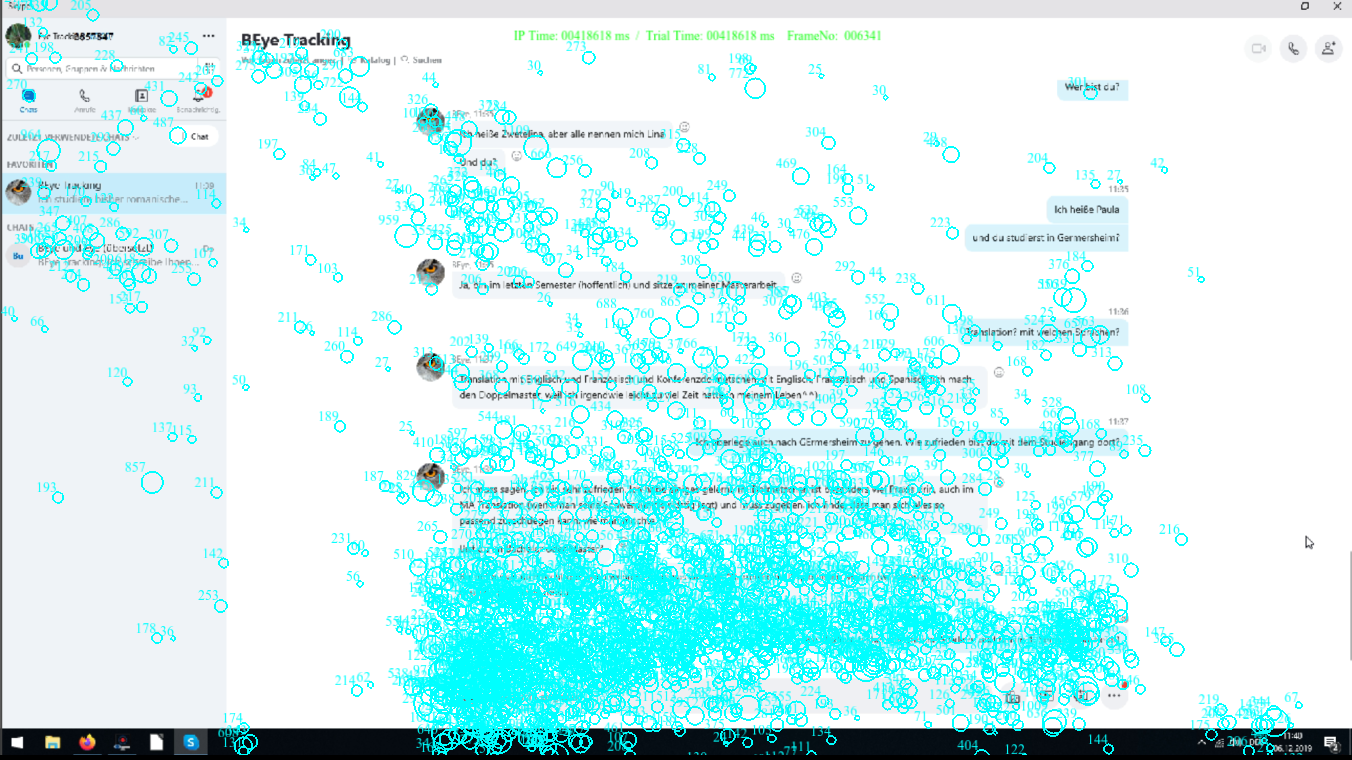
\includegraphics[width=\textwidth]{Figures/Fixmaps/DeDe/Overlay_Image_DD_TN7_Trial_1_Fixations}
	\caption{Fixationen während einer Bildschirmaufnahme}
    \label{K6:fig:fixations-DD_TN7}
\end{figure}


%------------------------------------------------------------------------

Die Fixationen\is{Fixation} sind am unteren Bildschirmrand oberhalb der Eingabemaske besonders dicht verteilt. Sie erstrecken sich über die gesamte Länge des Chat-Bereiches. Mehrere Fixationen sind auch entlang der Kontaktliste und am oberen Bildschirmrand erkennbar, jedoch deutlich weniger häufig und lang als jene im Bereich der eingehenden Nachrichten\is{Nachricht!eingehende}.

%------------------------------------------------------------------------

\begin{figure}
    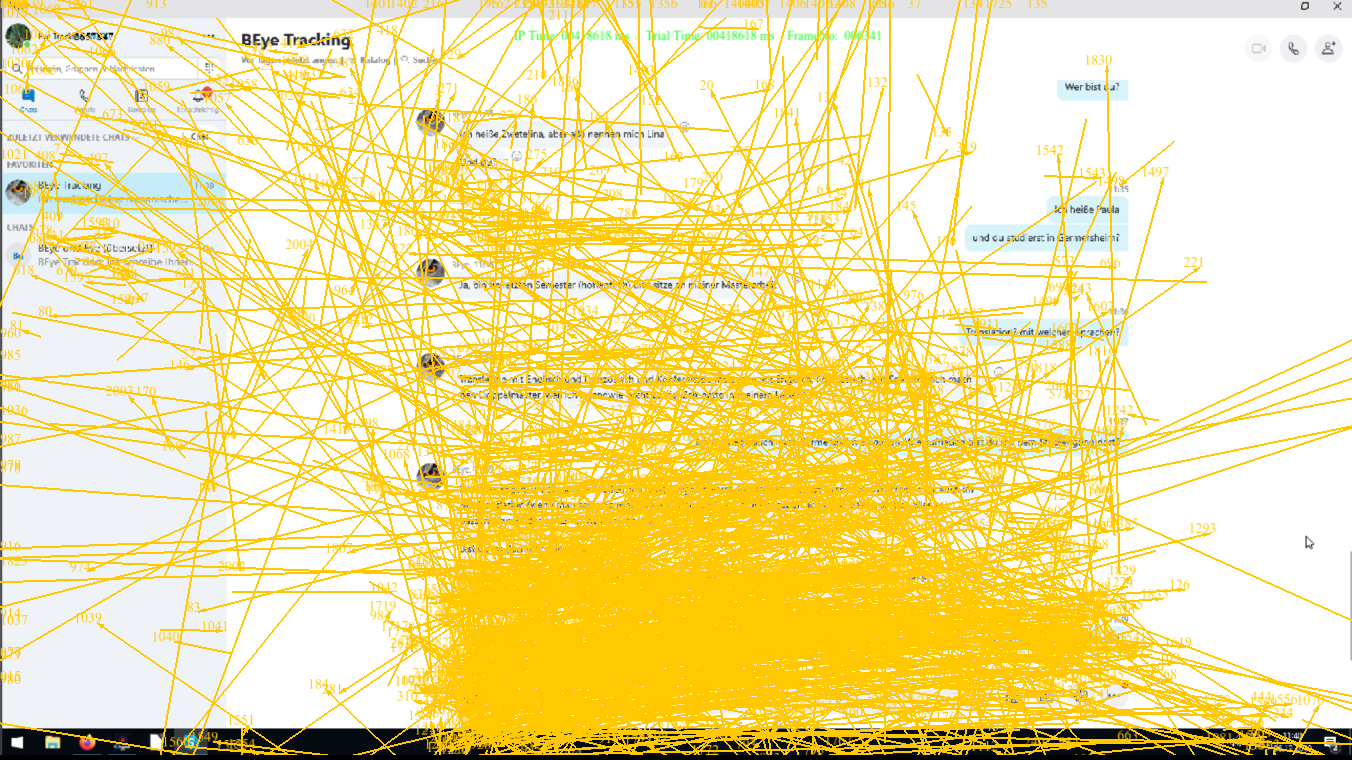
\includegraphics[width=\textwidth]{Figures/Fixmaps/DeDe/Overlay_Image_DD_TN7_Trial_1_Saccades}
	\caption{Sakkaden während einer Bildschirmaufnahme}
    \label{K6:fig:sacmove-DD_TN7}
\end{figure}


%------------------------------------------------------------------------

\begin{sloppypar}
Generell sind über den gesamten Bildschirm, mit Ausnahme der oberen rechten Bildschirmecke, Sakkaden auszumachen. Die Verteilung ist jedoch nicht gleichmäßig, sondern weist eine Konzentration auf: Die visuelle Darstellung der Sakkaden bildet ein sehr dichtes Netz im unteren Bildschirmbereich, oberhalb der Eingabemaske und auf der gesamten Breite des Chatfensters. Die Mehrheit der Sakkaden bleibt in der unteren Bildschirmhälfte. Betrachtet man nur die horizontal ausgerichteten Sakkaden\is{Sakkade!gerichtete}, spricht diese Beobachtung dafür, dass die beteiligten Personen vergleichsweise lange Nachrichten verfasst haben, die jeweils über die Mitte des Chatfensters hinausragen. Die Augenbewegungen im übrigen Bildschirmbereich sind möglicherweise Ausdruck dafür, dass die vielen Sprünge die Wartezeit der Versuchsperson darstellen, während die Person gegenüber eine neue Nachricht verfasst.
\end{sloppypar}

%------------------------------------------------------------------------

\begin{figure}
    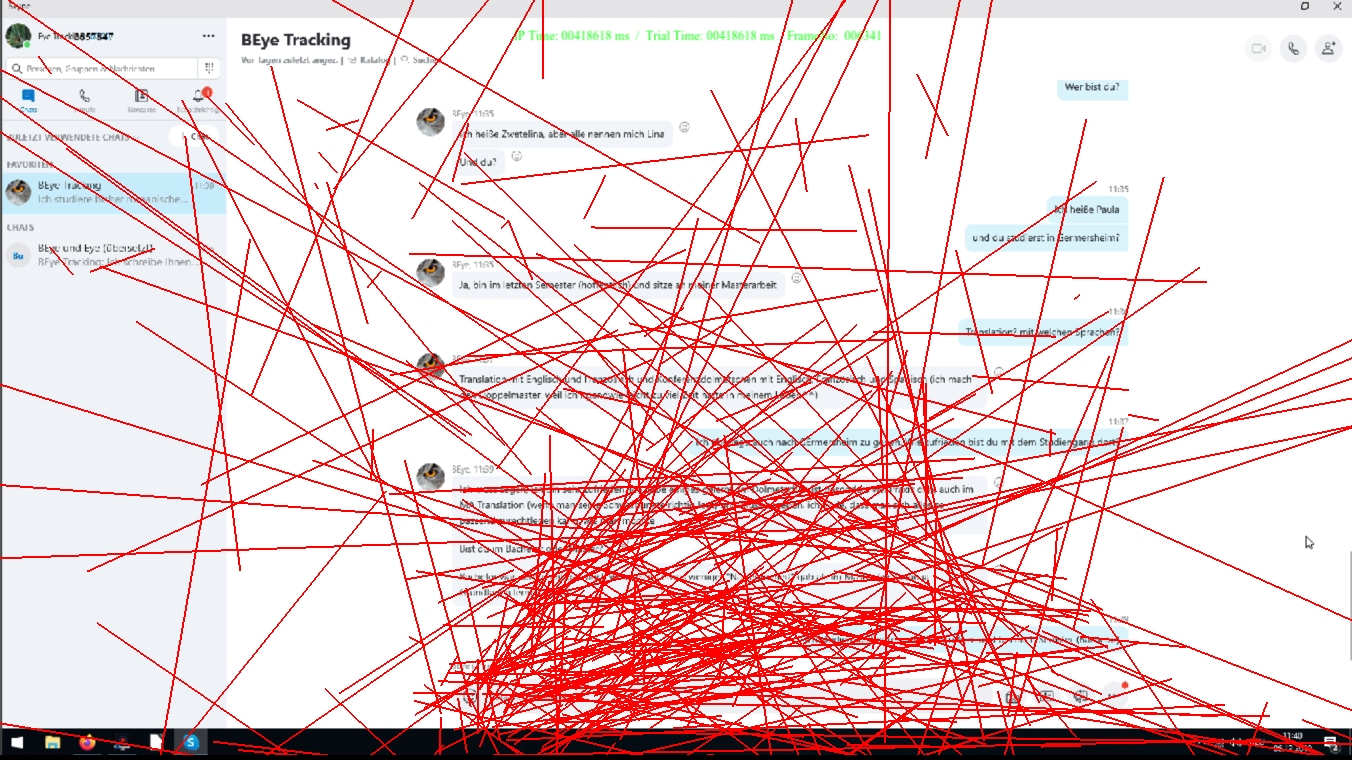
\includegraphics[width=\textwidth]{Figures/Fixmaps/DeDe/Overlay_Image_DD_TN7_Trial_1_Blinks}
	\caption{Blinzler während einer Bildschirmaufnahme}
    \label{K6:fig:blinks_DD_TN7}
\end{figure}


%------------------------------------------------------------------------

Die vom Eye-Tracker erfassten Blinzler\is{Blinzler} konzentrieren sich ebenfalls an der Eingabemaske, dort leicht oberhalb im Bereich mittig links. Wie auch im Falle des anderen Settings können die vermehrt auftretenden Blinzler dafür stehen, dass die Person in diesem Bereich eine stärkere kognitive Auslastung an den Tag gelegt hat. Mehrere Blinzler führen außerdem aus dem erfassbaren Bildschimbereich hinaus. In diesem Fall hat die Versuchsperson möglicherweise auf etwas geachtet, dass sich im Raum, in der die Studie durchgeführt wurde, befand.

%------------------------------------------------------------------------
%%%
%%%
\subsection{Fixationen der Probanden}

\label{K6:sub:FixationenDeDe}
%%%
%%%
%------------------------------------------------------------------------

In \tabref{K6:tab:Werte-ScreenCap-DeDe} sind grundlegende Informationen zu den einzelnen Bildschirmmitschnitten im Setting Deutsch-Deutsch aufgeführt. Wie auch im Setting Ka\-ta\-la\-nisch-Deutsch hat die Mehrheit der Proband{\textperiodcentered}innen länger als die ursprünglich veranschlagten 15 Minuten mit der Textchat-{K}ommunikation\is{Kommunikation!Chat-}\is{Chat!-kommunikation} verbracht. Die Person mit dem Pseudonym DD\_TN1 hat das Gespräch sogar erst nach etwas mehr als 26 Minuten beendet. Jeder einzelne Chatbeitrag\is{Chat!-beitrag} wurde dabei -- wie in Abschnitt~\ref{K5:subsec:Konzept-Feldstudie} (S.\,\pageref{K5:subsec:Konzept-Feldstudie}) dargelegt -- mit einem dynamischen AOI\is{Area of Interest!dynamisches} versehen und entsprechend mit einem Label versehen. Generell schwankt die Anzahl an Beiträgen auf Seiten der Proband{\textperiodcentered}innen zwischen 12 und 23 (\diameter\,18, Median = 19, SD = 3,84) und auf Seiten der Gesprächspartner{\textperiodcentered}innen zwischen 13 und 36 (\diameter\,20, Median = 18, SD = 7,19). Die starken Unterschiede und die hohe Standardabweichung zeugen von einer unterschiedlichen Produktivität und Aktivität während der Kommunikationssitutation\is{Kommunikation!-ssituation}.

% %------------------------------------------------------------------------

% \begin{table}[htbp]
% \centering
% \caption{Durchschnittswerte und Standardabweichung der abhängigen Variablen}
% \label{K6:tab:DD:mean-sd-variables}
%  \begin{tabular}{cccccccc}\hline  
%        \textbf{Variable} & \multicolumn{3}{c}{\textbf{Durchschnitt}} & & \multicolumn{3}{c}{\textbf{Standardabweichung}} \\ \hline
%        & \textbf{A} & \textbf{B} & \textbf{Eingabe} & & \textbf{A} & \textbf{B} & \textbf{Eingabe} 
%        \specialrule{.1em}{.05em}{.05em}
%   IAFFD & 273.56 & 302.22 & 237.29 & & 157.66 & 149.20 & 62.25 \\ \hline 
%   IAFRD & 595.42 & 981.42 & 383.29 & & 661.81 & 953.57 & 250.56 \\ \hline
%   Dwell & 3069.32 & 8081.55 & 45365.00 & & 4908.75 & 8896.20 & 61334.44 \\ \hline
%   IARegPD & 11067.07 & 8282.80 & 2709.50 & & 16635.21 & 10272.36 & 2594.58 \\ \hline
%   IARegInC & 0.76 & 1.67 & 19.43 & & 1.34 & 2.05 & 16.47 \\ \hline
%   IARegOutC & 0.75 & 0.89 & 7.29 & & 1.18 & 1.35 & 19.28 \\ \hline
%  \end{tabular}
% \end{table}

% %------------------------------------------------------------------------

Wie auch im Falle der \emph{fixation heatmaps}\is{Heatmap} im katalanisch-deutschen Versuchsaufbau schauen die Proband{\textperiodcentered}innen überwiegend in das untere linke Drittel des Chatfensters, knapp oberhalb der Eingabemaske. Auch in diesem Setting liegt der Fokus auf der Eingabemaske und dem unmittelbar darüber liegenden Bereich. Anders als die Darstellungen der katalanisch-deutschen Teilnehmer{\textperiodcentered}innen sind die Fokuspunkte hier jedoch raumgreifender und unförmiger.

%------------------------------------------------------------------------


\begin{table}
\begin{tabular}{lcccc}
\lsptoprule
    \multicolumn{3}{c}{} & \multicolumn{2}{c}{{Anzahl Chatbeiträge}} \\ 
    \cmidrule(lr){4-5}
     {Pseudonym} & {Dauer in min} & {Anzahl AOI} & {Eigen} & {Fremd} \\ 
     \midrule
     DD\_TN1 & 26,46 & 27 & 14 & 13 \\ 
     DD\_TN2 & 20,92 & 59 & 23 & 36 \\ 
     DD\_TN4 & 20,27 & 35 & 19 & 16 \\ 
     DD\_TN5 & 17,43 & 30 & 15 & 15 \\ 
     DD\_TN6 & 16,19 & 44 & 22 & 22 \\ 
     DD\_TN7 & 18,93 & 42 & 19 & 23 \\ 
     DD\_TN8 & 16,98 & 30 & 12 & 18 \\ 
     \midrule 
     {Gesamt} & 137,18 & 267 & 124 & 143 \\\cmidrule(lr){4-5}
     \multicolumn{3}{c}{} & \multicolumn{2}{c}{{\diameter\ Anzahl Beiträge (gerundet)}} \\ 
     \multicolumn{3}{c}{} & 18 & 20 \\\cmidrule(lr){4-5}
           \multicolumn{3}{c}{} & \multicolumn{2}{c}{{Median Anzahl Beiträge}} \\
          \multicolumn{3}{c}{} & 19 & 18 \\\cmidrule(lr){4-5}
          \multicolumn{3}{c}{} & \multicolumn{2}{c}{{Standardabweichung (SD)}} \\ 
          \multicolumn{3}{c}{} & 3,84 & 7,19 \\ 
          \lspbottomrule
     \end{tabular}
     \caption{Übersicht Bildschirmaufzeichnungen im Setting De-De}
\label{K6:tab:Werte-ScreenCap-DeDe}
\end{table}



%------------------------------------------------------------------------

\subsubsection{Fixationsanzahl}

\label{K6:subsubsec:fixcount:DD}

%------------------------------------------------------------------------

\is{Fixation!-sanzahl|(}
\tabref{K6:tab:DeDe:mean-sd-fixc} zeigt die aufsummierte Anzahl an Fixationen pro AOI-Ka\-te\-go\-rie. Insgesamt wurden 7.587 Fixationen in den mit AOI versehenen Bereichen erfasst. Der Gesamtschnitt beträgt 30,97 Fixationen pro AOI. Die Beiträge des Gegenübers (\emph{B}) erhielten mit 4.329 Fixationen etwa drei Mal so viele wie die eigenen Nachrichten (1.481). Das Eingabefeld wurde 1.777 Mal fixiert. Der Durchschnittswert für die eigenen Beiträge ist mit 13,97 am kleinsten. Die durchschnittliche Fixationsanzahl auf die Nachrichten des Gegenübers liegt mit 31,8 über dem Gesamtschnitt. Auch die mittlere Anzahl an Fixationen, die auf die Eingabemaske verfallen, liegt über dem Schnitt (253,86).


%------------------------------------


\begin{table}
    \begin{tabular}{l rrrr}  
    \lsptoprule
        AOI-Kategorie & \multicolumn{1}{c}{Summe} & \multicolumn{1}{c}{Mittelwert} & \multicolumn{1}{c}{Median} & \multicolumn{1}{c}{SD} \\\midrule
        A   & 1.481 & 13,97 & 7,5 & 19,50 \\ 
        B   & 4.329 & 31,8 & 19,5 &  42,95\\ 
        Eingabe   & 1.777 & 253,86 & 249,0 & 124,29 \\ 
        \midrule
        Global  & 7.587 & 30,97 & 12,0 & 55,55\\ 
        \lspbottomrule
    \end{tabular}
            \caption[Summe, Mittelwert, Median und SD der Fixationsanzahl]{Summe, Mittelwert, Median und SD der Fixationsanzahl pro AOI-Kategorie\label{K6:tab:DeDe:mean-sd-fixc}}
\end{table}

%------------------------------------

Sowohl die visuelle Inspektion als auch die statistische Untersuchung deuten darauf hin, dass die Fixationsanzahl nicht normalverteilt ist. Ein Shapiro-Wilk-Test ergibt für den gesamten Datensatz ($W = 0,51, p < 0,001$). Eine logarithmische Transformation ändert an dieser Beobachtung nichts (Shapiro-Wilk Test, log10: $W = 0,97, p < 0,001$). Deshalb wird die Fixationsanzahl mit nicht-parametrischen Tests analysiert.

Ein durchgeführter Kruskal-Wallis-Test\is{Kruskal-Wallis-Test}\is{Statistik!Testverfahren!Kruskal-Wallis-Test} deutet auf keine signifikanten Unterschiede bei der Fixationsanzahl nach Teilnehmer{\textperiodcentered}in hin ($\chi^2(6) = 6,88, p = 0,33$). Ein weiterer Kruskal-Wallis-Test\is{Kruskal-Wallis-Test}\is{Statistik!Testverfahren!Kruskal-Wallis-Test} zeigt, dass Unterschiede bei der Fixationsanzahl zwischen den einzelnen AOI-Kategorien bestehen ($\chi^2(2) = 41,32, p < 0,01$). Anschließend durchgeführte Post-hoc-Tests (Dunn-Benjamini-Hochberg-Tests, s. \tabref{K6:tab:DeDe:dunntest-fixcount})\is{Dunn-Benjamini-Hochberg-Test}\is{Statistik!Testverfahren!Dunn-Benjamini-Hochberg-Test} zeigen, dass sich alle Gruppierungen unterscheiden, sodass gefolgert werden kann, dass die Fixationsanzahl von der AOI-Kategorie abhängt. Dabei handelt es sich gemäß der Effektstärke nach \citet{cohen_power_1992}\is{Cohen!Effektstärke nach}\is{Statistik!Testverfahren!Effektstärke nach Cohen} um einen schwachen Effekt (\emph{A-Eingabe}: $r = 0,27$) bzw. mittleren Effekt (\emph{A-B}: 0,34, \emph{B-Eingabe}: 0,39).

%------------------------------------ 



\begin{table}
    \begin{tabular}{lS[table-format=-1.6]S[table-format=1.4]@{ }lS[table-format=1.2]}  
    \lsptoprule
        {AOI-Kategoriepaar} & {$z$} & \multicolumn{2}{c}{$p$ (angepasst)} & {Effekt}\\ 
        \midrule
        A-B       & -5,235690 & 0,0000 & *** & 0,34 \\ 
        A-Eingabe & -4,634883 & 0,0000 & *** & 0,39 \\ 
        B-Eingabe & -2,902860 & 0,0018 & ** & 0,27 \\ 
        \lspbottomrule
    \end{tabular}
    \caption{Ergebnisse des Dunn-Tests: Gruppierte Vergleiche der Fixationsanzahl nach AOI-Kategorie
             \label{K6:tab:DeDe:dunntest-fixcount}}
\end{table}


%------------------------------------

Ein exakter Mann-Whitney-U-Test\is{Mann-Whitney-U-Test}\is{Statistik!Testverfahren!Mann-Whitney-U-Test} wurde verwendet, um Unterschiede bei der Fixationsanzahl pro AOI zwischen beiden Arten der progressiven ersten Fixation\is{Fixation!progressive erste} zu untersuchen. Im Falle des gesamten Datensatzes ergibt der Test ein signifikantes Ergebnis ($U = 6.224,00, p < 0,001, r = 0,22$). Dabei handelt es sich gemäß der Effektstärke nach \citet{cohen_power_1992}\is{Cohen!Effektstärke nach}\is{Statistik!Testverfahren!Effektstärke nach Cohen} um einen schwachen Effekt. Der Median der Fixationsanzahl beträgt 16, wenn die AOI in chronologischer Reihenfolge betreten wurden, und 8, wenn zuvor ein AOI mit höherer Ordnungszahl betrachtet wurde.

\begin{sloppypar}
Unterteilt nach AOI-Kategorie ergibt der Mann-Whitney-U-Test\is{Mann-Whitney-U-Test}\is{Statistik!Testverfahren!Mann-Whitney-U-Test} ebenfalls für die eigenen Chatbeiträge ein signifikantes Ergebnis (AOI-Kategorie \emph{A}: $U = 1.365,5,\allowbreak\ p < 0,05, r = 0,2$). Hierbei beträgt der Median der Fixationsanzahl 8, wenn die Reihenfolge eingehalten wurden, und 6, wenn zuvor ein AOI mit höherer Ordnungszahl betreten wurde. Auch die Testergebnisse für die Chatbeiträge des Gegenübers sind signifikant (AOI-Kategorie \emph{B}: $U = 1.774,5, p < 0,05,\allowbreak\ r = 0,19$). Der Median der Fixationsanzahl bei konsekutiver Betrachtung der AOI beträgt 23, bei ungeordneter Betrachtung 12. Die Effekte sind nach \citet{cohen_power_1992}\is{Cohen!Effektstärke nach}\is{Statistik!Testverfahren!Effektstärke nach Cohen} als schwach einzustufen. Für die Eingabemaske konnten keine Werte berechnet werden, da für die Durchführung des Tests zu wenige Datenpunkte vorlagen.
\end{sloppypar}

Weiterhin korreliert die Fixationsanzahl signifikant mit der Größe der AOI ($r_{s} = 0,77, p < 0,01, n = 570.037$)\is{Spearman's Rho}\is{Korrelationstest nach Spearman}\is{Statistik!Testverfahren!Korrelationstest nach Spearman}. Dabei handelt es sich nach \citet{cohen_power_1992}\is{Cohen!Effektstärke nach}\is{Statistik!Testverfahren!Effektstärke nach Cohen} um einen starken Effekt. Das Bestimmtheitsmaß beträgt 58,89\,\%.

Zur besseren Übersicht sind in \tabref{K6:tab:DeDe:mean-sd-iaarea} die aufsummierte Größe in Pixel der AOI nach Kategorien aufgeführt sowie deren Mittelwert und Standardabweichung. Die mittlere Größe der AOI der eigenen Beiträge ist mit etwa 28.000\,px deutlich geringer als die der Fremdbeiträge mit 40.000\,px. Die Eingabemaske wurde statisch annotiert und ist in jedem einzelenen Datensatz etwa gleich groß. Hier gilt, wie weiter oben bereits problematisiert, die technisch bedingte Einschränkung der Aussagekraft der AOI-Größe (s. Abschnitt~\ref{K5:subsubsec:DynAOI}, S.\,\pageref{K5:subsubsec:DynAOI}). 

%------------------------------------


	
\begin{table}
    \begin{tabular}{lrrr}  
    \lsptoprule
        {AOI-Kategorie} & \multicolumn{1}{c}{Summe} & \multicolumn{1}{c}{Mittelwert} & \multicolumn{1}{c}{SD} \\ 
        \midrule
        A & 2.948.789 & 27.818,76 & 19.384.44 \\ 
        B & 5.342.084 & 40.470,33 & 41.788,15 \\ 
        Eingabe & 481.057 & 68.722,43 & 5.073,75 \\ 
        \midrule
        Gesamt & 8.771.930 & 35.803,79 & 34.211,62 \\ 
        \lspbottomrule
    \end{tabular}
            \caption{Summe, Mittelwert und SD der AOI-Größe in px pro AOI-Kategorie\label{K6:tab:DeDe:mean-sd-iaarea}}
\end{table}

%------------------------------------
\is{Fixation!-sanzahl|)}


%------------------------------------------------------------------------

\subsubsection{Dauer der ersten Fixation}
\label{K6:subsubsec:iaffd:DD}

%------------------------------------------------------------------------

\is{Fixation!Dauer der ersten|(}
Wie in \tabref{K6:tab:DeDe:mean-sd-iaffd} ersichtlich wird, liegt die durchschnittliche Dauer der ersten Fixation auf den eingehenden Nachrichten 25\,ms über dem Gesamtschnitt von 287,29\,ms, wohingegen die Fixationsdauer auf den eigenen Nachrichten 14\,ms unterhalb des Schnittes liegt. Der Wert bei Betrachtung der Eingabemaske liegt 50\,ms unter dem globalen Durchschnitt.

\figref{K6:fig:DD:FFDur-AOI-boxplot} (S.\,\pageref{K6:fig:DD:FFDur-AOI-boxplot}) stellt die Dauer der ersten Fixation pro AOI noch einmal als Boxplot dar. Der Mittelwert pro AOI-Kategorie beträgt für \emph{A}: (\diameter\,273,56 ms, Median: 209\,ms, SD: 157,66), \emph{B}: (\diameter\,302,22\,ms, Median: 274\,ms, SD: 149,20) und \emph{Eingabe}: (\diameter\,237,29\,ms, Median: 249\,ms, SD: 62,25). 

Sowohl die graphische\is{Inspektion!graphische} als auch statistische\is{Inspektion!statistische} Inspektion der Daten belegt, dass keine Normalverteilung vorliegt. Eine logarithmische Transformation\is{Statistik!Transformation!logarithmische} nähert die Verteilung zwar der Gausschen Glockenkurve an, ist jedoch noch immer leicht verschoben (s. \figref{K6:fig:DD:density-ffdur}). Auch eine Berechnung der Schiefe (normal: 1,67, log-transformiert: 0,46) und der Kurtosis\is{Kurtosis} (normal: 3,30, log-transformiert: -0,25) sowie Shapiro-Wilk-Tests (normal: $W = 0,85, p < 0,001$ und log-transformiert: $W = 0,98, p < 0,01$) deuten darauf hin, dass der Datensatz nicht normalverteilt ist. Deshalb werden für die statistische Analyse dieser Daten nicht"=parametrische Tests\is{Statistik!Testverfahren!nicht-parametrisches} verwendet.

%------------------------------------

\begin{table}
    \begin{tabular}{lrrr}  
    \lsptoprule
        {AOI-Kategorie} & \multicolumn{1}{c}{Mittelwert} & \multicolumn{1}{c}{Median} & \multicolumn{1}{c}{SD} \\ 
        \midrule
        A   & 273,56 & 209 & 157,66 \\ 
        B   & 302,22 & 274 & 149,25\\ 
        Eingabe   & 237,29 & 240 &  62,25 \\ 
        \midrule
        Global  & 287,29 & 245 & 151,49\\ 
        \lspbottomrule
    \end{tabular}
            \caption[Mittelwert, Median und SD der Dauer der ersten Fixation]{Mittelwert, Median und SD der Dauer der ersten Fixation pro AOI-Kategorie}
    \label{K6:tab:DeDe:mean-sd-iaffd}
\end{table}

%------------------------------------



%------------------------------------------------------------------------

\begin{figure}
    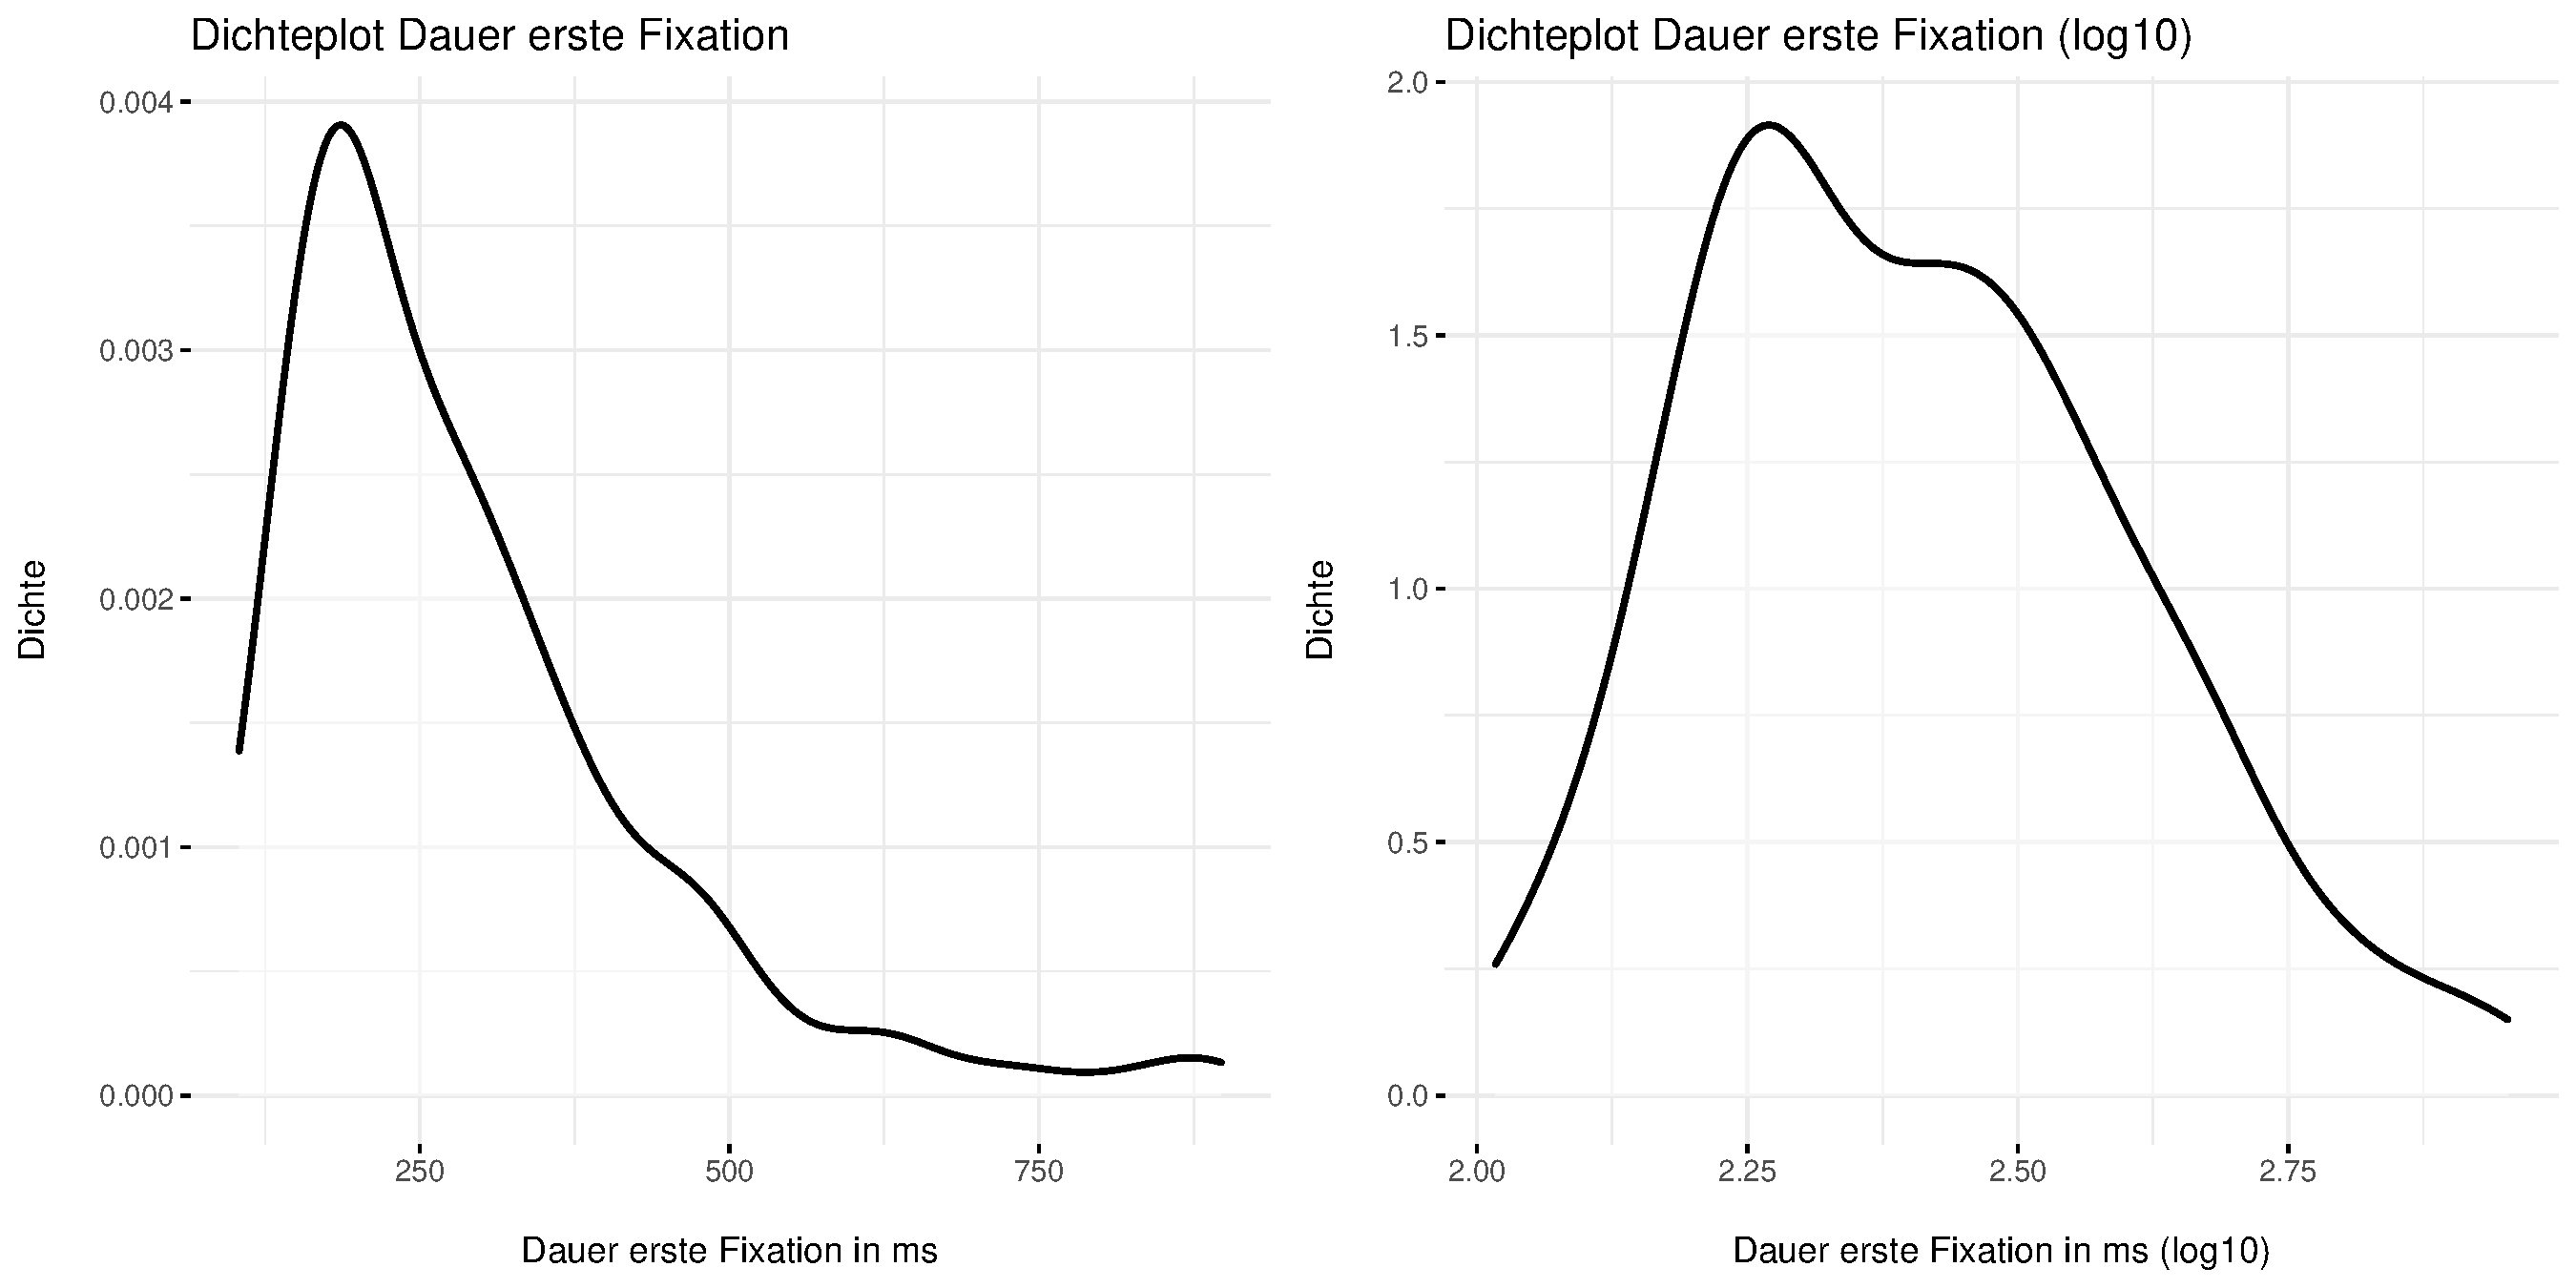
\includegraphics[width=\textwidth]{Figures/EyeTracking/DD/ggplot_DD-FFDur_density_de}
	\caption{Verteilung der Dauer der ersten Fixation: normal (links), 
             logarithmisch transformiert (rechts)\label{K6:fig:DD:density-ffdur}}
\end{figure}

%------------------------------------------------------------------------

\begin{sloppypar}
Ein Kruskal-Wallis-Test\is{Kruskal-Wallis-Test}\is{Statistik!Testverfahren!Kruskal-Wallis-Test} deutet darauf hin, dass Unterschiede in der zentralen Tendenz der Dauer der ersten Fixation zwischen den einzelnen Teilnehmer{\textperiodcentered}innen im Setting Deutsch-Deutsch bestehen ($\chi^2(6) = 17,28, p < 0,01$). Anschließend durchgeführte Post-hoc"=Tests (Dunn-Benjamini"=Hochberg"=Tests)\is{Dunn-Benjamini-Hochberg-Test}\is{Statistik!Testverfahren!Dunn-Benjamini-Hochberg-Test} zeigen, dass sich 7 von 21 möglichen Vergleichspaaren unterscheiden, sodass gefolgert werden kann, dass die Dauer der ersten Fixation teilweise von den Teilnehmer{\textperiodcentered}innen abhängt. Dies ist wenig verwunderlich, bedenkt man, dass die Individualität der Versuchspersonen im Rahmen naturalistisch angelegter Experimente häufig als Zufallseffekte\is{Effekt!Zufalls-} betrachtet werden. Ein zweiter Kruskal-Wallis"=Test\is{Kruskal-Wallis-Test}\is{Statistik!Testverfahren!Kruskal-Wallis-Test} lehnt die Vermutung ab, dass Unterschiede bei der Dauer der ersten Fixation zwischen den einzelnen AOI-Kategorien bestehen ($\chi^2(2) = 4,20, p = 0,12$). Anschließend durchgeführte Post-hoc"=Tests (Dunn-Benjamini"=Hochberg"=Tests, s. \tabref{K6:tab:DeDe:dunntest-ffdur})\is{Dunn-Benjamini-Hochberg-Test}\is{Statistik!Testverfahren!Dunn-Benjamini-Hochberg-Test} belegen ebenfalls, dass keine signifikanten Unterschiede in der Fixationsdauer zwischen den einzelnen AOI bestehen. Allerdings ist der p-Wert in der Gruppe \emph{A-B} niedrig ($z = -1,99, p = 0,07$). Generell kann gefolgert werden, dass die Fixationsdauer nicht von der AOI-Kategorie, also den Chatbeiträgen\is{Chat!-beitrag}, abhängt.\end{sloppypar}

%------------------------------------



\vfill\begin{table}[H]
    \begin{tabular}{lrrr}  
    \lsptoprule
        {AOI-Kategoriepaar} & \multicolumn{1}{c}{$z$} & \multicolumn{1}{c}{$p$ (angepasst)} & \multicolumn{1}{c}{Effekt}\\ 
        \midrule
        A-B       & −1,992319 & 0,07 & - \\ 
        A-Eingabe & 0,080491 & 0,47 & - \\ 
        B-Eingabe & 0,802203 & 0,32 & -\\ 
        \lspbottomrule
        
    \end{tabular}
            \caption{Ergebnisse des Dunn-Tests: Gruppierte Vergleiche der Dauer der ersten Fixation nach AOI-Kategorie}
    \label{K6:tab:DeDe:dunntest-ffdur}
\end{table}


%------------------------------------

%------------------------------------------------------------------------

\begin{figure}[H]
    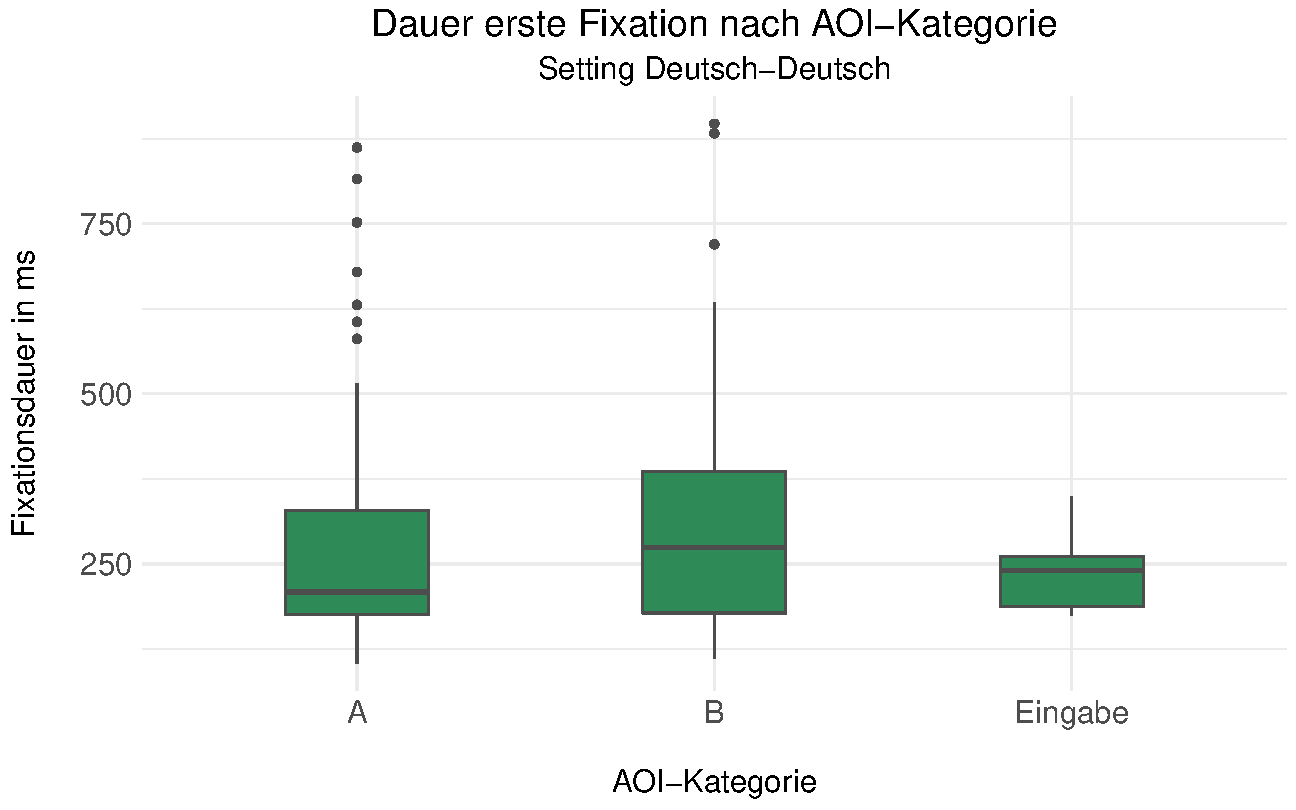
\includegraphics[width=.85\textwidth]{Figures/EyeTracking/DD/ggplot_DD-FFDur_AOI_de}
	\caption{Dauer der ersten Fixation pro AOI-Kategorie
             \label{K6:fig:DD:FFDur-AOI-boxplot}}
\end{figure}\vfill\pagebreak

%------------------------------------------------------------------------

Da die progressive erste Fixation\is{Fixation!progressive erste} nur in zwei Ausprägungen vorliegt (0 und 1), wird nicht der Kruskal-Wallis"=Test, sondern der Mann-Whitney"=U"=Test\is{Mann-Whitney-U-Test}\is{Statistik!Testverfahren!Mann-Whitney-U-Test} verwendet. Es besteht ein signifikanter Unterschied in der zentralen Tendenz der Dauer der erstmaligen Fixation zwischen den AOI, bei denen zuvor ein AOI mit höherer Ordnungszahl betrachtet wurde, und denen, die chronologisch betreten wurden. Die eigenen Chatbeiträge\is{Chat!-beitrag} der Versuchspersonen werden kürzer fixiert, wenn zuvor ein AOI mit höherer Ordnungszahl betrachtet wurde, als wenn es sich um eine tatsächliche chronologische erstmalige Fixation handelt. Ein exakter Mann-Whitney"=U-Test ($U = 1.034,5, p < 0,05, r = 0,24$) in Verbindung mit einer Untersuchung der Effektstärke nach \citet{cohen_power_1992}\is{Cohen!Effektstärke nach}\is{Statistik!Testverfahren!Effektstärke nach Cohen} zeigt dabei allerdings nur einen schwachen Effekt.

%------------------------------------



\begin{table}
    \begin{tabular}{lrS[table-format=1.2{*}]r} 
    \lsptoprule
        {AOI-Kategorie} & \multicolumn{1}{c}{$U$} & \multicolumn{1}{c}{$p$ (angepasst)} & \multicolumn{1}{c}{Effekt} \\ 
        \midrule
        A & 1.034,5 & 0,02{*} & 0,24 \\ 
        B  & 1.689,0 & 0,6 & -\\ 
        Eingabe & n/a & {n/a} & -\\ 
        \midrule
        Global & 5.596,5 & 0,08 & -\\ 
        \lspbottomrule
    \end{tabular}
            \caption[Ergebnisse des Mann-Whitney-U-Tests zur Dauer der ersten Fixation]
                    {Ergebnisse des Mann-Whitney-U-Tests zur Dauer der ersten Fixation nach AOI-Kategorie und progressiver ersten Fixation
                    \label{K6:tab:DeDe:mwutest-ffdur-ffixpro}}
\end{table}


%------------------------------------

Ein Korrelationstest (Spearman’s Rho)\is{Spearman's Rho}\is{Korrelationstest nach Spearman}\is{Statistik!Testverfahren!Korrelationstest nach Spearman} belegt, dass keine signifikanten Zusammenhänge zwischen Dauer der ersten Fixation und der Größe der AOI bestehen ($r_{s} = -0,03, p = 0,68, n = 483.293$).
\is{Fixation!Dauer der ersten|)}

%------------------------------------------------------------------------

\subsubsection{Regressionen}
\label{K6:Subsubsec:regression:dede}

\subsubsubsection{Eingehende Regressionen}
\label{K6:para:DeDe:regin}

%------------------------------------------------------------------------

\is{Regression!eingehende|(}\figref{K6:fig:DeDe:RegIn-AOI-Count} und \tabref{K6:tab:DeDe:mean-sd-regin} zeigen die aufsummierte Anzahl aller Regressionen in ein AOI nach Kategorie sowie deren Mittelwert und Standardabweichung. Die Kategorie \emph{B}, also die Beiträge des Gegenübers, erhielten mit 221 (\diameter\,1,67, SD: 2,05) die meisten Regressionen. In die Kategorien \emph{A} und \emph{Eingabe} fielen jeweils 81 (\diameter\,0,76, SD: 1,35) bzw. 136 (\diameter\,19,43, SD: 16,47) Regressionen. Auffällig sind die Durchschnittswerte, bei denen mindestens eine Regression in die Beiträge des Gegenübers ausgeführt wird und in die Eingabemaske sogar durchschnittlich mehr als 19.


\begin{figure}
    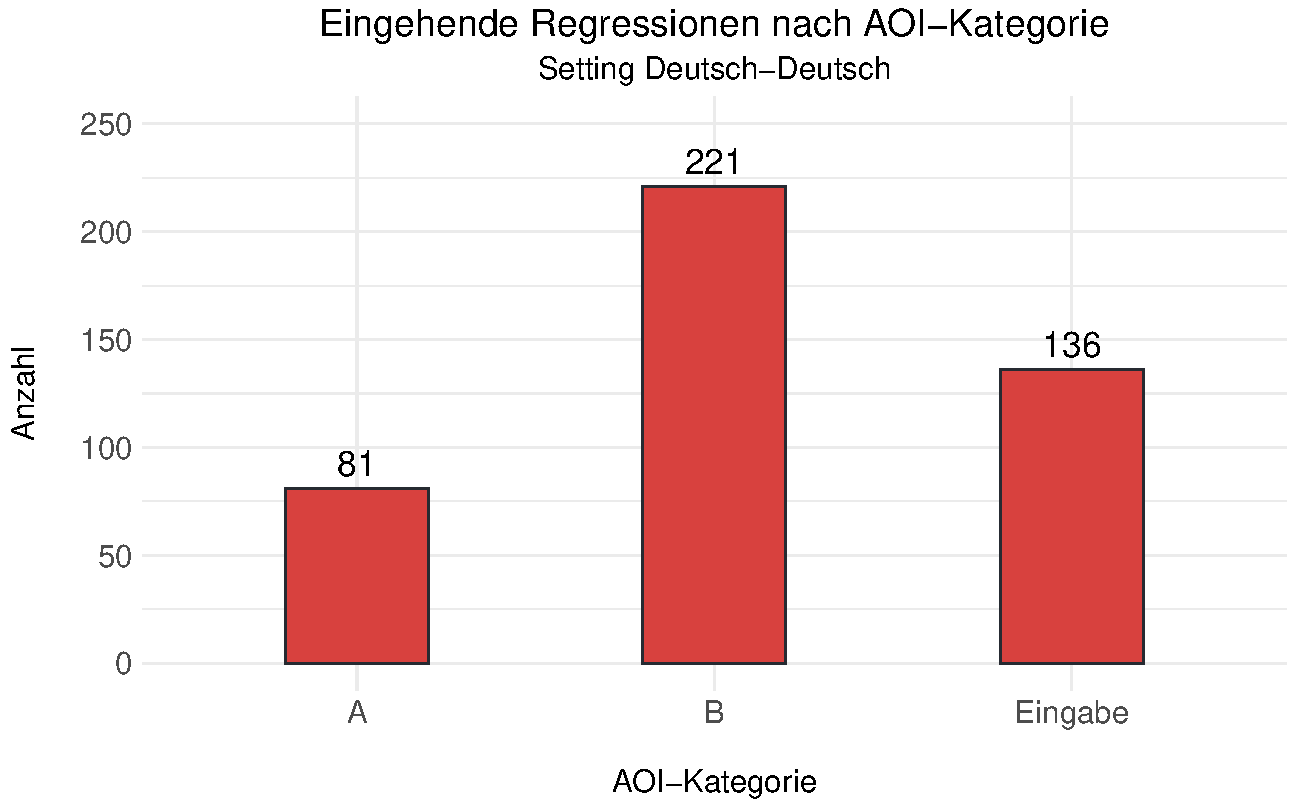
\includegraphics[width=.85\textwidth]{Figures/EyeTracking/DD/ggplot_regression_DD_IN_AOI_de}
	\caption{Anzahl Regressionen in ein AOI\label{K6:fig:DeDe:RegIn-AOI-Count}}
\end{figure}

\begin{table}
    \begin{tabular}{lrrr} 
    \lsptoprule
        {AOI-Kategorie} & \multicolumn{1}{c}{Summe} & \multicolumn{1}{c}{Mittelwert} & \multicolumn{1}{c}{SD} \\
        \midrule
        A  &  81 & 0,76 & 1,35 \\ 
        B &  221 &  1,67 & 2,05 \\ 
        Eingabe  & 136 & 19,43 & 16,47 \\ 
        \midrule
        Global  & 438 & 1,79 & 4,37 \\ 
        \lspbottomrule
    \end{tabular}
    \caption{Summe, Mittelwert und SD der eingehenden Regressionen pro AOI-Kategorie
             \label{K6:tab:DeDe:mean-sd-regin}}
\end{table}

Zur statistischen Untersuchung der Regressionen in ein AOI wurde mit einem binomialen logistischen Regressionsmodell\is{Regressionsmodell!binominales logistisches}\is{Statistik!Testverfahren!Regressionsmodell} mit gemischten Effekten\is{Effekt!gemischter} gearbeitet, das die Teilnehmer{\textperiodcentered}innen (\emph{SessionLabel}) als Zufallseffekte\is{Effekt!Zufalls-} beinhaltete (s. \tabref{K6:tab:DeDe:RegIn-Modell-Stats}). Die Variablen wurden in einer bedingten Vorwärtsauswahl in das Modell integriert. Das simpelste und zugleich genauste Modell erweist sich dabei, ebenso wie einzelne Koeffizienten der integrierten Variablen, als signifikant und liefert bessere Ergebnisse als ein einfaches lineares Regressionsmodell\is{Regressionsmodell!lineares}\is{Statistik!Testverfahren!Regressionsmodell} ($\chi^2(5) = 60,75, p < 0,001$). Zugleich zeigt sich, dass das Modell noch nicht optimal angepasst (C: 0,79, Somers’ D\textsubscript{XY}: 0,58) ist. Während die Kategorien \emph{Intercept} (in diesem Fall \emph{A}) bzw. \emph{Eingabe} keinen Effekt auf die Wahrscheinlichkeit haben, dass eine Regression in ein AOI gemacht wird, steigt die relative Wahrscheinlichkeit bei \emph{B} um 128\,\%. Weiterhin steigt die Wahrscheinlichkeit um 281\,\% mit der Größe der AOI. Hingegen nimmt die relative Wahrscheinlichkeit mit jeder Einheit der \emph{IARegPD} um 35\,\% und mit jeder progressiven ersten Fixation\is{Fixation!progressive erste} um 66\,\% ab.


%------------------------------------

\begin{table}
    \sisetup{table-align-text-after=false}
    \small
    \fittable{\begin{tabular}{lS[table-format=-1.4]S[table-format=1.7]S[table-format=2.2]S[table-format=2.4]S[table-format=-1.3]S[table-format=<1.5{***}]}
    \lsptoprule
         & {Gruppen} & {Varianz} & {SD} & {L.R. X2} & {DF} & {Pr}\\\midrule 
    Zufallseffekt(e) &	{SessionLabel} &	0 &	0 &	60,75 &	1 &	< 0,05{*} \\\midrule
    Fixe Effekt(e) &	{Schätzung} &	{VIF} &	{OR} &	{SE} &	{$z$} & {$\text{Pr}(>z)$}\\\midrule
    (Intercept) &	0,4712 	& &	1,60 &	0,3257 	& 1,447 &	0,14796 \\
    IATagB &	0,8254 &	1,0329236 &	2,28 &	0,2995 &	2,755 &	0,00586{**}\\
    IATagEingabe &	3,1416 &	1,6200961 &	23,14 &	2,7880 &	1,127 &	0,25981\\
    IAFFixPro1 &	-1,0749 &	1,0751683 &	0,34 &	0,3474 &	-3,094 &	0,00197{**} \\
    IARegPD\_z &	-0,4271 &	1,7490922 &	0,65 &	0,2588 &	-1,650 &	0,09896{.} \\
    IA\_AREA\_z &	1,3367 &	1,0849144 &	3,81 &	0,2487 &	5,374 &	< 0,001{***} \\\lspbottomrule
    \end{tabular}}\medskip\\
    \begin{tabular}{lS[table-format=<3.6{***}]}
    \lsptoprule
    {Model statistics} 	&	{Wert} \\\midrule
    {No. Groups} &	7 \\
    {Number of cases in model}	&	245 \\
    {Observed misses} 	& \\	
    {Observed deviance} &	272,6 \\
    {Residual deviance} &	\\
    {R2 (Nagelkerke)} 	&	0,295369 \\
    {R2 (McFadden)} 	&	0,182236 \\
    {R2 (Cox \& Snell)} &	0,219609 \\
    {C} 				&	0,79 \\
    {Somers' D\textsubscript{XY}} &		0,58 \\
    {AIC} 	&	286,6 \\
    {BIC} 	&	311,1 \\
    Prediction accuray & \\	
    Model Likelihood Ratio Test\\
    x2: & 60,75\\
    df:& 5 \\
    $p$ & < 0,001{***} \\
    \lspbottomrule
    \end{tabular}
    \caption[Werte des Regressionsmodells für eingehende Regressionen]
            {Werte des Regressionsmodells für eingehende Regressionen 
             im Setting Deutsch-Deutsch\label{K6:tab:DeDe:RegIn-Modell-Stats}}
\end{table}


%------------------------------------


Wie auch im katalanisch-deutschen Versuchsaufbau wurde zur Überprüfung der Plausibilität\is{Plausibilität} mit nicht-parametrischen Tests\is{Statistik!Testverfahren!nicht-parametrisches} gearbeitet. Bei eingehenden Regressionen im Setting Deutsch-Deutsch deutet ein Chi-Quadrat"=Test\is{Statistik!Testverfahren!Chi-Quadrat-Test} auf ein signifikantes Verhältnis zwischen den jeweiligen AOI-Kategorien und den eingehenden Regressionen hin ($\chi^2(2) = 16,91, p < 0,001$). Weiterhin besteht ein enger Zusammenhang zwischen den eingehenden Regressionen und der progressiven ersten Fixation\is{Fixation!progressive erste} sowohl bei Betrachtung des gesamten Datensatzes ($\chi^2(1) = 6,19, p < 0,05$) als auch der AOI-Kategorie \emph{A} ($\chi^2(1) = 10,84, p < 0,001$)\is{Statistik!Testverfahren!Chi-Quadrat-Test}. Alle weiteren Variablen sind unauffällig.
\is{Regression!eingehende|)}

%------------------------------------------------------------------------

\subsubsubsection{Ausgehende Regressionen}
\label{K6:para:regout:DD}

%------------------------------------------------------------------------

\is{Regression!ausgehende|(}\figref{K6:fig:DeDe:RegOut-AOI-Count} und \tabref{K6:tab:DeDe:mean-sd-regout} zeigen die aufsummierte Anzahl aller Regressionen\is{Regression!Summe der} aus einem AOI sowie deren Mittelwert und Standardabweichung. Aus der Kategorie \emph{B}, also von den Chatbeiträgen\is{Chat!-beitrag} des Gegenübers, wurden mit 118 (\diameter\,0,89, SD: 1,35) die meisten Regressionen getätigt. Aus den Kategorien \emph{A} und \emph{Eingabe} wurden jeweils 79 (\diameter\,0,75, SD: 1,18) bzw. 51 (\diameter\,7,29, SD: 19,28) Regressionen vorgenommen. Aus den beiden Nachrichtenkategorien wird im Schnitt weniger als eine Regression ausgeführt. Anders verhält es sich bei der Eingabemaske, aus der durchschnittlich sieben Regressionen getätigt werden, auch wenn der absolute Wert der niedrigste in diesem Fall ist.

\begin{figure}
    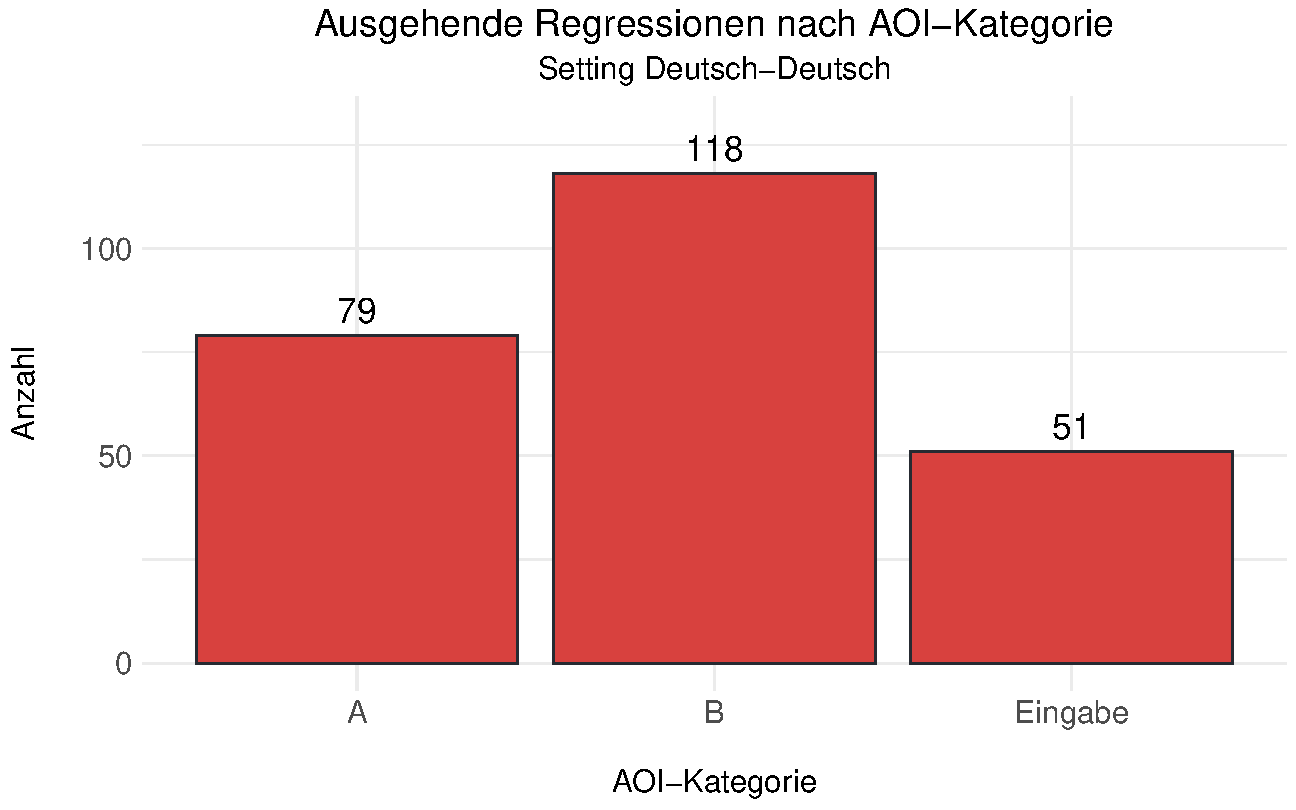
\includegraphics[width=.85\textwidth]{Figures/EyeTracking/DD/ggplot_regression_DD_OUT_AOI_de}
	\caption{Anzahl Regressionen aus einem AOI\label{K6:fig:DeDe:RegOut-AOI-Count}}
\end{figure}

%------------------------------------------------------------------------


%------------------------------------

\begin{table}
    \begin{tabular}{lrrr}
    \lsptoprule
        {AOI-Kategorie} & \multicolumn{1}{c}{Summe} & \multicolumn{1}{c}{Mittelwert} & \multicolumn{1}{c}{SD} \\ 
        \midrule
        A  &  79 & 0,75 & 1,18 \\ 
        B &  118 & 0,89 & 1,35 \\ 
        Eingabe  &  51 & 7,29 & 19,28 \\\midrule
        Global &  248 & 1,01 & 3,45 \\ 
        \lspbottomrule
    \end{tabular}
    \caption{Summe, Mittelwert und SD der ausgehenden Regressionen pro AOI-Kategorie\label{K6:tab:DeDe:mean-sd-regout}}
\end{table}

Zur Untersuchung der Regressionen aus einem AOI wurde mit einem binomialen logistischen Regressionsmodell\is{Regressionsmodell!binominales logistisches}\is{Statistik!Testverfahren!Regressionsmodell} mit gemischten Effekten\is{Effekt!gemischter} gearbeitet, das die Teilnehmer{\textperiodcentered}innen (\emph{SessionLabel}) als Zufallseffekte\is{Effekt!Zufalls-} beinhaltete. Die Variablen wurden in einer bedingten Vorwärtsauswahl in das Modell integriert. Es gelang jedoch nicht, auf Grundlage der in den anderen Fällen verwendeten Variablen ein ausreichend stabiles, aussagekräftiges Modell zu erstellen. Eine Inspektion der Parameter des Modells belegte zu unterschiedlichen Zeitpunkten mangelnde Präzision (Signifikanz, AIC-Werte\is{AIC|see{Akaikes Informationskriterium}}, R2).

Deshalb wurden in diesem Fall die in den anderen Modellen verwendeten Variablen einzig mittels Chi-Quadrat"=Test\is{Statistik!Testverfahren!Chi-Quadrat-Test} paarweise untersucht. Während der Chi-Quadrat"=Test für die Variablen \emph{SessionLabel}, \emph{IARegPD}, \emph{IATag} und \emph{FRundDwell} keine signifikanten Werte aufweist, deuten die Ergebnisse bei der Betrachtung von \emph{IAFFixPro} auf eine signifikante Beziehung zwischen den ausgehenden Regressionen und der unabhängigen Variablen hin. Sowohl der gesamte Datensatz ($\chi^2(1) = 61,57, p < 0,001$) als auch die Unterteilung in beide AOI-Kategorien \emph{A} ($\chi^2(1) = 28,72, p < 0,001$) und \emph{B} ($\chi^2(1) = 33,19, p < 0,001$) sind dabei in Bezug auf die progressive erste Fixation\is{Fixation!progressive erste} statistisch auffällig.
\is{Regression!ausgehende|)}

%------------------------------------------------------------------------

\subsubsection{Dauer des ersten Durchlaufs}
\label{K6:subsubsec:iafrd:DD}\largerpage[-2]

%------------------------------------------------------------------------

\is{Durchlauf!Dauer des ersten|(}
\begin{sloppypar}
\tabref{K6:tab:DeDe:mean-sd-iafrd} (S.\,\pageref{K6:tab:DeDe:mean-sd-iafrd}) zeigt die durchschnittliche Dauer des ersten Durchlaufs\is{Durchlauf!Dauer des ersten} pro AOI (\emph{first run dwell time})\is{first run dwell time}. Die aufsummierte Dauer der eigenen Beiträge beträgt in etwa nur ein Drittel der der Fremdbeiträge\is{Chat!-beitrag} (63.114\,ms zu 167.157\,ms). Auch die Durchschnittswerte unterscheiden sich um mehr als das Doppelte (595,42\,ms zu 1.266,34\,ms). Die Durchlaufdauer der Eingabemaske beträgt 2.683\,ms (\diameter 383,29\,ms).\end{sloppypar}

%------------------------------------



\begin{table}
    \begin{tabular}{lrrrr}  
    \lsptoprule
        {AOI-Kategorie} & \multicolumn{1}{c}{Summe} & \multicolumn{1}{c}{Mittelwert} & \multicolumn{1}{c}{Median} & \multicolumn{1}{c}{SD} \\ 
        \midrule
        A   & 63.114 & 595,42 & 331,0 & 661,81 \\ 
        B   & 167.157 & 1.266,34 & 635,5 & 1.498,92 \\ 
        Eingabe   & 2.683 & 383,29 & 349,0 & 250,56 \\ 
        \midrule
        Global  & 232.954 & 950,83 &  457,0 & 1.230,55 \\ 
        \lspbottomrule
    \end{tabular}
    \caption[Mittelwert, Median und SD der Dauer des ersten Durchlaufs]
            {Mittelwert, Median und SD der Dauer des ersten Durchlaufs in ms pro AOI-Kategorie
            \label{K6:tab:DeDe:mean-sd-iafrd}}
\end{table}

%------------------------------------


%------------------------------------------------------------------------

\begin{figure}
    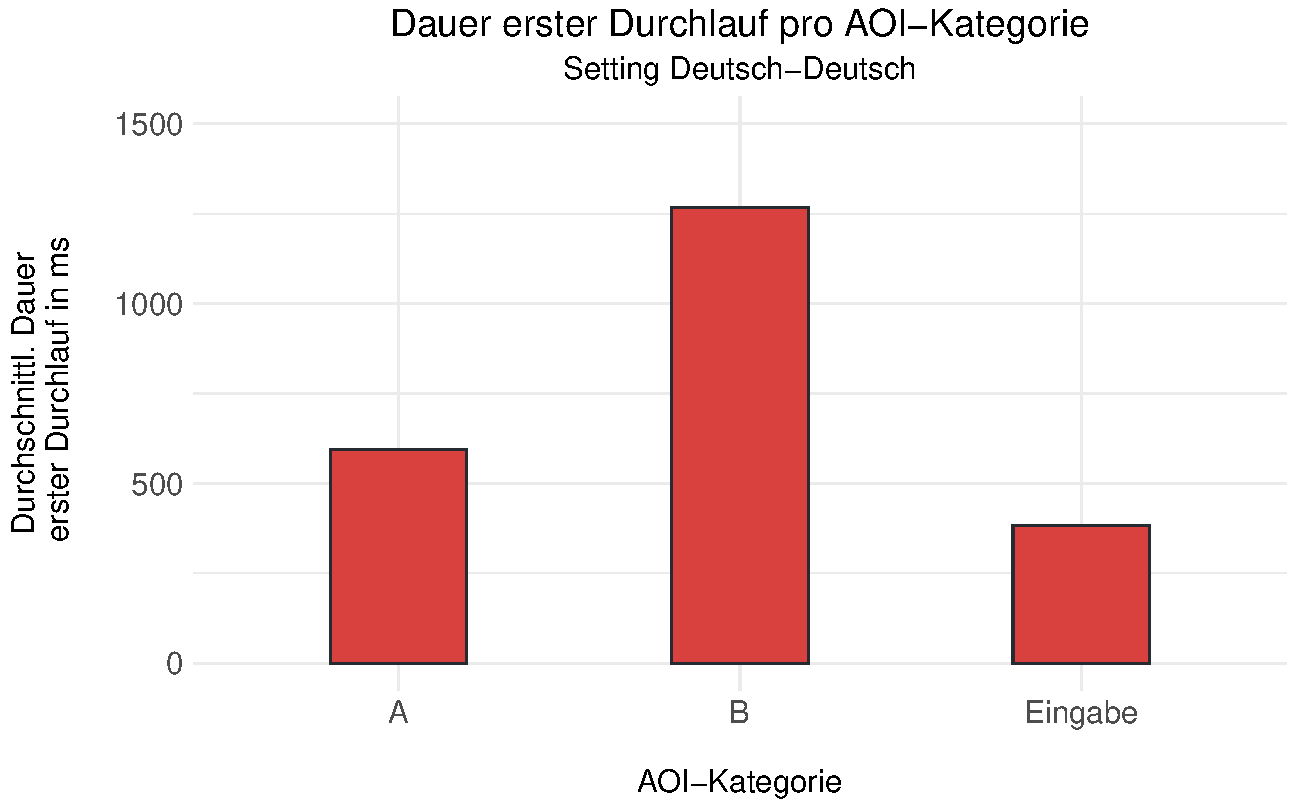
\includegraphics[width=\textwidth]{Figures/EyeTracking/DD/ggplot_DD_meanfrundwell_AOI_de}
	\caption{Durchschnittliche Betrachtungsdauer im ersten Durchlauf pro AOI-Kategorie im Setting Deutsch-Deutsch}
	\label{K6:fig:DeDe:mean-error-FRDwell}
\end{figure}

%------------------------------------------------------------------------

Wie die graphische Inspektion\is{Inspektion!graphische} des Datensatzes anhand von \figref{K6:fig:DD:density-IAFRunD} belegt, kann nicht von einer Normalverteilung ausgegangen werden. Eine logarithmische Transformation\is{Statistik!Transformation!logarithmische} (rechte Seite der Abbildung) ändert nichts an dieser Beobachtung. Auch die statistische Untersuchung des Datensatzes mittels Shapiro-Wilk-Test\is{Shapiro-Wilk-Test}\is{Statistik!Testverfahren!Shapiro-Wilk-Test} lehnt die Annahme einer Normalverteilung ab (roh: $W = 0,67,\allowbreak\ p < 0,001$ und log10: $W = 0,98,\allowbreak\ p < 0,01$).

%------------------------------------------------------------------------

\begin{figure}
    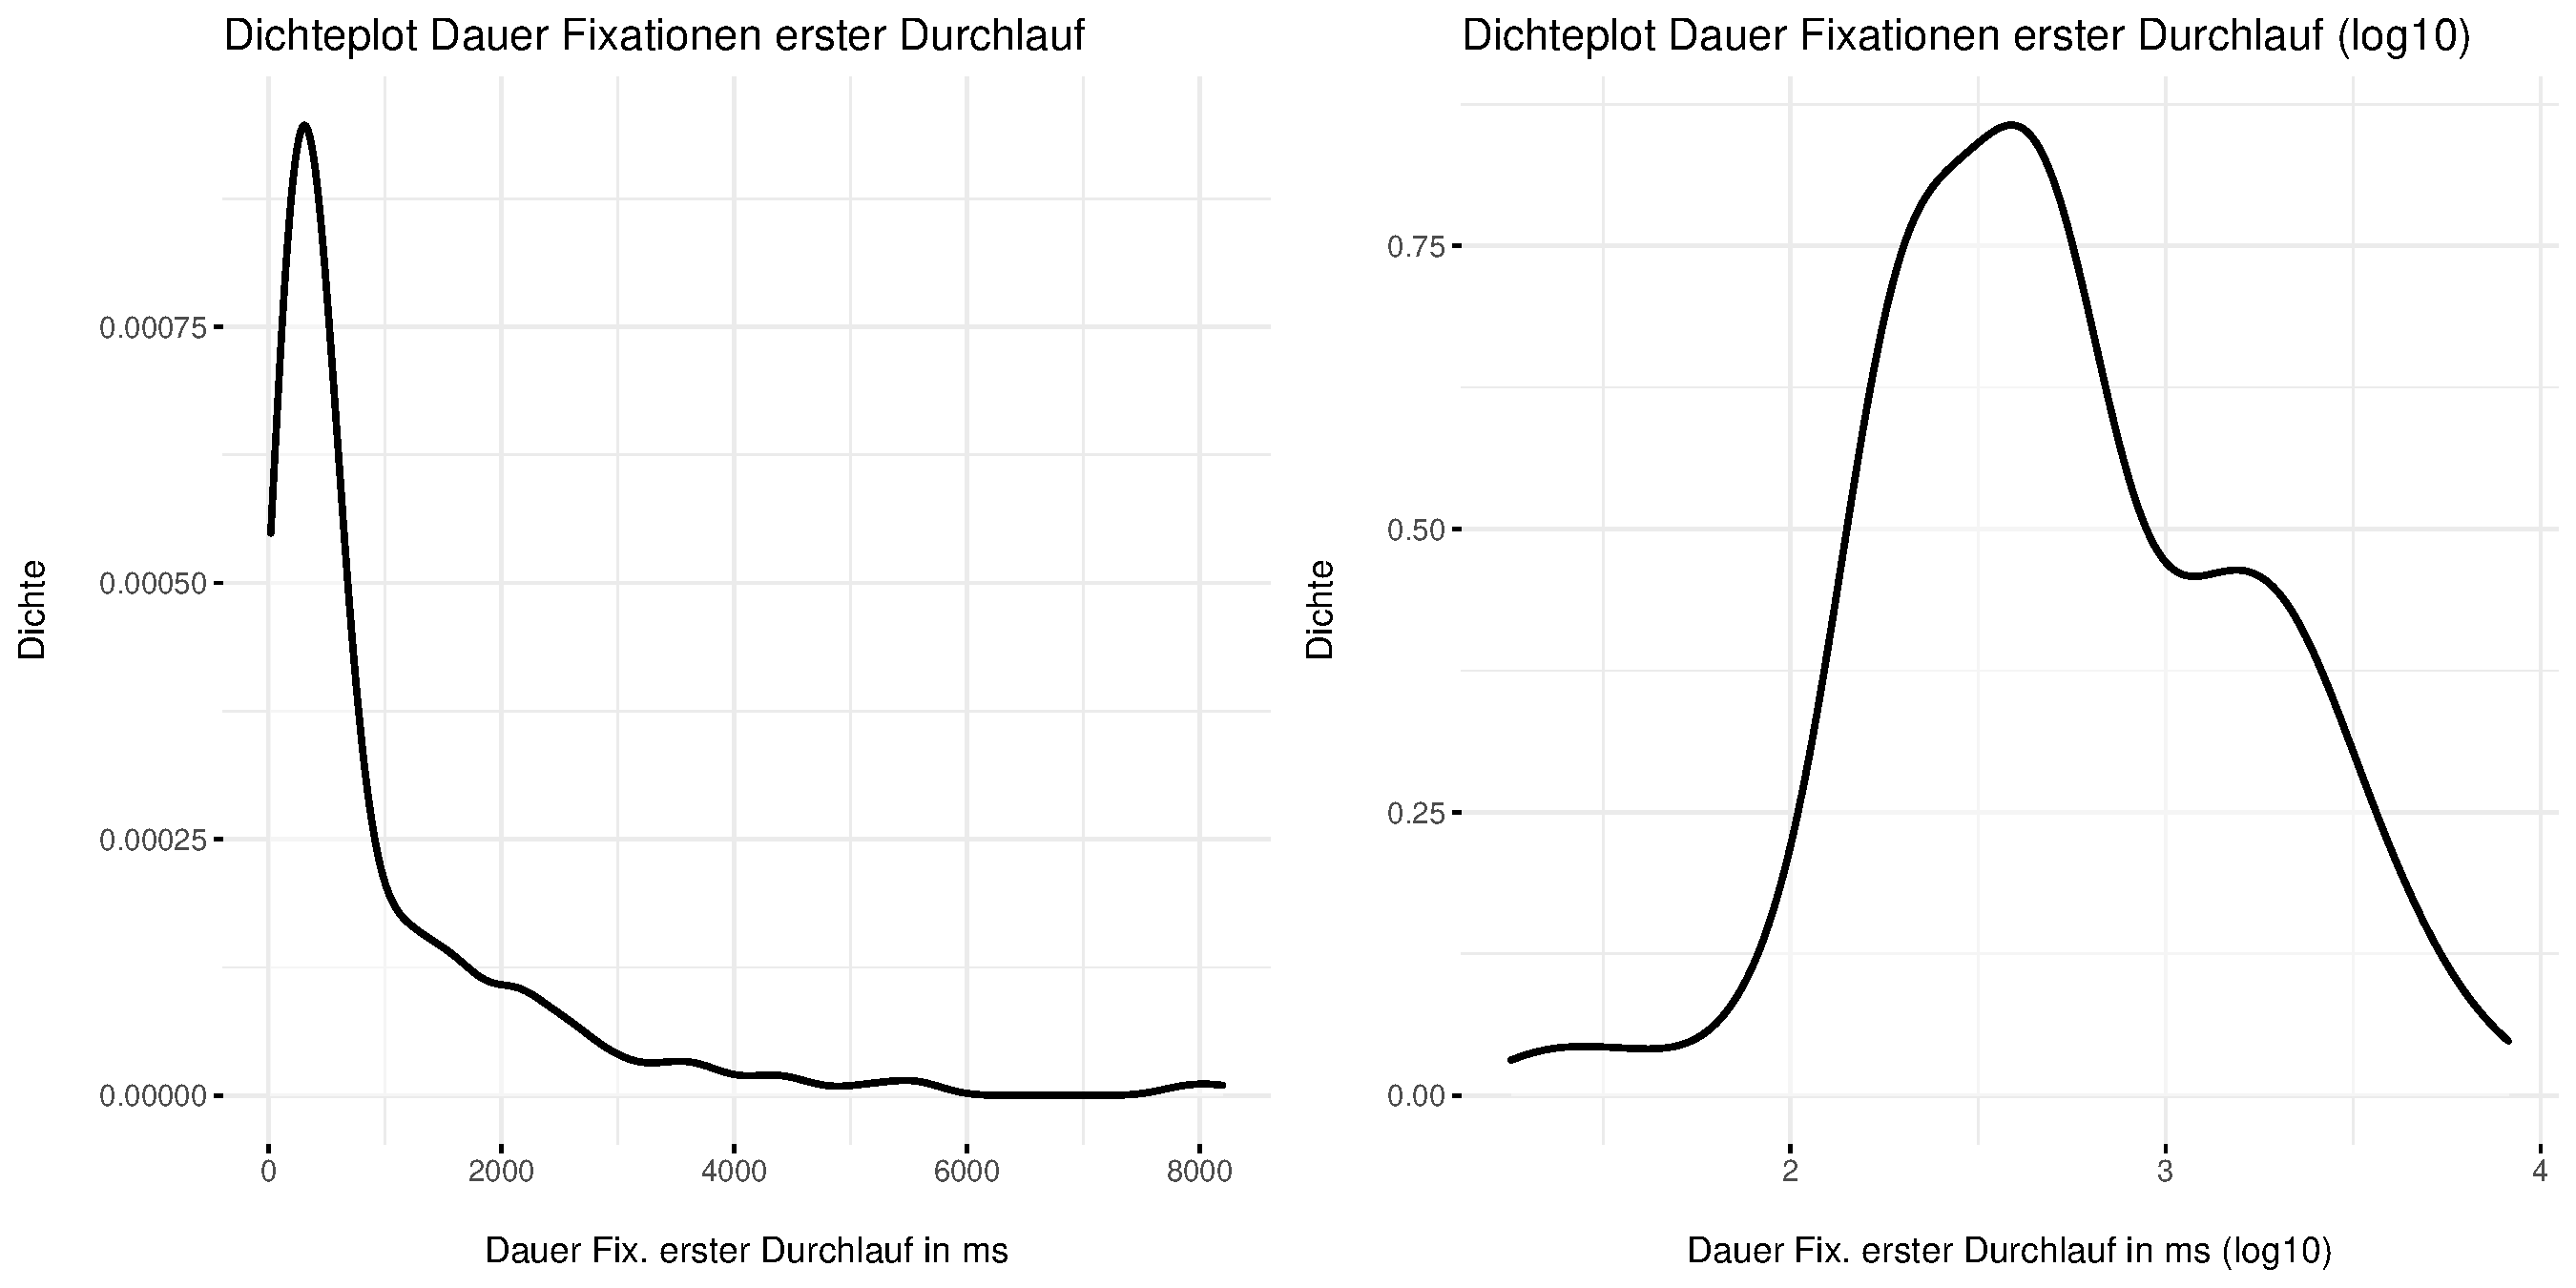
\includegraphics[width=\textwidth]{Figures/EyeTracking/DD/ggplot_DD-IAFRunD_density_de}
	\caption[Verteilung der Dauer der Fixationen im ersten Durchlauf]{Verteilung der Dauer der Fixationen im ersten Durchlauf: normal (links), logarithmisch transformiert (rechts)}
	\label{K6:fig:DD:density-IAFRunD}
\end{figure}

%------------------------------------------------------------------------

Keine Auffälligkeiten werden bei der Betrachtung der Unterschiede in der Dauer des ersten Durchlaufs pro AOI in Verbindung mit den einzelnen Teilnehmer{\textperiodcentered}innen festgestellt. Ein Kruskal-Wallis"=Test ist hierbei nicht signifikant ($\chi^2(6) = 9,73, p = 0,14$). Ein weiterer Kruskal-Wallis-Test\is{Kruskal-Wallis-Test}\is{Statistik!Testverfahren!Kruskal-Wallis-Test} deutet darauf hin, dass Unterschiede bei der Dauer des ersten Durchlaufs pro AOI zwischen den einzelnen AOI-Kategorien bestehen ($\chi^2(2) = 19,08, p < 0,01$). Anschließend durchgeführte Post-hoc-Tests (Dunn-Benjamini-Hochberg-Tests, Tab.\,\ref{K6:tab:DeDe:dunntest-iafrd})\is{Dunn-Benjamini-Hochberg-Test}\is{Statistik!Testverfahren!Dunn-Benjamini-Hochberg-Test} zeigen, dass sich vor allem das Paar \emph{A-B} ($z = -4,19, p < 0,01, r = 0,43$) unterscheidet, sodass gefolgert werden kann, dass die Durchlaufdauer von der AOI-Kategorie, und speziell von der Richtung (hereinkommende Nachrichten), abhängt. Dabei handelt es sich gemäß der Effektstärke nach \citet{cohen_power_1992}\is{Cohen!Effektstärke nach}\is{Statistik!Testverfahren!Effektstärke nach Cohen} um einen mittleren Effekt.\largerpage

%------------------------------------

\begin{table}
    \begin{tabular}{lS[table-format=-1.6]S[table-format=1.4{***}]r}
    \lsptoprule
        {AOI-Kategoriepaar} & {$z$} & \multicolumn{1}{c}{$p$ (angepasst)} & \multicolumn{1}{c}{Effekt}\\ 
        \midrule
        A-B       & -4,188020 & 0,0000{***} & 0,43 \\ 
        A-Eingabe & 0,444057 & 0,3285 & -  \\ 
        B-Eingabe & 1,855061 & 0,0477 & - \\ 
        \lspbottomrule
    \end{tabular}
    \caption{Ergebnisse des Dunn-Tests: Gruppierte Vergleiche der Dauer des ersten Durchlaufs nach AOI-Kategorie\label{K6:tab:DeDe:dunntest-iafrd}}
\end{table}


%------------------------------------

Da die unabhängige Variable der progressiven ersten Fixation\is{Fixation!progressive erste} nur zwei Ausprägungen aufweist, wird der exakte Mann-Whitney"=U-Test\is{Mann-Whitney-U-Test}\is{Statistik!Testverfahren!Mann-Whitney-U-Test} angewendet. Dieses Testverfahren belegt, dass Unterschiede bei der Dauer der ersten Durchläufe pro AOI zwischen beiden Arten der erstmaligen Fixation bestehen ($U = 6.795,5,\allowbreak\ p < 0,05, r = 0,14$). Dabei handelt es sich gemäß der Effektstärke nach \citet{cohen_power_1992}\is{Cohen!Effektstärke nach}\is{Statistik!Testverfahren!Effektstärke nach Cohen} um einen schwachen Effekt.

Noch genauer zeigen sich signifikante Unterschiede bei der Durchlaufdauer der eigenen Chatbeiträge (\emph{A}), wenn zuvor ein AOI mit höherer Ordnungszahl betrachtet wurde, als wenn es sich um eine tatsächliche chronologische erstmalige Fixation handelt. Ein exakter Mann-Whitney"=U"=Test\is{Mann-Whitney-U-Test}\is{Statistik!Testverfahren!Mann-Whitney-U-Test} ($U = 1.342,5, p < 0,05,\allowbreak r = 0,21$) in Verbindung mit einer Untersuchung der Effektstärke nach \citet{cohen_power_1992}\is{Cohen!Effektstärke nach}\is{Statistik!Testverfahren!Effektstärke nach Cohen} zeigt dabei einen schwachen Effekt. Ein Mann-Whitney"=U-Test\is{Mann-Whitney-U-Test}\is{Statistik!Testverfahren!Mann-Whitney-U-Test} für die Betrachtung der progressiven ersten Fixation der fremden Chatbeiträge (\emph{B}) erweist sich als nicht auffällig ($U = 1.976,0, p = 0,251, r = 0,1$).

Die Durchlaufdauer korreliert signifikant mit der Größe der AOI ($r_{s} = 0,28,\allowbreak\ p < 0,01, n = 1.775.506$)\is{Spearman's Rho}\is{Korrelationstest nach Spearman}\is{Statistik!Testverfahren!Korrelationstest nach Spearman}. Dabei handelt es sich nach \citet{cohen_power_1992}\is{Cohen!Effektstärke nach}\is{Statistik!Testverfahren!Effektstärke nach Cohen} um einen schwachen Effekt. Das Bestimmtheitsmaß beträgt 7,59\,\%.
\is{Durchlauf!Dauer des ersten|)}


%------------------------------------------------------------------------

\subsubsection{Gesamtverweildauer}
\label{K6:subsubsec:dwelltime:DD}

%------------------------------------------------------------------------

\is{Verweildauer!Gesamt-|(}
\tabref{K6:tab:DeDe:mean-sd-dwell} gibt Summe, Mittelwert und Standardabweichung der Gesamtverweildauer in Millisekunden pro AOI-Kategorie wieder. Auf den Beiträgen des Gegenübers verweilen die Proband{\textperiodcentered}innen mit 1.187.000\,ms beinahe vier Mal so lang wie auf den eigenen Nachrichten, deren Gesamtdauer 378.000\,ms beträgt. Die Eingabemaske wird mit den Nachrichten des Gegenübers vergleichbar lange fixiert, nämlich 1.089.000\,ms. So ergibt sich in der Summe eine Gesamtdauer von 2.653.000\,ms für alle AOI. Mit Blick auf die Mittelwerte ergibt sich ein ähnliches Bild. Auch hier macht die durchschnittliche Verweildauer\is{Verweildauer!durchschnittliche} für die eigenen Nachrichten (3.000\,ms) etwa ein Drittel der Betrachtungsdauer der Nachrichten des Gegenübers (8.900\,ms) aus.\largerpage

%------------------------------------

\begin{table}
    \begin{tabular}{lrrrr} 
    \lsptoprule
        {AOI-Kategorie} & \multicolumn{1}{c}{Summe} & \multicolumn{1}{c}{Mittelwert} & \multicolumn{1}{c}{Median} & \multicolumn{1}{c}{SD} \\ 
        \midrule
        A & 377.527 & 3.069,33 & 1.330 & 4.908,75 \\ 
        B & 1.186.758  & 8.856,40 & 5.368 & 12.609,55 \\ 
        Eingabe & 1.088.618  & 155.516,86 & 102.914 & 126.036,86 \\ 
        \midrule
        Global & 2.652.903 & 10.048,88 & 3.237 & 32.259,90 \\ 
        \lspbottomrule
    \end{tabular}
    \caption[Summe, Mittelwert, Median und SD der Gesamtverweildauer]
            {Summe, Mittelwert, Median und SD der Gesamtverweildauer 
             pro AOI-Kategorie\label{K6:tab:DeDe:mean-sd-dwell}}
    
\end{table}

\begin{figure}
    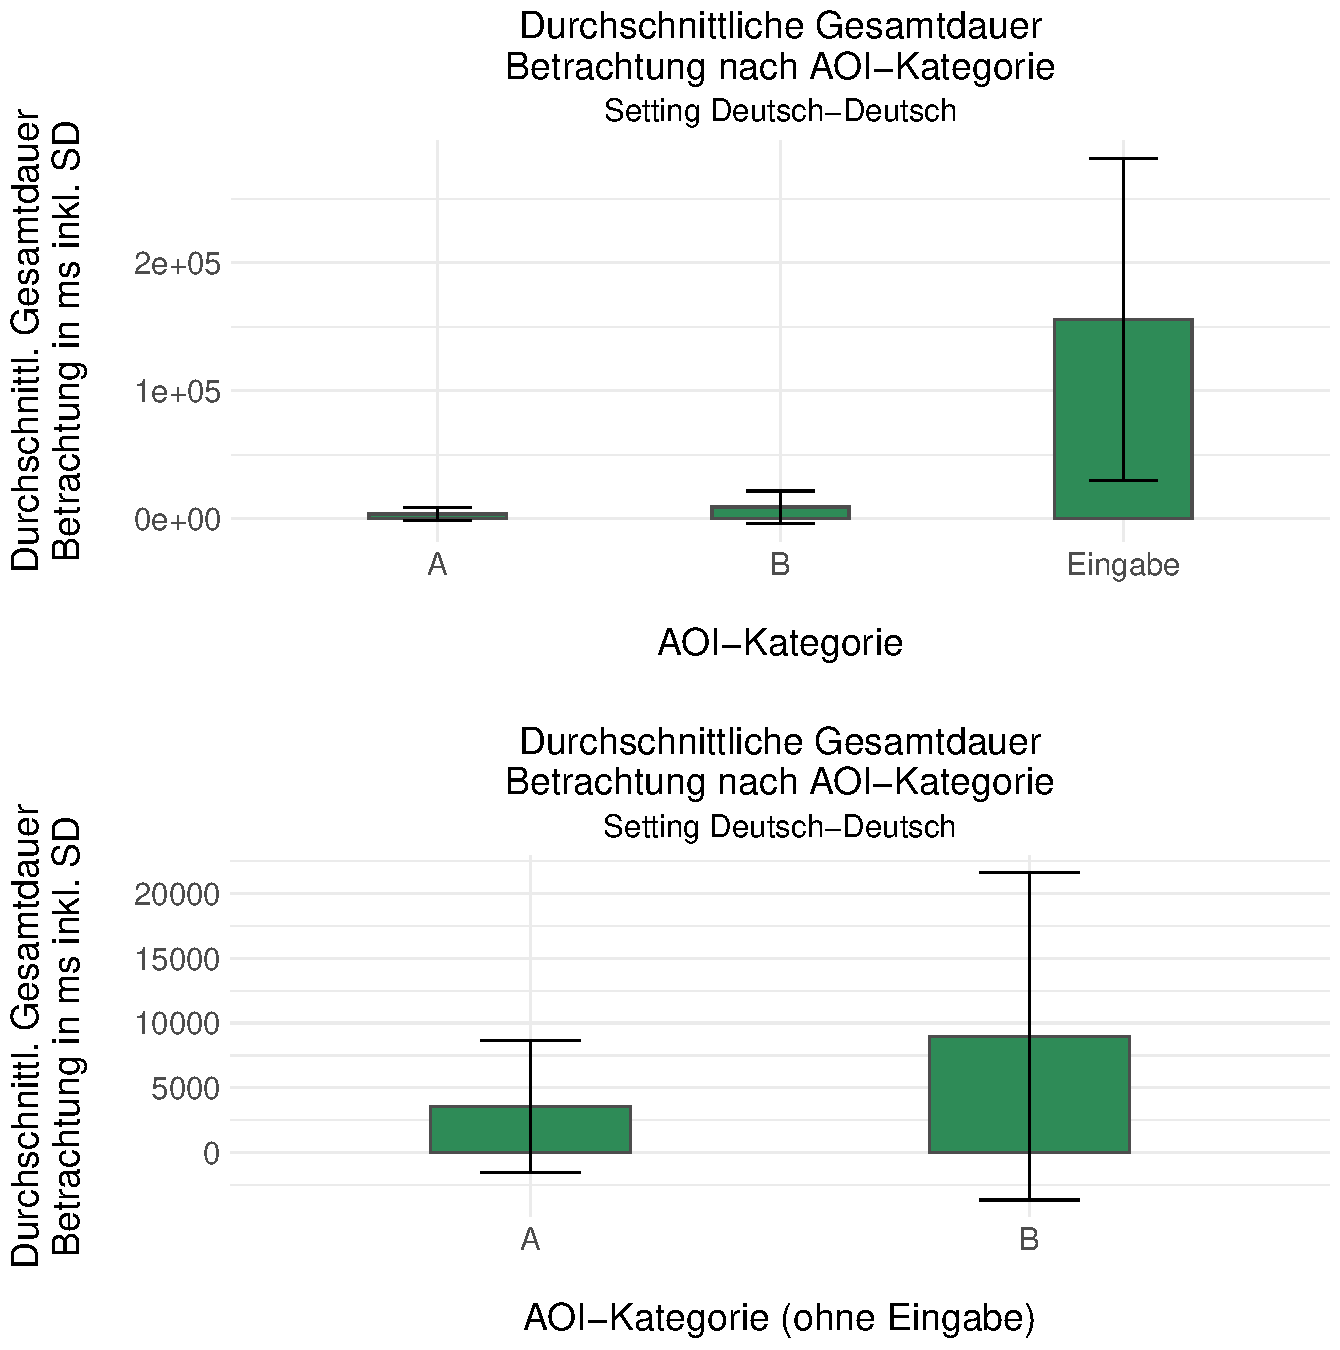
\includegraphics[width=.85\textwidth]{Figures/EyeTracking/DD/ggplot_DD_mean-dwell_AOI-grid-arrange_de}
	\caption{Durchschnittliche Betrachtungsdauer pro AOI-Kategorie im Setting Deutsch-Deutsch, mit (oben) und ohne (unten) Eingabemaske}
	\label{K6:fig:DD:mean-Dwell}
\end{figure}

%------------------------------------------------------------------------

Wie die graphische Inspektion\is{Inspektion!graphische} des Datensatzes anhand von \figref{K6:fig:DD:density-Dwell} belegt, kann nicht von einer Normalverteilung ausgegangen werden. Eine logarithmische Transformation\is{Statistik!Transformation!logarithmische} (rechte Seite der Abbildung) ändert nichts an dieser Beobachtung. Auch die statistische Untersuchung des Datensatzes mittels Shapiro-Wilk-Test\is{Shapiro-Wilk-Test}\is{Statistik!Testverfahren!Shapiro-Wilk-Test} lehnt die Annahme einer Normalverteilung ab (roh: $W = 0,27,\allowbreak\ p < 0,001$ und log10: $W = 0,99, p < 0,001$).

%------------------------------------------------------------------------

\begin{figure}
    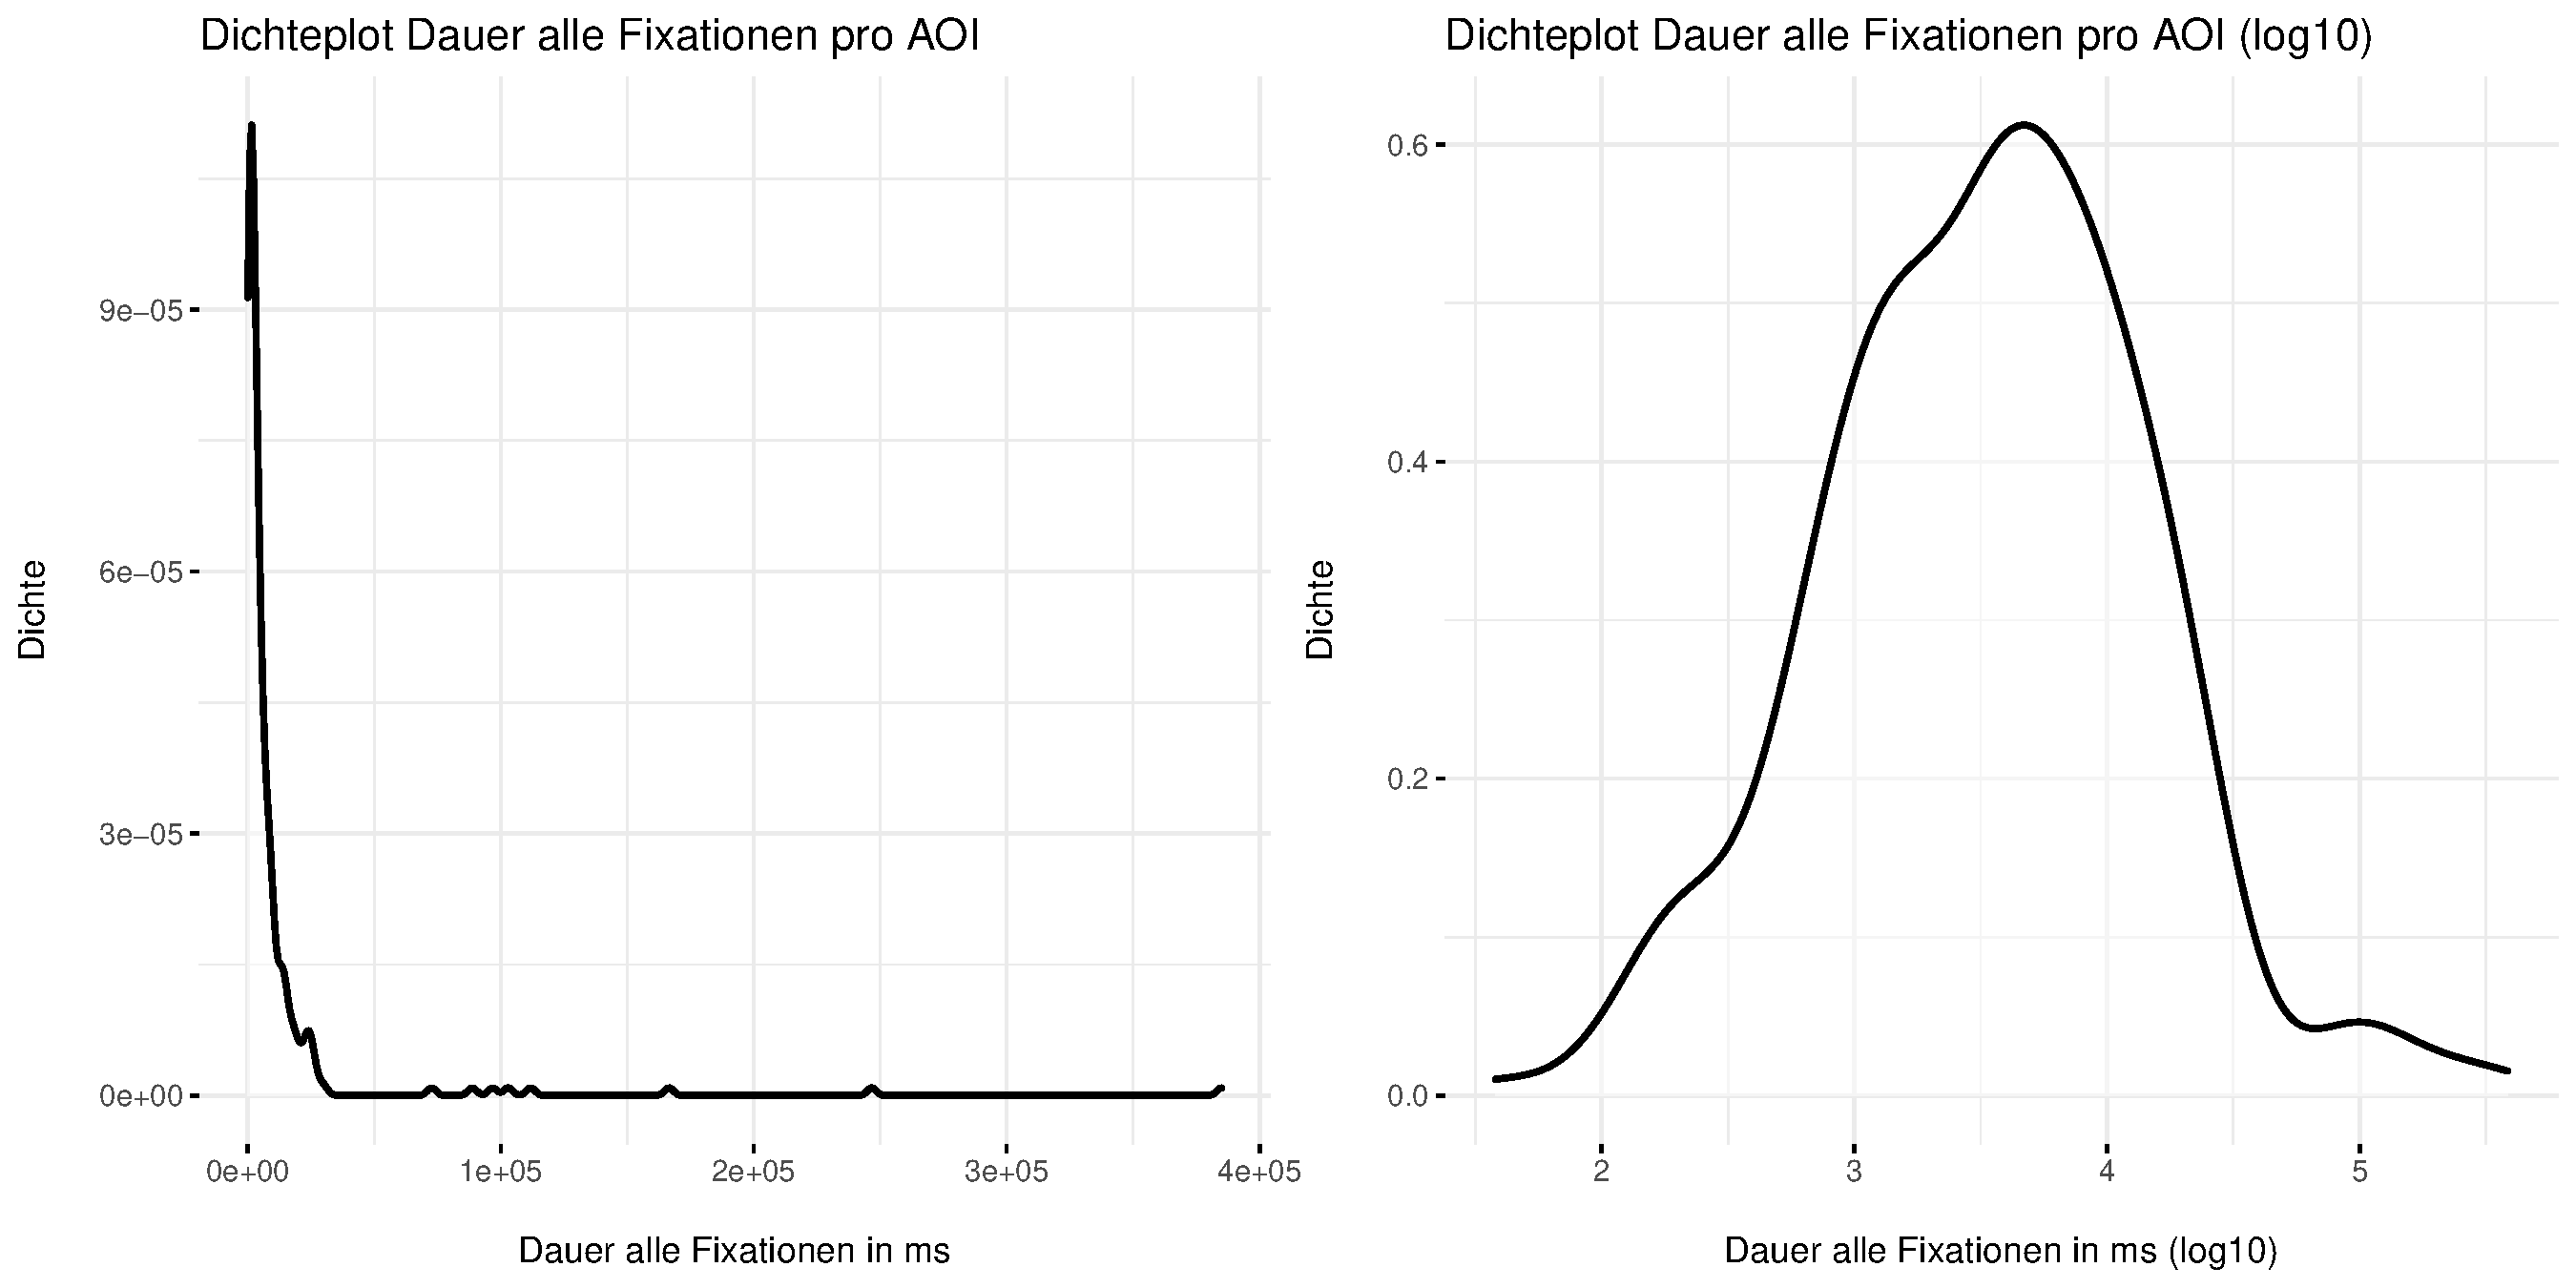
\includegraphics[width=\textwidth]{Figures/EyeTracking/DD/ggplot_DD-Dwell_density_de}
	\caption{Verteilung der Gesamtdauer aller Durchläufe: normal (links), 
             logarithmisch transformiert (rechts)\label{K6:fig:DD:density-Dwell}}
\end{figure}

%------------------------------------------------------------------------

Keine Auffälligkeiten werden bei der Betrachtung der Unterschiede in der Gesamtverweildauer in Verbindung mit den einzelnen Teilnehmer{\textperiodcentered}innen festgestellt. Ein Kruskal-Wallis"=Test ist hierbei nicht signifikant ($\chi^2(6) = 4,66,\allowbreak\ p = 0,59$). Ein weiterer Kruskal-Wallis"=Test\is{Kruskal-Wallis-Test}\is{Statistik!Testverfahren!Kruskal-Wallis-Test} zeigt allerdings, dass Unterschiede in der zentralen Tendenz der Gesamtverweildauer zwischen den einzelnen AOI"=Kategorien bestehen ($\chi^2(2) = 48,55, p < 0,01$). Anschließend durchgeführte Post-hoc"=Tests (Dunn-Benjamini"=Hochberg-Tests, s. \tabref{K6:tab:DeDe:dunntest-dwell})\is{Dunn-Benjamini-Hochberg-Test}\is{Statistik!Testverfahren!Dunn-Benjamini-Hochberg-Test} zeigen, dass sich alle drei möglichen Gruppierungen signifikant unterscheiden, sodass gefolgert werden kann, dass die Verweildauer\is{Durchlauf!-dauer} von der AOI-Kategorie abhängt. Unter Anwendung der Effektstärke nach \citet{cohen_power_1992}\is{Cohen!Effektstärke nach}\is{Statistik!Testverfahren!Effektstärke nach Cohen} handelt es sich bei \emph{B-Eingabe} um einen schwachen Effekte ($r = 0,22$), bei \emph{A-B} und \emph{A-Eingabe} um jeweils mittlere Effekte ($r = 0,45$ und $r = 0,46$).

%------------------------------------

\vfill
\begin{table}[H]
    \begin{tabular}{lclc}  
    \lsptoprule
        {1}{c}{AOI-Kategoriepaar} & \multicolumn{1}{c}{$z$} & \multicolumn{1}{c}{$p$ (angepasst)} & {Effekt} \\
        \midrule
        A-B       & −6,920374 & 0,0000 *** & 0,45 \\ 
        A-Eingabe & −4,867397 & 0,0000 *** & 0,46 \\ 
        B-Eingabe & −2,649329 & 0,0040 ** & 0,22 \\ 
        \lspbottomrule
    \end{tabular}
    \caption{Ergebnisse des Dunn-Tests: Gruppierte Vergleiche der Gesamtverweildauer nach AOI-Kategorie}
    \label{K6:tab:DeDe:dunntest-dwell}
\end{table}
\vfill\pagebreak

%------------------------------------

Zur Untersuchung der progressiven ersten Fixation\is{Fixation!progressive erste} wird der exakte Mann-Whitney"=U-Test\is{Mann-Whitney-U-Test}\is{Statistik!Testverfahren!Mann-Whitney-U-Test} angewendet. Dieses Testverfahren belegt, dass Unterschiede bei der Gesamtverweildauer pro AOI zwischen beiden Arten der erstmaligen Fixation bestehen ($U = 6.298,0, p < 0,001, r = 0,21$). Dabei handelt es sich gemäß der Effektstärke nach \citet{cohen_power_1992}\is{Cohen!Effektstärke nach}\is{Statistik!Testverfahren!Effektstärke nach Cohen} um einen schwachen Effekt. Ebenfalls zeigen sich signifikante Unterschiede bei der Verweildauer der Chatbeiträge des Gegenübers (\emph{B}), wenn zuvor ein AOI mit höherer Ordnungszahl betrachtet wurde, als wenn es sich um eine tatsächliche chronologische erstmalige Fixation handelt. Ein exakter Mann-Whitney"=U"=Test\is{Mann-Whitney-U-Test}\is{Statistik!Testverfahren!Mann-Whitney-U-Test} ($U = 1.796,0, p < 0,05, r = 0,18$) in Verbindung mit einer Untersuchung der Effektstärke nach \citet{cohen_power_1992}\is{Cohen!Effektstärke nach}\is{Statistik!Testverfahren!Effektstärke nach Cohen} zeigt dabei einen schwachen Effekt. Ein Mann-Whitney"=U-Test\is{Mann-Whitney-U-Test}\is{Statistik!Testverfahren!Mann-Whitney-U-Test} für die Betrachtung der progressiven ersten Fixation der eigenen Chatbeiträge (\emph{A}) liegt auf der Grenze des Signifikanzniveaus ($U = 1.378,0, p = 0,051, r = 0,19$).

Die Gesamtverweildauer\is{Fixation!-sdauer} korreliert signifikant mit der Größe der AOI\is{Area of Interest!Größe des} ($r_{s} = 0,75, p < 0,01, n = 764.790$). Dabei handelt es sich nach \citet{cohen_power_1992}\is{Cohen!Effektstärke nach}\is{Statistik!Testverfahren!Effektstärke nach Cohen} um einen starken Effekt. Das Bestimmtheitsmaß beträgt 56,34\,\%.
\is{Verweildauer!Gesamt-|)}


%------------------------------------------------------------------------

\subsubsection{Regressive Durchlaufdauer}
\label{K6:subsubsec:regpd:DD}

%------------------------------------------------------------------------

\is{Durchlauf!-dauer!regressive|(}\is{regressive Durchlaufdauer}
\begin{sloppypar}
\tabref{K6:tab:DeDe:mean-sd-iaregpd} stellt Summe, Mittelwert und Standardabweichung der regressiven Durchlaufdauer in Millisekunden pro AOI-Kategorie dar. Der Gesamtwert beträgt 2.848.000\,ms. Die Nachrichten der Proband{\textperiodcentered}innen werden insgesamt 1.173.000\,ms betrachtet, wohingegen die Gesamtdauer der regressiven Durchlaufdauer der Beiträge des Gegenübers nur 1.093.330\,ms beträgt. Die Mittelwerte betragen jeweils 11.067\,ms (\emph{A}) und 8.282\,ms (\emph{B}).
\end{sloppypar}

%------------------------------------
\vfill
\begin{table}[H]
    \begin{tabular}{lrrrr}
    \lsptoprule
        {AOI-Kategorie} & \multicolumn{1}{c}{Summe} & \multicolumn{1}{c}{Mittelwert} & \multicolumn{1}{c}{Median} &\multicolumn{1}{c}{SD} \\ 
        \midrule
        A   & 1.173.109 & 11.067,07 & 4.460,5 & 16.635,21 \\ 
        B   & 1.093.330 & 8.282,80 & 5.061,5 & 10.272,36 \\ 
        Eingabe   & 581.094 & 83.013,43 & 1.678,0 &  212.477,43 \\ 
        \midrule
        Global  & 2.847.533 & 11.622,58 & 4.797,0 & 37.924,73 \\ 
        \lspbottomrule
    \end{tabular}
    \caption[Summe, Mittelwert, Median und SD der regressiven Durchlaufdauer]
            {Summe, Mittelwert, Median und SD der regressiven Durchlaufdauer 
             in ms pro AOI-Kategorie\label{K6:tab:DeDe:mean-sd-iaregpd}}
\end{table}
\vfill\pagebreak

%------------------------------------

Wie auch schon im anderen Setting erklärt, wurde die Eingabemaske als statisches AOI\is{Area of Interest!statisches} annotiert. Der hohe Mittelwert erklärt sich daher möglicherweise aus dem anfänglichen Warteverhalten der Versuchspersonen bis die Gesprächspartner{\textperiodcentered}innen die erste Nachricht gesendet hat. Bis zu diesem Zeitpunkt verweilten die Proband{\textperiodcentered}innen meist sehr lange auf der Eingabemaske und damit innerhalb des AOI. Wie die graphische Inspektion\is{Inspektion!graphische} des Datensatzes anhand von \figref{K6:fig:DeDe:density-iaregpd} belegt, kann nicht von einer Normalverteilung ausgegangen werden. Eine logarithmische Transformation\is{Statistik!Transformation!logarithmische} (rechte Seite der Abbildung) ändert nichts an dieser Beobachtung. Die statistische Untersuchung des Datensatzes mittels Shapiro-Wilk"=Test\is{Shapiro-Wilk-Test}\is{Statistik!Testverfahren!Shapiro-Wilk-Test} lehnt die Annahme einer Normalverteilung ab (roh: $W = 0,21, p < 0,001$ bzw. log10: $W = 0,99, p < 0,05$). Daher wird mit nicht-parametrischen Tests\is{Statistik!Testverfahren!nicht-parametrisches} gearbeitet.

%------------------------------------------------------------------------

\begin{figure}
    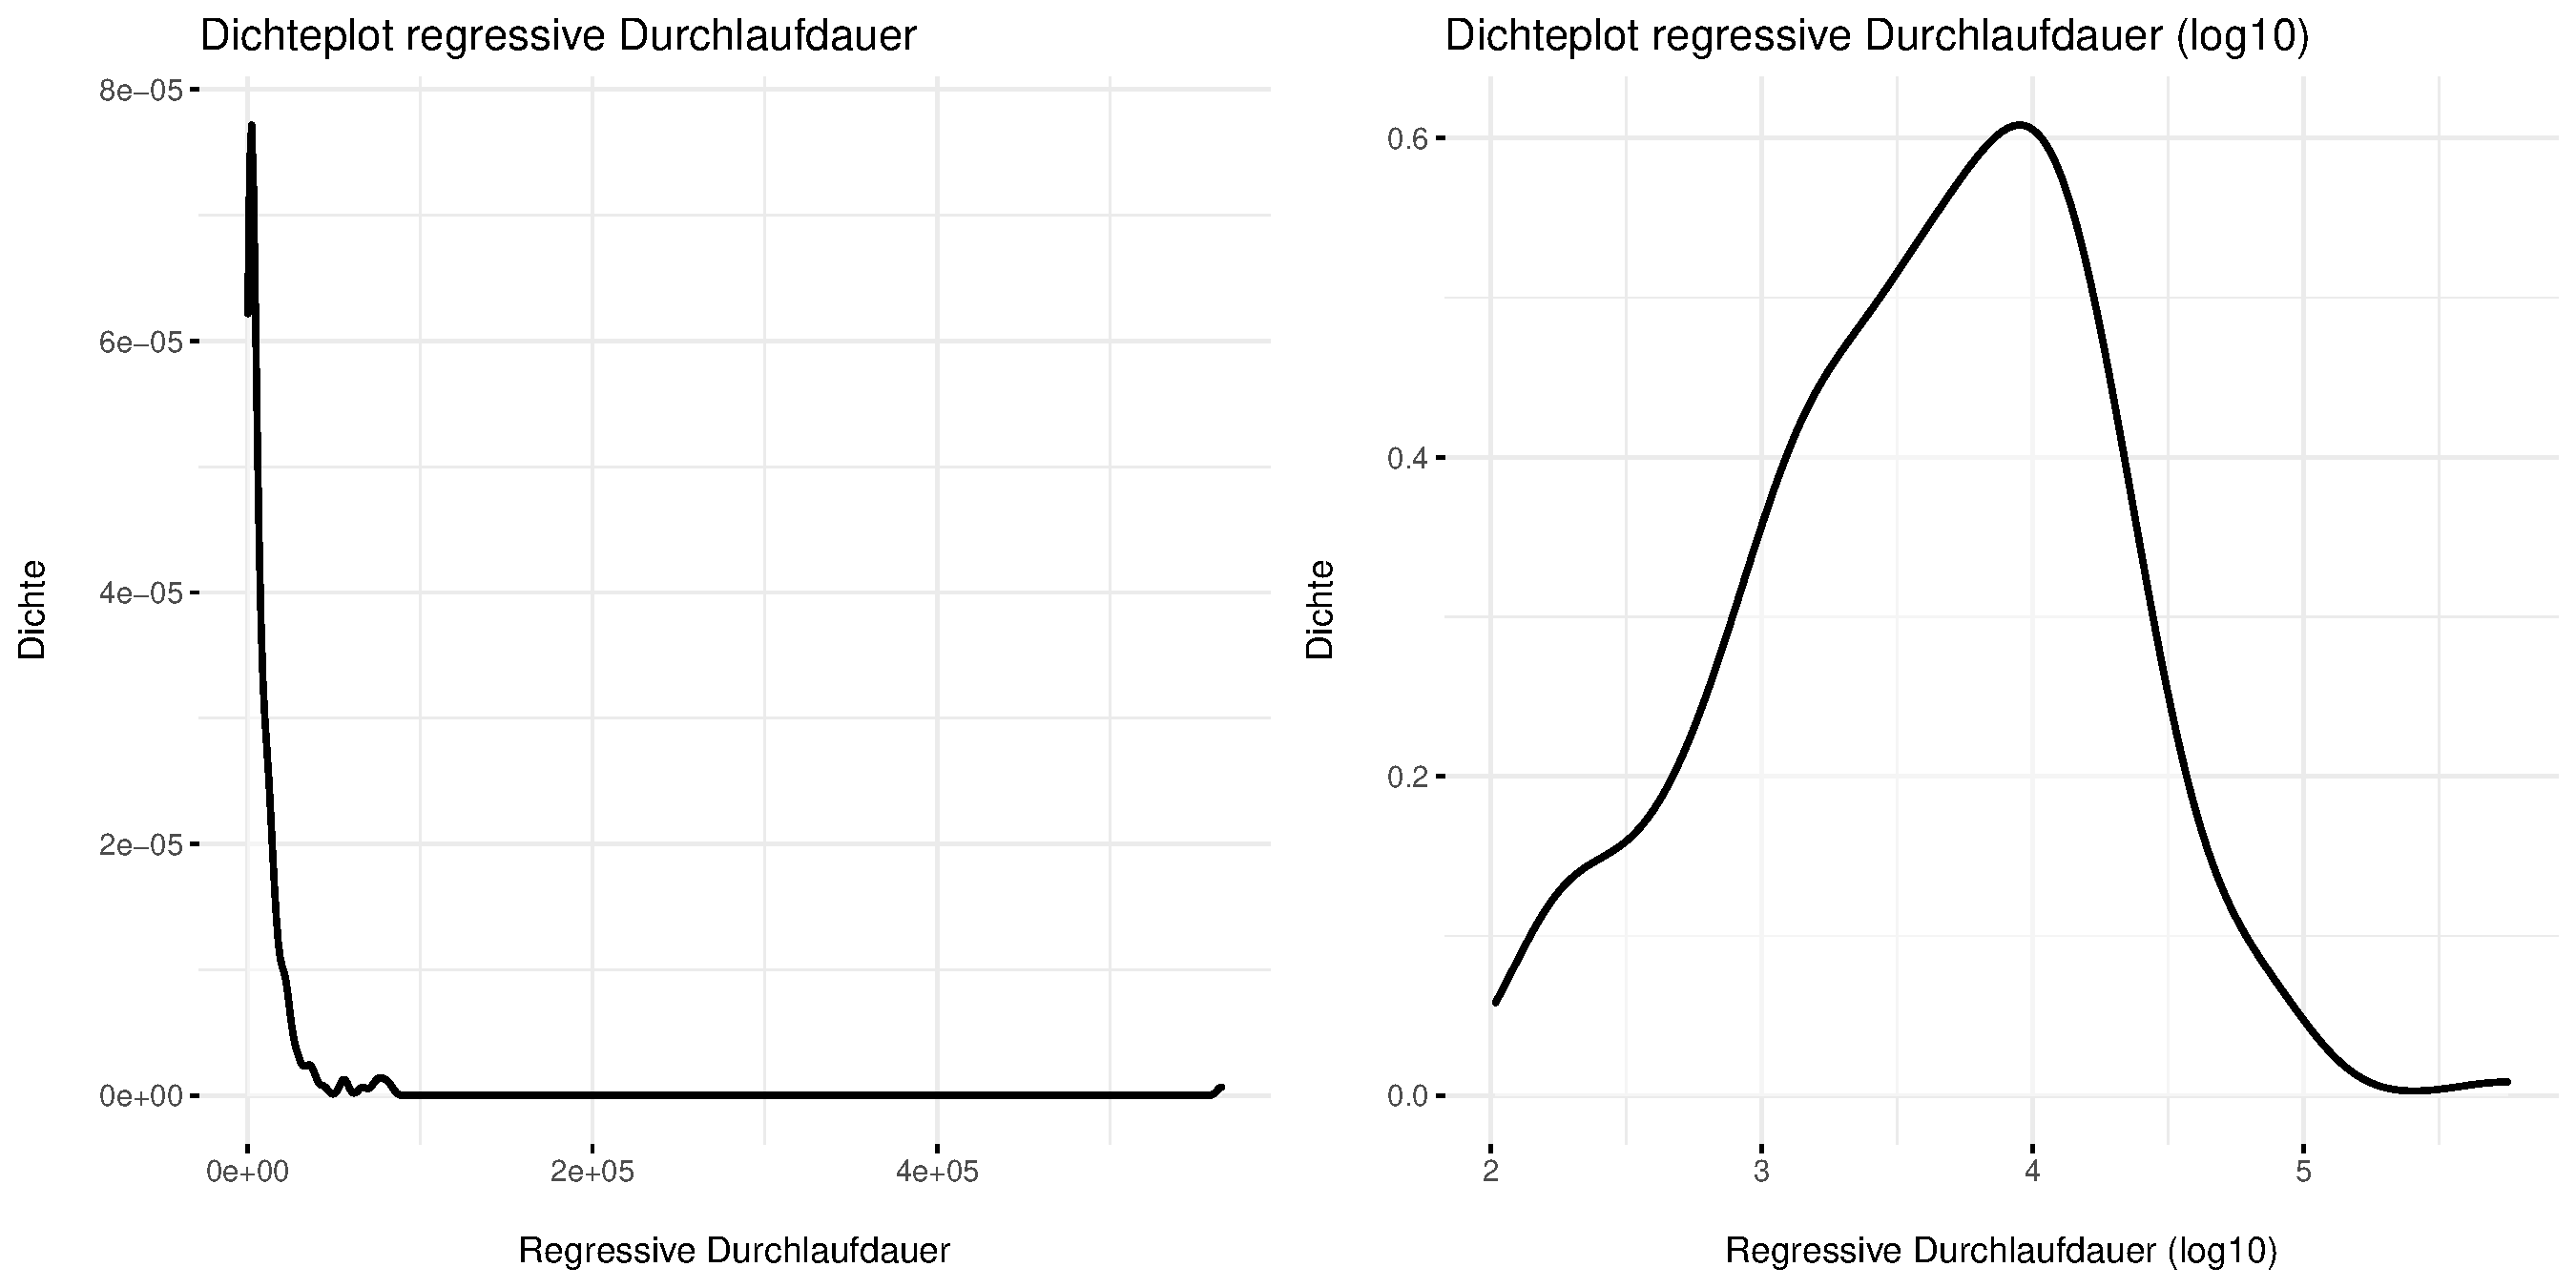
\includegraphics[width=\textwidth]{Figures/EyeTracking/DD/ggplot_DD-RegPD_density_de}
	\caption{Verteilung der regressiven Durchlaufdauer: normal (links), logarithmisch transformiert (rechts)}
	\label{K6:fig:DeDe:density-iaregpd}
\end{figure}

%------------------------------------------------------------------------

\begin{sloppypar}
Ein Kruskal-Wallis"=Test\is{Kruskal-Wallis-Test}\is{Statistik!Testverfahren!Kruskal-Wallis-Test} deutet darauf hin, dass Unterschiede bei der regressiven Durchlaufdauer zwischen den einzelnen Teilnehmer{\textperiodcentered}innen bestehen ($\chi^2(6) = 33,54,\allowbreak\ p < 0,001$). Ein zweiter Kruskal-Wallis"=Test\is{Kruskal-Wallis-Test}\is{Statistik!Testverfahren!Kruskal-Wallis-Test} belegt, dass keine Unterschiede bei der regressiven Durchlaufdauer zwischen den einzelnen AOI-Kategorien bestehen ($\chi^2(2) = 0,9, p = 0,64$).
\end{sloppypar}

Es besteht wiederum ein signifikanter Unterschied bei der regressiven Durchlaufdauer zwischen AOI, die in chronologischer Reihenfolge betreten wurden und jenen, die aus einem AOI mit höherer Ordnungszahl besucht wurden. Da die Variable der progressiven ersten Fixation\is{Fixation!progressive erste} nur in zwei Ausprägungen vorliegt, wurde hier der Mann-Whitney"=U-Test\is{Mann-Whitney-U-Test}\is{Statistik!Testverfahren!Mann-Whitney-U-Test} angewendet ($U = 3.899,5,\allowbreak\ p < 0,001,\allowbreak r = 0,52$). Dieser Befund gilt ebenfalls für die Unterteilung nach AOI-Kategorie (\emph{A}: $U = 743,0, p < 0,001, r = 0,62$, \emph{B}: $U = 1.177,0, p < 0,001, r = 0,47$). Für die Durchlaufdauer durch beide Nachrichtenarten macht es demnach einen Unterschied, ob die Proband{\textperiodcentered}innen vorher bereits nachfolgende Nachrichten(-AOI) betrachtet haben oder nicht.

Die regressive Durchlaufdauer korreliert außerdem mit der Größe der AOI\is{Area of Interest!Größe des} ($r_{s} = 0,35, p < 0,01, n = 1.593.303$)\is{Spearman's Rho}\is{Korrelationstest nach Spearman}\is{Statistik!Testverfahren!Korrelationstest nach Spearman}. Dabei handelt es sich nach \citet{cohen_power_1992}\is{Cohen!Effektstärke nach}\is{Statistik!Testverfahren!Effektstärke nach Cohen} um einen mittleren Effekt. Das Bestimmtheitsmaß beträgt 12,24\,\%.
\is{Durchlauf!-dauer!regressive|)}

%------------------------------------
\subsubsection{Selektive Regressive Durchlaufdauer}
\label{K6:para:DeDe:iaselregpd}
%------------------------------------

\is{Durchlauf!-dauer!selektive regressive|(}\is{selektive regressive Durchlaufdauer}
\begin{sloppypar}
\tabref{K6:tab:DeDe:mean-sd-iaselregpd} stellt Summe, Mittelwert und Standardabweichung der regressiven Durchlaufdauer in Millisekunden pro AOI-Kategorie dar. Der Gesamtwert beträgt 1.281.202\,ms. Die Nachrichten der Versuchspersonen werden insgesamt 247.249\,ms betrachtet, wohingegen die Gesamtdauer der regressiven Durchlaufdauer der Beiträge des Gegenübers 632.744\,ms beträgt. Die Mittelwerte betragen jeweils 2.332,54\,ms (\emph{A}) und 4.793,52\,ms (\emph{B}). Die Annotation der Eingabemaske als statisches AOI und die damit verbundenen Konsequenzen für die Auswertung wurden bereits mehrfach erklärt (s.\,o.).
\end{sloppypar}

%------------------------------------



\begin{table}
    \begin{tabular}{lrrrr}
    \lsptoprule
        {AOI-Kategorie} & \multicolumn{1}{c}{Summe} & \multicolumn{1}{c}{Mittelwert} & \multicolumn{1}{c}{Median} &\multicolumn{1}{c}{SD} \\ 
        \midrule
        A &   247.249 &  2.332,54   &   994,0 &  3.883,06 \\
        B &   632.744 &  4.793,52 &  2.600,5  & 7.454,11 \\
        Eingabe  &  401.209 & 57.315,57   & 1.678,0 & 144.493,5 \\ 
        \midrule
        Global &  1.281.202  & 5.229,4 &  1.509,0 &  25.125,72 \\
        \lspbottomrule
    \end{tabular}
    \caption[Summe, Mittelwert, Median und SD der selektiven regressiven Durchlaufdauer]{Summe, Mittelwert, Median und SD der selektiven regressiven Durchlaufdauer in ms pro AOI-Kategorie}
    \label{K6:tab:DeDe:mean-sd-iaselregpd}
\end{table}

%------------------------------------


Wie die graphische Inspektion\is{Inspektion!graphische} des Datensatzes anhand von \figref{K6:fig:DeDe:density-iaselregpd} belegt, kann nicht von einer Normalverteilung ausgegangen werden. Eine logarithmische Transformation\is{Statistik!Transformation!logarithmische} (rechte Seite der Abbildung) ändert nichts an dieser Beobachtung. Die statistische Untersuchung des Datensatzes mittels Shapiro-Wilk"=Test\is{Shapiro-Wilk-Test}\is{Statistik!Testverfahren!Shapiro-Wilk-Test} lehnt die Annahme einer Normalverteilung ab (roh: $W = 0,13, p < 0,001$ bzw. log10: $W = 0,99, p < 0,05$). Daher wird mit nicht-parametrischen Tests\is{nicht-parametrischer Test}\is{Statistik!Testverfahren!nicht-parametrisches} gearbeitet.

%------------------------------------------------------------------------

\begin{figure}
    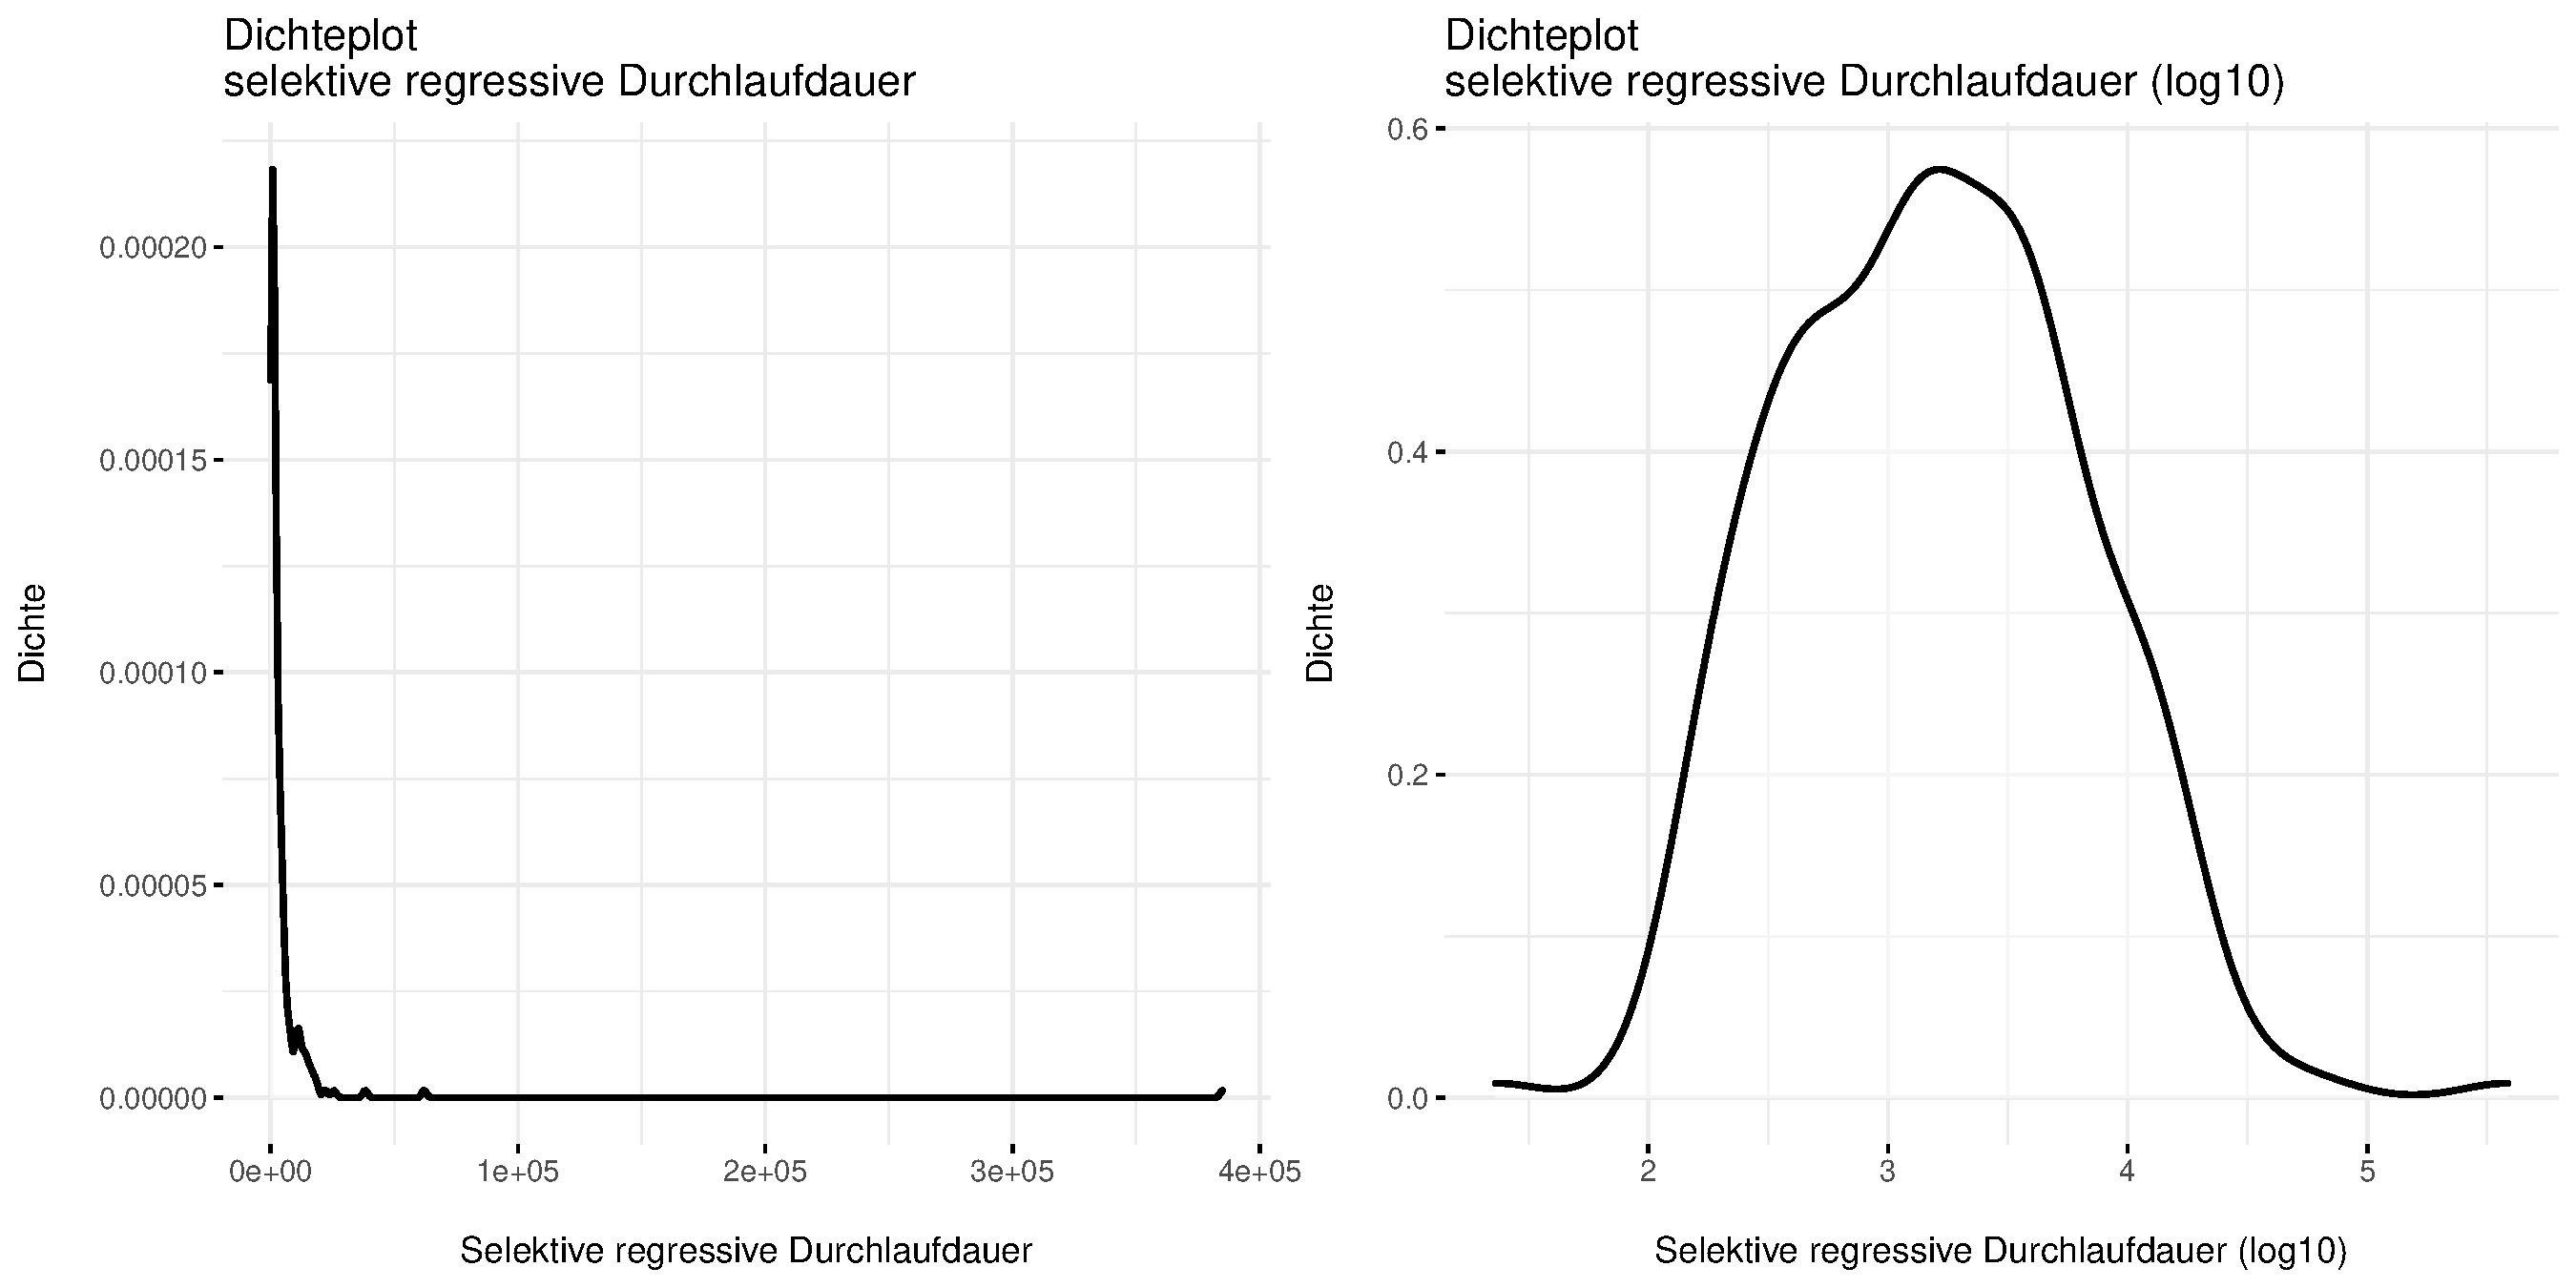
\includegraphics[width=\textwidth]{Figures/EyeTracking/DD/ggplot_DD-SELECT-RegPD_density_de}
	\caption[Verteilung der selektiven regressiven Durchlaufdauer]
            {Verteilung der selektiven regressiven Durchlaufdauer: normal 
             (links), logarithmisch transformiert (rechts)\label{K6:fig:DeDe:density-iaselregpd}}
\end{figure}

%------------------------------------------------------------------------

Ein Kruskal-Wallis"=Test\is{Kruskal-Wallis-Test}\is{Statistik!Testverfahren!Kruskal-Wallis-Test} deutet darauf hin, dass Unterschiede bei der selektiven regressiven Durchlaufdauer zwischen den einzelnen Teilnehmer{\textperiodcentered}innen bestehen ($\chi^2(6) = 15,99, p < 0,01$). Ein zweiter Kruskal-Wallis"=Test\is{Kruskal-Wallis-Test}\is{Statistik!Testverfahren!Kruskal-Wallis-Test} belegt, dass Unterschiede bei der selektiven regressiven Durchlaufdauer zwischen den AOI"=Kategorien bestehen ($\chi^2(2) = 18,36, p < 0,001$). Anschließend durchgeführte Post-hoc"=Tests (Dunn-Benjamini-Hochberg-Tests, s. \tabref{K6:tab:DeDe:dunntest-pupilsize}, S.\,\pageref{K6:tab:DeDe:dunntest-pupilsize})\is{Dunn-Benjamini-Hochberg-Test}\is{Statistik!Testverfahren!Dunn-Benjamini-Hochberg-Test} zeigen, dass sich das Paar \emph{A-B} signifikant unterscheidet. Die Effekstärke ist mit 0,25 allerdings als schwach anzusehen.\largerpage[2]

%------------------------------------

\begin{table}
    \begin{tabular}{lS[table-format=-1.6]S[table-format=1.4{***}]c}  
    \lsptoprule
        {AOI-Kategoriepaar} & {$z$} & {$p$ (angepasst)} & {Effekt} \\
        \midrule
        A-B       & -4,166639 & 0,0000{***} & 0,25 \\ 
        A-Eingabe & -1,756923 & 0,0593 & - \\ 
        B-Eingabe & -0,365754 & 0,3573  & - \\ 
        \lspbottomrule
    \end{tabular}
    \caption{Ergebnisse des Dunn-Tests: Gruppierte Vergleiche der selektiven regressiven Durchlaufdauer nach AOI-Kategorie}
    \label{K6:tab:DeDe:dunntest-iaselregpd}
\end{table}

%------------------------------------

Es besteht wiederum ein signifikanter Unterschied bei der selektiven regressiven Durchlaufdauer zwischen AOI, die in chronologischer Reihenfolge betreten wurden und jenen, die aus einem AOI mit höherer Ordnungszahl besucht wurden (progressive erste Fixation). Hierzu wurde der Mann-Whitney"=U-Test\is{Mann-Whitney-U-Test}\is{Statistik!Testverfahren!Mann-Whitney-U-Test} angewendet ($U = 5.115,0, p < 0,001, r = 0,36$). Dieser Befund gilt ebenfalls für die Unterteilung nach AOI"=Kategorie (\emph{A}: $U = 967,0, p < 0,001, r = 0,47$, \emph{B}: $U = 1.536,5, p < 0,001, r = 0,30$). Für die Durchlaufdauer durch beide Nachrichtenarten macht es demnach einen Unterschied, ob die Proband{\textperiodcentered}innen vorher bereits nachfolgende Nachrichten(-AOI) betrachtet haben oder nicht.

Die selektive regressive Durchlaufdauer korreliert außerdem mit der Größe der AOI\is{Area of Interest!Größe des} ($r_{s} = 0,56, p < 0,01, n = 1.072.123$)\is{Spearman's Rho}\is{Korrelationstest nach Spearman}\is{Statistik!Testverfahren!Korrelationstest nach Spearman}. Dabei handelt es sich nach \citet{cohen_power_1992}\is{Cohen!Effektstärke nach}\is{Statistik!Testverfahren!Effektstärke nach Cohen} um einen starken Effekt. Das Bestimmtheitsmaß beträgt 31,64\,\%.
\is{Durchlauf!-dauer!selektive regressive|)}

%------------------------------------------------------------------------

\subsubsection{Pupillengröße}
\label{K6:subsubsec:dede:psize}\largerpage


%------------------------------------------------------------------------

\is{Pupillengröße|(}
\tabref{K6:tab:DeDe:mean-sd-psize} (S.\,\pageref{K6:tab:DeDe:mean-sd-psize}) zeigt die durchschnittliche Pupillengröße sowie die Standardabweichungen. Bei der Betrachtung der Eingabemaske liegt die Pupillengröße 122 Einheiten (126\,\%) über dem Gesamtschnitt. Die Pupillenweitung bei Betrachtung der Chatbeiträge\is{Chat!-beitrag} des Gegenübers gleicht beinahe dem Durchschnitt (\emph{B}: 473 Einheiten, Durchschnitt 470 Einheiten). Die Pupillengröße beim eigenen Beitrag ist 2,4\,\% kleiner als der Durchschnitt (\emph{A}: 459 Einheiten, Durchschnitt: 470 Einheiten). Der Unterschied zwischen beiden Gruppen (\emph{A}: 459, \emph{B}: 473) beträgt 2,96\,\%.


%------------------------------------

\begin{table}
    \begin{tabular}{lccc} 
    \lsptoprule
        \multicolumn{1}{c}{AOI-Kategorie} & \multicolumn{1}{c}{Mittelwert} & \multicolumn{1}{c}{Median} & \multicolumn{1}{c}{SD} \\ 
        \midrule
        A   & 459,19 & 420,57 & 121,15 \\ 
        B   & 473,07 & 439,29 & 112,05 \\ 
        Eingabe   & 592,34 & 602,74 & 128,63 \\ 
        \midrule
        Global  & 470,64 & 438,50 & 118,09\\
        \lspbottomrule
    \end{tabular}
    \caption[Mittelwert, Median und SD der Pupillengröße (AOI)]{Mittelwert, Median und SD der Pupillengröße pro AOI-Kategorie in willkürlichen Einheiten}
    \label{K6:tab:DeDe:mean-sd-psize}
\end{table}

%------------------------------------

\begin{sloppypar}
Mit Blick auf \tabref{K6:tab:DeDe:mean-sd-psize-TN} (S.\,\pageref{K6:tab:DeDe:mean-sd-psize-TN}) kann zudem festgestellt werden, dass die durchschnittliche Pupillengröße pro Versuchsteilnehmer{\textperiodcentered}in stark variiert: Das Minimum beträgt 358,58 Einheiten und liegt somit 120 Einheiten unter dem Durchschnitt. Das Maximum hingegen beträgt 693,82 Einheiten und liegt 220 Einheiten über dem Schnitt.
\end{sloppypar}
 
%------------------------------------

\begin{table}
    \begin{tabular}{lccr}  
    \lsptoprule
    {Pseudonym} & \multicolumn{1}{c}{Mittelwert} & \multicolumn{1}{c}{Median} & \multicolumn{1}{c}{SD} \\\midrule
   DD\_TN1 &  420,39 & 418,52 & 49,70 \\ 
   DD\_TN2 &  422,16 &  419,62 & 35,34 \\ 
   DD\_TN4 &  693,82 & 702,04 & 41,09 \\ 
   DD\_TN5 &  518,64 &  501,83 & 104,51 \\ 
   DD\_TN6 &  353,58 &  349,84 & 23,14 \\ 
   DD\_TN7 &  483,22 &  468,00  & 97,69 \\ 
   DD\_TN8 &  447,12 &  456,67 & 54,22 \\ 
   \midrule
   Global &  470,64 & 438,50 & 118,09 \\ 
   \lspbottomrule
    \end{tabular}
    \caption[Mittelwert, Median und SD der Pupillengröße (TN)]{Mittelwert, Median und SD der Pupillengröße pro Studienteilnehmer{\textperiodcentered}in}
    \label{K6:tab:DeDe:mean-sd-psize-TN}
\end{table}

%------------------------------------

%------------------------------------------------------------------------

\begin{figure}
	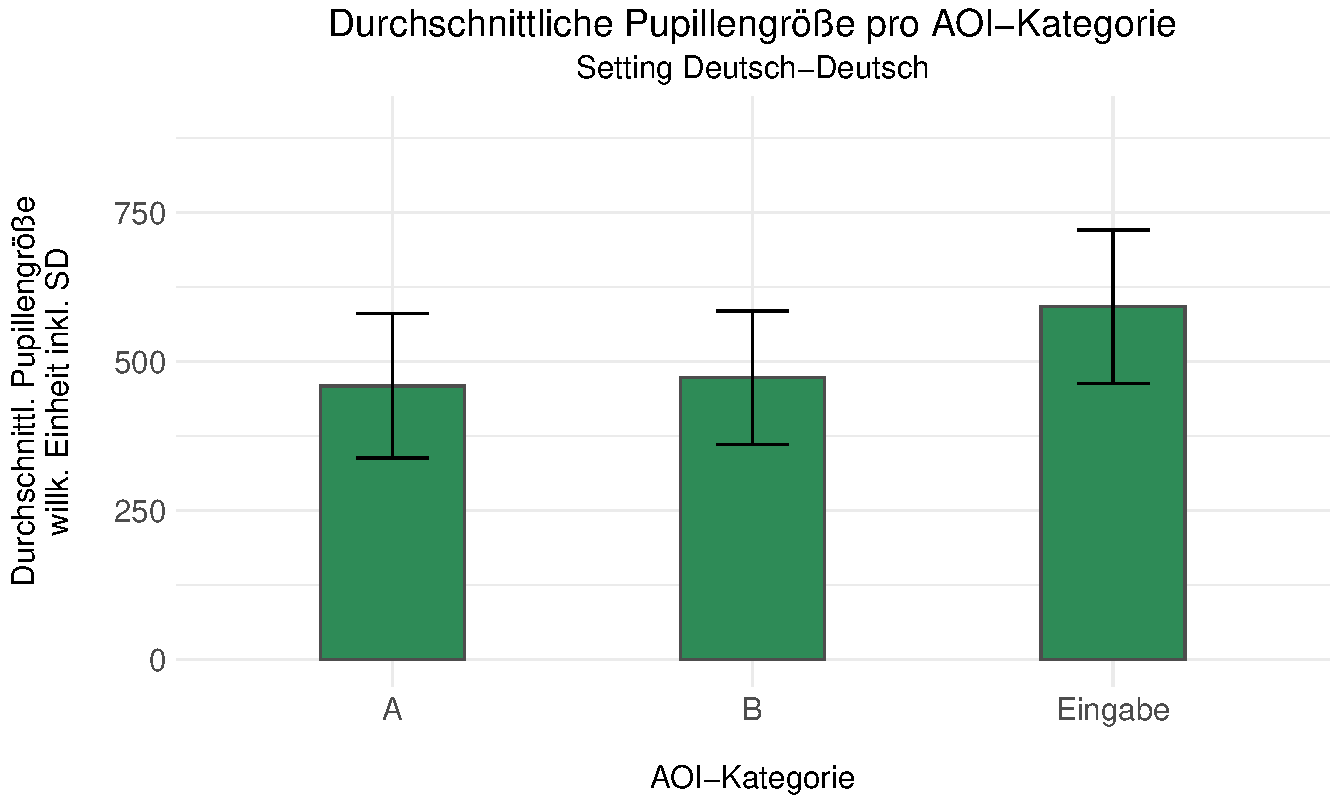
\includegraphics[width=.85\textwidth]{Figures/EyeTracking/DD/ggplot_DD_meanPSize_de}
	\caption{Durchschnittliche Pupillengröße pro AOI-Kategorie im Setting Deutsch-Deutsch}
	\label{K6:fig:DD:mean-error-psize}
\end{figure}

%------------------------------------------------------------------------

%------------------------------------------------------------------------

\begin{figure}
    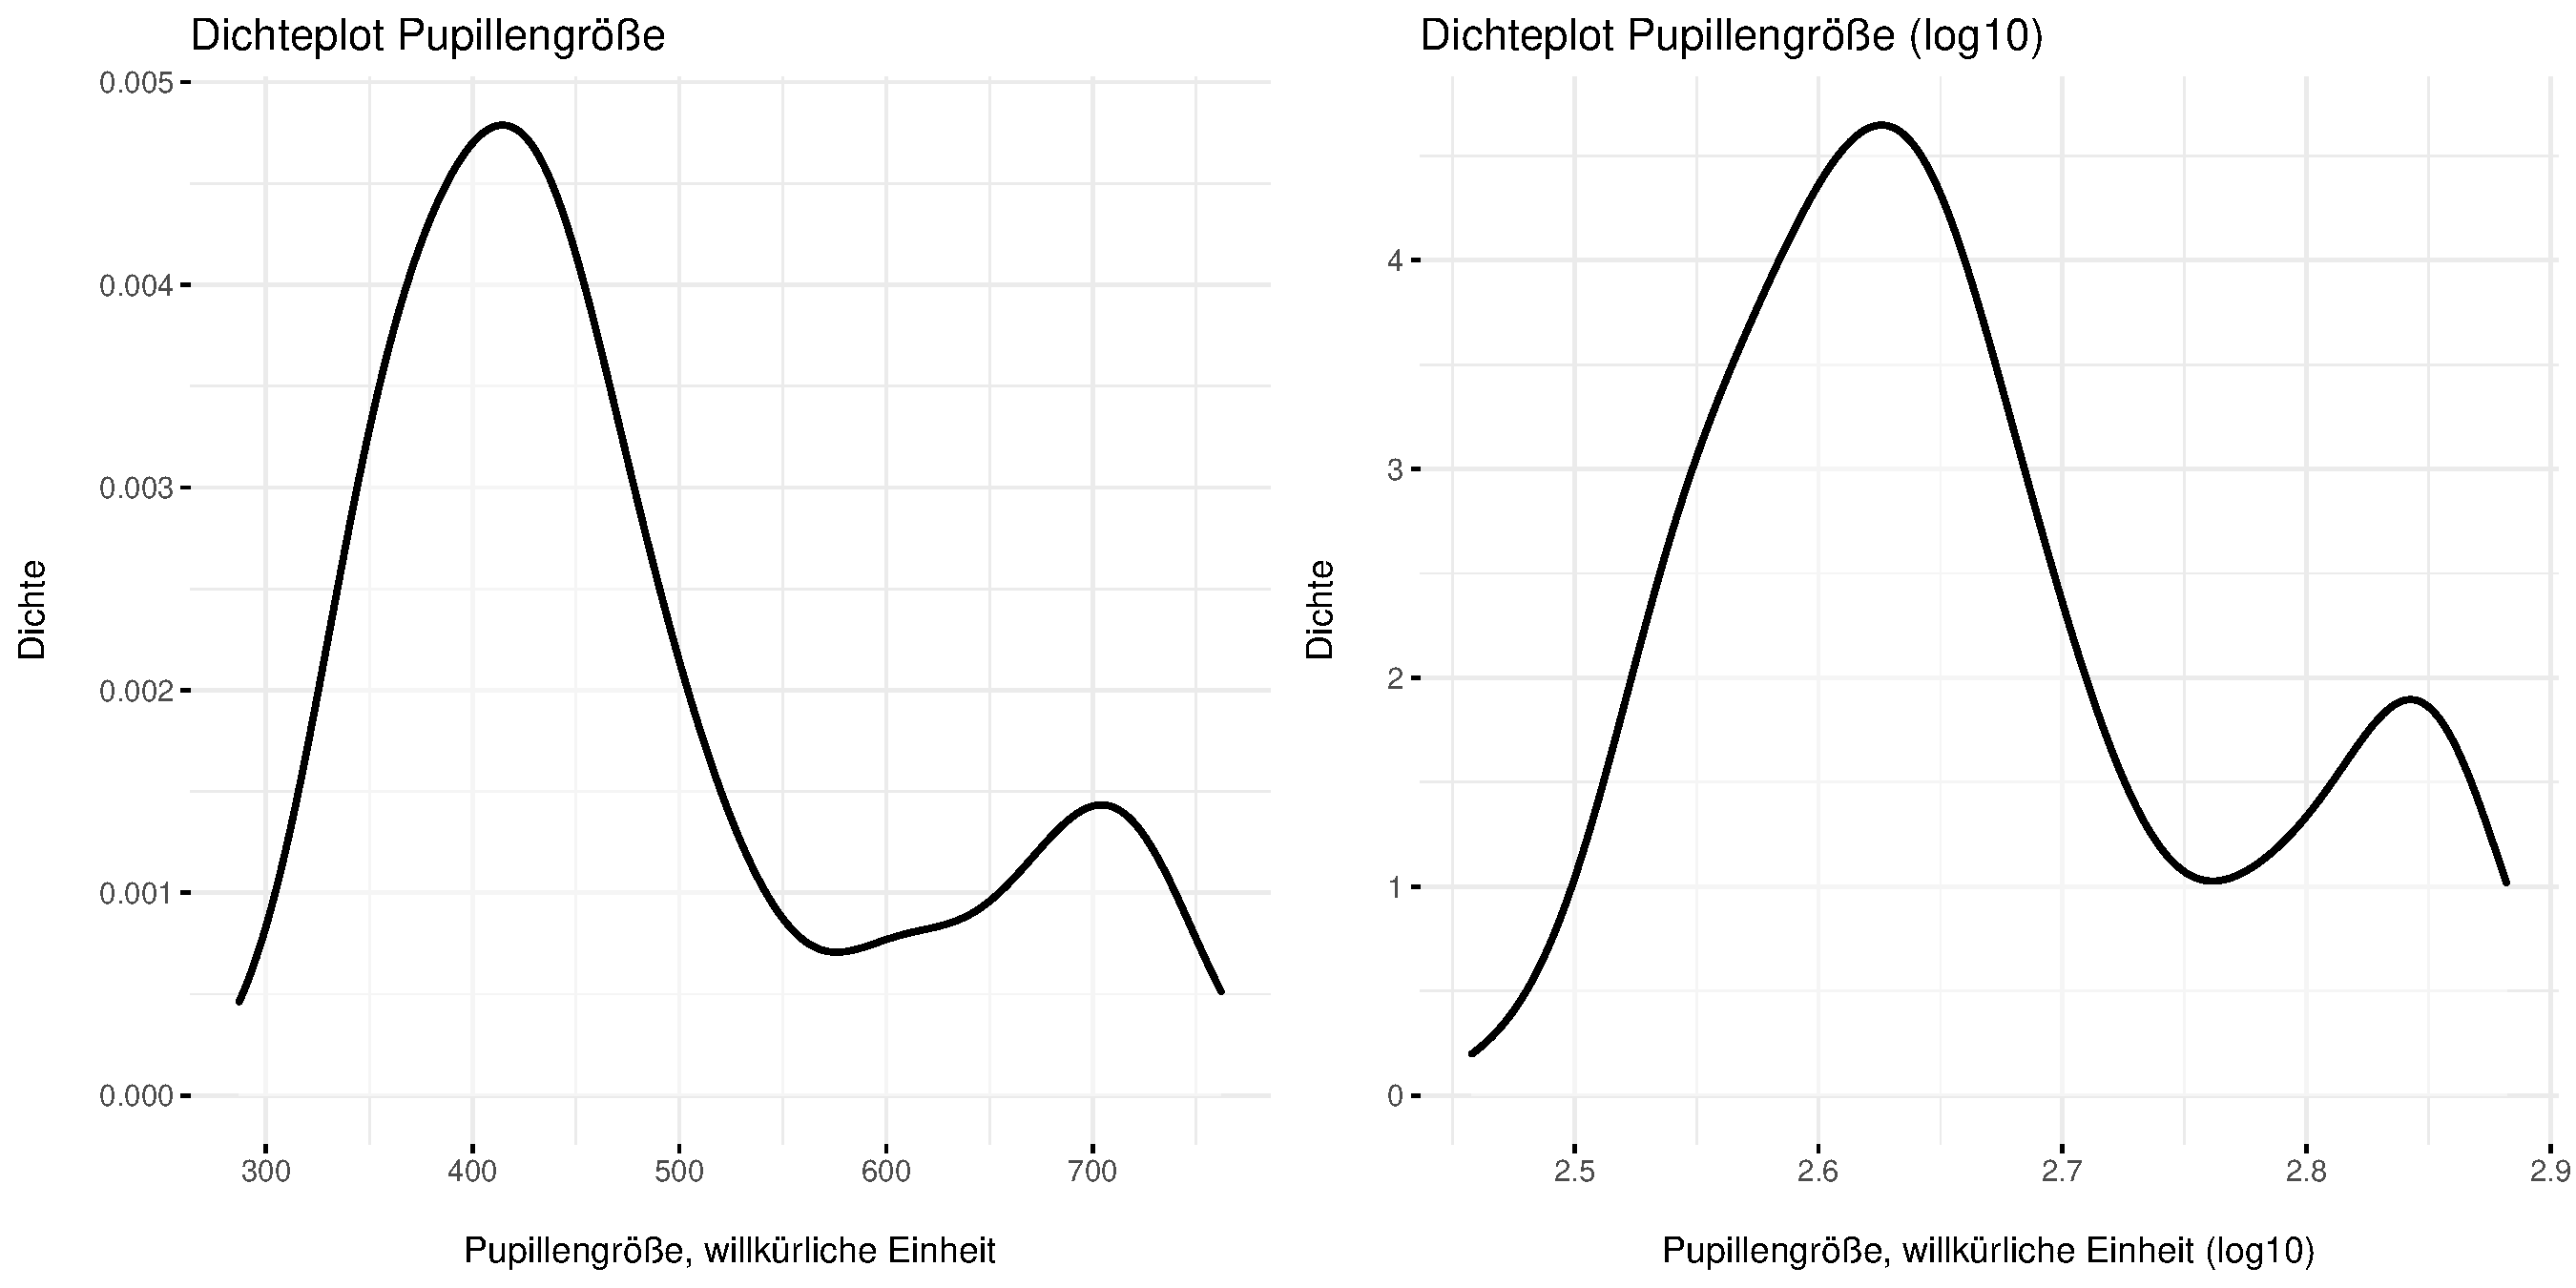
\includegraphics[width=\textwidth]{Figures/EyeTracking/DD/ggplot_DD-PSize_density_de}
	\caption{Verteilung der Pupillengröße in willkürlichen Einheiten: normal (links), logarithmisch transformiert (rechts)}
	\label{K6:fig:DD:density-PSize}
\end{figure}

%------------------------------------------------------------------------

Eine graphische Inspektion\is{Inspektion!graphische} der Daten (\figref{K6:fig:DD:density-PSize}) zeigt, dass weder die tatsächlichen noch die logarithmisch transformierten\is{Statistik!Transformation!logarithmische} Werte normalverteilt sind. Auch die statistische Untersuchung unter Anwendung des Shapiro-Wilk"=Tests\is{Shapiro-Wilk-Test}\is{Statistik!Testverfahren!Shapiro-Wilk-Test} deutet auf nicht normalverteilte Daten hin (roh: $W = 0,88, p < 0,001$, log10: $W = 0,93, p < 0,001$). Daher wird die Pupillengröße mit nicht-parametrischen Tests\is{Statistik!Testverfahren!nicht-parametrisches} untersucht.

Ein Kruskal-Wallis"=Test\is{Kruskal-Wallis-Test}\is{Statistik!Testverfahren!Kruskal-Wallis-Test} belegt, dass Unterschiede bei der Pupillengröße zwischen den einzelnen Teilnehmer{\textperiodcentered}innen bestehen ($\chi^2(6) = 152,19, p < 0,01$). Anschließend durchgeführte Post-hoc"=Tests (Dunn-Benjamini"=Hochberg-Tests)\is{Dunn-Benjamini-Hochberg-Test}\is{Statistik!Testverfahren!Dunn-Benjamini-Hochberg-Test} zeigen, dass die gruppierte Betrachtung von 15/21 (71,42\,\%) möglichen Paaren signifikante Unterschiede aufweist, sodass gefolgert werden kann, dass die Pupillengröße zwischen den Versuchspersonen variiert.

Ein zweiter Kruskal-Wallis"=Test\is{Kruskal-Wallis-Test}\is{Statistik!Testverfahren!Kruskal-Wallis-Test} deutet darauf hin, dass Unterschiede bei der Pupillengröße zwischen den einzelnen AOI-Kategorien bestehen ($\chi^2(6) = 8,68,\allowbreak\ p < 0,05$). Anschließend durchgeführte Post-hoc"=Tests (Dunn-Benjamini"=Hoch\-berg-Tests, s. \tabref{K6:tab:DeDe:dunntest-pupilsize})\is{Dunn-Benjamini-Hochberg-Test}\is{Statistik!Testverfahren!Dunn-Benjamini-Hochberg-Test} zeigen, dass sich die Kategoriegruppen \emph{A-Ein\-ga\-be} ($z = -2,74, p < 0,01, r = -0,2621229$) und \emph{B-Eingabe} ($z = -2,21, p < 0,05,\allowbreak\ r = -0,189165$) unterscheiden, sodass gefolgert werden kann, dass die Betrachtung der Eingabemaske einen signifikanten Einfluss auf die Pupillengröße hat, wobei die Effektgröße nur schwach ist.

%------------------------------------


\begin{table}
    \begin{tabular}{lS[table-format=-1.6]S[table-format=1.4{**}]S[table-format=1.2]}  
    \lsptoprule
        {AOI-Kategoriepaar} & {$z$} & {$p$ (angepasst)} & {Effekt}\\ 
        \midrule
        A-B       & -1,588856 & 0,0560 &  \\
        A-Eingabe & -2,736643 & 0,0093{**} & 0,26  \\ 
        B-Eingabe & -2,214119 & 0,0201{*} & 0,19 \\ 
        \lspbottomrule
    \end{tabular}
    \caption{Ergebnisse des Dunn-Tests: Gruppierte Vergleiche der Pupillengröße nach AOI-Kategorie\label{K6:tab:DeDe:dunntest-pupilsize}}
\end{table}


%------------------------------------

Es besteht hingegen ein signifikanter Unterschied in der zentralen Tendenz der Pupillengröße in Bezug auf die progressive erste Fixation\is{Fixation!progressive erste} zwischen den AOI, bei denen zuvor ein AOI mit höherer Ordnungszahl betrachtet wurde, und denen, die chronologisch betreten wurden (global: $U = 4.280,5, p < 0,001, r = 0,45$). Sowohl bei eigenen Chatbeiträgen als auch bei fremden zeigen sich signifikante Unterschiede bei der Pupillengröße, wenn zuvor ein AOI mit höherer Ordnungszahl betrachtet wurde als wenn es sich um eine tatsächliche chronologische erstmalige Fixation handelt. Der exakte Mann-Whitney"=U-Test\is{Mann-Whitney-U-Test}\is{Statistik!Testverfahren!Mann-Whitney-U-Test} für die eigenen Chatbeiträge ($U = 967,5, p < 0,01, r = 0,42$) in Verbindung mit einer Untersuchung der Effektstärke nach \citet{cohen_power_1992}\is{Cohen!Effektstärke nach}\is{Statistik!Testverfahren!Effektstärke nach Cohen} zeigt dabei einen mittleren Effekt. Bei fremden Chatbeiträgen weist der exakte Mann-Whitney"=U-Test\is{Mann-Whitney-U-Test}\is{Statistik!Testverfahren!Mann-Whitney-U-Test} ($U = 1.154,00, p < 0,001, r = 0,473$) ebenfalls einen mittleren Effekt auf (s. hierzu \tabref{K6:tab:DeDe:mwutest-pupilsize-ffixpro}).

%------------------------------------

\begin{table}
    \begin{tabular}{lrS[table-format=1.3{**}]r}  
    \lsptoprule
        {AOI-Kategorie} & \multicolumn{1}{c}{$U$} & {$p$ (angepasst)} & \multicolumn{1}{c}{Effekt} \\ 
        \midrule
        A & 967,5 & 0,001{**} & 0,42 \\ 
        B  & 1.154,0 & 0,001{**} & 0,47 \\ 
        Eingabe & n/a & {n/a} & -\\ 
        \midrule
        Global & 4.280,5 & 0,001{**} & 0,45 \\ 
        \lspbottomrule
    \end{tabular}
\caption{Ergebnisse des Mann-Whitney-U-Tests zur Pupillengröße nach AOI-Kategorie und progressiver ersten Fixation\label{K6:tab:DeDe:mwutest-pupilsize-ffixpro}}
\end{table}


%------------------------------------

Die Pupillengröße korreliert signifikant mit der Größe der AOI\is{Area of Interest!Größe des} ($r_{s} = -0,18,\allowbreak\ p < 0,01, n = 2.675.871$)\is{Spearman's Rho}\is{Korrelationstest nach Spearman}\is{Statistik!Testverfahren!Korrelationstest nach Spearman}. Dabei handelt es sich nach \citet{cohen_power_1992}\is{Cohen!Effektstärke nach}\is{Statistik!Testverfahren!Effektstärke nach Cohen} um einen schwachen Effekt. Das Bestimmtheitsmaß beträgt 3,1\,\%.
\is{Pupillengröße|)}


%------------------------------------------------------------------------

\subsection{Das sakkadische Blickverhalten}
\label{K6:subsec:sacGaze-DeDe}

%------------------------------------------------------------------------

\is{Sakkade!Anzahl an|(}Im Setting Deutsch-Deutsch werden generell mehr als drei Mal so viele Sakkaden im Bereich der Beiträge des Gegenübers getätigt wie jeweils auf den eigenen bzw. auf der Eingabemaske (s.\ \tabref{K6:tab:DeDe:sacspecs}), auf die zugleich die absolut wenigsten Sakkaden verfallen. Durchschnittlich werden hingegen in den eigenen und in den Beiträgen des Gegenübers etwa gleich viele Sakkaden gezählt. Die Mittelwerte betragen für ausgehende, eigene Nachrichten 9,76 Sakkaden und für eingehende, fremde Nachrichten 10,27 Sakkaden. Pro AOI im gesamten Datensatz werden im Schnitt 40,34 Sakkaden erfasst. Eine Berechnung der Werte für die Eingabemaske war nicht möglich, da es sich um ein statisches AOI handelt.

\begin{table}
    \begin{tabular}{lrrr}  
     \lsptoprule
        {AOI-Kategorie} & \multicolumn{1}{c}{Anzahl} & \multicolumn{1}{c}{Mittelwert} & \multicolumn{1}{c}{SD} \\ 
        \midrule
        A  & 781 & 9,76 & 4,36 \\ 
        B  & 2.557 & 10,27 & 5,08\\ 
        Eingabe   & 615 & n/a & n/a\\ 
        \midrule
        Global & 3.953 & 40,34 & 75.381,78\\ 
        \lspbottomrule
    \end{tabular}
    \caption{Anzahl, Mittelwert und SD der Sakkaden pro AOI-Ka\-te\-go\-rie\label{K6:tab:DeDe:sacspecs}}
\end{table}

%------------------------------------


\tabref{K6:tab:saccount:direction:DeDe} stellt die aufsummierte Sakkadenanzahl nach Richtung und AOI-Kategorie dar. Sakkaden, die außerhalb eines AOI gelandet sind, werden unter \emph{NA} gezählt. In absoluten Zahlen fällt auf, dass innerhalb der AOI-Kategorie \emph{B} mehr Sakkaden erfolgen als in den anderen beiden Kategorien. Rechtsgerichtete Sakkaden dominieren in jeder Kategorie. Das ist nicht weiter verwunderlich, da das Deutsche der Leserichtung von links nach rechts folgt. Auffällig sind hingegen die vergleichsweise vielen Sakkaden nach links und nach oben in der Kategorie \emph{B}.

%------------------------------------------------------------------------

%%%% Multi-Table: 2x2, wobei nur 2x1 Kacheln belegt sind mit den jeweiligen Kategorien A,B, Eingabe

\begin{table}
    \begin{minipage}{0.5\textwidth}\centering
        \begin{tabular}{lrr} \lsptoprule
         Kategorie & \multicolumn{2}{c}{{A}} \\ 
         \cmidrule(lr){2-3}
            \multicolumn{1}{c}{Richtung} & \multicolumn{1}{c}{Anzahl} & \multicolumn{1}{c}{Prozent} \\ 
            \midrule
            Runter & 33 & 4,23 \\ 
            Links & 168 & 21,51 \\ 
            Rechts & 531 & 67,99 \\ 
            Hoch & 13 & 4,61 \\ 
            \emph{NA} & 13 & 1,66 \\
            \midrule
            {Gesamt} & 781 & 100 \\ 
            \lspbottomrule
            \end{tabular}
            \end{minipage}\begin{minipage}{0.5\textwidth}\centering
            \begin{tabular}{lrr} 
            \lsptoprule
            Kategorie & \multicolumn{2}{c}{{B}} \\ 
            \cmidrule(lr){2-3}
            \multicolumn{1}{c}{Richtung} & \multicolumn{1}{c}{Anzahl} & \multicolumn{1}{c}{Prozent}  \\ 
            \midrule
            Runter & 62 & 2,42 \\ 
            Links & 611 & 24,90 \\ 
            Rechts & 1.661 & 64,96 \\ 
            Hoch & 177 & 6,92 \\ 
            \emph{NA} & 46 & 1,80 \\ 
            \midrule
            {Gesamt} & 2.557 & 100 \\ 
            \lspbottomrule
         \end{tabular}    
    \end{minipage}\medskip\\
    \begin{minipage}{0.5\textwidth}\centering
            \begin{tabular}{lrr} 
            \lsptoprule
            Kategorie & \multicolumn{2}{c}{{Eingabe}} \\ 
            \cmidrule(lr){2-3}
            \multicolumn{1}{c}{Richtung} & \multicolumn{1}{c}{Anzahl} & \multicolumn{1}{c}{Prozent}  \\ 
            \midrule
            Runter & 102 & 16,59 \\ 
            Links & 205 & 33,33 \\ 
            Rechts & 268 & 43,58 \\ 
            Hoch & 25 & 4,07 \\ 
            \emph{NA} & 15 & 2,44 \\ 
            \midrule
            {Gesamt} & 615 & 100 \\ 
            \lspbottomrule
         \end{tabular}    
    \end{minipage}
      \caption{Sakkadenanzahl nach Richtung und AOI-Kategorie im Setting Deutsch-Deutsch}
    \label{K6:tab:saccount:direction:DeDe}
\end{table}

%------------------------------------------------------------------------
\is{Sakkade!Anzahl an|)}

%------------------------------------------------------------------------

\subsubsection{Sakkadenamplitude}
\label{K6:subsubsec:sacamp:DeDe}

%------------------------------------------------------------------------

\is{Sakkade!-namplitude|(}
Die durchschnittliche Sakkadenamplitude (s. \tabref{K6:tab:DeDe:sacamp}) bei Betrachtung der eingehenden Nachrichten liegt mit 1,95°/ms unterhalb des Gesamtschnittes, die der Eingabemaske (1,85\,°/ms) und der ausgehenden Nachrichten (1,81\,°/ms) oberhalb des Gesamtschnittes (1,84\,°/ms). 

%------------------------------------

\begin{table}
    \begin{tabular}{lccr}  
    \lsptoprule
        {AOI-Kategorie} & {Mittelwert} & {Median} & \multicolumn{1}{c}{SD} \\ 
        \midrule
        A  & 1,95 & 1,42 & 1,6 \\
        B  & 1,81 & 1,38 & 1,39\\ 
        Eingabe   & 1,85 & 1,20 & 1,70\\ 
        \midrule
        Global  & 1,84 & 1,36 & 1,49\\ 
        \lspbottomrule
    \end{tabular}
    \caption[Mittelwert, Median und SD der Sakkadenamplitude]{Mittelwert, Median und SD der Sakkadenamplitude pro AOI-Kategorie}
    \label{K6:tab:DeDe:sacamp}
\end{table}

%------------------------------------

Der Anderson-Darling"=Test\is{Statistik!Testverfahren!Anderson-Darling-Test}\is{Anderson-Darling-Test} zeigt, dass sowohl die Gesamtheit des Datensatzes als auch der Datensatz nach einzelnen AOI-Kategorien in Bezug auf die Sakkadenamplitude nicht normalverteilt ist. Der AD-Test weist ein Ergebnis von ($A = 429,07, p < 0,01$) für den gesamten Datensatz auf und für die Kategorien \emph{A}: ($A = 85,64, p < 0,01$), \emph{B}: ($A = 262,37, p < 0,01$) und Eingabe: ($A = 80,89,\allowbreak\ p < 0,01$). Auch eine logarithmische Transformation\is{Statistik!Transformation!logarithmische} änderte die Verteilung nicht wesentlich (s. \figref{K6:fig:DeDe:sacamp-density}). Auf die Kategorie \emph{A} verfallen 781 Sakkaden, 2.557 auf \emph{B} und 615 auf die Eingabemaske. Insgesamt enthält der Datensatz somit 3.953 Sakkaden.

%------------------------------------------------------------------------

\begin{figure}
	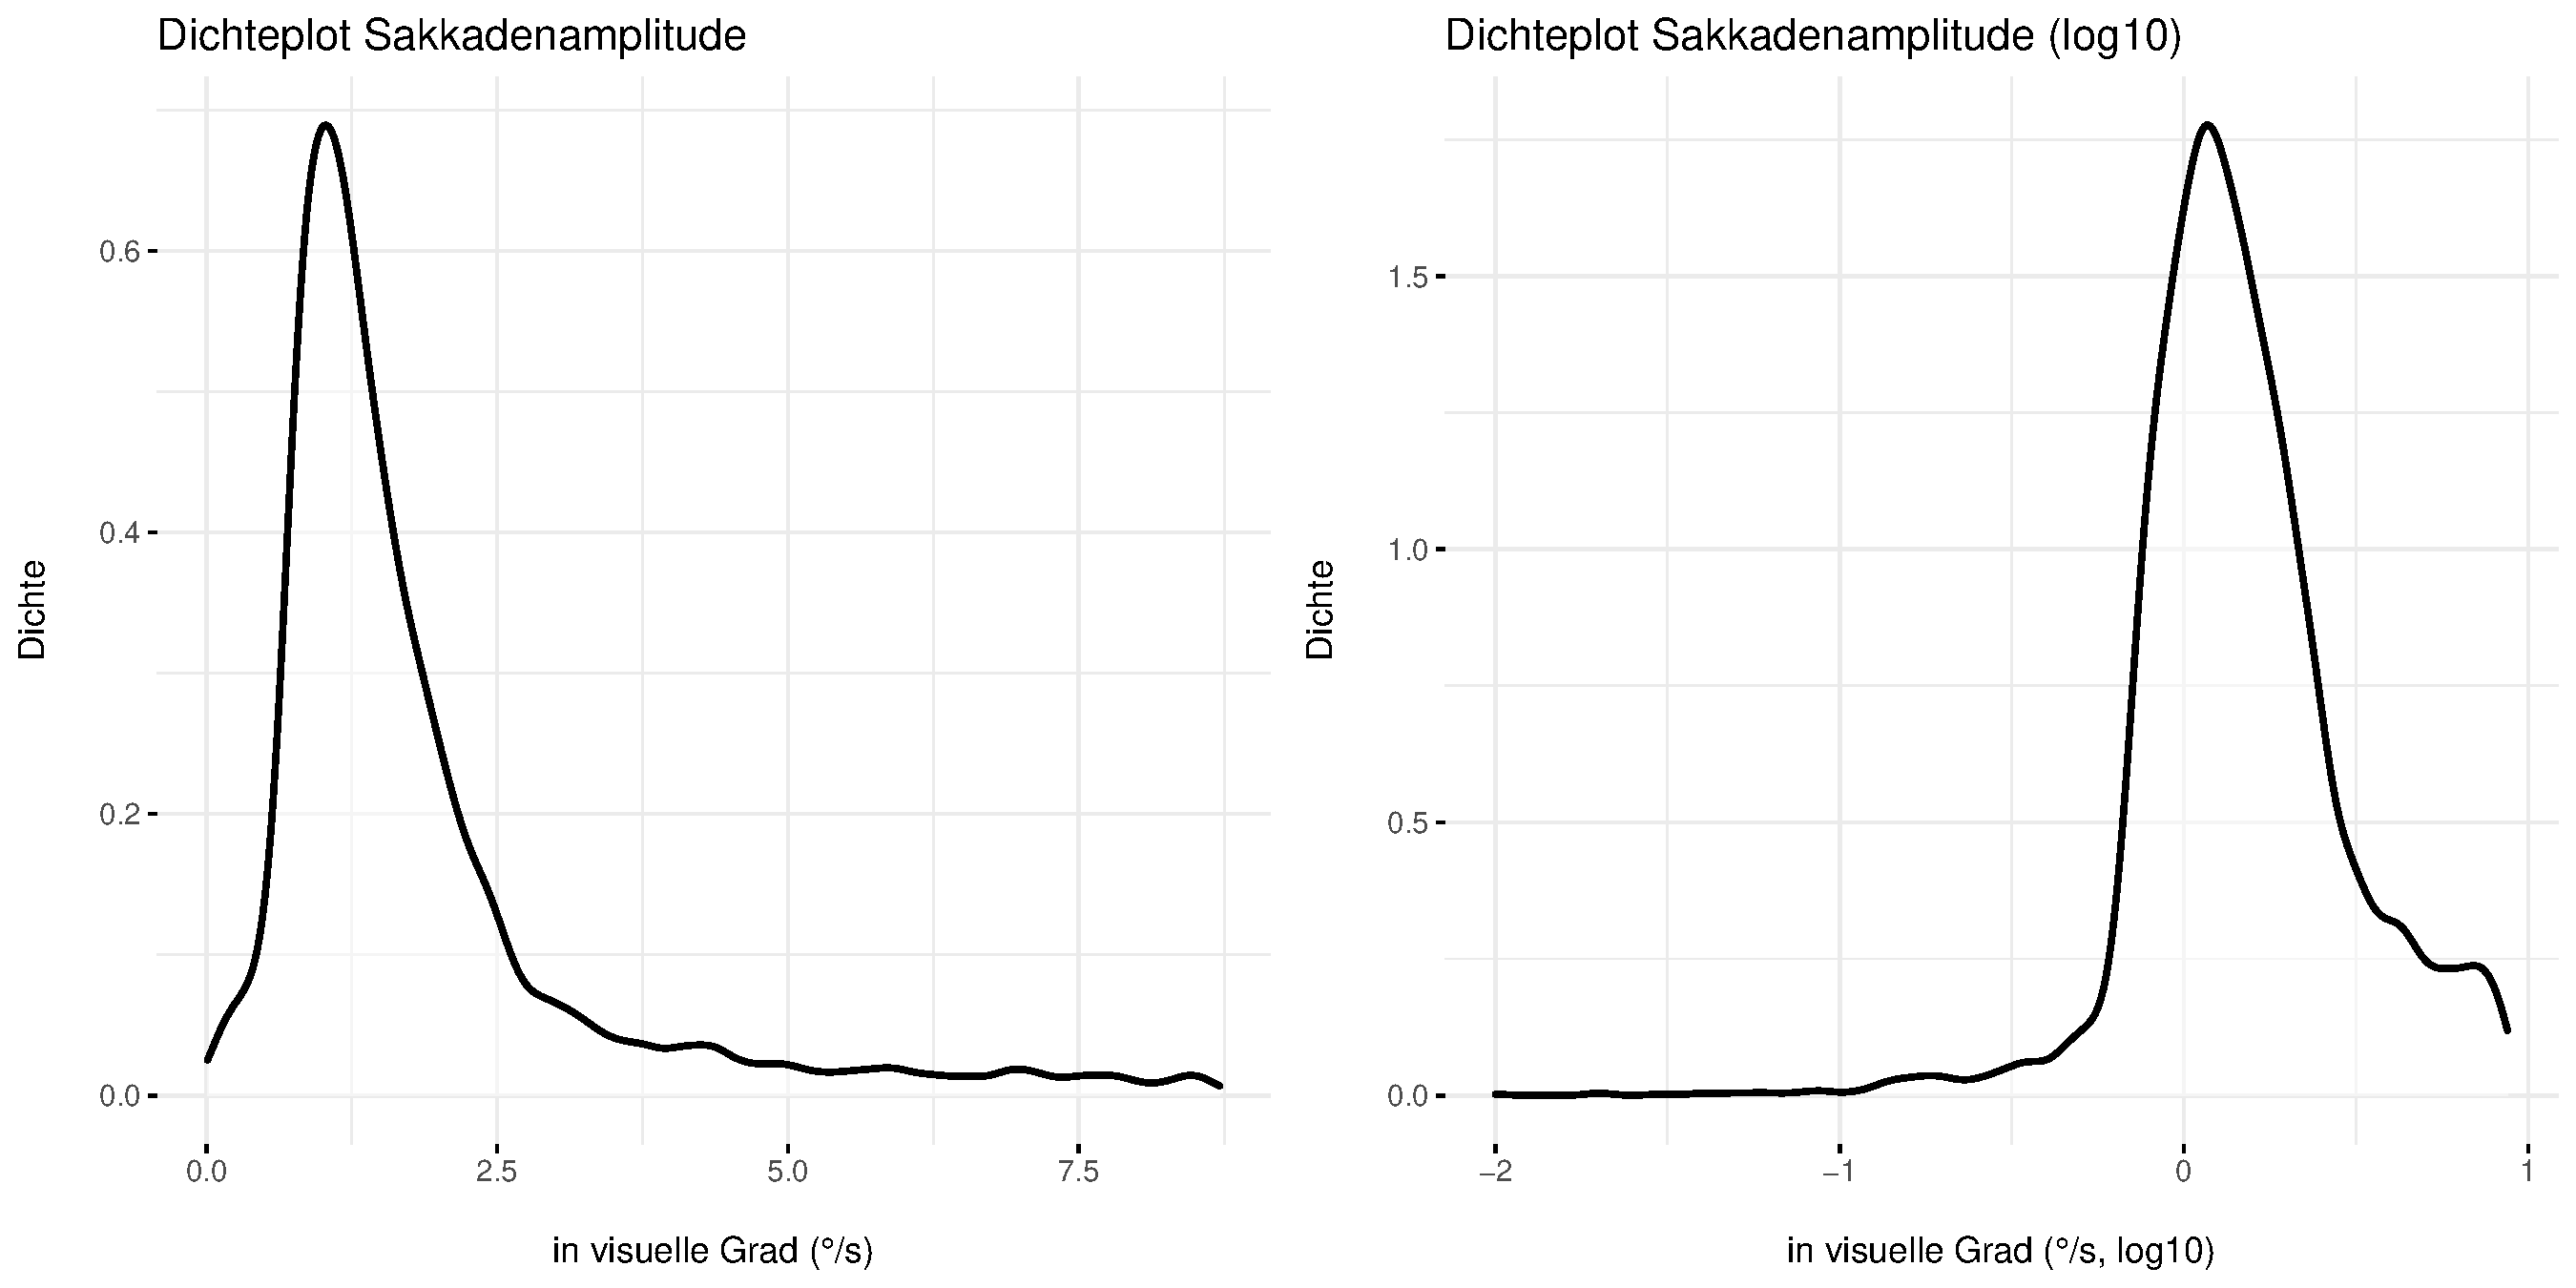
\includegraphics[width=\textwidth]{Figures/EyeTracking/DD/ggplot_DD-SacAmp_density_de}
	\caption{Verteilung der Sakkadenamplitude: normal (links), logarithmisch transformiert (rechts)}
	\label{K6:fig:DeDe:sacamp-density}
\end{figure}

%------------------------------------------------------------------------

Wie auch im Falle der Sakkadenamplitude und -dauer im Setting Katalanisch-Deutsch (s. S.\,\pageref{K6:subsec:sacGaze-CatDe}) wurde die Korrelation beider Variablen untersucht. Für das Setting Deutsch-Deutsch ergeben sich folgende Werte aus dem Korrelationstest nach Spearman's Rho\is{Spearman's Rho}\is{Korrelationstest nach Spearman}\is{Statistik!Testverfahren!Korrelationstest nach Spearman}: Sowohl der gesamte Datensatz als auch die Werte nach einzelnen AOI-Kategorien getrennt stehen in einer signifikant positiven Beziehung zueinander -- Gesamt: ($S = 8.037.112.694, p < 0,01, r = 0,63$), \emph{A}: ($S = 48.444.315, p < 0,01, r = 0,66$) und \emph{B}: ($S = 1.979.782.735, p < 0,01, r = 0,66$). Für die Eingabemaske lagen zu wenig Datenpunkte vor, als dass eine Berechnung möglich gewesen wäre.

Ein Kruskal-Wallis"=Test\is{Kruskal-Wallis-Test}\is{Statistik!Testverfahren!Kruskal-Wallis-Test} belegt, dass Unterschiede bei der Sakkadenamplitude zwischen den einzelnen Teilnehmer{\textperiodcentered}innen bestehen ($\chi^2(6) = 81,54, p < 0,01$). Anschließend durchgeführte Post-hoc"=Tests (Dunn-Benjamini"=Hochberg-Tests)\is{Dunn-Benjamini-Hochberg-Test}\is{Statistik!Testverfahren!Dunn-Benjamini-Hochberg-Test} zeigen, dass sich 14 von 21 möglichen Paaren (66,67\,\%) signifikant voneinander unterscheiden, sodass gefolgert werden kann, dass die Sakkadenamplitude in gewissem Maße von der Individualität der TN abhängt.\largerpage

Ein weiterer Kruskal-Wallis"=Test\is{Kruskal-Wallis-Test}\is{Statistik!Testverfahren!Kruskal-Wallis-Test} zeigt, dass Unterschiede bei der Sakkadenamplitude zwischen den einzelnen AOI"=Kategorien bestehen ($\chi^2(2) = 30,63,\allowbreak\ p < 0,01$). Anschließend durchgeführte Post-hoc"=Tests (Dunn-Benjamini"=Hochberg-Tests)\is{Dunn-Benjamini-Hochberg-Test}\is{Statistik!Testverfahren!Dunn-Benjamini-Hochberg-Test} zeigen, dass sich die AOI"=Kategorien \emph{A-Eingabe} und \emph{B-Eingabe} signifikant unterscheiden. Im Falle des Paares \emph{A-Eingabe} gilt ($z = 17, p < 0,01, r = 0,12$) und der Kategorie \emph{B-Eingabe} ($z = 4,83, p < 0,01, r = 0,08$), sodass gefolgert werden kann, dass die Sakkadenamplitude von der AOI"=Kategorie abhängt (s. \tabref{tab:DeDe:dunntest-sacamp}), der Asterisk zeigt das Signifikanzlevel an: *$ \alpha{} < 0,05$).

%------------------------------------

\begin{table}
    \begin{tabular}{lS[table-format=1.6]S[table-format=1.4{***}]c}  
    \lsptoprule
        {AOI-Kategoriepaar} & {$z$} & {$p$ (angepasst)} & {Effekt}\\\midrule
        A-B & 1,591889 & 0,0557 & -\\
        A-Eingabe & 5,174487 & 0,0000{***} & 0,12 \\ 
        B-Eingabe  &  4,829444 & 0,0000{***} & 0,08\\ 
        \lspbottomrule
    \end{tabular}
    \caption{Ergebnisse des Dunn-Tests: Gruppierte Vergleiche der Sakkadenamplitude nach AOI-Kategorie\label{tab:DeDe:dunntest-sacamp}}
\end{table}

%------------------------------------

Die Tests im Setting Deutsch-Deutsch belegen signifikante Unterschiede in der Sakkadenamplitude für die Vergleichspaare mit Beteiligung der Eingabemaske. Die vergleichende Untersuchung der eigenen vs. fremden Beiträge bleibt unauffällig.

%------------------------------------------------------------------------

\begin{figure}
	\includegraphics[width=.85\textwidth]{Figures/EyeTracking/DD/ggplot_DD-boxplot_sacamp_AOI_de}
	\caption{Sakkadenamplitude pro AOI}
	\label{K6:fig:DeDe:sacamp-box}
\end{figure}

%------------------------------------------------------------------------
\is{Sakkade!-namplitude|)}

%------------------------------------------------------------------------

\subsubsection{Sakkadendauer}
\label{K6:subsubsec:sacdur:DD}\largerpage[2]

%------------------------------------------------------------------------

\is{Sakkade!-ndauer|(}
\tabref{K6:tab:DeDe:sacdur-mean-sd} stellt Mittelwert und Standardabweichung der Sakkadendauer pro AOI-Kategorie dar. Die Sakkaden im Bereich der ausgehenden Nachrichten dauern im Schnitt 1,8\,ms länger als im Bereich der Nachrichten des Gegenübers. Auf den gesamten Datensatz bezogen beträgt die durchschnittliche Sakkadendauer 31,83\,ms und liegt damit zwischen den Mittelwerten der beiden Beitragsarten.

Der Anderson-Darling"=Test\is{Statistik!Testverfahren!Anderson-Darling-Test}\is{Anderson-Darling-Test} zeigt, dass sowohl die Gesamtheit des Datensatzes als auch der Datensatz nach einzelnen AOI-Kategorien in Bezug auf die Sakkadendauer nicht normalverteilt ist. Es ergibt sich für die Gesamtheit ein Verteilungswert im AD-Test von ($A = 935, p < 0,01$) und für die Kategorien \emph{A}: ($A = 165,76, p < 0,01$), \emph{B}: ($A = 634,64,\allowbreak\ p < 0,01$) und Eingabe: ($A = 138,21, p < 0,01$). Auch eine logarithmische Transformation\is{Statistik!Transformation!logarithmische} änderte die Verteilung nicht wesentlich (s. \figref{K6:fig:DeDe:sacdur-density}). Auf die Kategorie \emph{A} verfallen somit noch 952 Sakkaden, 3.279 auf \emph{B} und 847 auf die Eingabemaske. Insgesamt enthält der Datensatz 5.078 Sakkaden. Die durchschnittliche Sakkadendauer bei der Betrachtung eingehender Nachrichten liegt unterhalb des Gesamtschnittes, die der ausgehenden Nachrichten und der Eingabemaske überhalb des Schnittes.\largerpage[-1]

%------------------------------------

\begin{table}
    \begin{tabular}{lccc}  
    \lsptoprule
        {AOI-Kategorie} & {Mittelwert} & {Median} & {SD} \\ 
        \midrule
        A  & 32,90 & 21 & 33,00 \\
        B  & 31,10 & 20 & 32,01 \\ 
        Eingabe & 33,44 & 22 & 33,69 \\ 
        \midrule
        Global  &31,83 & 21 & 32,49 \\ 
        \lspbottomrule
    \end{tabular}
    \caption[Mittelwert, Median und SD der Sakkadendauer]{Mittelwert, Median und SD der Sakkadendauer pro AOI-Kategorie}
    \label{K6:tab:DeDe:sacdur-mean-sd}
\end{table}

%------------------------------------

%------------------------------------------------------------------------

\begin{figure}
    \includegraphics[width=\textwidth]{Figures/EyeTracking/DD/ggplot_DD-SacAmp_density_de}
	\caption{Verteilung der Sakkadendauer: normal (links), logarithmisch transformiert (rechts)}
	\label{K6:fig:DeDe:sacdur-density}
\end{figure}

%------------------------------------------------------------------------

Ein Kruskal-Wallis"=Test\is{Kruskal-Wallis-Test}\is{Statistik!Testverfahren!Kruskal-Wallis-Test} deutet darauf hin, dass Unterschiede bei der Sakkadendauer zwischen den einzelnen Teilnehmer{\textperiodcentered}innen bestehen ($\chi^2(6) = 53,66,\allowbreak\ p < 0,01$). Anschließend durchgeführte Post-hoc"=Tests (Dunn-Benjamini"=Hochberg-Tests)\is{Dunn-Benjamini-Hochberg-Test}\is{Statistik!Testverfahren!Dunn-Benjamini-Hochberg-Test} zeigen, dass sich 12 von 21 (57,14\,\%) TN-Gruppen signifikant unterscheiden, sodass gefolgert werden kann, dass die Sakkadendauer in gewissem Maße von der Individualität der TN abhängt.\largerpage

%------------------------------------

\begin{table}
    \begin{tabular}{lS[table-format=-1.6]S[table-format=1.4{**}]c}
    \lsptoprule
        {AOI-Kategoriepaar} & {$z$} & {$p$ (angepasst)} & {Effekt}\\\midrule
        A-B & 2,800713 & 0,0076{**} & 0,04 \\ 
        A-Eingabe & 0,318257 & 0,3751 & - \\ 
        B-Eingabe  &  -2,285139 & 0,0167{*} & 0,04 \\
        \lspbottomrule
        \end{tabular}
        \caption{Ergebnisse des Dunn-Tests: Gruppierte Vergleiche der Sakkadendauer nach AOI-Kategorie}
    \label{tab:DeDe:dunntest-sacdur}
\end{table}

%------------------------------------

Ein weiterer Kruskal-Wallis"=Test\is{Kruskal-Wallis-Test}\is{Statistik!Testverfahren!Kruskal-Wallis-Test} belegt, dass Unterschiede bei der Sakkadendauer zwischen den einzelnen AOI"=Kategorien bestehen ($\chi^2(2) = 10,81,\allowbreak\ p < 0,01$). Anschließend durchgeführte Post-hoc"=Tests (Dunn-Benjamini"=Hochberg-Tests\is{Dunn-Benjamini-Hochberg-Test}\is{Statistik!Testverfahren!Dunn-Benjamini-Hochberg-Test}, s. \tabref{tab:DeDe:dunntest-sacdur}, der Asterisk zeigt das Signifikanzlevel an: * $\alpha{} < 0,05$) zeigen, dass sich die AOI-Kategorien \emph{A-B} und \emph{B-Eingabe} signifikant unterscheiden. Somit kann gefolgert werden, dass die Sakkadendauer von der AOI-Kategorie abhängt.

%------------------------------------------------------------------------

\begin{figure}
	\includegraphics[width=.85\textwidth]{Figures/EyeTracking/DD/ggplot_DD-boxplot_sacdur_AOI_de}
	\caption{Sakkadendauer pro AOI}
	\label{K6:fig:DeDe:sacdur-mean}
\end{figure}

%------------------------------------------------------------------------

\is{Sakkade!-ndauer|)}

%------------------------------------------------------------------------

\subsection{Zusammenfassung der Ergebnisse der einsprachigen Vergleichsstudie}
\label{K6:subsec:resumee:DeDe}\largerpage

%------------------------------------------------------------------------

Für die Vergleichsstudie wurden weniger Versuchspersonen rekrutiert als für die Untersuchung des Skype Translators. Damit einher geht auch ein verkürzter Versuchsaufbau, der nicht mit einem Abschlussfragebogen\is{Fragebogen!Ausgangs-} endet, in dem die Proband{\textperiodcentered}innen ihre Eindrücke zu der maschinell übersetzten Kommunikationssituation\is{Kommunikation!-ssituation} darlegen sollen. Ziel dieser Vergleichsstudie ist es vielmehr, okulometrische Referenzdaten zu generieren, die die Wahrnehmung der Versuchsteilnehmer{\textperiodcentered}innen im Setting Katalanisch-Deutsch kontrastieren.

Die Auswertung des Eingangsfragebogens\is{Fragebogen!Eingangs-} zu Beginn der Studie zeugt von einer variabel zusammengesetzten Kohorte. Alle sieben Personen sind Studierende der Universität Leipzig. Es handelt sich um junge Menschen Anfang 20, die einerseits mehrere Fremdsprachen sprechen und andererseits auch mehrheitlich bereits Auslandserfahrung aufweisen können. Wie auch im anderen Versuch ist Skype\is{Skype} für die Versuchspersonen nicht die präferierte Software für den Kontakt mit Freunden, Familie und anderen Menschen. Zugleich ist der Funktionsumfang von Skype nicht gänzlich unbekannt.

Mit Blick auf alle untersuchten Indikatoren wird ein Leseverhalten charakterisiert, das besonders die Eingabemaske und die eingehenden Textnachrichten des Gegenübers in den Fokus rückt. Dies wird bereits durch die Betrachtung der Bildschirmaufnahmen visuell\is{Inspektion!visuelle} ersichtlich. Es wirkt allerdings so, als wiesen die Indikatoren in diesem einsprachigen Setting eine breitere Streuung über den Bildschirm auf als im anderen Versuchsaufbau. Diese Beobachtung ist vorläufig und daher mit Vorsicht auszusprechen. Eine eingehende Untersuchung sollte vorgenommen werden. Die fremden Beiträge werden sowohl absolut-numerisch als auch statistisch mehr betrachtet. Wie auch im katalanisch-deutschen Versuchsaufbau sind die Erkenntnisse, die aus den Daten der Eingabemaske gezogen werden können, nur begrenzt interpretierbar. Die Eingabemaske wurde auch hier als statisches AOI\is{Area of Interest!statisches} annotiert, somit sind Indikatoren, die auf ein erstmaliges Ereignis abzielen, auch tatsächlich immer nur als das erstmalige, singuläre Ereignis zu verstehen, selbst wenn die Eingabemaske im weiteren Verlauf der Studie erneut oder insgesamt mehrmals betrachtet wurde. Die in der Zusammenfassung zur katalanisch-deutschen Studie erwähnten interpretierbaren Indikatoren (Fixationszahl und Gesamtverweildauer, s. Abschnitt \,\ref{K6:subsec:resumee:CatDe}, S.\,\pageref{K6:subsec:resumee:CatDe}) gelten auch hier.

Im Gegensatz zur Analyse der Regressionen im anderen Studienteil war es in diesem Fall nur begrenzt möglich, entsprechende Regressionsmodelle zur Untersuchung zu erstellen. Es lassen sich dennoch wenige, begrenzte Annahmen aufstellen. Einerseits liegt die Vermutung nahe, dass die Versuchspersonen im deutsch-deutschen Setting noch einmal zu den eingehenden Nachrichten des Gegenübers zurückspringen, um die erhaltenen Informationen mit den eigenen Beiträgen abzugleichen. Dies kann sowohl für die bereits gesendeten Nachrichten (\emph{A}) gelten als auch für Nachrichten, die die Proband{\textperiodcentered}innen gerade im Begriff sind zu verfassen und sich daher noch im AOI der Eingabemaske befinden.

Im Gegensatz zur Sakkadenamplitude weisen die Tests der Sakkadendauer auf signifikante Unterschiede zwischen den eigenen und fremden Beiträgen sowie den fremden Beiträgen und der Eingabemaske hin. Hieraus lässt sich die Annahme ableiten, dass die Beiträge des Gegenübers anders wahrgenommen und verarbeitet werden als einerseits der Text während der Produktion in der Eingabemaske als auch das Rezipieren der eigenen Beiträge.
